\def\eprintversion{0}
\def\vertempyd{0}

\ifnum\eprintversion=0
	\documentclass{llncs}
	\newtheorem{myclaim}[theorem]{Claim}
	% \newtheorem{myclaim}{Claim}[section]
	\newtheorem{fact}[theorem]{Fact}
    % \usepackage[paper=letterpaper,margin=1in]{geometry}    
\usepackage{booktabs}
\usepackage{microtype}
\else
\documentclass[11pt,letterpaper]{article}
\usepackage[paper=letterpaper,margin=1in]{geometry}    
\usepackage{amsthm}
\usepackage{booktabs}

\usepackage{microtype}

	\theoremstyle{plain}
	\newtheorem{theorem}{Theorem}[section]
	\newtheorem{lemma}[theorem]{Lemma}
	\newtheorem{corollary}[theorem]{Corollary}
	\newtheorem{observation}[theorem]{Observation}
	\newtheorem{fact}[theorem]{Fact}
	\newtheorem{remark}[theorem]{Remark}
	\newtheorem{myclaim}[theorem]{Claim}
	\newtheorem{notation}[theorem]{Notation}
	\theoremstyle{definition}
	\newtheorem{definition}[theorem]{Definition}
	\newtheorem{proposition}[theorem]{Proposition}
	\fi

\usepackage[table]{xcolor}
\usepackage{wrapfig}

\usepackage{tabularx}
\usepackage{multirow}
\usepackage{graphicx} 
\usepackage{enumerate}
\usepackage{enumitem}
\usepackage{tikz}
\usepackage{amsmath}
\usepackage{aliascnt,lscape}
\usepackage{amsfonts}
%\usepackage{authblk}
\usepackage{mdframed}
\usepackage{caption}
\usepackage{subcaption}


\usepackage{amssymb}
%\usepackage{color} 
\usepackage{multicol}
\usepackage{calc}
\usepackage{subcaption}
\ifnum\eprintversion=1
\usepackage[%pagebackref,
			colorlinks=true,
			linkcolor=blue,
			citecolor=blue,
			pdftitle={sublinear-pir-improved},
    		pdfauthor={anonymous}]{hyperref}
\else
\usepackage[
			colorlinks=true,
			linkcolor=blue,
			citecolor=blue,
			pdftitle={sublinear-pir-improved},
    		pdfauthor={anonymous}]{hyperref}
\fi
\usepackage{colonequals}  % for \ratio in :<=>
\usepackage{cleveref}

\usepackage{wrapfig}
\usepackage{float}
\usepackage{thm-restate}
\usepackage{xstring}
\usepackage{pifont}
\usepackage{xspace}
\usepackage{orcidlink}

\usetikzlibrary{arrows.meta}
\tikzset{>={Latex[width=0.5mm,length=1mm]}}

\usetikzlibrary{decorations.pathreplacing}
% !TEX root = main.tex
%Section: Macros
\newcommand{\MyAtop}[2]{\genfrac{}{}{0pt}{}{#1}{#2}}
\newcommand{\qedsymb}{\hfill{\rule{2mm}{2mm}}}
\renewenvironment{proof}{\begin{trivlist} \item[\hspace{\labelsep}{\bf
\noindent Proof.\/}] }{\qedsymb\end{trivlist}}


%%%%%%%%%%%%%%%%%%%
% Generic Macros
%%%%%%%%%%%%%%%%%%%
\newcommand{\bA}{\mathbf{A}}
\newcommand{\bB}{\mathbf{B}}
\newcommand{\bC}{\mathbf{C}}
\newcommand{\bD}{\mathbf{D}}
\newcommand{\bE}{\mathbf{E}}
\newcommand{\bF}{\mathbf{F}}
\newcommand{\bG}{\mathbf{G}}
\newcommand{\bH}{\mathbf{H}}
\newcommand{\bI}{\mathbf{I}}
\newcommand{\bJ}{\mathbf{J}}
\newcommand{\bK}{\mathbf{K}}
\newcommand{\bL}{\mathbf{L}}
\newcommand{\bM}{\mathbf{M}}
\newcommand{\bN}{\mathbf{N}}
\newcommand{\bO}{\mathbf{O}}
\newcommand{\bP}{\mathbf{P}}
\newcommand{\bQ}{\mathbf{Q}} 
\newcommand{\bR}{\mathbf{R}}
\newcommand{\bS}{\mathbf{S}}
\newcommand{\bT}{\mathbf{T}}
\newcommand{\bU}{\mathbf{U}}
\newcommand{\bV}{\mathbf{V}}
\newcommand{\bW}{\mathbf{W}}
\newcommand{\bX}{\mathbf{X}}
\newcommand{\bY}{\mathbf{Y}}
\newcommand{\bZ}{\mathbf{Z}}
\newcommand{\by}{\mathbf{y}}
\newcommand{\bc}{\mathbf{c}}
\newcommand{\bz}{\mathbf{z}}
\newcommand{\br}{\mathbf{r}}
\newcommand{\bw}{\mathbf{w}}
\newcommand{\bv}{\mathbf{v}}

\newcommand{\thatis}{\emph{i.e.}}

	\makeatletter
	\newcommand\parag{%
   \@startsection{paragraph}{4}{\z@}%
       {-3\p@ \@plus -1\p@ \@minus -1\p@}%
       {-0.2em \@plus -0.12em \@minus -0.05em}%
       {\normalfont\normalsize\scshape}}
\newcommand{\heading}[1]{\parag{#1}}
	\makeatother

\newcommand{\MyParagraph}[1]{\medskip \noindent {\bf #1}}
\renewcommand{\paragraph}{\MyParagraph}
\renewcommand{\heading}{\paragraph}
%%%%%%%%%%%%%%%%%%%
% Boxes
%%%%%%%%%%%%%%%%%%%
\newcommand{\gamesfontsize}{\small}
\newcommand{\len}{0.33}
\newcommand{\lenn}{0.33}
\newcommand{\lennn}{0.33}

\newcommand{\oneCol}[2]{
\begin{center}
        \framebox{
        \begin{tabular}{c@{\hspace*{.4em}}}
        \begin{minipage}[t]{#1\textwidth}
        	\gamesfontsize #2 \end{minipage}
        \end{tabular}
        }
\end{center}
}

\newcommand{\twoCols}[4]{
\begin{center}
        \framebox{
        \begin{tabular}{c@{\hspace*{.4em}}|c@{\hspace*{.4em}}c}
        \begin{minipage}[t]{#1\textwidth}
        	\gamesfontsize #3 \end{minipage}
        &
        \begin{minipage}[t]{#2\textwidth}
        	\gamesfontsize #4 \end{minipage}
        \end{tabular}
        }
\end{center}
}

\newcommand{\threeCols}[6]{
\begin{center}
        \framebox{
        \begin{tabular}{@{\hspace{-0.2em}}c@{\hspace{0.2em}}|@{\hspace{0.2em}}c@{\hspace{0.2em}}|@{\hspace{0.2em}}c@{\hspace{0.2em}}}
        \begin{minipage}[t]{#1\textwidth}
        	\gamesfontsize #4
        \end{minipage} &
        \begin{minipage}[t]{#2\textwidth}
        	\gamesfontsize #5
        \end{minipage} &
        \begin{minipage}[t]{#3\textwidth}
        	\gamesfontsize #6
        \end{minipage}
        \end{tabular}
        }
\end{center}
}

\newcommand{\oneColNoBox}[1]{
\begin{center}\begin{tabular}{c}
\begin{minipage}[t]{1in}\begin{tabbing}
123\=123\=123\=\kill
#1
\end{tabbing}\end{minipage} 
\end{tabular}\end{center}}

\newcommand{\twoColsNoBox}[2]{
\begin{center}\begin{tabular}{c|c}
\begin{minipage}[t]{1in}\begin{tabbing}
123\=123\=123\=\kill
#1
\end{tabbing}\end{minipage} &
\begin{minipage}[t]{1in}\begin{tabbing}
12\=12\=12\=\kill
#2
\end{tabbing}\end{minipage} 
\end{tabular}\end{center}}


\newcommand{\twoColsNoBoxNoDivide}[2]{
\begin{center}\begin{tabular}{ccc}
\begin{minipage}[t]{1in}\begin{tabbing}
12\=12\=12\=\kill
#1
\end{tabbing}\end{minipage} & \hspace{10pt} &
\begin{minipage}[t]{1in}\begin{tabbing}
12\=12\=12\=\kill
#2
\end{tabbing}\end{minipage} 
\end{tabular}\end{center}}

\newcommand{\threeColsNoBox}[3]{
\begin{center}\begin{tabular}{c|c|c}
\begin{minipage}[t]{1in}\begin{tabbing}
12\=12\=12\=\kill
#1
\end{tabbing}\end{minipage} &
\begin{minipage}[t]{1in}\begin{tabbing}
12\=12\=12\=\kill
#2
\end{tabbing}\end{minipage} &
\begin{minipage}[t]{1in}\begin{tabbing}
12\=12\=12\=\kill
#3
\end{tabbing}\end{minipage} 
\end{tabular}\end{center}}

\newcommand{\fourColsNoBox}[4]{
\begin{center}\begin{tabular}{c|c|c|c}
\begin{minipage}[t]{1in}\begin{tabbing}
12\=12\=12\=\kill
#1
\end{tabbing}\end{minipage} &
\begin{minipage}[t]{1in}\begin{tabbing}
12\=12\=12\=\kill
#2
\end{tabbing}\end{minipage} &
\begin{minipage}[t]{1in}\begin{tabbing}
12\=12\=12\=\kill
#3
\end{tabbing}\end{minipage} &
\begin{minipage}[t]{1in}\begin{tabbing}
12\=12\=12\=\kill
#4
\end{tabbing}\end{minipage} 
\end{tabular}\end{center}}






%%%%%%%%%%%%%%%%%%%
% Colors
%%%%%%%%%%%%%%%%%%%
\newcommand{\blah}{{\color{red}\text{blah}}}
\newcommand{\red}[1]{{\color{red}#1}}
\newcommand{\blue}[1]{{\color{blue}#1}}
\definecolor{yellow}{rgb}{0.8, 0.7, 0.0}
\definecolor{brown}{rgb}{0.59, 0.29, 0.0}
\definecolor{green}{rgb}{0.0, 0.5, 0.0}
\definecolor{orange}{rgb}{1.0, 0.55, 0.0}

\definecolor{highlight-gray}{gray}{0.90}
\newcommand{\gamechange}[2][highlight-gray]{{\setlength{\fboxsep}{0pt}\colorbox{#1}{\ifmmode$\displaystyle#2$\else#2\fi}}}
\newcommand{\hlg}[1]{\gamechange{#1}}


%%%%%%%%%%%%%%%%%%%
% Game code Macros
%%%%%%%%%%%%%%%%%%%

\newcommand{\glab}[1]{{\color{magenta}//#1}}

\newcommand{\true}{\mathsf{true}}
\newcommand{\false}{\mathsf{false}}
\newcommand{\win}{\mathsf{win}}
\newcommand{\bad}{\mathsf{bad}}

\newcommand{\ind}{\hspace*{10pt}}
\newcommand{\blip}{\\[0.2ex]}
\newcommand{\concat}{\,\|\,}
\newcommand{\bits}{\{0,1\}}
\newcommand{\bin}[1]{\ensuremath{\{0,1\}^{#1}}}
%\newcommand{\getsr}{\xleftarrow{_\$}}
%\newcommand{\getsr}{{\:{\leftarrow{\hspace*{-3pt}\raisebox{.75pt}{$\scriptscriptstyle\$$}}}\:}}
\newcommand{\getr}{\ensuremath{{\overset{\$}{\leftarrow}}}\xspace}
\newcommand{\getsr}{\getr}
%{\stackrel{\mbox{\tiny $\$$}}{\leftarrow}}


%%%%%%%%%%%%%%%%%%%
% Games, Advantages, Oracles, Adversaries etc
%%%%%%%%%%%%%%%%%%%

\newcommand{\Adv}{\mathsf{Adv}}
\newcommand{\gameG}{\mathsf{G}}
\newcommand{\gameH}{\mathsf{H}}
\newcommand{\gameL}{\mathsf{L}}

\newcommand{\advA}{\mathcal{A}}
\newcommand{\advB}{\mathcal{B}}




%%%%%%%%%%%%%%%%%%%
% Schemes, Algorithms, Functions, etc.
%%%%%%%%%%%%%%%%%%%
\newcommand{\Sp}{\mathsf{Sp}}
\newcommand{\MD}{\mathsf{MD}}
\newcommand{\IV}{\mathsf{IV}}
\newcommand{\AICR}{{\mathsf{AI}\mbox{-}\mathsf{CR}}}
\newcommand{\aicr}{{\mathsf{ai}\mbox{-}\mathsf{cr}}}
\newcommand{\BFCR}{{\mathsf{BF}\mbox{-}\mathsf{CR}}}
\newcommand{\bfcr}{{\mathsf{bf}\mbox{-}\mathsf{cr}}}
\newcommand{\Encode}{\mathsf{Encode}}
\newcommand{\Decode}{\mathsf{Decode}}

\newcommand{\niv}{N_{\IV}}
\newcommand{\out}{\mathsf{out}}
\newcommand{\nout}{N_{\out}}
\newcommand{\blen}{\mathsf{blen}}


%%%%%%%%%%%%%%%%%%%
% Misc 
%%%%%%%%%%%%%%%%%%%

% Notation
\newcommand{\mal}{m\mbox{-}\alpha}
\newcommand{\mtal}{t\mbox{-}m\mbox{-}\alpha}
\newcommand{\tbet}{{t\mbox{-}\beta}}

%Complexity measures
\newcommand{\LocalTime}{\mathbf{Time}}
\newcommand{\LocalMem}{\mathbf{Mem}}
\newcommand{\QueryComp}{\mathbf{Query}}

%Functions sets
\newcommand{\Func}{\mathsf{Fcs}}
\newcommand{\Perm}{\mathsf{Perm}}
\newcommand{\Inj}{\mathsf{Inj}}

\newcommand{\ber}{\mathsf{Ber}}

%Fancy Probabilities, absolute value
\newcommand{\Prob}[1]{\Pr\left[#1 \right]}
\newcommand{\CondProb}[2]{ \Prob{#1 \,\big|\, #2}}
\newcommand{\abs}[1]{\left| #1 \right|}
\newcommand{\Exp}[1]{\mathsf{E}\left[#1 \right]}
\newcommand{\Var}[1]{\mathsf{Var}\left[#1 \right]}
\newcommand{\Covar}[1]{\mathsf{Cov}\left[#1 \right]}
\newcommand{\polylog}{\mathsf{polylog}}


%Aesthetics related
\newcommand{\shline}{\vspace{-0.5em}\hrulefill}


%%%%%%%%%%%%%%%%%%%


%to-sort

\newcommand{\threshval}{C\cdot\max{\left\{\left(\frac{\hat STB^2\left(\frac{3e\log \hat S}{\log \log \hat S}\right)^{2(B-2)}}{N}\right),\left(\frac{T^2}{N}\right)\right\}}}
\newcommand{\reqconst}{{2^{16}}}
\newcommand{\uthreshval}{\reqconst e^2\cdot \max\left\{\left(\frac{uTB^2(3e\log u/\log \log u)^{2({B-2})}}{N}\right),\left(\frac{T^2}{N}\right)\right\}}
\newcommand{\uaicr}{{\mathsf{mi}\mbox{-}\mathsf{cr}}}
\newcommand{\FuncNM}{\Func([N]\times [M],[N])}
\newcommand{\Queries}{\mathsf{Qrs}}
\newcommand{\Answers}{\mathsf{Ans}}
\newcommand{\EQueries}{\mathsf{EQrs}}
\newcommand{\IQueries}{\mathsf{IQrs}}
\newcommand{\Salts}{\mathsf{Slts}}
\newcommand{\OldIVs}{\mathsf{SIVs}}
%\newcommand{\uq}{\mathsf{UQ}}
\newcommand{\uq}{\mathsf{MouseQrs}}
%\newcommand{\us}{\mathsf{US}}
\newcommand{\us}{\mathsf{MouseSlts}}
\newcommand{\uf}{U_\textsf{fresh}}
\newcommand{\Pred}{\mathsf{P}}
\newcommand{\q}{\mathsf{Q}}
\newcommand{\iq}{\mathsf{IQ}}
\newcommand{\eq}{\mathsf{eQ}}
\newcommand{\qf}{\mathsf{Q}_\textsf{fresh}}
\newcommand{\cs}{\mathsf{Cases}}
\newcommand{\esl}{\mathsf{NSL}}
\newcommand{\encol}{\mathsf{NC}}
\newcommand{\efc}{\mathsf{FC}}
\newcommand{\eul}{\mathsf{USL}}
\newcommand{\guosn}{\mathsf{GUN1S}}
\newcommand{\gutsn}{\mathsf{GUN2S}}
\newcommand{\guoso}{\mathsf{GUO1S}}
\newcommand{\gutso}{\mathsf{GUO2S}}
\newcommand{\gf}{\mathsf{GF}}
\newcommand{\mc}{\mathsf{MC}}
\newcommand{\smc}{\mathsf{SMC}}
\newcommand{\mcset}{S_\mathsf{{MC}}}
\newcommand{\repmcolor}{blue}
\newcommand{\frep}{{\color{\repmcolor} \textsc{repeatedUsed}}}
\newcommand{\repnmcolor}{green}
\newcommand{\urep}{{\color{\repnmcolor} \textsc{repeatedUnused}}}
\newcommand{\sfrep}{{\color{purple} \textsc{semifamiliarRepeated}}}
\newcommand{\rep}{{\color{\repmcolor} \textsc{repeatedMouse}}}
\newcommand{\Pirest}{\tilde{\Pi}}
\newcommand{\sfL}{\mathsf{L}}
\newcommand{\sfP}{\mathsf{P}}
\newcommand{\fin}{\mathsf{Fin}}
\newcommand{\budget}{\left(\min\{(c-1)-2\log T, (r-1)-2\log T,c+r-2-\log FT-2\log T,2c-2-\log FT-2\log T,2c+r-3-2\log FT-\log T,3c-3-2\log FT-\log T\}\right)}
\newcommand{\ancs}{\mathsf{A}}
\newcommand{\maxancs}{\mathsf{MA}}
\newcommand{\Ne}{\mathsf{N}}
\newcommand{\newadd}{\mathsf{N}}
\newcommand{\Table}{\mathsf{T}}
% \newcommand{\case}{\mathsf{cases}}


\newcommand{\perms}[1]{\mathsf{Perm}\left( #1\right)}
\newcommand{\cody}[1]{{\color{red}[Cody: #1]}}
\newcommand{\encode}{\mathsf{Enc}}
\newcommand{\decode}{\mathsf{Dec}}
\newcommand{\expect}{\mathbb{E}}
\newcommand{\colgame}{\mathsf{ColGame1}}
\newcommand{\bbN}{\mathbb{N}}
\newcommand{\good}{\mathsf{G}}
\newcommand{\few}{\mathsf{F}}
\newcommand{\gexpt}{\mathsf{GExpt}}
\newcommand{\cnt}{\mathsf{count}}
\newcommand{\iv}{\mathsf{iv}}
\newcommand{\mesg}{\mathsf{msg}}
\newcommand{\piiv}{\Pi_{\iv}}
\newcommand{\pimsg}{\Pi_{\mesg}}
\newcommand{\nocol}{\mathsf{NoCol}}
\newcommand{\newev}{\mathsf{New}}
\newcommand{\tabnewev}{\mathsf{TableNew}}
\newcommand{\success}{\mathsf{Success}}
\newcommand{\prog}{\mathsf{Prog}}
\newcommand{\tabprog}{\mathsf{TableProg}}
\newcommand{\tablech}{\mathsf{Table}}
\newcommand{\inverse}{\mathsf{Inverse}}
\newcommand{\distinct}{\mathsf{Distinct}}

\newcommand{\migame}{\mathsf{MICH}}



\newcommand{\MDIVrep}{\mathsf{MDrep}}
\newcommand{\constr}{\mathsf{C}}
\newcommand{\subconstr}{\mathsf{D}}

\newcommand{\key}{\mathsf{key}}
\newcommand{\msg}{\mathsf{msg}}

\newcommand{\mdlong}{Merkle-Damg\aa rd }
\newcommand{\keyedmd}[1]{\mathsf{KMD}^{#1}}
\newcommand{\keyedmt}[1]{\mathsf{KMT}^{#1}}
\newcommand{\md}[1]{\mathsf{MD}^{#1}}
\newcommand{\fixedmd}[2]{\mathsf{FMD}^{#1}_{#2}}
\newcommand{\zeropad}{\mathsf{zeropad}}
\newcommand{\colevent}{\mathsf{E}^i_\mathsf{col}}
\newcommand{\mcolevent}{\mathsf{E}^i_\mathsf{mcol}}
\newcommand{\squeryevent}{\mathsf{E}^i_\mathsf{hit}}
\newcommand{\twomt}[2]{\mathsf{2MT}^{#1}_{#2}}
\newcommand{\hitting}{hitting}
\newcommand{\colsearch}{\mathsf{CollisionSearch}}
\newcommand{\node}{\mathsf{root}}

\newcommand{\IdealDist}{\mathcal{I}}
\newcommand{\sD}{\mathcsf{D}}
\newcommand{\sR}{\mathcsf{R}}
\newcommand{\pre}{\mathsf{\pre}\mbox{-}}


\newcommand{\Gen}{\mathsf{Gen}}
\newcommand{\PuncKey}{\mathsf{PuncKey}}
\newcommand{\PrePunc}{\mathsf{GetPrePuncKey}}
\newcommand{\Piano}{\textsc{Piano}}
\newcommand{\Punc}{\mathsf{Punc}}
\newcommand{\sk}{\mathsf{sk}}
\newcommand{\PRF}{\mathsf{PRF}}
\newcommand{\DB}{\mathsf{DB}}
\newcommand{\Set}{\mathsf{Set}}
\newcommand{\ComputeParity}{\mathsf{ComputeParity}}
\newcommand{\TreeConstruct}{\mathsf{TreeConstruct}}
\newcommand{\PrefixTreeConstruct}{\mathsf{PrefixConstruct}}
\newcommand{\RetrieveQueries}{\mathsf{RetrieveQueries}}
\newcommand{\PIR}{\mathsf{PIR}}
\newcommand{\PIRQuery}{\mathsf{PIRQuery}}
\newcommand{\PIRSetup}{\mathsf{PIRSetup}}
\newcommand{\PIRA}[1]{a^{\PIR}_{#1}}
\newcommand{\PIRAnswer}{\mathsf{PIRAnswer}}
\newcommand{\PIRQ}[1]{q^{\PIR}_{#1}}
\newcommand{\pp}{\mathsf{pp}}
\newcommand{\qk}{\mathsf{qk}}
\newcommand{\LinearPIR}{\mathsf{LinearPIR}}
\newcommand{\old}{\mathsf{old}}
\newcommand{\new}{\mathsf{new}}
\newcommand{\cut}{\mathsf{cut}}
\newcommand{\CurrSeed}{\mathsf{CurrSeed}}
\newcommand{\PunctKey}{\mathsf{PunctKey}}
\newcommand{\PuncIndex}{\mathsf{PuncIndex}}
\newcommand{\PrePuncChunk}{\mathsf{PrePuncChunk}}
\newcommand{\InTreeIndex}{\mathsf{InTreeIndex}}
\newcommand{\CurrNode}{\mathsf{CurrNode}}
\newcommand{\leftint}{\mathsf{LeftIntv}}
\newcommand{\rightint}{\mathsf{RightIntv}}
\newcommand{\QueryIntv}{\mathsf{QueryIntv}}
\newcommand{\offset}{\mathsf{offset}}%
%\newcommand{\Prefix}[3]{\mathsf{Prefix}^{(#1)}_{#2}[{#3}]}
\newcommand{\Prefix}{\mathsf{Prefix}}
\newcommand{\PrefixDB}[2]{\mathsf{Prefix}^{(#1)}_{#2}}
\newcommand{\chunk}{\mathsf{chunk}}
\newcommand{\idx}{i^*}
\newcommand{\PIRExtract}{\mathsf{PIRExtract}}
\newcommand{\st}{\mathsf{st}}
\newcommand{\lf}{\mathsf{left}}
\newcommand{\rt}{\mathsf{right}}
\newcommand{\prefixsum}{\mathsf{PrefixSum}}
\newcommand{\intervalsum}{\mathsf{IntervalSum}}
\newcommand{\result}{\mathsf{Result}}
\newcommand{\flag}{\mathsf{flag}}
\newcommand{\Anote}[1]{
 \begin{flushleft}
    \color{blue} \framebox{
      \begin{minipage}[t]{0.8\textwidth}
    {\bf Ashrujit:} #1 
    \end{minipage}}
\end{flushleft}}
\newcommand{\Control}{\mathsf{Control}}
\newcommand{\superblock}{\mathsf{superblock}}
\newcommand{\Sim}{\mathsf{Sim}}


\newcommand{\Program}{\mathsf{Program}}
\newcommand{\ListDecode}{\mathsf{ListDecode}}


\usepackage{amssymb}% http://ctan.org/pkg/amssymb
\usepackage{pifont}% http://ctan.org/pkg/pifont
\newcommand{\cmark}{\ding{51}}%
\newcommand{\xmark}{\ding{55}}%



\newcommand{\elaine}[1]{{\footnotesize\color{magenta}[Elaine: #1]}}
\newcommand{\mingxun}[1]{{\footnotesize\color{magenta}[Mingxun: #1]}}
\newcommand{\ashrujit}[1]{{\footnotesize\color{magenta}[Ashrujit: #1]}}
%\newcommand{\yiannis}[1]{{\footnotesize\color{blue}[Yiannis: #1]}}
%\newcommand{\weikai}[1]{{\footnotesize\color{green}[WK: #1]}}
\newcommand{\oldcomment}[1]{}
%\newcommand{\hubert}[1]{{\footnotesize\color{blue}[Hubert: #1]}}
\renewcommand{\elaine}[1]{}
\renewcommand{\mingxun}[1]{}
\renewcommand{\ashrujit}[1]{}
% \renewcommand{\andy}[1]{}
% \renewcommand{\hubert}[1]{}
%\renewcommand{\fan}[1]{}


\newenvironment{MyEnumerate}[1]{\begin{enumerate}\setlength{\itemsep}{0.1cm}
        \setlength{\parskip}{-0.05cm} #1}{\end{enumerate}}
\newenvironment{MyItemize}[1]{\begin{itemize}\setlength{\itemsep}{0.1cm}
        \setlength{\parskip}{-0.05cm} #1}{\end{itemize}}



\newcounter{cnt:challenge}

%\urlstyle{sf}

\newcommand{\elainetodo}[1]{%
    \colorbox{red!20}{%
        \parbox{\textwidth}{
            elaine: \\
            #1
        }
    }
}




%%%%%new command for piano%%%%%%%%
\newcommand{\mcal}[1]{\ensuremath{\mathcal{#1}}\xspace}
% \newcommand{\PRE}{\ensuremath{\mathit{PRE}}}
% \newcommand{\SIG}{\mathit{SIG}
    \newcommand{\dig}{\ensuremath{\mathit{dig}}}
    \newcommand{\window}{\ensuremath{T}\xspace}
    
    %%\newcommand{\name}{\textcolor{red}{NAME}}
    %\newcommand{\name}{\textsc{Ponyta}\xspace}
    %\newcommand{\nameprime}{\textsc{Ponyta'}\xspace}
    \newcommand{\DS}{\ensuremath{\mathsf{DS}}}
    %\newcommand{\dummy}{\ensuremath{\mathsf{burn}}}
    \newcommand{\keygen}{\ensuremath{\mathsf{KGen}}}
    \newcommand{\Sign}{\ensuremath{\mathsf{Sign}}}
    
    
    
    \newcommand{\trnode}{\ensuremath{\mathcal{B}}\xspace}
    
    \newcommand{\cpu}{CPU\xspace}
    \newcommand{\cpus}{CPUs\xspace}
    
    \newcommand{\mem}{{\ensuremath{\mathsf{mem}}}\xspace}
    \newcommand{\add}{{\ensuremath{\mathsf{addr}}}\xspace}
    
    \newcommand{\Read}{{\ensuremath{\mathsf{read}}}\xspace}
    \newcommand{\Write}{{\ensuremath{\mathsf{write}}}\xspace}
    
    \newcommand{\rf}{{\ensuremath{\mathsf{ref}}}\xspace}
    \newcommand{\pos}{{\ensuremath{\mathsf{pos}}}\xspace}
    \newcommand{\opram}{{\ensuremath{\mathsf{OPRAM}}}\xspace}
    \newcommand{\PQ}{{\ensuremath{\mathsf{PQ}}}\xspace}
    \newcommand{\PathOHeap}{{\ensuremath{\mathsf{PathOHeap}}}\xspace}
    \newcommand{\PathOHeapinf}{{\ensuremath{\mathsf{PathOHeap}_{\infty}}}\xspace}
    \newcommand{\PQinf}{{\ensuremath{\mathsf{PQ}_\infty}}\xspace}
    
    
    \newcommand{\param}{\ensuremath{{\sf pp}}\xspace}
    %\newcommand{\Gen}{\ensuremath{{\bf Gen}}\xspace}
    \newcommand{\Left}{\ensuremath{{\sf Left}}\xspace}
    \newcommand{\Right}{\ensuremath{{\sf Right}}\xspace}
    \newcommand{\Client}{\ensuremath{{\sf Client}}\xspace}
    %\newcommand{\DB}{\ensuremath{{\bf DB}}\xspace}
    \newcommand{\Setup}{\ensuremath{{\bf Setup}}\xspace}
    \newcommand{\Expt}{\ensuremath{{\sf Expt}}\xspace}
    \newcommand{\CExpt}{\ensuremath{{\sf CExpt}}\xspace}
    \newcommand{\CExptIdeal}{\ensuremath{{\sf CExpt\text{-}Ideal}}\xspace}
    \newcommand{\Real}{\ensuremath{{\sf Real}}\xspace}
    \newcommand{\Ideal}{\ensuremath{{\sf Ideal}}\xspace}
    \newcommand{\Hyb}{\ensuremath{{\sf Hyb}}\xspace}
    \newcommand{\Gb}{\ensuremath{{\bf Gb}}\xspace}
    \newcommand{\Eval}{\ensuremath{{\bf Eval}}\xspace}
    \newcommand{\PEval}{\ensuremath{{\bf PEval}}\xspace}
    \newcommand{\Enc}{\ensuremath{{\bf Enc}}\xspace}
    %\newcommand{\Encode}{\ensuremath{{\bf Encode}}\xspace}
    %\newcommand{\Decode}{\ensuremath{{\bf Decode}}\xspace}
    \newcommand{\Rte}{\ensuremath{{\bf Rte}}\xspace}
    \newcommand{\Dec}{\ensuremath{{\bf Dec}}\xspace}
    \newcommand{\KeyGen}{\ensuremath{{\bf KeyGen}}\xspace}
    \newcommand{\KGen}{\ensuremath{{\bf KGen}}\xspace}
    %\renewcommand{\prf}{\ensuremath{{\sf PRF}}\xspace}
    %\newcommand{\PRF}{\ensuremath{{\sf PRF}}\xspace}
    \newcommand{\PRP}{\ensuremath{{\sf PRP}}\xspace}
    \newcommand{\boldtau}{\ensuremath{{\boldsymbol{\tau}}}\xspace}
    
    
    \newcommand{\ek}{\ensuremath{{\sf ek}}\xspace}
    \newcommand{\gsk}{\ensuremath{{\sf gsk}}\xspace}
    \newcommand{\dk}{\ensuremath{{\sf dk}}\xspace}
    \newcommand{\rk}{\ensuremath{{\sf rk}}\xspace}
    \newcommand{\tk}{\ensuremath{{\sf tk}}\xspace}
    \newcommand{\crupt}{\ensuremath{{\sf crupt}}\xspace}
    
    
    
    \newcommand{\dummy}{{\sf dummy}\xspace}
    \newcommand{\parhead}[1]{\vspace{.05in}\noindent \textbf{#1}} 

%\newcommand{\offset}{\ensuremath{{\bf offset}}\xspace}
\newcommand{\guess}{\ensuremath{{\bf PossibleParities}}\xspace}
\newcommand{\get}{\ensuremath{\leftarrow}}
\newcommand{\bak}{\ensuremath{{\sf bak}}\xspace}
\newcommand{\added}{\ensuremath{{\sf added}}\xspace}
\newcommand{\addElem}{\ensuremath{{\sf addedElem}}\xspace}
\newcommand{\Elem}{\ensuremath{{\bf Element}}\xspace}
\newcommand{\Expand}{\ensuremath{{\bf Expand}}\xspace}
\newcommand{\psk}{\ensuremath{{\sf sk}}\xspace}
\newcommand{\sqrn}{\ensuremath{\sqrt{n}}\xspace}
\newcommand{\barsk}{\ensuremath{\overline{\sk}}\xspace}
\newcommand{\barpsk}{\ensuremath{\overline{\psk}}\xspace}
\newcommand{\barp}{\ensuremath{\overline{p}}\xspace}
\newcommand{\QueryQ}{\ensuremath{\sqrt{n}\ln n}\xspace}
\newcommand{\camera}[1]{{\color{red}{#1}}}
\renewcommand{\camera}[1]{{#1}}
\newcommand{\blfootnote}[1]{%
    \begingroup
    \renewcommand\thefootnote{}\footnote{#1}%
    \addtocounter{footnote}{-1}%
    \endgroup
}


%%%%%%%%%%%%%macros for piano new%%%%%%%%%%%%%
\newcommand{\ignore}[1]{}
\newcommand{\pk}{\ensuremath{\mathsf{pk}}}
\newcommand{\I}{\ensuremath{\mathbf{1}}}
\newcommand{\F}{\ensuremath{\mathcal{F}}}
\renewcommand{\lf}{\ensuremath{\mathsf{Left}}}
\newcommand{\ri}{\ensuremath{\mathsf{Right}}}
\newcommand{\ans}{\ensuremath{\mathsf{Answer}}}
\newcommand{\PrivateIntervalSum}{\ensuremath{\mathsf{PrivateIntervalSum}}}
\newcommand{\xor}{\ensuremath{\oplus}}
\newcommand{\cache}{\ensuremath{\mathsf{cache}}}
\newcommand{\SubTreeEval}{\ensuremath{\mathsf{SubTreeEval}}}
\newcommand{\SingleQuery}{\ensuremath{\mathsf{SingleQuery}}}
\newcommand{\SingleQueryTP}{\ensuremath{\mathsf{SingleQueryTreePIR}}}
\newcommand{\poly}{\ensuremath{\mathsf{poly}}}
\newcommand{\negl}{\ensuremath{\mathsf{negl}}}
\newcommand{\E}{\ensuremath{\mathbf{E}}}
\newcommand{\D}{\ensuremath{\mathbf{D}}}
\newcommand{\adv}{\ensuremath{\mathcal{A}}}


%=============Elaine's defns ===============
\newcommand{\ppps}{PPPS\xspace}
\newcommand{\PPPS}{PPPS\xspace}
\newcommand{\chunkid}{\ensuremath{\ell}\xspace}
\newcommand{\sbkey}{\ensuremath{k}\xspace}
\newcommand{\algA}{\ensuremath{\mcal{A}}\xspace}



\pagestyle{plain}
\begin{document}
\title{Efficient Pre-processing PIR Without Public-Key Cryptography}

%\renewcommand\Affilfont{\small}



% \institute{\vspace*{-3em}}

\ifnum\eprintversion=0
\author{Ashrujit Ghoshal \and Mingxun Zhou \and Elaine Shi\thanks{Author ordering is randomized. Full version: \url{https://eprint.iacr.org/2023/1574}}}
\institute{Carnegie Mellon University\\
\email{\{aghoshal,mingxunz,rshi@andrew.cmu.edu}\}}

% AUTHOR
% \bibliographystyle{alpha}
\else
    \author{Ashrujit Ghoshal \and Mingxun Zhou \and Elaine Shi\footnote{Author ordering is randomized.}}
    \date{Carnegie Mellon University}
\fi
\maketitle


%\institute{DDD\\
%  \email{\{EEE\}@abc.edu}}



%\pagestyle{plain}
%\thispagestyle{empty}

%\ifnum\eprintversion=1
% \newpage
% \tableofcontents
% \thispagestyle{empty}

% \newpage\setcounter{page}{1}
%\fi

\begin{abstract}
    \mingxun{Bandwidth or communication?}
    Classically, Private Information Retrieval (PIR) was studied
in a setting without any pre-processing. In this setting, it is well-known
that 1) public-key cryptography is necessary to achieve   
non-trivial (i.e., sublinear) communication efficiency in the single-server setting, 
and 2) the total server computation 
per query must be linear in the size of the database, no matter in the single-server
or multi-server setting.
Recent works have shown that both of these 
barriers can be overcome if we are willing to introduce a pre-processing phase.
In particular, a recent work called \textsc{Piano} showed
that using only one-way functions, one can construct 
a single-server preprocessing PIR with $\widetilde{O}(\sqrt{n})$
bandwidth and computation per query, 
assuming $\widetilde{O}(\sqrt{n})$ client storage.
For the two-server setting, the state-of-the-art is defined
by two incomparable results. First, \textsc{Piano}
immediately implies a scheme in the two-server setting
with the same performance bounds as stated above. 
Moreover, Beimel et al. showed a 
two-server scheme with $O(n^{1/3})$ bandwidth 
and $O(n/\log^2 n)$ computation per query, and one
with $O(n^{1/2 + \epsilon})$
cost both in bandwidth and computation --- both schemes provide
information theoretic security.


In this paper, we show that assuming the existence of one-way functions,
we can construct a two-server preprocessing PIR scheme 
with $\widetilde{O}(n^{1/4})$ bandwidth and $\widetilde{O}(n^{1/2})$
computation per query,  while requiring only 
$\widetilde{O}(n^{1/2})$ client storage.
We also construct 
a new single-server preprocessing PIR scheme with 
$\widetilde{O}(n^{1/4})$ {\it online} bandwidth and $\widetilde{O}(n^{1/2})$
{\it offline} bandwidth and {\it computation} per query, also requiring 
$\widetilde{O}(n^{1/2})$ client storage.
Specifically, the online bandwidth is the bandwidth required for the client
to obtain an answer, and the offline bandwidth can be viewed as %query-independent 
background maintenance work amortized to each query. 
Our new constructions not only advance the theoretical understanding
of preprocessing PIR, but are also %conceptually simple and 
concretely efficient because the only cryptography
needed is pseudorandom functions. 




%Based on the assumption of the existence of One-Way Function (OWF), we construct a single-server preprocessed PIR scheme with $\tilde{O}(\sqrt{n})$ amortized computation time, $O(\sqrt{n})$ offline communication and $\tilde{O}(n^{1/4})$ online communication per query, while the previous best scheme based on OWF, Piano (S\&P 2024) requires $\Omega(\sqrt{n})$ online communication per query.
%The PIR scheme can also run in the two-server setting and the total amortized communication cost (offline and online) can be improved to $\tilde{O}(n^{1/4})$ per query.

%Also, we design a new technique that allows the state-of-the-art preprocessing-based two-server scheme, TreePIR (CRYPTO 2023), to run in the single-server setting. 
%The resulting PIR scheme is near-optimal, and it has $\tilde{O}(\sqrt{n})$ amortized computation time, $O(\sqrt{n})$ offline communication and polylogarithmic online communication per query, based on the assumption of DDH or LWE.
%Compared to the previous optimal single-server schemes, this scheme does not rely on heavy cryptographic primitives like Privately Punturable Pseudorandom Function or Privately Programmable PRF.


\end{abstract}

\section{Introduction}
% \elaine{todo: add cites}
\mingxun{todo: add lower bounds}

Private Information Retrieval (PIR),  
originally formulated by Chor, 
Goldreich, Kushilevitz, and Sudan~\cite{pir00}, studies the following important problem.
Imagine that a server holds a public database denoted
${\DB}\in \{0, 1\}^n$.
A client with small local storage  
wants to query the database, while hiding 
its queries from the server. 
PIR has wide applications in practice. For example, 
it enables private contact discovery~\cite{pirpsi,Signalblog},
privacy-preserving light-weight clients for cryptocurrencies, 
private DNS queries~\cite{shi-pir,piano,obliviousdns}, 
private web search~\cite{tiptoe}, and so on. 

\paragraph{Classical PIR without pre-processing.}
A na\"ive solution for PIR is to have the client linearly 
scan through the entire database for each query.
Unfortunately, this would incur linear bandwidth. 
A series of works spanning over two decades~\cite{pir00,pir02,pir06,pir05,pir01,pir07,pir08,pir09,pir10,pir11,pir12,pir13,pir14,pir15} 
starting with Chor et al.~\cite{pir00} showed
%non-trivial constructions of PIR that avoids the linear bandwidth.
how to construct PIR with non-trivial bandwidth. 
Specifically, in the single-server setting, it is well-known that 
with various cryptographic
assumptions (e.g., $\Phi$-hiding, LWE, Damg\r{a}rd-Jurik, DDH, QR), 
we can achieve $\widetilde{O}_\lambda(1)$ bandwidth 
per query~\cite{pir05,simplepir,spiral,tdh}
where $\widetilde{O}_\lambda(\cdot)$ hides  
polylogarithmic factors and the 
dependence on the security parameter $\lambda$.
% \elaine{is it tilde O}
In the two-server setting, 
Dvir and Gopi~\cite{dg16-pir} 
showed that information-theoretic PIR is possible with 
$n^{O(\sqrt{\log \log n /\log n})}$
bandwidth per query.
All the aforementioned 
works studied PIR in the {\it classical setting without preprocessing}. 
More specifically, the classical setting assumes that the server
stores only the original database, and need  
not store per-client state.
Unfortunately, the classical setting 
suffers from the following inherent limitations. 
\begin{enumerate}[leftmargin=5mm]
\item 
First, Beimel, Ishai, and Malkin~\cite{bim-pir}
proved that any classical PIR scheme without preprocessing 
must suffer from 
linear (in $n$) server computation per query. 
Intuitively, if there is any location that the server does not look
at during a query, then the client cannot be asking for that location.
\item 
Second, in a single-server setting, it is known
that any PIR scheme with non-trivial (i.e., sublinear) bandwidth would imply
oblivious transfer~\cite{pirot}, 
i.e., some form of public-key cryptography is needed. 
\end{enumerate}

\ignore{
\paragraph{Pre-processing PIR.}
Both of the above barriers can be overcome 
under a {\it client-specific} preprocessing model, which was first introduced
by Corrigan-Gibbs and Kogan~\cite{sublinearpir}.
The client-specific pre-processing 
model can be thought of as a subscription model. 
During a one-time subscription phase, the client downloads
a hint from the server that is sublinear in $n$, which will
facilitate the client's PIR queries in the future. 
}

\paragraph{Pre-processing sublinear PIR without public-key cryptography.}
To get around the aforementioned barriers,
earlier works have suggested a pre-processing model.
Specifically, we consider a model with a 
one-time pre-processing phase  
upfront, followed by an {\it unbounded} number of queries. 
The pre-processing model was first
proposed by Beimel, Ishai, and Malkin~\cite{bim-pir} and 
Corrigan-Gibbs and Kogan~\cite{sublinearpir}.

In a pre-processing model, 
we focus on exploring the efficiency
of PIR with {\it sublinear computation}, 
and {\it without the use of public-key cryptography} --- 
to get around the aforementioned
barriers,
In particular, the requirement of sublinear computation is especially important
in practical scenarios where the database is large --- for example, in a private
DNS application, the database can be several hundred Gigabytes. 
Further, %understanding how to construct 
we restrict ourselves to Minicrypt (i.e., allowing PRFs but not using any public-key
cryptography) --- this is not only motivated by theoretical interest,  
%such pre-processing PIR schemes without the use of public-key operations is not
%just out of theoretical interest, but also 
but also the promise of concretely faster  constructions since modern processors
have hardware acceleration for AES operations.


%To avoid the linear computation barrier, 
\ignore{
Beimel, Ishai, and Malkin~\cite{bim-pir}
were the first to consider a pre-processing model.
Since then, two types of preprocessing 
have been considered, {\it global server-side} preprocessing~\cite{}, 
and {\it client-specific}
pre-processing~\cite{}. 
In the former (i.e., global server-side preprocessing), 
the server computes some encoding of the database upfront for all clients,
often expanding its storage size to $n^{1+\epsilon}$ or $\poly(n)$.
The latter (i.e., client-specific pre-processing) can be thought of as a subscription model.
Each client subscribes with the server 
often by downloading a hint whose size
is sublinear in $n$. This hint will facilitate the client's PIR queries 
in the future. 
}

Earlier works showed 
that under a global, server-side preprocessing, one can overcome
the linear computation barrier~\cite{bim-pir,sublinearpir,pir-ec22,pir-ec23,treepir,lazza-pir,shi-pir,weikai-depir,piano}; 
and further,
assuming a client-specific preprocessing, we can overcome 
both of the aforementioned barriers~\cite{piano,lingrenpir}. 
So far, we know the following pre-processing PIR schemes
which enjoy  
sublinear pre-processing  
without the use of public-key cryptography.  
Beimel et al.~\cite{bim-pir} showed 
by leveraging a global server-side pre-processing, 
it is possible to construct an 
information theoretic
2-server PIR with $O(n^{1/3})$ bandwidth, $O(n/\log^2 n)$
computation, while consuming $O(n^2)$ 
server storage. The same work also showed
an incomparable information-theoretic 
scheme with $O(n^{1/2 + \epsilon})$
cost in both computation and bandwidth, while incurring
$n^{1+\epsilon'}$
server storage where $\epsilon'$ is a constant dependent on $\epsilon$.
%The recent ground-breaking work of Lin, Mook, and Wich showed how to  
%achieve 
%polylogarithmic bandwidth and computation per query, while consuming  
%$n^{1+\epsilon}$ server storage, assuming the Ring-LWE assumption. 

Under a client-specific pre-processing
model, the recent work \textsc{Piano}~\cite{piano} and the subsequent work of 
Mughees et al.~\cite{lingrenpir} constructed  
single-server PIR schemes with $\widetilde{O}(\sqrt{n})$
bandwidth and server computation, 
$\widetilde{O}_\lambda(\sqrt{n})$
client computation per query, 
while consuming $\widetilde{O}_\lambda(\sqrt{n})$ 
client storage.
Their one-time preprocessing is done by letting the client streamingly download the whole database and dynamically update the client's local state.
Interestingly, their schemes relied
only on one-way functions (OWFs)  
and do not make use of public-key cryptography.
By contrast, classical (single-server) PIR with non-trivial bandwidth implies
oblivious transfer~\cite{pirot}, 
i.e., we cannot get classical single-server PIR in a blackbox
way from OWF~\cite{IR89}.
The reason why Piano~\cite{piano}
 and Mughees et al.~\cite{lingrenpir}
got away using only OWF 
is because their schemes require that the client make a streaming pass  
over
the entire database during preprocessing;  however,
the cost of this preprocessing
can be amortized over an unbounded number of subsequent queries.

\ignore{
Piano~\cite{piano}
 and Mughees et al.~\cite{lingrenpir}'s results
also separate pre-processing PIR
from classical PIR 
(in the single-server setting) 
from a theoretical perspective.
}

\elaine{TODO: for 1server scheme, 
change the asymptotics to the optimized
version}

\begin{table}[t]
\centering
\caption{{\bf Comparison of single-server and two-server pre-processing PIR schemes (for unbounded queries)}.
Any single-server scheme immediately implies a two-server result with the  
same performance bounds. $n$ is the size of the database and $m$ is the number of clients.
The computation overhead counts
both the client and the server's computation, and here we report the expected computation.
The server space counts only the extra storage needed
on top of storing the original database.}
{\scriptsize
\begin{tabular}{cccccccccc}
\toprule
{\bf Scheme} & {\bf Assumpt.} & {\bf Compute} & {\bf Comm.} & \multicolumn{2}{c}{\bf Space} & 
{\bf \#}
& {\bf Concrete}\\
& & & & client & server & {\bf servers} & {\bf eff}.\\
%\cite{lazza-pir} \\
\midrule
\multicolumn{7}{c}{\bf With public-key cryptography}\\[2pt]
\cite{pir-ec22} & LWE & $\widetilde{O}_\lambda(\sqrt{n})$ & 
$\widetilde{O}_\lambda(\sqrt{n})$ & %$\widetilde{O}_\lambda(\sqrt{n})$ &  
$\widetilde{O}_\lambda(\sqrt{n})$ &  
$\widetilde{O}_\lambda(m \cdot n)^*$ & 1 & \xmark \\
%\midrule
\cite{pir-ec23,lazza-pir} & LWE & $\widetilde{O}_\lambda(\sqrt{n})$ & 
$\widetilde{O}_\lambda(1)$ & %$\widetilde{O}_\lambda(1)$ &  
$\widetilde{O}_\lambda(\sqrt{n})$ &  
$\widetilde{O}_\lambda(m \cdot n)^*$ & 1 & \xmark\\
%\midrule
\cite{weikai-depir} & Ring-LWE & $\poly((\log n)^{1/\epsilon})$  & $\poly((\log n)^{1/\epsilon})$ & 
$0$ & $n^{1+\epsilon}$ & 1 & \xmark\\
\cite{shi-pir} & LWE & $\widetilde{O}_\lambda(\sqrt{n})$ &  $\widetilde{O}_\lambda(1)$ &
$\widetilde{O}_\lambda(\sqrt{n})$ & 
0 & 
2 & \xmark \\
\cite{treepir} & Various & $\widetilde{O}_\lambda(\sqrt{n})$ &  $\widetilde{O}_\lambda(1)$ &
$\widetilde{O}_\lambda(\sqrt{n})$ & 
0 & 
2 & \cmark \\[3pt]
\multirow{2}{*}
{\bf Our work}  
& \multirow{2}{*}{Various} & 
\multirow{2}{*}{$\widetilde{O}_\lambda(\sqrt{n})$} & 
{$\widetilde{O}(\sqrt{n})$ offline}
& 
\multirow{2}{*}{$\widetilde{O}_\lambda(\sqrt{n})$} & 
\multirow{2}{*}{$0$} & \multirow{2}{*}{$1$}
%\multirow{2}{*}{$0$} 
& \multirow{2}{*}{\cmark}
\\[-1.5pt]
& & & 
{$\widetilde{O}_\lambda(1)$ online}
& & & \\
\midrule
\multicolumn{7}{c}{\bf Without public-key cryptography}\\[2pt]
\cite{bim-pir} & None & $O(n/\log^2 n)$ & $O(n^{1/3})$ &  $0$ & $O(n^2)$&  2 & \xmark\\
\cite{bim-pir} 
& None & $O(n^{1/2 + \epsilon})$ & $O(n^{1/2 + \epsilon})$ &  $0$ & $O(n^{1+{\epsilon'}})^{**}$ & 2 & \xmark\\[5pt]
%\midrule 
\cite{sublinearpir} & OWF & 
$\widetilde{O}_\lambda(\sqrt{n})$  & 
$\widetilde{O}(\sqrt{n})$  & 
$\widetilde{O}_\lambda(\sqrt{n})$  & 
$0$  & 2 & \cmark \\[5pt]
\cite{checklist} & OWF & 
$O(n)$  & 
$\widetilde{O}_\lambda(1)$  & 
$\widetilde{O}_\lambda(\sqrt{n})$  & 
$0$  & 2 & \cmark \\[5pt]
\cite{piano,lingrenpir} & OWF & 
%& None &  
$\widetilde{O}_\lambda(\sqrt{n})$  & 
${O}(\sqrt{n})$  & 
$\widetilde{O}_\lambda(\sqrt{n})$  & 
$0$  & 1 & \cmark \\[5pt]
%\midrule
%\multirow{2}{*}
{\bf Our work}  
& OWF & 
${O}_\lambda(\sqrt{n})$  & 
${O}_\lambda(n^{1/4})$  & 
$\widetilde{O}_\lambda(\sqrt{n})$  & 
$0$ & $2$
& \cmark
\\[3pt]
%\midrule
\multirow{2}{*}
{\bf Our work}  
& \multirow{2}{*}{OWF} & 
\multirow{2}{*}{${O}_\lambda(\sqrt{n})$} & 
{${O}(\sqrt{n})$ offline}
& 
\multirow{2}{*}{$\widetilde{O}_\lambda(\sqrt{n})$} & 
\multirow{2}{*}{$0$} & \multirow{2}{*}{$1$}
%\multirow{2}{*}{$0$} 
& \multirow{2}{*}{\cmark}
\\[-1.5pt]
& & & 
{${O}_\lambda(n^{1/4})$ online}
& & & \\
\ignore{
    %%%%%%%%%%%%55
[3pt]
\multirow{2}{*}
{\bf Our work}  
& \multirow{2}{*}{LWE or DDH} & 
\multirow{2}{*}{$\widetilde{O}(\sqrt{n})$} & 
{$\widetilde{O}(\sqrt{n})$ offline}
& 
\multirow{2}{*}{$\widetilde{O}(\sqrt{n})$} & 
\multirow{2}{*}{$0$} & \multirow{2}{*}{$1$}
\\[-1.5pt]
& & & 
{$\widetilde{O}_\lambda(1)$ online}
& & & \\
%%%%%%%%%%%%%%%%%%
}
\bottomrule
\end{tabular}
}
{\small $*:$ 
In the unbounded query setting, 
some earlier works~\cite{pir-ec23,lazza-pir,pir-ec22} 
require that the next pre-processing is persistently piggybacked on 
the current window of $O(\sqrt{n})$ operations, and the pre-processing
consumes 
$O_\lambda(n)$ server space
per client to evaluate under FHE an $\widetilde{O}(n)$-sized 
circuit containing a sorting network.

\noindent\small $**:$ 
$\epsilon'>0$ depends on $\epsilon$. 
}
\end{table}

% \elaine{why is treepir LWE or DDH but not various assumptions?}
% \ashrujit{non-preprocessing PIR with linear computation polylog communication are known from only LWE (Spiral) or DDH(Dottling et al Crypto 2019). TreePIR and our new scheme needs to use non-preprocessing PIR as a subroutine}

% \elaine{TODO:change bim desc in abstract}

%\paragraph{Our results.}
\subsection{Our Results}

We show new results that improve the %state-of-the-art 
state of our understanding regarding pre-processing PIR. 
In all of our constructions, the server only needs to store
the original database and need not store any per-client state. 


% \elaine{TODO: fix O lambda issue}

\paragraph{Main result 1.}
First, we construct a two-server pre-processing  
PIR scheme with asymptotically better bandwidth than prior work, relying only on the  
existence of PRFs (which is equivalent to the existence of one-way functions). 
Our result is stated in the following theorem. 

\begin{theorem}[Two-server pre-processing PIR with improved bandwidth]
Assume the existence of one-way functions. 
There exists a two-server pre-processing PIR scheme 
with ${O}_\lambda(n^{1/4})$
bandwidth and ${O}_\lambda(n^{1/2})$
computation per query, while incurring
$\widetilde{O}_\lambda(n^{1/2})$ 
client storage. 
\label{thm:intro-2server}
\end{theorem}
In comparison with the prior work of Beimel et al.~\cite{bim-pir}, 
our \Cref{thm:intro-2server}
achieves significant asymptotic improvements 
in both bandwidth, computation, and server-side storage.
On the other hand, we need to assume one-way functions
whereas Beimel et al.~\cite{bim-pir}'s schemes are information theoretic; further,
we additionally require $\widetilde{O}(\sqrt{n})$ 
space on each client.
However, our construction that gives \Cref{thm:intro-2server} 
is simple and concretely efficient, which is another advantage 
over Beimel et al. %~\cite{}.

\ignore{
If we allow public-key cryptography, 
the TreePIR scheme by Lazzaretti
and Papamanthou achieves 
can further improve the 
bandwidth to $\widetilde{O}_\lambda(1)$ where 
we use $\widetilde{O}_\lambda$ to hide polylogarithmic terms
and dependence on the security parameter $\lambda$.
% \elaine{TODO: finish here.}
}
%However, their computation and client storage costs
%are higher than our scheme because of the dependence 


\paragraph{Main result 2.}
Second, we construct a new pre-processing PIR scheme in the single-server
setting that improves the {\it online} bandwidth in comparison with the
state-of-the-art.  
In this theorem, we differentiate between online bandwidth and offline bandwidth.
The online bandwidth is the bandwidth necessary for the client
to obtain an answer to its query, so it matters to the response time of the client. 
The offline bandwidth is the cost of background maintenance work
amortized to each query, and is not on the critical path of the client's response time. 

\begin{theorem}[Single-server preprocessing PIR with improved online bandwidth]
Assume the existence of one-way functions. 
There exists a single-server pre-processing PIR scheme 
with ${O}_\lambda(n^{1/4})$
{\it online} bandwidth, 
${O}(n^{1/2})$
{\it offline} bandwidth, 
${O}_\lambda(n^{1/2})$ server computation and  
$\widetilde{O}_\lambda(n^{1/2})$ client computation per query, 
while incurring
$\widetilde{O}(n^{1/2})$ 
client storage. 
\label{thm:intro-1server}
\end{theorem}

In comparison with the state-of-the-art scheme \textsc{Piano},
\Cref{thm:intro-1server}
improves the online bandwidth cost
from $\widetilde{O}(\sqrt{n})$ to 
$\widetilde{O}_\lambda(n^{1/4})$, while keeping all other costs
the same. 
Moreover, recall that 
%proven in 
earlier works~\cite{sublinearpir,pir-ec22}, 
proved 
the time-space product lower bound, showing
that the product of the  
client space and the online server time
has to be at least linear in $n$. 
In this sense, 
\Cref{thm:intro-1server}
is tight 
(upto polylogarithmic factors) in terms of this time-space product.

Similar to Piano~\cite{piano} and   
Mughees et al.~\cite{lingrenpir}, 
our 1-server result 
adopts the same model where the client is allowed
to make a streaming pass over 
the database during preprocessing (while consuming
small client space). Otherwise, we would encounter the well-known OT barrier~\cite{pirot}.

We evaluate the concrete performance 
of our 1-server scheme in \Cref{sec:evaluation}.



%\paragraph{Comparison with schemes using public-key cryptography.}



\paragraph{Additional results.}
While our main results focus on constructions in Minicrypt, 
if we are willing to assume classical PIR with $\widetilde{O}_\lambda(1)$ 
bandwidth
(which is known from various assumptions such as 
LWE, $\Phi$-hiding, Damg\r{a}rd-Jurik, DDH, QR)~\cite{pir05,simplepir,spiral,tdh}, 
our techniques would 
then give rise to a concretely efficient
single-server PIR scheme %assuming LWE, 
with 
$\widetilde{O}_\lambda(1)$
{\it online} bandwidth, 
$\widetilde{O}(\sqrt{n})$
offline bandwidth and computation per query, 
consuming $\widetilde{O}_\lambda(\sqrt{n})$
client storage. 
In comparison, although the earlier works
by Zhou et al.~\cite{pir-ec23} and  
 Lazzaretti and Papamanthou~\cite{lazza-pir}
claim to achieve polylogarithmic (online and offline) bandwidth, 
their schemes suffer from a significant drawback, that is, 
the server would have to persistently
store at least $n$ amount of state per client! 
Specifically, Zhou et al.~\cite{pir-ec23} and
 Lazzaretti and Papamanthou~\cite{lazza-pir}
require the pre-processing
phase of the next epoch be piggybacked on 
the queries of the current epoch; however, 
their pre-processing phase requires 
that the server allocate at least $n$ amount of space  
per client, to perform homomorphic evaluation 
of a circuit which is super-linear in size. 
So far, in the unbounded query setting, 
it is not known how to get polylogarithmic overall bandwidth 
(including offline and online)
per query 
{\it under any assumption}, 
assuming that the server stores only the original database.
We state this additional result in the following theorem. 

\begin{theorem}
%[Single-server pre-processing PIR with 
%$\widetilde{O}_\lambda(1)$ 
%online communication]
Assume %\elaine{FILL in various assumptions}.
the existence of a 
classical single-server PIR scheme (i.e., without pre-processing) 
that enjoys $\widetilde{O}_\lambda(1)$ bandwidth per query.
% \elaine{todo: double check}
Then, there exists a single-server pre-processing PIR
scheme with 
$\widetilde{O}_\lambda(1)$ online bandwidth, 
$\widetilde{O}_\lambda(\sqrt{n})$ 
computation, 
$\widetilde{O}(\sqrt{n})$ 
offline bandwidth, 
and requiring 
$\widetilde{O}_\lambda(\sqrt{n})$ 
client storage. 
\label{thm:intro-pkc}
\end{theorem}

% \elaine{TODO: double check the tildes}

 
\subsection{Technical Highlights}
The earlier work of Shi et al.~\cite{shi-pir}
showed that assuming the existence of 
a privately puncturable 
PRF~\cite{privpuncprf00,privpuncprf01,privpuncprf02,privpuncprf03}, 
one can 
construct an efficient 2-server pre-processing PIR scheme
with 
$\widetilde{O}_\lambda(\sqrt{n})$
computation per query and  
requiring 
$\widetilde{O}_\lambda(\sqrt{n})$
client storage. 
Further, the communication per query
is only polylogarithmically larger than
 the size of a punctured key, which can be as small as
$\widetilde{O}_\lambda(1)$ using 
known constructions~\cite{privpuncprf00,privpuncprf01,privpuncprf02,privpuncprf03}. 
Unfortunately, the only known 
techniques 
for constructing a privately puncturable 
PRF~\cite{privpuncprf00,privpuncprf01,privpuncprf02,privpuncprf03}
requires two 
layers of fully homomorphic encryption, and it is not known
whether privately puncturable
PRFs can be built from only one-way functions.  
The elegant TreePIR work of 
Lazzaretti
and Papamanthou~\cite{treepir}
showed how to replace the privately puncturable
PRF with a weaker primitive called a ``weak 
privately puncturable PRF''.
Unfortunately, their approach relies on recursing
on a classical PIR scheme for a $\sqrt{n}$-sized
database, and because this database is {\it dynamically constructed} 
during the scheme, it is not possible 
to pre-process it.
Therefore, Lazzaretti
and Papamanthou~\cite{treepir}'s techniques
fundamentally also require 
public-key cryptography.

\paragraph{Privately programmable pseudorandom set with list decoding.}
Our main contribution is to come up with a new abstraction
called a {\it Privately Programmable 
Pseudorandom Set with List Decoding} (\ppps). 
Given a \ppps key $\sk$, we can 
expand the key $\sk$ to a pseudorandom set 
denoted ${\sf Set}(\sk)$ of size $\sqrt{n}$.
Further, deciding whether any element in $\{0, 1, \ldots, n-1\}$ is in the 
set takes only constant time. 
Importantly, we can call a ${\sf Program}$ 
algorithm to program $\sk$ such that the new  
set  is almost the same as the original ${\sf Set}(\sk)$, except
that the   
one element in the set 
is now changed to another specified element.
%element of choice  
%input into the ${\sf Program}$ algorithm. 
The programmed key 
does not leak information about 
which element is programmed.

Our notion of \ppps is otherwise very similar
to the earlier work of Zhou et al.~\cite{pir-ec23}, except
that we make a relaxation on the correctness when  
decoding a 
programmed key --- this relaxation 
is the crucial
reason why we can construct it from only one-way functions,
whereas Zhou et al.~\cite{pir-ec23}'s construction relies
on LWE.
More specifically,  
we do not require that one can correctly recover
the programmed set given a programmed key $\sk'$.
Instead, we allow {\it list-decoding}, that is, given
a programmed key $\sk'$, decoding outputs a list of candidate
sets, among which one must be the true programmed set.
Moreover, the list-decoding of our PPPS construction is structured, allowing succinct representation and efficient computation.

Using only one-way functions, we construct 
a \ppps scheme with list decoding 
for a pseudorandom set of size $\sqrt{n}$, where
the programmed key 
has size $O_\lambda(n^{1/4})$.


Using such a \ppps scheme, 
we show how to get a two-server
scheme 
with 
${O}_\lambda(n^{1/4})$ communication and  
$\widetilde{O}_\lambda(n^{1/2})$ computation  
per query, using only $\widetilde{O}_\lambda(n^{1/2})$ client space (\Cref{thm:intro-2server}).
Unlike TreePIR~\cite{treepir}, our scheme need not recurse
on a classical PIR scheme, and thus we do not need public-key operations. 

% \elaine{no tilde in table for 2-server, and maybe 1-server too?}


\paragraph{A new broken hint technique.}
\mingxun{transition more smoothly?}
To get our single-server scheme (\Cref{thm:intro-1server}), we encounter
some further challenges. 
In particular, 
it would have been easy to make the scheme work
if our \ppps scheme supported programming a key twice
at two points.
Specifically, in our construction, when the client
consumes a pseudorandom set (represented by $\sk$)
in the hint table
containing the current query $x$, 
it needs to replace the replaced entry with another
randomly sampled \ppps key $\sk$ 
subject to containing the query $x$.
One way to achieve this is to fetch an unconsumed key  
from a backup table, and program the key 
to contain $x$.
However, later, when the client consumes this already-programmed
key in another query $y$, it needs to program  
the point $y$ to 
 some other random point in order not to leak the query $y$.

Unfortunately, our \ppps construction does not support programming twice.
Interestingly, 
earlier works~\cite{pir-ec23,lazza-pir}
also encountered a similar challenge of needing
to program a key twice, but there it was resolved
using different techniques that relied on the LWE 
assumption, which would not work in our setting.

The way we resolve the problem is to introduce
a new technique of allowing {\it broken} entries
in the hint table.
Basically, if the client consumes some \ppps key $\sk$ in the hint table,
it simply replaces the consumed $\sk$ with  
a new entry sampled according to the desired 
distribution (required for privacy). 
However, %since this entry was not prepared in the 
since the client did not perform any preparation work
during the pre-processing phase
for this new entry, 
consuming this entry 
later in a new query 
would result in an incorrect answer, i.e., the replaced entry is {\it broken}.
Fortunately, we can amplify correctness 
through repetition. We defer the details to the subsequent 
technical sections.


\paragraph{Other applications of the broken hint technique.}
The broken hint technique can also lead to other interesting applications.
For example, recall that TreePIR is a 
2-server pre-processing scheme~\cite{treepir}.
With our new broken hint technique, we can convert
TreePIR to a single-server scheme which enjoys the efficiency stated
in \Cref{thm:intro-pkc}.



\paragraph{Further improvements.}
The approach of using broken entries 
introduces a super-logarithmic blowup in the 
bandwidth and computation costs, due the repetition needed
for correctness amplification.
\ifnum\eprintversion=0
In~\Cref{sec:optimized} of the online full version,
\else
In~\Cref{sec:optimized},
\fi
we suggest an improved scheme
that avoids this 
super-logarithmic blowup and gets us the tighter
bounds stated in \Cref{thm:intro-1server}, but 
the resulting scheme is somewhat more complex to describe.

% \elaine{TODO: continue}

%\elaine{TODO: comment on optimality after thm}




\ignore{
\paragraph{Paper Organization.} This paper is organized as follows: in Section~\labelcref{sec:defs} we review formal definitions of single and two-server PIR schemes. In Section~\labelcref{sec:ppps}, we introduce our new abstraction of private programmable pseudorandom sets with list decoding. In Section~\labelcref{sec:two-server}, we give our new two-server preprocessing PIR construction using the aforementioned abstraction that has $O_\lambda(n^{1/4})$ online communication and $O_\lambda(n^{1/2})$ online computation. In Section~\labelcref{sec:one-server} we give our new single-server preprocessing PIR scheme with $\widetilde{O}_\lambda(n^{1/4})$ online communication and $\widetilde{O}_\lambda(n^{1/2})$ online computation. In Section~\labelcref{sec:polylog}, we give a single-server PIR scheme that uses public key cryptography and has polylogarithmic online communication. In Appendix~\labelcref{sec:optimized}, we give an optimized version of the scheme in Section~\labelcref{sec:one-server}, where we open up the black-box of our abstraction to achieve the optimizations.
}

% \subsection{Additional Related Work}


\section{Formal Definitions}\label{sec:defs}
\heading{Single-server pre-processing PIR.}
We first define a single-server pre-processing PIR scheme. 
A single-server pre-processing PIR scheme consists of two stateful algorithms: the client and the server. The scheme consists of the two following phases.
\begin{enumerate}
    \item {\bf Pre-processing :} The pre-processing is run only once at the beginning. The client receives no input, while the server receives a database $\DB\in \bits^n$ as input. The client and server interact and the client may store some information in its local storage. We refer to this information as ``hints''.
    \item {\bf Queries:} This phase is repeated for every index $x$ of the $\DB$ that the client wants to read. For every query, the client sends a single message to the server, and the server responds with a single message. The client then performs some computation and outputs an answer $\beta$.
\end{enumerate}

\paragraph{Correctness.} Given a database $\DB$ with entries indexed by $0,1,\ldots,n-1$, correctness entails that the query for an index $x\in \{0,1.\ldots,n-1\}$ by the client in the query phase, results in an answer $\DB[x]$ (the $x$-th bit of $\DB$) output by the client. 
%We actually consider a slightly relaxed notion of correctness where the scheme is allowed to be incorrect with a small probability.
Formally, correctness requires that for any 
%statistical security parameter $\kappa \in \mathbb{N}$, 
security parameter $\lambda \in \mathbb{N}$, 
for any $n,q$ which are polynomially bounded in $\lambda$, 
there exists a negligible function $\negl$ such that for any database 
$\DB\in \bits^n$, for any sequence of queries $x_1,x_2,\ldots,x_q\in \{0,1,\ldots,n-1\}$, an honest execution of the PIR scheme with $\DB$ and queries $x_1,x_2,\ldots,x_q$ returns all correct answers with probability 
at least $1-\negl(\lambda)$.

\paragraph{Privacy.} Privacy of a PIR scheme entails that for any index $x$ queried by the client to the server, 
the view of the server must not leak information about the query $x$. 
Formally, we define the privacy of a single-server PIR scheme as follows.

A single-server PIR scheme satisfies privacy if and only if there exists a probabilistic polynomial-time simulator $\Sim(1^\lambda,n)$ such that for any probabilistic polynomial-time adversary $\advA$ acting as the server, any polynomially bounded $n$ and $q$, any database $\DB\in \bits^n$, $\advA$'s
views in the following two experiments are computationally indistinguishable:
\begin{itemize}
    \item $\mathsf{Real}$:  an honest client interacts with $\advA(1^\lambda,n,\DB)$ who acts as the server and may arbitrarily deviate from the prescribed protocol. In every query step $t\in [q]$, $\advA$ may adaptively choose the next query $x_t\in \{0,1,\ldots,n-1\}$ for the client, and the client is invoked with $x_t$ as input.
    \item $\mathsf{Ideal}$: the simulated client $\Sim(1^\lambda,n)$ interacts with $\advA(1^\lambda,n,\DB)$ who acts as the server and may arbitrarily deviate from the prescribed protocol. In every  query step $t\in [q]$, $\advA$ may adaptively choose the next query $x_t\in \{0,1,\ldots,n-1\}$ for the client, and the client is invoked without $x_t$ as input.
\end{itemize}

\paragraph{Two-server pre-processing PIR.}
In the two-server setting, there are two non-colluding servers, and the client
may interact with both servers in both the preprocessing and query phases. 
The two servers do not interact with each other.

Correctness is defined in the same way as the single-server setting. 
For privacy, we want the definition of the single-server setting
to hold for each individual server. 
%Privacy for a two-server pre-processing PIR scheme are analogously defined, with the change that there are two servers now instead of one. For the privacy definition, the adversary controls one of the two servers.

\paragraph{Additional notation.}
In the formal sections later, for clarity we  
distinguish
between a statistical security parameter denoted $\kappa$
and a computational security parameter denoted $\lambda$.

\section{Privately Programmable Pseudorandom Set with List Decoding}
\label{sec:ppps}
\subsection{Definition}
\label{sec:ppps-defn}
\paragraph{Distribution of set $\mcal{D}_n$.}
We want to construct a pseudorandom set 
whose distribution
emulates a set $S \subset \{0, 1, \ldots, n-1\}$ of size $\sqrt{n}$ 
sampled from the following distribution
denoted $\mcal{D}_n$ --- 
we assume that $n$ is a perfect forth ($n^{1/4}$ is an integer): 
\begin{itemize}[leftmargin=5mm,itemsep=1pt]
\item 
Divide the $n$ elements into $\sqrt{n}$ chunks indexed
with $0, 1, \ldots, \sqrt{n}-1$, 
where chunk $i$ contains the elements  
$[\chunkid \cdot \sqrt{n}, \ (\chunkid+1) \cdot \sqrt{n} - 1]$
\item 
For each chunk $\chunkid \in \{0, 1, \ldots, \sqrt{n}-1\}$, 
sample a random offset $\delta_\chunkid \getr \{0, 1, \ldots, \sqrt{n}-1\}$.
\item 
Output the following set $S := 
\{\chunkid \cdot \sqrt{n} + \delta_\chunkid \}_{\chunkid \in \{0, 1, \ldots, \sqrt{n}-1\}}$.
\end{itemize}

\paragraph{Offset representation of a set.}
For convenience, in the rest of the section,
we will always use an offset representation of a set, i.e.,
we will represent a set 
as 
$$S := \{\delta_0, \ldots, \delta_{\sqrt{n}-1}\}$$
where each $\delta_i \in \{0, \ldots, \sqrt{n}-1\}$
represents the relative
offset of the $i$-th element 
inside the $i$-th chunk.

\paragraph{Privately programmable pseudorandom set with list decoding.}
We introduce a new abstraction called a privately programmable pseudorandom set with list decoding that we utilize in our PIR constructions that follow. Intuitively, this primitive provides an algorithm to generate a secret key that represents pseudorandom subset of $\{0,\ldots,n-1\}$ with a specific distribution. Further, the primitive allows, given a key for a pseudorandom set, to produce a key for pseudorandom set that is the same as the starting set except for being programmed at a particular location with a specified value -- with the guarantee that the new key does not reveal the programmed location. Moreover, this primitive has a list decoding algorithm, that given a programmed key outputs a list of sets such that one of them is the one is the correct set that the key represents.


Formally, define a privately programmable pseudorandom set (\ppps) 
with list decoding
which emulates the distribution $\mcal{D}_n$:

\begin{itemize}[leftmargin=5mm,itemsep=1pt]
\item 
 $\sk \leftarrow {\sf Gen}(1^\lambda, n)$:
takes in the security parameter $1^\lambda$, the size
of the set $n$, and outputs a secret key $\sk$.
\item 
$S \leftarrow {\sf Set}(\sk)$:
takes in a secret key $\sk$, and expands it to a random set $S$
of size $\sqrt{n}$.
We sometimes write ${\sf Set}(\sk)[i]$ to denote the element in the $i$-th chunk for this set.
\item 
 $\sk', i \leftarrow {\sf Program}(\sk, \chunkid, \delta_\chunkid)$:
takes in a secret key $\sk$, a chunk identifier
$\chunkid \in \{0, 1, \ldots, \sqrt{n}-1\}$, 
a desired offset 
$\delta_\chunkid$
within the specified chunk 
$\chunkid$, 
 and 
outputs a programmed
key $\sk'$, and some auxiliary information 
$i$ that 
indicates which of the decoded set 
will be correct. 
\item 
 $\{S_0, \ldots, S_{L-1}\} \leftarrow {\sf ListDecode}(\sk')$:
takes in a programmed key $\sk'$ and 
outputs a list of sets $S_0, S_2, \ldots, S_{L-1}$, such that
one of them is the correctly programmed set corresponding to the key $\sk'$. 
\end{itemize}


\paragraph{Correctness.}
Correctness requires that 
for any $\lambda, n \in \mathbb{N}$, 
for any $\chunkid, \delta_\chunkid \in \{0, 1, \ldots, \sqrt{n}-1\}$, 
the following holds with probability 1:
%\begin{itemize}[leftmargin=5mm,itemsep=1pt]
%\item 
%$\sk \leftarrow {\sf Gen}(1^\lambda, n)$, 
%then $S := {\sf Set}(\sk)$ 
%is of size $\sqrt{n}$, and moreover,
%for each $\chunkid \in \{0, \ldots, \sqrt{n}-1\}, 
%$S[\chunkid]$ is an element belonging to the $\chunkid$-th chunk.
%\item 
let 
$\sk \leftarrow {\sf Gen}(1^\lambda, n)$, 
$\sk', i \leftarrow {\sf Program}(\sk, \chunkid, \delta_\chunkid)$, 
$S_0, \ldots, S_{L-1}
\leftarrow {\sf ListDecode}(\sk')$, 
it must be that 
$S_i$ is equal to the ${\sf Set}(\sk)$ 
but replacing 
the $\chunkid$-th element with 
$\delta_\chunkid$ instead.
%\end{itemize}

%\elaine{TODO: fill in}
\paragraph{Pseudorandomness.}
We say that a %privately programmable pseudorandom set scheme
\ppps scheme 
emulates  
$\mcal{D}_n$ iff 
the following two distributions are computationally indistinguishable:
\begin{itemize}[leftmargin=5mm,itemsep=1pt]
\item 
Sample $S \getr \mcal{D}_n$ and output $S$;
\item 
Sample $\sk \leftarrow {\sf Gen}(1^\lambda, n)$, output  
${\sf Set}(\sk)$.
\end{itemize}


\paragraph{Private programmability.}
We require that 
there exists a probabilistic polynomial time simulator ${\sf Sim}$ 
such that 
for any $n \in \mathbb{N}$ that is a perfect square
and polynomially bounded in $\lambda$, 
any $\chunkid \in \{0, 1, \ldots, \sqrt{n}-1\}$, 
any index $x$ that belongs to the $\chunkid$-th chunk,  
the outputs of the following experiments be computationally
indistinguishable:
\begin{itemize}[leftmargin=5mm,itemsep=1pt]
\item 
${\sf Real}$.
Sample $\sk \leftarrow {\sf Gen}(1^\lambda, n)$ subject to 
$x \in {\sf Set}(\sk)$, 
let $\delta_\chunkid \getr \{0, 1, \ldots, \sqrt{n}-1\}$,  
and let $\sk', \_ \leftarrow {\sf Program}(\sk, \chunkid, \delta_\chunkid)$, output $\sk'$.
\item 
${\sf Ideal}$.
Output ${\sf Sim}(1^\lambda, n)$.
%Sample $\sk \leftarrow {\sf Gen}(1^\lambda, n)$ and output $\sk$.
\end{itemize}

\paragraph{Efficiency.}
In our PIR scheme later, we need a programmed key $\sk'$ to
have size at most $O_\lambda(n^{1/4})$.
Further, 
the size of the decoded list
$L = n^{1/4}$.
Na\"ively, since each set has size $\sqrt{n}$, it would
take $n^{3/4}$ space to represent
the $L$ decoded sets. 
However, we want our scheme to satisfy a non-trivial notion
of efficiency, that is, 
it takes only $O(\sqrt{n})$
space to represent all $L$ decoded sets. 
Specifically, the compression is possible
because the $L$ decoded sets are correlated.



\subsection{Construction}
\label{sec:ppps-constr}
%Let 
%$\PRF: \{0, 1\}^\lambda \times \{0, 1\}^{\frac{1}{2}\log n} \rightarrow 
%\{0, 1\}^{\frac{1}{2}\log n}
%$denote a pseudorandom function.
\paragraph{Intuition.}
In our construction, we will divide the $\sqrt{n}$ {\it chunks}
into $n^{1/4}$ {\it superblocks}
where the $i$-th superblock contains 
the $i$-th group of $n^{1/4}$
consecutive chunks.

To program a \ppps key in some chunk $\ell$ with the specified
offset $\widetilde{\delta}$, 
we first expand the \ppps key to $n^{1/4}$ superblock keys
denoted $k_0, \ldots, k_{n^{1/4}-1}$.
Let $i$ be the superblock corresponding 
to chunk $\ell$. We then replace
$k_{i}$ with a randomly sampled superblock key $\widetilde{k}_{i}$.
We than expand $k_i$ into $n^{1/4}$
offsets denoted $\delta_0, \ldots, \delta_{n^{1/4}-1}$, 
one corresponding to each chunk contained in the $i$-th superblock.
Suppose chunk $\ell$ corresponds to the $j$-th chunk within the $i$-th
superblock. 
We then replace $\delta_j$ 
with the desired $\tilde{\delta}$. 
The programmed key is the combination of  
$k_0, \ldots, k_{i-1}, \widetilde{k}_{i}, k_{i+1}, \ldots, k_{n^{1/4}-1}$,
and 
$\delta_0, \ldots, \delta_{j-1}, \widetilde{\delta}, \delta_{j+1}, 
\ldots, \delta_{n^{1/4}-1}$.
Given this programmed key, we do not know 
which 
superblock should contain the expanded offsets 
$\delta_0, \ldots, \delta_{j-1}, \widetilde{\delta}, \delta_{j+1}, 
\ldots, \delta_{n^{1/4}-1}$.
However, we can generate
a list of $n^{1/4}$ candidate sets 
by plugging in the offsets 
$\delta_0, \ldots, \delta_{j-1}, \widetilde{\delta}, \delta_{j+1}, 
\ldots, \delta_{n^{1/4}-1}$ into 
each of the $n^{1/4}$ superblocks.
One of them must be the true programmed set. 

%and we replace the superblock key where $\ell$ resides 
%with a random superblock key.





\paragraph{Detailed \ppps construction.}
Henceforth, 
let 
$\PRF_1: \bits^{\lambda}\times \bits^{\frac{\log n}{4}}\to
\bits^{\lambda}$, and 
$\PRF_2:\bits^{\lambda}\times \bits^{\frac{\log n}{4}}\to
\bits^{\frac{\log n}{2}}$
be two pseudorandom functions.

\begin{itemize}[leftmargin=5mm,itemsep=1pt]
\item 
 ${\sf Gen}(1^\lambda, n)$: Sample a $\PRF_1$ key $\sk$ and output $\sk$.
\item 
${\sf Set}(\sk)$:
\begin{enumerate}[leftmargin=5mm,itemsep=1pt]
\item 
First, expand $\sk$ to $n^{1/4}$ superblock keys:
\begin{equation}
\forall i \in \{0, \ldots, n^{1/4}-1\}: \ k_i = \PRF_1(\sk, i)
\label{eqn:expandsb}
\end{equation}
\item 
Next, for each superblock $i \in \{0, \ldots, n^{1/4}-1\}$, compute
the pseudorandom offset 
for each of its $n^{1/4}$ chunks, that is:
\begin{equation}
\forall i, j  \in \{0, \ldots, n^{1/4}-1\}: \ 
%\delta_{i \cdot n^{1/4} + j} = \PRF(k_i, j)
\delta_{i, j} = \PRF_2(k_i, j)
\label{eqn:expandchunk}
\end{equation}
\item 
Define the alias $\delta_{i \cdot n^{1/4} + j} := \delta_{i, j}$, 
and output 
$S := \{\delta_\chunkid\}_{\chunkid \in \{0, \ldots, \sqrt{n}-1\}}$.
\end{enumerate}
\item 
 ${\sf Program}(\sk, \chunkid, \widetilde{\delta})$:
\begin{enumerate}[leftmargin=5mm,itemsep=1pt]
\item 
Expand $\sk$ to $n^{1/4}$
superblock keys denoted $k_0, \ldots, k_{n^{1/4} -1}$ as in
\Cref{eqn:expandsb}.
\item 
Let $i := \lfloor\chunkid/n^{1/4}\rfloor$ 
be the superblock containing the $\chunkid$-th chunk,
let $j := \chunkid \mod n^{1/4}$ be the index of chunk $\chunkid$ within 
superblock $i$. 
\item 
Sample a fresh PRF key $\widetilde{k}_i$ to replace $k_i$ with. 
\item  
For $j' \in \{0, 1, \ldots, n^{1/4} -1\}$, compute 
$\delta_{j'} = \PRF_2(k_i, j')$.

\item 
Output the following:
\[
\sk' := 
\left(
\begin{array}{ll}
(k_0, \ldots, k_{i-1}, \widetilde{k}_i, k_{i+1}, \ldots, k_{n^{1/4}-1}),\\[1pt]
(\delta_0, \ldots, \delta_{j-1}, \widetilde{\delta}, \delta_{j+1}, 
\ldots, \delta_{n^{1/4}-1}),\\[1pt]
\end{array}
\right), \quad i 
\]
\end{enumerate}

\item 
 ${\sf ListDecode}(\sk')$:
\begin{enumerate}[leftmargin=5mm,itemsep=1pt]
\item 
Parse $\sk' = (\{k_i\}_{i\in \{0, \ldots, n^{1/4}-1\}}, 
\{\delta^*_j\}_{j\in \{0, \ldots, n^{1/4}-1\}})$.
\item 
$\forall i, j  \in \{0, \ldots, n^{1/4}-1\}$, 
%compute $\delta_{i \cdot n^{1/4} + j}$
compute $\delta_{i, j}$
like in \Cref{eqn:expandchunk}, let 
$S$ be the matrix $S := \{\delta_{i, j}\}_{i, j 
\in \{0,1, \ldots, n^{1/4}-1\}}$.
%$S = \{\delta_0, \ldots, \delta_{n^{1/2} - 1}\}$.
\item 
For $i \in \{0, \ldots, n^{1/4}-1\}$, 
let $S_i$ be the same as
$S$ except for substituting the $i$-th row 
%$\{\delta_{i \cdot n^{1/4}}, \ldots, \delta_{(i+1) \cdot n^{1/4} - 1}\}$
with  
$\{\delta^*_j\}_{j\in \{0, \ldots, n^{1/4}-1\}}$.
In other words, 
\[
S_i := \left(
\begin{array}{lcr}
\delta_{0, 0}, &  \ldots, & \delta_{0, n^{1/4}-1}, \\
%\delta_{1, 0}, & \ldots, &\delta_{1,  n^{1/4}-1}, \\
%& \ldots, & \\ 
\ldots, & \ldots, & \ldots, \\ 
\delta_{i-1, 0}, & \ldots, &\delta_{i-1,  n^{1/4}-1}, \\
\delta^*_0, &\ldots, &\delta^*_{n^{1/4-1}}, \\
\delta_{i+1, 0}, & \ldots, &\delta_{i+1,  n^{1/4}-1}, \\
\ldots, & \ldots, & \ldots, \\ 
\delta_{n^{1/4} -1, 0}, &  \ldots, &\delta_{n^{1/4}-1, n^{1/4}-1}, 
%\delta_{(i+1)\cdot n^{1/4}}, \ldots
%\delta_{n^{1/2} -1}, 
\end{array}
\right)
\]
\item 
\ignore{
For $i \in \{0, \ldots, n^{1/4}-1\}$,
let $S_i := {\sf Flatten}(S'_i) + 
(0, 1, \ldots, \sqrt{n}-1) \cdot \sqrt{n}$.
where ${\sf Flatten}$ outputs
the vector obtained from concatenating all rows of the matrix,
and 
the $(0, 1, \ldots, \sqrt{n}-1) \cdot \sqrt{n}$
part converts the  
relative 
offsets to a list of indices from $\{0, \ldots, n-1\}$.
}
Output $({\sf Flatten}(S_0), \ldots, {\sf Flatten}(S_{n^{1/4}-1}))$
where ${\sf Flatten}$ outputs
the vector obtained from concatenating all rows of the matrix,


\ignore{
$({\sf Flatten}(S_0) + 
(0, 1, \ldots, \sqrt{n}-1) \cdot \sqrt{n}, 
\ldots, 
{\sf Flatten}(S_{n^{1/4} -1}) + 
(0, 1, \ldots, \sqrt{n}-1) \cdot \sqrt{n}, 
)$} 
\end{enumerate}
\end{itemize}

\begin{figure*}[t]
    \centering
    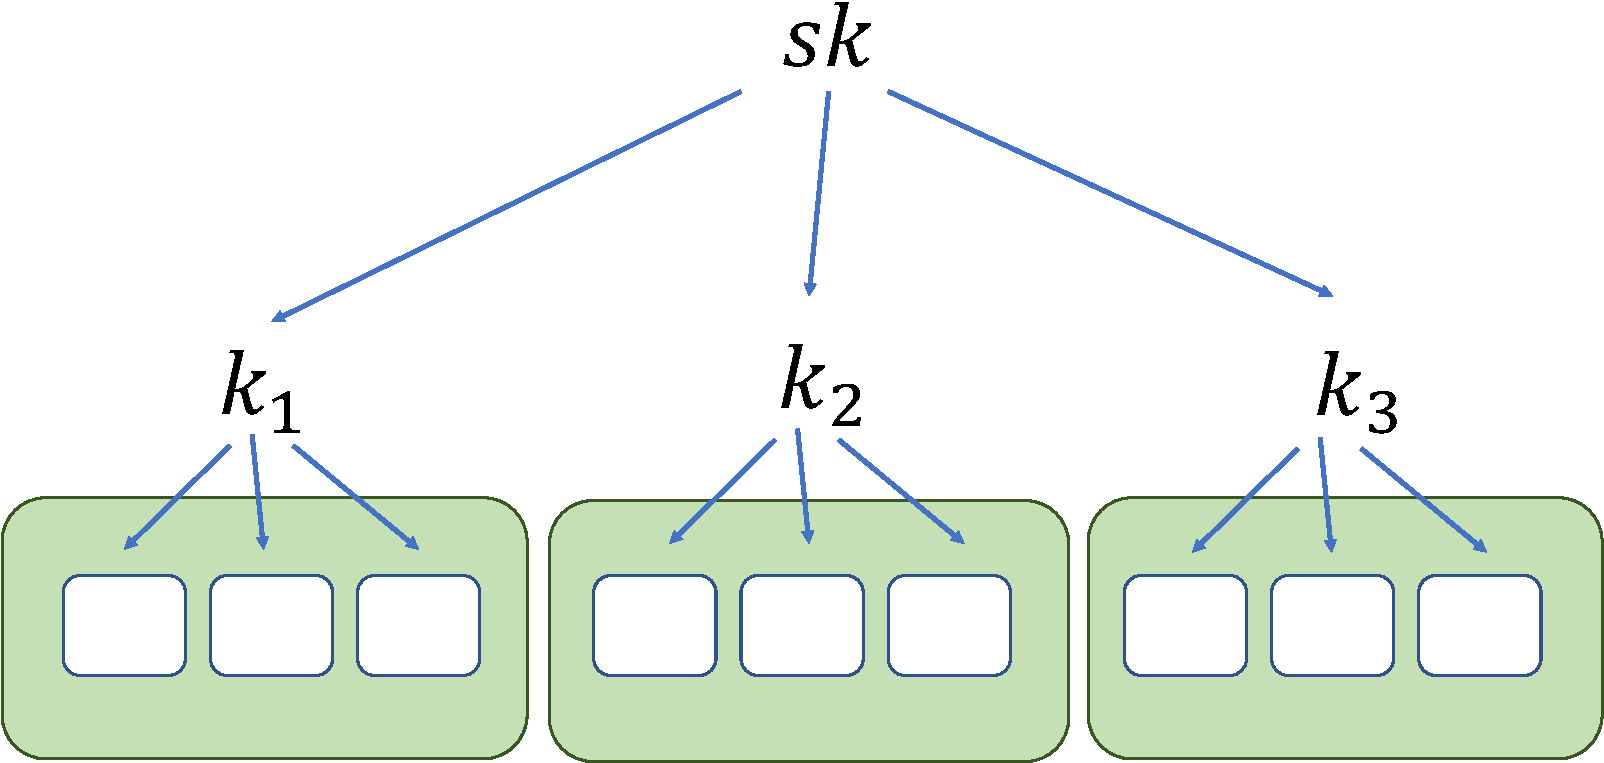
\includegraphics[width=0.5\linewidth]{figs/set-rep.pdf}
    \caption{Two-layer set representation\label{fig:set-rep}. The first layer key expands to $n^{1/4}$ superblock keys. Each superblock key further 
expands to $n^{1/4}$ offsets, one for each chunk in the superblock.}
\end{figure*}

\begin{figure*}[t]
    \centering
    \begin{subfigure}[t]{0.48\textwidth}
        \centering
        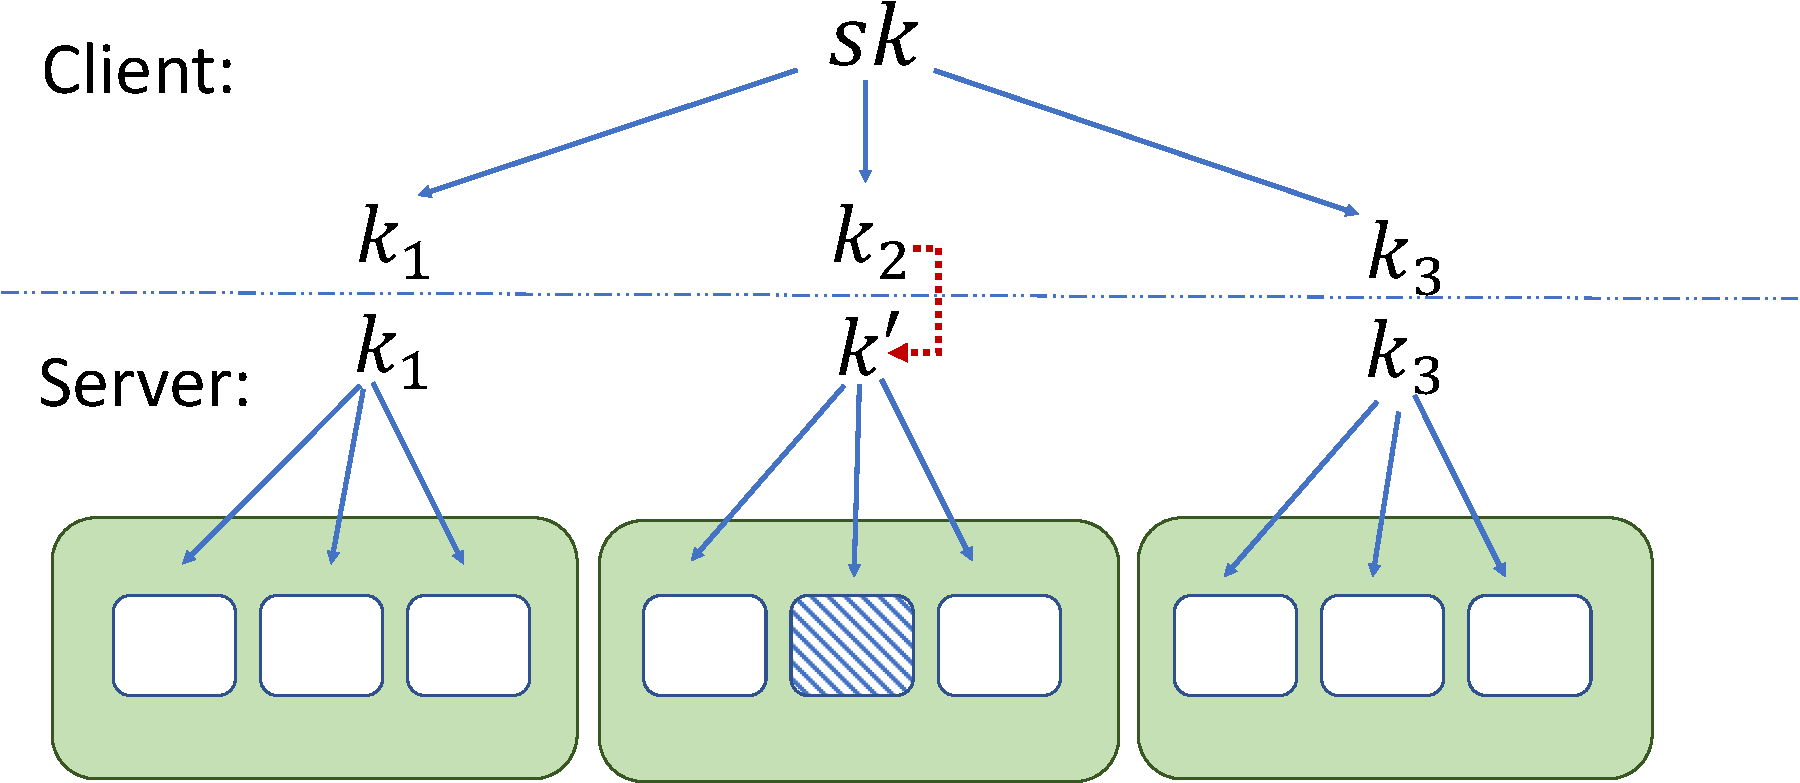
\includegraphics[width=\textwidth]{figs/step1.pdf}
        \caption*{Step 1: The client expands the \ppps key to $n^{1/4}$ superblock 
            keys and replaces the key corresponding to $x$'s superblock with a random key. 
        }\label{fig:step1}
    \end{subfigure}
    \hfill
    \begin{subfigure}[t]{0.48\textwidth}
        \centering
        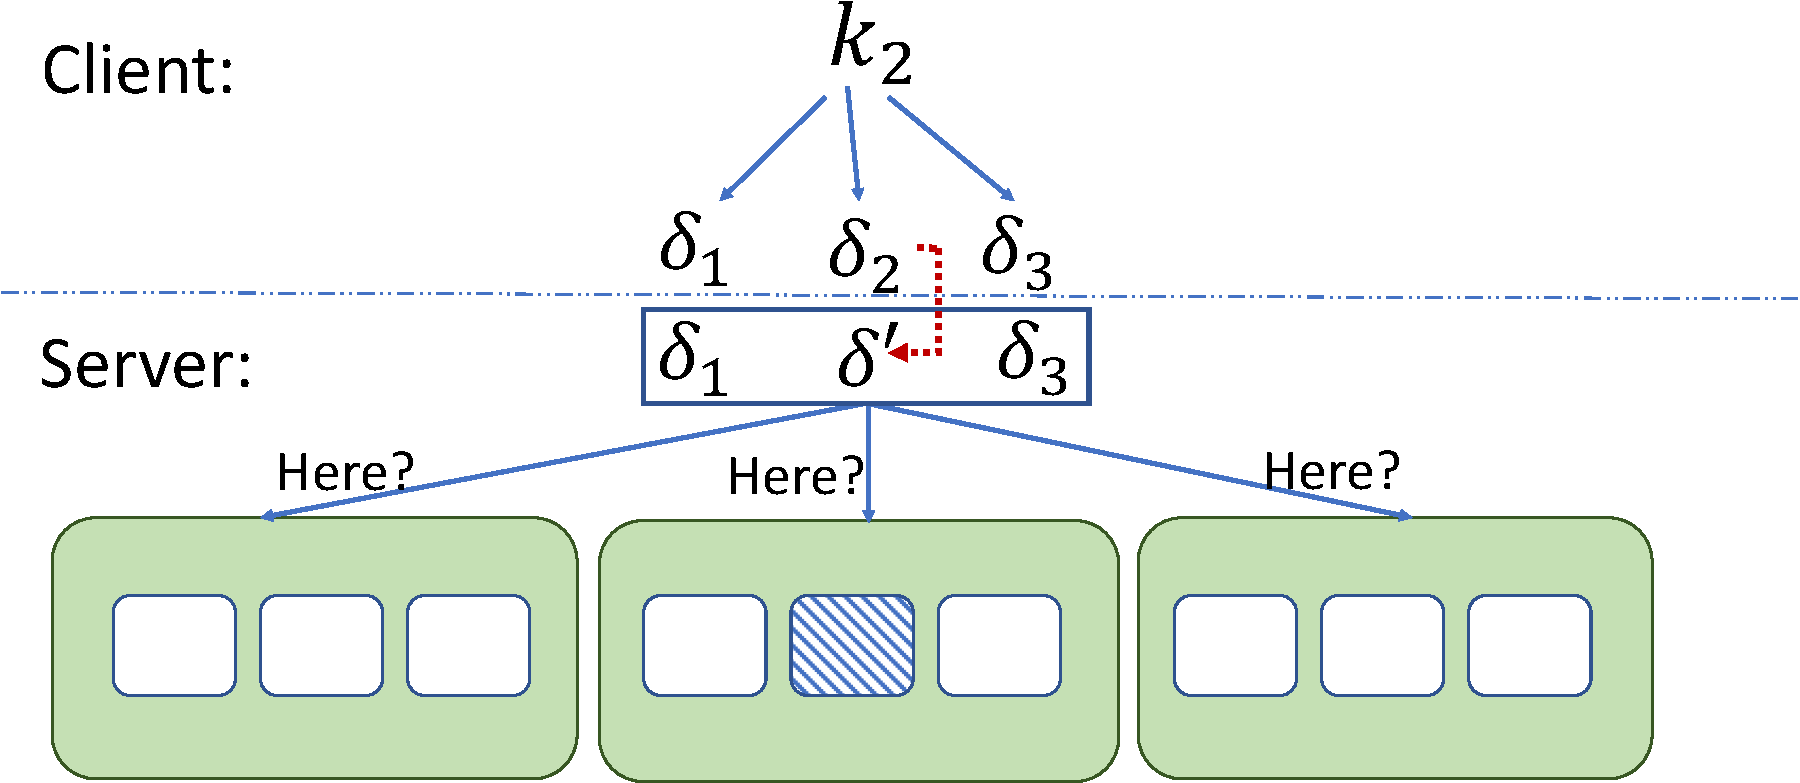
\includegraphics[width=\textwidth]{figs/step2.pdf}
        \caption*{Step 2: The client expands the 
            replaced superblock key to $n^{1/4}$ offsets and replaces $x$'s offset to a random one. 
            The server constructs the candidate sets by plugging these offsets into every superblock. 
        }
        \label{fig:step2}
    \end{subfigure}
    \caption{Illustration about how \ppps is used in our PIR schemes. The client programs the key and the server will decode the list of candidate sets.}
    \label{fig:algo}
\end{figure*}



\paragraph{Size of programmed key and efficiency of ${\sf ListDecode}$.}
Clearly, the programmed key $\sk'$ output by 
${\sf Program}$ has size $O_\lambda(n^{1/4})$.
It is also easy to have a succinct representation of
size $O(\sqrt{n})$ of all $n^{1/4}$ candidate sets output by 
${\sf ListDecode}$.
Specifically, one can first compute the common set $S$ of size $\sqrt{n}$ (we abuse the notation that this set is derived from flattening the matrix $S$ in $\ListDecode$). 
Then, the symmetric difference between the $i$-th candidate set and the common set $S$ is just $2n^{1/4}$ elements (those elements in the $i$-th superblocks). 
So the succinct representation (and hence the efficient algorithm) of $\ListDecode$ takes $O_\lambda(\sqrt{n})$ space and time.


%sets on

%can be recovered from the internal variable $S$ 
%in the ${\sf ListDecode}$ algorithm
%as well as $\{\delta^*_j\}_{j \in \{0, \ldots, %n^{1/4}-1\}}$.
\ignore{
We first write down the common set, $S$, as following:
\[
S=\{\delta_{i,j}+i\cdot n^{3/4} + j\cdot \sqrt{n} \}_{i,j\in \{0,\dots,n^{1/4}-1\}}
\] 
The key is that, the symmetric difference between the $i$-th decoded set $S_i$ and the common set $S$ only has $2n^{1/4}$ elements.
We just remove the elements in the $i$-th superblock and fill that superblock with the offsets of $\delta^*_0,\dots,\delta^*_{n^{1/4}-1}$. Specifically, its full description is:
\[
S_i = \left(S/\{ \delta_{i,j}+ i\cdot n^{3/4} + j\cdot \sqrt{n}\}_{j\in \{0,\dots,n^{1/4}-1\}}\right) \cup \left\{\delta^*_{j}+ i\cdot n^{3/4} + j\cdot \sqrt{n}\right\}_{ j\in \{0,\dots,n^{1/4}-1\}}
\]
This representation only takes $O(n^{1/4})$ extra space and time based on the representation of $S$. 
In total, we have $n^{1/4}$ possible sets.
We simply just store the common set $S$ (which takes $O(\sqrt{n})$ space and time) and store the difference between $S_i$ and $S$ for all $n^{1/4}$ possibilities (where each one takes $O(n^{1/4})$ space and time).
Then, the total time and space cost for $\ListDecode$ is just $O(\sqrt{n})$.
}

\paragraph{Efficient set membership.}
The above construction also supports
$O_\lambda(1)$-time set membership query. 
Given a secret key $\sk$ that has not been programmed, 
to check if some element $x \in {\sf Set}(\sk)$ or not, 
one simply has to check 
\[
\PRF_2(\PRF_1(\sk, \lfloor \ell/n^{1/4}\rfloor), \ \ \ell \text{ mod } n^{1/4}) 
\overset{?}{=} x \text{ mod } n^{1/2}
\text{ where } \ell = %{\sf chunk}(x)
\lfloor x/n^{1/2}\rfloor
\]


\subsection{Proof of Correctness}
To see correctness, 
let $\sk \leftarrow {\sf Gen}(1^\lambda, n)$, 
let $\sk', i^* \leftarrow {\sf Program}(\sk, \chunkid, \delta_\chunkid)$.
Recall that $\sk'$ can be parsed as 
$\sk' = (\{k_i\}_{i\in \{0, \ldots, n^{1/4}-1\}}, 
\{\delta^*_i\}_{i\in \{0, \ldots, n^{1/4}-1\}})$, 
and by construction, we know that 
$i^* = \lfloor \chunkid / n^{1/4}\rfloor$ is the index of the superblock 
that contains 
the chunk $\chunkid$.
Let $j^* := \chunkid \mod n^{1/4}$. 
Let $S_\emptyset := {\sf Set}(\sk)$, 
and we can view $S_{\emptyset}$
as a $n^{1/4} \times n^{1/4}$ matrix.
The correct programmed set $S^*$ is $S_\emptyset$
but replacing the element at index $(i^*, j^*)$
with $\delta_\chunkid$. %+ \chunkid \cdot \sqrt{n}$.

Below, we show that the set $S_i$ output by ${\sf ListDecode}$
is the same as $S^*$.
By %the definition of our algorithms, 
construction, 
in the ${\sf ListDecode}(\sk')$
algorithm, the intermediate set $S$ 
is the same as $S_{\emptyset}$
except for the $i^*$-th row.
Further, the $i^*$-th row of $S_\emptyset$
is the same as 
$\{\delta^*_j\}_{j\in \{0, \ldots, n^{1/4}-1\}}$
but replacing the $j^*$-th element
with $\delta_\chunkid$. %where $j^* := \chunkid \mod n^{1/4}$.
Additionally, the $S_i$ output 
by ${\sf ListDecode}$ is obtained by replacing
the $i^*$-th row of $S$ with 
$\{\delta^*_i\}_{i\in \{0, \ldots, n^{1/4}-1\}}$.




%where 
%$i$ is the superblock containing the $\chunkid$-th 
%chunk.




\subsection{Proof of Security}
We now prove pseudorandomness and private programmability
assuming the security of the underlying $\PRF_1$ and $\PRF_2$.

\paragraph{Pseudorandomness.}
Pseudorandomness follows directly from the pseudorandomness
of the underlying PRFs.

\paragraph{Private programmability.}
We can consider the following sequence of hybrid experiments.
Fix an arbitrary chunk identifier $\chunkid$
and an index $x$ that belongs to the $\chunkid$-th chunk.
Throughout, let $i^* = \lfloor \chunkid/n^{1/4} \rfloor$, let
$j^* = \chunkid \mod n^{1/4}$.

\paragraph{Experiment ${\sf Real}$.}
Recall the definition of the real experiment.
Sample a PRF key $\sk$ such that 
%$x \in {\sf Set}(\sk)$, 
$\PRF_2(\PRF_1(\sk, i^*), j^*) = x \mod \sqrt{n}$.
Let $\delta_\chunkid \getr \{0, 1, \ldots, \sqrt{n}-1\}$,  
and let $\sk', \_ \leftarrow {\sf Program}(\sk, \chunkid, \delta_\chunkid)$, 
output $\sk'$.

\paragraph{Experiment ${\sf Hyb}$.}
%Let $\delta_\chunkid \getr \{0, 1, \ldots, \sqrt{n}-1\}$.
Same as ${\sf Real}$ except with the following modification: 
when executing the ${\sf Program}(\sk, \chunkid, \delta_\chunkid)$ 
algorithm
instead of using the $k_0, \ldots, k_{n^{1/4}-1}$
keys that are expanded using $\PRF_1(\sk, \cdot)$, 
sample 
$k_0, \ldots, k_{n^{1/4}-1}$
at random subject to 
$\PRF_2(k_{i^*}, j^*) = x \mod \sqrt{n}$.

\begin{lemma}
Suppose that $\PRF_1$ is secure. 
Then, ${\sf Hyb}$ 
is computationally indistinguishable from ${\sf Real}$.
\label{lem:privateprog1}
\end{lemma}
\begin{proof}
%\elaine{FILL}
Suppose there is an efficient adversary $\mcal{A}$ that can distinguish
${\sf Real}$ and ${\sf Hyb}$ with non-negligible probability. 
We can construct the following efficient reduction 
$\mcal{B}$
which can distinguish a PRF from a random function 
with non-negligible probability. 
Basically, $\mcal{B}$ 
is interacting with its own challenger
who either answers queries using a PRF or using a truly random function.
$\mcal{B}$
will query its own challenger on the inputs 
$0, 1, \ldots, n^{1/4}-1$, 
and it will obtain 
$k_0, \ldots, k_{n^{1/4} - 1}$ from 
its challenger.
It will check if $k_{i^*}$
satisfies the relation 
$\PRF(k_{i^*}, j^*) = x \mod \sqrt{n}$. 
If not, $\mcal{B}$ aborts and outputs $0$. 
Otherwise, it runs the ${\sf Program}$ algorithm where it plugs in 
the terms $k_0, \ldots, k_{n^{1/4} - 1}$  
as the superblock keys.
It gives the resulting $\sk'$
to $\mcal{A}$. 
%Since the relationship 
%$\PRF(k_{i^*}, j^*) = x \mod \sqrt{n}$
Henceforth, we use $b = 0$ to denote the world  
in which $\mcal{B}$'s  challenger 
uses 
a truly random function, and we use $b = 1$ to denote
the world in which $\mcal{B}$'s challenger uses a randomly sampled PRF function.
We use the notation $\Pr_b[\cdot]$
to denote the probability of events in world $b \in \{0, 1\}$. 
Let $G$ be the good event that 
the relation 
$\PRF(k_{i^*}, j^*) = x \mod \sqrt{n}$
is satisfied.

\[
\Pr_b[\mcal{B} \text{ outputs } 1]
= 
0 \cdot \Pr_b [\overline{G}]
+ \Pr_b[ \mcal{A} \text{ outputs } 1 | G] \cdot \Pr_b[G]
\]

We know that $\Pr_0[G] = 1/\sqrt{n}$ which is non-negligible.
If the PRF is secure, then 
it must be that $|\Pr_1[G] - \Pr_0[G]| \leq \negl(\lambda)$
due to a straightforward reduction to PRF security.
Therefore, we have that 
\begin{align*}
 & \left|\Pr_1[\mcal{B} \text{ outputs } 1]
- \Pr_0[\mcal{B} \text{ outputs } 1]\right|\\
 = & 
\left| \Pr_1[ \mcal{A} \text{ outputs } 1 | G] \cdot \Pr_1[G]
- 
\Pr_0[ \mcal{A} \text{ outputs } 1 | G] \cdot \Pr_0[G]
\right|\\
\geq & 
\left|\Pr_1[ \mcal{A} \text{ outputs } 1 | G] 
- 
\Pr_0[ \mcal{A} \text{ outputs } 1 | G] \right|\cdot \frac{1}{\sqrt{n}}
- \negl(\lambda)
\end{align*}

Observe also that in world $0$, conditioned on $G$,
$\mcal{A}$'s view in the experiment is identically distributed
as ${\sf Hyb}$.  
In world $1$, conditioned on $G$,
$\mcal{A}$'s view in the experiment is identically distributed
as ${\sf Real}$.  
Therefore, the term 
\[\left|\Pr_1[ \mcal{A} \text{ outputs } 1 | G]
-
\Pr_0[ \mcal{A} \text{ outputs } 1 | G] \right|\]
represents $\mcal{A}$'s advantage
in distinguishing ${\sf Real}$ and ${\sf Hyb}$.
We can now conclude that if $\mcal{A}$ can distinguish
${\sf Real}$ and ${\sf Hyb}$ with non-negligible probability,
then $\mcal{B}$ can break PRF security with non-negligible probability.
\end{proof}


\paragraph{Experiment ${\sf Ideal}$.}
The ${\sf Ideal}$ experiment 
is almost the same as ${\sf Hyb}$ except with the following modification: 
when outputting the $\sk'$, 
instead of using the $\delta_0, 
\ldots, \delta_{j^*-1},  
\delta_{j^*+1},  
\delta_{n^{1/4}-1}$
terms derived from evaluating $\PRF_2(k_{i^*}, \cdot)$ 
at the points $0, 1, \ldots, j^*-1, j^*+1, \ldots, n^{1/4} -1$, 
we now sample $\delta_0,  
\ldots, \delta_{j^*-1},  
\delta_{j^*+1},  
\delta_{n^{1/4}-1}$
at random from $\{0, \ldots, n^{1/2}-1\}$ instead.

Observe that in the 
${\sf Ideal}$
experiment, we no longer make use of knowledge of the query $x$.
Therefore, %we can view the output 
the description of the ${\sf Ideal}$ 
experiment also uniquely specifies the simulator ${\sf Sim}$
we want to construct.

\begin{lemma}
Suppose that $\PRF_2$
is secure. Then, ${\sf Ideal}$ is computationally
indistinguishable from ${\sf Hyb}$.
\label{lem:privateprog2}
\end{lemma}
\begin{proof}
It suffices to show that the following to probability ensembles are
computationally indistinguishable
for any fixed $\delta^* \in \{0, 1, \ldots, \sqrt{n}-1\}$,
and $j^* \in \{0, 1, \ldots, n^{1/4} -1\}$.
\begin{enumerate}[leftmargin=5mm]
\item 
${\sf Distr_0}$:
Output a randomly sampled vector 
$\delta_0, \ldots, \delta_{n^{1/4}-1} 
\in \{0, 1, \ldots, \sqrt{n}-1\}^{n^{1/4}}$.
\item  
${\sf Distr_1}$:
Sample a PRF key $k$ subject to 
$\PRF_2(k, j^*) = \delta^*$.  
Sample $\delta' \in \{0, 1, \ldots, \sqrt{n}-1\}$ at random. 
For $j \in \{0, 1, \ldots, n^{1/4}-1\}$, 
compute $\delta_j = \PRF_2(k, j)$.
Output 
$\delta_0, \ldots, \delta_{j^*-1}, \delta', 
\delta_{j^*+1}, \ldots, \delta_{n^{1/4}-1}$.
\end{enumerate}

If there is an efficient adversary $\mcal{A}$ that can distinguish
between the above 
${\sf Distr}_0$ 
and  
${\sf Distr}_1$ 
with non-negligible probability, we can construct an efficient 
reduction $\mcal{B}$
that can distinguish
whether it is interacting with a random oracle 
or a randomly chosen PRF function.
Basically, $\mcal{B}$ 
sends the inputs $0, \ldots, n^{1/4}-1$ to the oracle 
it is interacting with, and gets back
$\delta_0, \ldots, \delta_{n^{1/4}-1}$.
If $\delta_{j^*} \neq \delta^*$, 
then $\mcal{B}$ aborts and outputs $0$. 
Otherwise, it 
replaces $\delta_{j^*}$ with a random value
from $\{0, \ldots, n^{1/2}-1\}$
and gives the resulting vector to $\mcal{A}$.
Suppose $\mcal{B}$ is interacting with a random oracle,
then conditioned on the good event 
$\delta_{j^*} = \delta^*$, $\mcal{A}$'s view
is identically distributed as ${\sf Distr}_0$.
On the other hand, suppose $\mcal{B}$ is interacting with a PRF,
then conditioned on the good event 
$\delta_{j^*} = \delta^*$, $\mcal{A}$'s view
is identically distributed as ${\sf Distr}_1$.
The rest of the proof can be completed due
to a similar probability calculation as 
\Cref{lem:privateprog1}.
\end{proof}








\section{Our Two-Server PIR Scheme}\label{sec:two-server}

\begin{figure}[p]
    \begin{minipage}{\textwidth}
        \begin{mdframed}
            \label{alg:one-query-ppwps-two}
            \begin{center}
                {\bf Two-server scheme for $Q = \sqrt{n} \log \kappa \cdot \alpha$ queries}
            \end{center}

            \parhead{Offline preprocessing.} 
            %\ \\[-6pt]
%{\it Client}:
            \begin{itemize}[leftmargin=3mm,itemsep=1pt,topsep=1pt]
            %    \item 
                            %, where $M_1=\sqrt{n}\log \kappa \cdot \alpha(\kappa)$. , such
                %that $\alpha(n)=\omega(1)$. 
                % Initialize the parities $p_1,\dots,p_{M_1}$ to zeros.
                
                
                \item 
{\it Hint table.}
Let $M_1=\sqrt{n}\log \kappa \cdot \alpha(\kappa)$. For each $i\in [M_1]$, 
sample a fresh \ppps key $\sk_i$, 
send $\sk_i$ 
to the \underline{right server} 
and receive a parity $p_i := \oplus_{j \in \Set(\sk_i)} \DB[j]$ back. 
%and receive their parities $p_1,\ldots,p_{M_1}$. 
Let $T := \{(\psk_i, p_i )\}_{i \in
                [M_1]}$ denote the client's {\it hint table}.
                \item 
{\it Replacement entries.}
For each chunk $\ell \in \{0,\ldots,\sqrt{n}-1\}$,
repeat the following 
$M_2=3\log \kappa \cdot \alpha(\kappa)$  times:
sample a random index $r_1 \in \{0, \ldots, n-1\}$ in chunk $\ell$, 
send $r_1$ to the \underline{left server}, and receive $\DB[r_1]$.
Store the tuple $(r_1,\DB[r_1])$. 

Similarly, 
for each chunk $\ell \in \{0,\ldots,\sqrt{n}-1\}$,
repeat the following $M_2$  times:
sample a random index $r_2$ in chunk $\ell$, 
send $r_2$ to the \underline{right server}, and receive $\DB[r_2]$.
Store the tuple $(r_2,\DB[r_2])$. 
            \end{itemize}

%\vspace{5pt}
%{\it Right server}:
%upon receiving a \ppps key $\sk$, return $\oplus_{i \in \Set(\sk)}\DB[i]$.

            
            \parhead{Query for index $x \in \{0, 1, \ldots, n-1\}$.}
            
            \begin{enumerate}[leftmargin=5mm,itemsep=1pt]
                \item 
                {\bf Step 1: (Client Querying)}

                \begin{itemize}[leftmargin=5mm,itemsep=1pt]
                        \item Find the first entry $(\sk,p)$ in the hint table such that $x\in \Set(\sk)$.~\footnote{
In a rare case, if not found, let $\sk$ be a freshly sampled \ppps key subject
to $x \in \Set(\sk)$, 
and let $p = 0$.}
\item 
Find the first unconsumed 
replacement entries  
$(r_1, \DB[r_1])$ retrieved from right server,
such that $r_1$ is in $\chunk(x)$.
\footnote{In a rare case, if such an $r_1$ is not found, let it be a random
index in $\chunk(x)$, and use $0$ whenever $\DB[r_1]$ is needed later.} 
                        \item $(\sk_1',j_1)\gets\Program(\sk,\chunk(x),r_1\text{ mod } \sqrt{n})$.
                        \item 
                        Send $\sk'_1$ to the left server.     
                \end{itemize}

                \item
               {\bf Step 2: (Client Reconstructing)}
               \begin{itemize}[leftmargin=5mm,itemsep=1pt]
                   \item Receive $(\beta_{0,1},\ldots,\beta_{n^{1/4}-1,1})$ from the left server.
                   \item Save the answer as $y=p\xor  \DB[r_1]\xor\beta_{j_1,1}$.
               \end{itemize}
               
                \item
               {\bf Step 3: (Client Refreshing)}
               \begin{itemize}[leftmargin=5mm,itemsep=1pt]
                   
                   \item Sample $\sk_2$ such that $x\in\Set(\sk_2)$.
                   \item 
                   Find the first unconsumed 
                   replacement entries  
                   $(r_2, \DB[r_2])$ retrieved from left server, 
                   such that $r_2$ is in $\chunk(x)$.
                   \item $(\sk_2',j_2)\gets\Program(\sk_2,\chunk(x),r_2\text{ mod } \sqrt{n})$. 
                   \item Send $\sk_2'$ to right server.
                   \item Receive $(\beta_{0,2},\ldots,\beta_{n^{1/4}-1,2})$
                   from the right server.        
                   \item Replace the hint $(\sk,p)$ with $(\sk_2,\DB[r_2]\xor \beta_{j_2,2}\xor y)$ in the table.
               \end{itemize}
               
               \item 
               {\bf Server Responding: (Same for Left and Right Server)}
               \begin{itemize}[leftmargin=5mm,itemsep=1pt]
                   \item  Upon receiving $\sk'$, compute $(S_0,S_1,\ldots,S_{n^{1/4}-1})\gets \ListDecode(\sk')$.
                   \item Return $(\beta_0,\dots,\beta_{n^{1/4}-1})$ to the client where $\beta_i=\oplus_{i\in S_b}\DB[i]$.
               \end{itemize} %\hfill {\it // $L= n^{1/4}$}
               
            \end{enumerate}
        \end{mdframed}
    \end{minipage}
    \caption{Two-server preprocessing PIR with ${O}_\lambda(n^{1/4})$ communication, ${O}_\lambda(n^{1/2})$ computation based on PRFs. 
    }
    \label{fig:2server-new}
\end{figure}





\subsection{Construction}

\paragraph{Intuition.} 
The scheme has three major components.
\begin{itemize}[leftmargin=*]
    \item \textit{Preprocessing.} The client randomly samples $\tilde{O}(\sqrt{n})$ privately programmable pseudorandom sets, each of size $\sqrt{n}$. 
    It queries the \underline{right server} for the sets' parities, storing them along with the keys.
    Moreover, the client queries the \underline{right server} for the values of logarithmic numbers of randomly sampled indices for each $\sqrt{n}$-size chunk.
    Those entries are stored as the ``replacement'' entries.
    
    \item \textit{Online Query.} 
    Given a query $x$, the client finds a set $S$ such that $x\in S$.
    The client then finds a replacement entry $r$ that resides in the same chunk as $x$. 
    The client privately programs the set, intending to change it from $S$ to $(S/\{x\})\cup \{r\}$.
    Once the client knows the parity for this new set, it can compute $\DB[x]$ because it already knows $\DB[r]$ and the parity for $S$.
    The client uses the PPPS programming function to program the set, and sends the programmed key $\sk'$ to the \underline{left server}.
    The \textit{left server} runs the list decoding algorithm, then computes and returns all $n^{1/4}$ candidate sets' parities.
    The client knows that there is one candidate parity corresponding to the correct set $(S/\{x\})\cup \{r\}$, which is enough to compute the answer.
    
    \item \textit{Refresh.} 
    Each query consumes a set. %The client needs to replace the consumed set with a new set.
    After each query, the client just samples a new set conditioned on it containing the query $x$, and queries the \textit{right server} for its parity with the same query technique mentioned above. 
    The new set will replace the consumed set.
\end{itemize}

\ignore{
\paragraph{Intuition of the PIR scheme based on PPPS.} 
During the preprocessing phase, the client randomly samples $M_1=\tilde{O}(\sqrt{n})$ privately programmable pseudorandom sets, whose keys are denoted as $\sk_1\dots,\sk_{M_1}$, and queries the \textit{right server} for the parities for all these sets, denoted as $p_1,\dots,p_{M_1}$.
Moreover, the client queries the \textit{right server} for $M_2=\tilde{O}(1)$ random ``replacement'' entries for each $\sqrt{n}$-size chunk, and stores their indices and values as the form of $(r,\DB[r])$.
During the online phase, given a query $x$, the client finds a key $\sk$ that $\Set(\sk)$ contains $x$. The set's parity is denoted as $p$.
The client then finds a replacement entry $r$ that is in the same chunk as $x$, and it privately programs the set, intending to change it from $\Set(\sk)$ to $(\Set(\sk)/\{x\})\cup \{r\}$.
Once the client knows the parity for this new set, it can computes $\DB[x]$ because it already knows $\DB[r]$ and the parity for $\Set(\sk)$.
Specifically, the client programs the offset of $r$ in $\chunk(x)$ to the key $\sk$ using the PPPS programming function, and sends the programmed key $\sk'$ to the \textit{left server}.
The \textit{left server} runs the list decoding algorithm, then computes and returns all $n^{1/4}$ candidate sets' parities.
The client knows that there is one candidate parity corresponding to the correct set $(\Set(\sk)/\{x\})\cup \{r\}$ and it is enough to compute the answer.
To support multiple queries, the client needs to replace the consumed key with a new one.
After each query, the client just samples a new PPPS key conditioned on its set containing the query $x$, and queries the \textit{right server} for the parity for this new set with the same private query technique mentioned above. 
The client will replace the consumed key with this new key.
}

\paragraph{Detailed algorithm for bounded, random queries.}
We describe the detailed construction
for $Q = \sqrt{n} \log \kappa \cdot \alpha$ random, distinct queries 
in \Cref{fig:2server-new}.
We can easily extend such a scheme to support
unbounded, arbitrary queries using known techniques~\cite{pir-ec23}. 
For completeness, we explain how the extension works shortly after.



\paragraph{Efficiency.}
Observe that the list decoding
produces $n^{1/4}$ candidate sets
each of size $\sqrt{n}$.
Naively, expanding all sets and computing their corresponding parities takes $O_\lambda(n^{3/4})$ time.
We are still going to rely on the fact that $\ListDecode$ has an $O(\sqrt{n})$-size succinct representation to optimize the computation. 
Recall that we can first compute the common set of size $\sqrt{n}$, and then the symmetric difference between each possible decoding set and the common set will only contain $2n^{1/4}$ elements. 
Therefore, to compute the parities for all $n^{1/4}$ possible sets, we first compute the parity for the common set $S$, which takes $O_\lambda(\sqrt{n})$ time.
Then, it takes $O_\lambda(n^{1/4})$ time to enumerate the symmetric difference between the $i$-th set and the common set, which suffices to compute the parity for the $i$-th set.
So the total computation time will be $O_\lambda(\sqrt{n})$.

\paragraph{Supporting unbounded, arbitrary queries.}
For completeness, we review the techniques described in previous works 
for upgrading the scheme for $Q$ random, distinct queries to a scheme
supporting unbounded, arbitrary queries.
We can easily get rid of the distinct query
assumption in the following way: we require the client to store a local cache of size $Q$ for caching the
most recent $Q$ queries. If the client wants a repeated query, it can lookup
in the cache and make a distinct fake query. 

Further, we can assume that the queries are random without loss of generality as follows: 
we can let the client and the servers agree on 
a small-domain pseudorandom permutation (PRP)~\cite{prp1,prp2} 
(which is implied by one-way functions~\cite{swapornot})
upfront and the server can permute the database according to the PRP. 
Another option is let one of the servers
build the database as a key-value storage and use a cuckoo hash
table~\cite{cuckoo1,cuckoo2} directly based on a PRF to locate the queries, and share it with the other server.
Notice that, in both implementations, the client can still make queries
adaptively depending on the real query sequence and the responses, which is
sufficient for practical usage. Then, as long as the client makes the
queries independent of the randomness of the PRP/PRF, those queries can be
considered as uniformly random. This assumption is only needed for the
correctness.

Lastly, we can remove the bounded $Q$ query assumption as follows: 
we use a pipelining trick suggested in earlier works~\cite{pir-ec23,piano}. 
Essentially, we can spread the pre-processing for the next window of $Q$ queries
over the current window of $Q$ queries.
\ignore{
The scheme first runs a preprocessing phase for the first $Q$ queries. 
Then, during the query phase, the client interacts with the preprocessing server and gradually finishes the preprocessing for the next $Q$ queries. 
Essentially, the client and the server can split the work (including computation and communication) of the preprocessing into $Q$ pieces.
Whenever the client finishes a query, the client and the preprocessing server will finish the next piece of work about preprocessing.
Once the client finishes the $Q$ queries, it can immediately start the next window of $Q$ queries because the preprocessing for the next window is done. 
As stated above, the preprocessing phase needs ${O}_\lambda(\sqrt{n})$ communication and ${O}_\lambda(n)$ in total.  Thus, in our final scheme, we have a one-time preprocessing phase with ${O}_\lambda(n)$ communication, ${O}_\lambda(n)$ computation, while consuming only ${O}(\sqrt{n})$ client storage. After the one-time preprocessing,
we can support an unbounded number of arbitrary queries. The communication and computation
cost of each query is ${O}_\lambda({n}^{1/4})$ and the computation cost of each query is ${O}_\lambda(\sqrt{n})$.
}






\begin{theorem}
    \label{thm:eff2srv} %Let $\lambda,\kappa\in \mathbb{N}$.
    Let $\alpha(\kappa)$ be any superconstant function. 
Suppose that $\PRF_1,\PRF_2$ are secure pseudorandom functions, and that 
$n$ is bounded by $\poly(\lambda)$ and
    $\poly(\kappa)$. The two-server scheme in~\Cref{fig:2server-new} 
that supports
    $Q = \sqrt{n}\log \kappa \cdot \alpha$ 
random, distinct
queries is private, and correct with probability
    $1-\negl(\lambda)-\negl(\kappa)$ for some negligible function 
$\negl(.)$. Further, it achieves the following performance
    bounds:
    \begin{itemize}
        \item $O_\lambda(\sqrt{n}\log \kappa \alpha(\kappa))$ client storage and
        no additional server storage;
        \item \textbf{Pre-processing Phase}:
        \begin{itemize}
            \item $O_\lambda(n \log \kappa \cdot \alpha)$ 
server time and $O_\lambda(\sqrt{n}\log \kappa \cdot \alpha)$ client time;
            \item $O_\lambda(\sqrt{n} \log \kappa \cdot \alpha)$ communication;
        \end{itemize}
        \item \textbf{Query Phase}:
        \begin{itemize}
            \item 
$O_\lambda(\sqrt{n})$ expected client time 
and $O_\lambda(\sqrt{n})$ server
            time per query; 
            \item $O_\lambda(n^{1/4})$
            communication per query.
        \end{itemize}
    \end{itemize} 
Therefore, the amortized communication per query
is %\elaine{FILL}  
$O_\lambda(n^{1/4})$, and the amortized server computation
and expected client computation
per query is %$O_\lambda(\sqrt{n}\log \kappa \cdot \alpha)$, 
$O_\lambda(\sqrt{n})$.
\end{theorem}
\begin{proof}
We defer the privacy and correctness proofs to \Cref{sec:2server-priv}
and \Cref{sec:2server-correct}
respectively. Here, we focus on proving the efficiency claims.

The client stores $M_1 = \sqrt{n} \log \kappa \cdot \alpha$ number
of \ppps keys, and $M_2 = 3 \log \kappa \cdot \alpha$ number
of replacement entries per chunk.
Therefore, the space required is $O_\lambda(\sqrt{n} \log \kappa \cdot \alpha)$.

During the offline phase, the client
sends $M_1$ \ppps  
keys to the right server, and sends $M_2$ indices per chunk
to either server for constructing replacement entries.
Therefore, the offline communication is bounded
by $O_\lambda(\sqrt{n} \log \kappa \cdot \alpha)$. 
The right server needs to expand the sets for each \ppps key received
and evaluate the xor-sums.  
Both servers need to return the bits for the replacement entries.
Therefore, the total server computation is bounded
by $O_\lambda(n \log\kappa \cdot \alpha)$.

During the query phase, the client
sends one programmed \ppps key to each server,
and the size of a programmed key is at most $O_\lambda(n^{1/4})$.
Each server sends back the xor-sums of $n^{1/4}$
candidate sets.
Each candidate set has size $n^{1/2}$, however, all
$n^{1/4}$ candidate sets has a succinct representation
of size only $n^{1/2}$, 
and server can compute this succinct representation
in time $O_\lambda(n^{1/2})$.
Further, it is not hard to see that due to the structure
of the candidate sets, the server can compute
all $n^{1/4}$ xor-sums in time only $O(n^{1/2})$.
Therefore, the servers' running time is
bounded by $O_\lambda(n^{1/2})$
during each query query.
The client needs to find a matched hint, and compute
$O(1)$ xor operations during each query.
Its running time is 
dominated by the cost of finding a matched hint, which
can be done by invoking the set membership operation
for each of the $M_1$ hints.
Using \Cref{lem:2server-hintfresh}
and the pseudorandomness property of the \ppps, the expected
number of hints checked until a key $\sk$ such that $\Set(\sk)$ contains the current query is found is $O(\sqrt{n})$.
The expected number of tries till success is $\sqrt{n}$.
Therefore, the client's expected running time per query
is upper bounded by $O_\lambda(\sqrt{n})$.
\end{proof}



\subsection{Privacy Proof}
\label{sec:2server-priv}

Suppose that the underlying \ppps scheme satisfies
private programmability.
Below, we prove the privacy of our two-server PIR scheme.

In the pre-processing 
phase, the server sends the sets $\Set(\sk_i)$ only to the right server, thereby no information about these sets is leaked to the left server. Similarly, no information about the indices $r_1$ is leaked to the right server and no information about the indices $r_2$ is leaked to the left server.
We will first the lemma about the distribution of client's hint table, when the adversary controls either of the left or right server.
\begin{lemma}
 Recall that in each time step $t$, the adversary \algA 
adaptively chooses a query $x_t \in \{0, 1, \ldots, n-1\}$ for the client.
%The following statements are true:
%\begin{enumerate}[leftmargin=5mm]
%\item 
At the end of each time step $t$, 
the client's hint table  
is distributed 
as a table of size $M_1$
where each entry is a freshly sampled \ppps key, even when
conditioned on $\algA$'s view so far.  
%\end{enumerate}
\label{lem:2server-hintfresh}
\end{lemma}
\begin{proof}
Suppose the above statement holds at the end of time step $t-1$.
We prove that it still holds 
at the end of time step $t$.
Since the hint table is distributed as a fresh randomly sampled
table even when conditioned on $\algA$'s view
at the end of $t-1$, we may henceforth assume
an arbitrary fixed query $x_t$.
The distribution of the hint table 
before the $t$-th query can be equivalently rewritten as:
\begin{itemize}[leftmargin=5mm]
\item First, 
sample the decision whether any 
of the $M_1$ entries contains the current query $x_t$,
and if so, which is the first entry (denoted $i^*$) 
that contains $x_t$. 
If not found, we assume $i^* = M_1 + 1$. 
\item 
For each $i < i^*$, sample a random \ppps
key subject to not containing $x_t$.
\item 
For each $i = i^*$, sample a random \ppps
key subject to containing $x_t$.
\item 
For each $i > i^*$, sample a random \ppps key.
\end{itemize}

Using the above interpretation, it is easy to see 
that the distribution of the hint table 
after the $t$-th query is unaltered 
no matter which of the two servers \algA controls.
\end{proof}


\subsubsection{Left Server Privacy}
We first construct 
the following simulator for proving left server privacy.

\paragraph{Simulator construction.}
\begin{itemize}[leftmargin=5mm]
\item  
During the pre-processing phase, 
for each chunk $\ell$, sample $M_2$ 
random indices belonging to $\ell$, send them to $\algA$.
\item 
During each query, 
call the simulator of the \ppps scheme which outputs $\sk'$, 
send $\sk'$ to $\algA$. 
\end{itemize}

\paragraph{Indistinguishability of ${\sf Real}$ and ${\sf Ideal}$.}
We now prove the indistinguishability of the ${\sf Real}$ and
${\sf Ideal}$ for both the servers
assuming the 
private programmability of the underlying \ppps scheme.

First, due to \Cref{lem:2server-hintfresh}, 
we can equivalently rewrite the ${\sf Real}$ experiment 
for the right server as follows:
at the end of each time step, resample the entire hint table
freshly at random before continuing to answer more queries.
As a result, 
the view of $\algA$ who controls the right server is 
distributed as: 
\begin{itemize}[leftmargin=5mm]
\item {\it Pre-processing phase}.
%Sample $M_1$ random \ppps keys, and send them to $\algA$. 
For each chunk $\ell$, send $M_2$ random indices
in chunk $\ell$ to \algA.
\item {\it Each time step $t$}.
\begin{itemize}[leftmargin=5mm]
\item 
sample a \ppps key $\sk$
 at random subject to containing the query $x_t$;
sample $\delta$ at random
from $\{0, \ldots, \sqrt{n}-1\}$.
\item 
call $\sk', \_ \leftarrow {\sf Program}(\sk, \chunk(x_t), \delta)$; 
\item 
send $\sk'$ to \algA.
\end{itemize}
\end{itemize}
One way to see this is to think of the distribution of the table
as the equivalent distribution
in the proof of \Cref{lem:hintfresh}. 
Further, observe that each $r_2\text{ mod }\sqrt{n}$ in the scheme 
is distributed randomly from the perspective
of the left server,  
since they 
were only sent to the 
right server during the pre-processing phase.
%because the right server has no information about $r_1$ during preprocessing.
%For the right server, the distribution of $\sk'$ is the actual distribution and $r_1\text{ mod }\sqrt{n}$ is distributed randomly because the right server has no information about $r_2$ during preprocessing.

Therefore, the rest of the proof follows
due to a straightforward hybrid argument
where we replace
the programmed keys (denoted $\sk'$ earlier) 
sent to the right server in all time steps one by one
with a simulated key, 
relying on the private programmability of the underlying \ppps. 






\subsubsection{Right Server Privacy}

We first construct 
the following simulator for proving right server privacy.

\paragraph{Simulator construction.}
\begin{itemize}[leftmargin=5mm]
\item  
During the pre-processing phase, 
send $M_1$ randomly sampled \ppps keys to $\algA$.
Further, for each chunk $\ell$, sample $M_2$ 
random indices in $\ell$, send them to $\algA$.
\item 
During each query, 
call the simulator of the \ppps scheme which outputs $\sk'$, 
%sample a random \ppps key $\sk$ subject to containing $x_t$, 
%sample a random $\delta \in \{0, \ldots, \sqrt{n}-1\}$, 
%call $\sk',\_ \leftarrow {\sf Program}(\sk, 
%\chunk(x_t), \delta)$, 
send $\sk'$ to $\algA$. 
\end{itemize}


\paragraph{Indistinguishability of ${\sf Real}$ and ${\sf Ideal}$.}
We now prove the indistinguishability of the ${\sf Real}$ and
${\sf Ideal}$ for both the servers
assuming the 
private programmability of the underlying \ppps scheme.
\ignore{
First, due to \Cref{lem:2server-hintfresh}, 
we can equivalently rewrite the ${\sf Real}$ experiment 
for the right server as follows:
at the end of each time step, resample the entire hint table
freshly at random before continuing to answer more queries.
As a result, 
}
The view of $\algA$ who controls the right server is 
distributed as: 
\begin{itemize}[leftmargin=5mm]
\item {\it Pre-processing phase}.
Sample $M_1$ random \ppps keys, and send them to $\algA$. 
Further, for each chunk $\ell$, send $M_2$ random indices
in chunk $\ell$ to \algA.
\item {\it Each time step $t$}.
\begin{itemize}[leftmargin=5mm]
\item 
sample a \ppps key $\sk$
 at random subject to containing the query $x_t$;
sample $\delta$ at random
from $\{0, \ldots, \sqrt{n}-1\}$.
\item 
call $\sk', \_ \leftarrow {\sf Program}(\sk, \chunk(x_t), \delta)$; 
\item 
send $\sk'$ to \algA.
\end{itemize}
\end{itemize}
%One way to see this is to think of the distribution of the table
%as the equivalent distribution
%in the proof of \Cref{lem:hintfresh}. 
To see the above, observe that each 
$r_1\text{ mod }\sqrt{n}$ in the scheme 
is distributed randomly from the perspective
of the right server,  
since they 
were only sent to the 
left server during the pre-processing phase.
%because the right server has no information about $r_1$ during preprocessing.
%For the right server, the distribution of $\sk'$ is the actual distribution and $r_1\text{ mod }\sqrt{n}$ is distributed randomly because the right server has no information about $r_2$ during preprocessing.

Therefore, the rest of the proof follows
due to a straightforward hybrid argument
where we replace
the programmed keys (denoted $\sk'$ earlier) 
sent to the right server in all time steps one by one
with a simulated key, 
relying on the private programmability of the underlying \ppps. 




\ignore{
\paragraph{Simulator construction and the ${\sf Ideal}$ experiment.}
Consider the following simulator construction for both the left server which does not make
use of the queries: 
in every time step $t$, call the simulator $\Sim$ of the \ppps
scheme, and let the output be $\sk'$. 
Send $\sk'$ to the server. 

\paragraph{Indistinguishability of ${\sf Real}$ and 
${\sf Ideal}$.}
We now prove the indistinguishability of the ${\sf Real}$ and
${\sf Ideal}$ for both the servers
assuming the 
private programmability of the underlying \ppps scheme.

First, due to \Cref{lem:hintfresh}, 
we can equivalently rewrite the ${\sf Real}$ experiment for the left and te right server as follows:
at the end of each time step, resample the entire hint table
freshly at random before continuing to answer more queries.
As a result, the %distribution of the $\sk'$ received by 
messages sent to 
\algA in each time step $t$
is distributed as 
\begin{itemize}[leftmargin=5mm]
\item[]
\begin{itemize}[leftmargin=5mm]
\item 
sample a \ppps key $\sk$
 at random subject to containing the query $x_t$;
sample $\delta$ at random
from $\{0, \ldots, \sqrt{n}-1\}$.
\item 
call $\sk', \_ \leftarrow {\sf Program}(\sk, \chunk(x_t), \delta)$; 
\item 
send $\sk'$ to \algA.
\end{itemize}
\end{itemize}
One way to see this for the left server is to think of the distribution of the table
as the equivalent distribution
in the proof of \Cref{lem:hintfresh}. Moreover, $r_1\text{ mod }\sqrt{n}$ is distributed randomly because the right server has no information about $r_1$ during preprocessing.
For the right server, the distribution of $\sk'$ is the actual distribution and $r_1\text{ mod }\sqrt{n}$ is distributed randomly because the right server has no information about $r_2$ during preprocessing.

Therefore, the rest of the proof follows
due to a straightforward hybrid argument
where we replace
the programmed keys (denoted $\sk'$ earlier) 
sent to the server in all time steps one by one
with a simulated key, 
relying on the private programmability of the underlying \ppps. 
}


\subsection{Correctness Proof}
\label{sec:2server-correct}

We show that with $Q = \sqrt{n} \log \kappa \cdot \alpha$ 
random, distinct queries,
the probability of ever having correctness error is negligibly small. 
An error can happen 
if one of the following bad events take place:
\begin{itemize}[leftmargin=5mm]
\item 
{\it No matched hint}. 
During some query for $x$, 
no hint is found that contains the query $x$.
\item 
{\it Depleting replacement entries}. 
During some query for $x$, there is no more replacement
entry of the form $(r_1, \DB[r_1])$ 
or $(r_2, \DB[r_2])$ 
corresponding to $\chunk(x)$. 
\end{itemize}

Below, we show 
that the probability of each bad event during a window
of $Q$ random, distinct queries 
is negligibly small. 

\paragraph{Probability of no matched hint.}
Due to \Cref{lem:2server-hintfresh}, for any fixed time step $t$, 
we can assume the client's hint table
contains freshly sampled \ppps keys and is independent of 
the current query $x_t$.
Due to the pseudorandomness property of the \ppps,
the sets generated by the keys 
in the hint table are computationally indisintinguishable
from 
$M_1$ sets independently sampled from the distribution $\mcal{D}_n$.
Below we 
calculate the probability that a fixed  
element $x_t$ is not in any of the $M_1$ sets 
sampled independently from 
$\mcal{D}_n$ --- the probability that $x_t$ is not contained in any entry in the
client's hint table can only be negligibly different.

The probability that one set 
sampled from $\mcal{D}_n$ contains $x_t$ is $1/\sqrt{n}$. 
Therefore, the probability that 
none of the $M_1$ sets contains $x_t$ is
$(1-1/\sqrt{n})^{M_1}$, and given the choice
of $M_1 = \sqrt{n} \log \kappa \alpha(\kappa)$ where $\alpha(\kappa)$
is a super-constant function,
this probability is negligibly small in $\kappa$.

Finally, taking a union bound over all polynomially many time steps,
the probability of ever not having a matched hint
is negligibly small in $\kappa$. 


\paragraph{Probability of depleting replacement entries.} 
One can only deplete the replacement 
entries of some chunk $\ell$ if the chunk $\ell$
is encountered more than $M_2$ times.
With $Q$ random distinct queries, 
each query will hit a random chunk.
The expected number of hits per chunk
is therefore $Q/\sqrt{n} = \log \kappa \cdot \alpha$.
By the Chernoff bound, 
the probability that the number of visits to some fixed chunk $\ell$
exceeds $M_2 = 3 \log \kappa \cdot \alpha$ is negligibly small
in $\kappa$ as long as $\alpha(\kappa)$ is a super-constant function.

Finally, taking a union bound over 
all chunks and 
all polynomially many time steps,
the probability of ever 
depleting replacement entries of any chunk
is negligibly small in $\kappa$. 




\begin{figure}[p]
    
    \begin{minipage}{\textwidth}
        \begin{mdframed}
            \label{alg:fulloneserv}
            \begin{center}
                {\bf Single-Server Scheme for $Q=\sqrt{n}/2$ Queries
                    \footnote{We first present the scheme supporting distinct and random queries. As mentioned, these restrictions can be removed by applying PRP and local caching.}
                }
            \end{center}
            \parhead{Notation.}
            $\kappa$ denotes a {\it statistical} security parameter, $\lambda$
            denotes a computational security parameter. We use $\alpha(\kappa)$
            to denote an arbitrarily small super-constant function.
            
            
            \parhead{Preprocessing.} 
            %\ \\[-6pt]
            \begin{itemize}[leftmargin=3mm,itemsep=1pt]
                \item 
                \Client samples $M_1=2\sqrt{n}\log \kappa \cdot \alpha(\kappa)$
                master \ppps keys denoted $\psk_1, \dots, \psk_{M_1} \in \{0,
                1\}^\lambda$.
                %, where $M_1=\sqrt{n}\log \kappa \cdot \alpha(\kappa)$. , such
                %that $\alpha(n)=\omega(1)$. \elaine{TODO: fix params}
                Initialize the parities $p_1,\dots,p_{M_1}$ to zeros.
                
                %\elaine{TODO: notation inconsistent with earlier text}
                
                \item 
                \Client downloads the whole DB from the server in a streaming
                way: when the client has the $j$-th chunk
                $\DB[j\sqrt{n}:(j+1)\sqrt{n}]$:
                \begin{itemize}
                    \item {\it Update primary table}: for $i \in [M_1]$, let
                    $p_i \get p_i \oplus \DB[\Set(\psk_i)[j]]$.
                    \item {\it Store replacement entries}: sample and store
                    $M_2=3\log \kappa \cdot \alpha(\kappa)$ % \log \kappa\cdot
                    % \alpha(\kappa)$ 
                    tuples of the form $(r, \DB[r])$ where $r$ is a random index
                    from the $j$-th chunk.
                    %independent random indices from $[i\sqrt{n}:(i+1)\sqrt{n}]$
                    %with the associated database values.
                    \item Delete $\DB[j \sqrt{n}:(j +1)\sqrt{n}]$ from the local
                    storage.
                \end{itemize}
                
                \item At this moment, let $T := \{(\psk_i, p_i )\}_{i \in
                [M_1]}$ denote the client's {\it hint table}. Mark all the hints
                as ``good''.
            \end{itemize}
            
            
            
            
            \parhead{Query for index $x \in \{0, 1, \ldots, n-1\}$.}
            %When a query $x \in \{0, 1, \ldots, n-1\}$ arrives, \Client
            %performs the following: 
%            \begin{enumerate}[leftmargin=5mm,itemsep=1pt]
%                \item 
%                {\bf Query:}
                \begin{enumerate}[leftmargin=5mm,itemsep=1pt]
\item 
${\sf Client}$:
 For each matched entry $(\sk_i, p_i)$ such that $x\in \Set(\sk_i)$
in the hint table, do the following unless there are already $M_3 = 3 \log \kappa \cdot \alpha$ matched entries: 
\begin{itemize}[leftmargin=4mm]
\item 
For the first good (i.e., non-broken) matched entry,  
find the first unconsumed replacement entry $(r, \DB[r])$ 
for $\chunk(x)$. \footnote{If not found, treat it as the otherwise case.}
\item 
Otherwise, sample a random index %$r \in \{0, \ldots, \sqrt{n}-1\}$.
$r$ in $\chunk(x)$.
\item 
$(\sk', i^*)\leftarrow {\sf Program}(\sk_i, {\sf chunk}(x), r \text{ mod } \sqrt{n})$.
\item 
Send $\sk'$ to the server, and receive  
$\{\beta_i\}_{i \in \{0, \ldots, n^{1/4}-1\}}$ from the server.
\item 
For the first good matched entry, save the answer 
$p_i \oplus \beta_{i^*} \oplus \DB[r]$. %where $\DB[r]$ is retrieved
%from the replacement entry consumed.
\item 
Sample a fresh 
\ppps key $\sk_{\rm new}$ subject to $x \in \Set(\sk)$, and 
replace the 
consumed entry $(\sk_i, p_i)$ with 
$(\sk_{\rm new}, 0)$
and mark the entry as {\it broken}.
\end{itemize}

\item 
${\sf Client}$:
If less than $M_3$ keys are sent in the previous step, send more dummy programmed keys to the server until there are $M_3$ keys sent~\footnote{The dummy key is constructed as sampling a random \ppps key $\sk$ subject to $x\in \Set(\sk)$ and call $\sk', \_ \leftarrow {\sf Program}(\sk, \chunk(x), \delta')$.}.
%repeat the following $M_3 - {\sf cnt}$ times:
%sample a random \ppps key $\sk$ subject to $x \in \Set(\sk)$, 
%call 
%$\sk', \_ \leftarrow {\sf Program}(\sk, \chunk(x), \delta')$
%where $\delta'$ is 
%sampled randomly from $\{0, 1,\ldots, \sqrt{n}-1\}$,
%and send $\sk'$ to the server. Ignore the answers received.

\item 
${\sf Client}$: Output the saved answer.  
If no answer was saved, output $0$.
\item 
${\sf Server}$: 
for each $\sk'$ received, 
let $S_0, \ldots, S_{n^{1/4}-1} \leftarrow {\sf ListDecode}(\sk')$. 
For each $i \in \{0, \ldots, n^{1/4}-1\}$, 
send the xor-sum $\oplus_{j \in S_i}\DB[j]$ to the  
client\footnote{We use the normal representation of the set $S_i$ and not
the offset representation.}. 
\ignore{
\item 
${\sf Client}$: 
Let $g$ be the index of the first 
matched entry that is not marked broken --- if no such $g$ is found,
simply output $0$. 
Let
$\{\beta_i\}_{i \in [n^{1/4}]}$ 
be the answers received from the server
corresponding to the $g$-th programmed key $\sk'$ sent to the server.  
Output 
$\beta_i \oplus \DB[r]$
}


\ignore{
                    \Client finds all the matched hints
                    $(\sk_1,p_1),\dots,(\sk_m,p_m)$ in the hint table  such that
                    $x\in \Set(\sk_j)$ for all $j\in[m]$.
                    
                    \item 
                    If there are less than $M_3=6(\ln \kappa \alpha(\kappa))^2$
                    hints, pad them with random broken hints. If there are more
                    than $M_3$ hints, sample $M_3$ hints from them. Randomly
                    shuffle the order of these hints\footnote{We add this random
                    shuffle to ensure that the order of the hints do not reveal
                    any information}.
                    %\item If there are more than $M_3$ matched hints, randomly
                    %choose $M_3$ hints among them. (see \Cref{eqn:setfromkey}
                    %for the definition of $\Set(\psk_j, x')$ where $x'$ is
                    %possibly $\bot$). 
                    
                    
                    % \item For the one of the randomly chosen good matched hint
                    % $(\sk_j, p_j)$\footnote{If there are no good matched hint,
                    % just mark the answer as 0.}:
                    % \begin{itemize}
                    %     \item \Client finds the first unconsumed replacement
                    %     entries $(r, \DB[r])$ from $x$'s chunk;
                    %     \item Execute $\SingleQuery(x, \sk_j, p_j, r, \DB[r])$
                    %     and mark the answer for the query.
                    % \end{itemize} 
                    
                    % \item Simultaneously, for other matched hints $(\sk_j,
                    % p_j)$: 
                    % \begin{itemize}
                    %     \item \Client executes $\SingleQuery(x, \sk_j, 0, r',
                    %     0)$ with a random index $r'$ from $x$'s chunk and
                    %     ignores the answer.
                    % \end{itemize}
                    \item For each hint, do the following:
            \begin{itemize}
                \item if the hint is marked good, find the first unconsumed replacement entry $(r, \DB[r])$ from $x$'s chunk;
                and execute $\SingleQuery(x, \sk_j, p_j,r,\DB[r])$ and store the answer for the query.
                \item Otherwise, execute $\SingleQuery(x, \sk_j, 0,0,r')$ with a random index $r'$ from $x$'s chunk  and ignore the answer.
            \end{itemize}
                
            \item Return the answer of any of the good hints. If none of the hints were good, just return $0$.
}
                    
%                \end{enumerate}
                
\ignore{
                \item 
                {\bf Refresh:}
                \begin{itemize}
                    \item \Client replaces all the keys for the matched hints in
                    the hint table with $\sk'_1,\dots,\sk'_m$, such that for all
                    $j$, $\sk'_j$ is rejection-sampled conditioned on $x\in
                    \Set(\sk'_j)$. Also mark the parities as 0 and mark those
                    hints as ``broken''.
                \end{itemize}
       }         
            \end{enumerate}
        \end{mdframed}
    \end{minipage}
    \caption{
Our single-server pre-processing PIR scheme.
%Sublinear single server preprocessing PIR protocol introduced in
%    Section ~\labelcref{sec:single-server}. The protocol uses $\SingleQuery$ defined
%    in Fig.~\labelcref{fig:single-query} as a sub-routine.
}
    \label{fig:1server-new}
\end{figure}


\section{Our Single-Server PIR Scheme}\label{sec:one-server}


\subsection{Construction}

\paragraph{Notation.} For $x\in \{0,1,\ldots,n-1\}$, we define $\chunk(x):=\lfloor x/n^{1/2} \rfloor$ and $\superblock(x):=\lfloor \chunk(x)/n^{1/4} \rfloor$. We assume $(\Gen,\Set,\Program,\Decode)$ is a \ppps scheme over the distribution $\mcal{D}_n$ as described in Section~\labelcref{sec:ppps}.

\paragraph{Intuition.} The major differences between our single-server scheme and the two-server scheme are summarized below.

\begin{itemize}[leftmargin=*]
    \item \textit{Preprocessing.} The two server scheme allows the client to do preprocessing with one server and do online queries with another server. 
    Our single-server scheme uses the technique from Piano~\cite{piano} such that the client makes a streaming pass over the whole database (retrieving from the only server) and runs the preprocessing locally. 
    
    \item \textit{Query and Refresh.}
    The two-server scheme allows the client to replace a consumed set with a new set on-the-fly, because the client can query another server for the new parity.
    Instead, in the single-serve scheme, we use a new \underline{broken hint} idea. 
    The client still generates a new set after the query, but it only marks the new set as ``broken hint'' since the parity is unknown. 
    To ensure correctness, the client now  \textit{uses all the matched sets} given one query, and as long as there is one non-broken hint, the answer can be computed correctly.
\end{itemize}


\paragraph{Detailed algorithm for bounded, random queries.}
%We describe the detailed construction
In \Cref{fig:1server-new}, we describe
our algorithm which supports  
$Q = \sqrt{n}/2$ random and distinct queries.
It is well-known how to upgrade such an algorithm
to support an {\it unbounded} number of 
{\it arbitrary} queries~\cite{pir-ec23}.
For completeness, we briefly describe the upgrade shortly after.

\paragraph{Efficiency.}
Observe that although the list decoding
produces $n^{1/4}$ candidate sets
each of size $\sqrt{n}$, all $n^{1/4}$ 
sets can actually be represented using 
only $O(\sqrt{n})$ 
space. Further, computing the parities 
of all sets 
takes only $O(\sqrt{n})$ time.
This is because all $n^{1/4}$ sets are derived
from some common set $S$, but replacing 
offsets within each of the $n^{1/4}$ superblocks
with another random vector $\delta_0, \ldots, \delta_{n^{1/4}-1}$.
We give a full efficiency analysis
in the proof of Theorem~\labelcref{thm:eff1srv}.


\paragraph{Supporting unbounded, arbitrary queries.}
% \elaine{TODO: add}
We can easily get rid of the distinct query
assumption in the following way: we can require the client to store a local cache of size $Q$ for caching the
most recent $Q$ queries. If the client wants a repeated query, it can lookup
in the cache and make a dummy query. 

Further, we can assume that the queries are random without loss of generality as follows: we can let the client and the server agree on a pseudorandom permutation (PRP)~\cite{prp1,prp2} upfront and the server can permute the database according to the PRP. Another option is let the server
build the database as a key-value storage and use a cuckoo hash
table~\cite{cuckoo1,cuckoo2} directly based on a PRF to locate the queries.
Notice that, in both implementations, the client can still make queries
adaptively depending on the real query sequence and the responses, which is
sufficient for practical usage. Then, as long as the client makes the
queries independent of the randomness of the PRP/PRF, those queries can be
considered as uniformly random. This assumption is only needed for the
correctness.

Lastly, we can remove the bounded $Q$ query assumption as follows: the straightforward way is that once the client finishes a window of $Q$ queries, the client and the server reruns the preprocessing phase again, using fresh randomness. 
The drawback is that the client has to wait a long time before starting the next window.
As previous work pointed out~\cite{piano,pir-ec23}, we can easily avoid
this drawback 
through a simple pipelining trick, by spreading
the preprocessing work of the next $Q$ window
over the current $Q$ window of queries. 
\ignore{
We can do something relatively better using a simple pipelining trick, similar to that suggested in Piano~\cite{piano}. 
The scheme first runs a preprocessing phase for the first $Q$ queries. 
Then, during the query phase, the client interacts with the preprocessing server and gradually finishes the preprocessing for the next $Q$ queries. 
Essentially, the client and the server can split the work (including computation and communication) of the preprocessing into $Q$ pieces.
Whenever the client finishes a query, the client and the server will finish the next piece of work about preprocessing.
Once the client finishes the $Q$ queries, it can immediately start the next window of $Q$ queries because the preprocessing for the next window is done. 
The main advantage is that the client never waits long time after the first preprocessing phase.
The downside is: 1) in the two server setting, it requires the preprocessing server to be always online; 2) in the single-server setting, the online communication will be dominated by the preprocessing parts and become $O(\sqrt{n})$, instead of $\widetilde{O}_\lambda(n^{1/4})$.
}

\ignore{
    The client only stores $M_1=2\sqrt{n}\log \kappa\alpha(\kappa)$
    $\lambda$-bit keys and store in total $\sqrt{n}\cdot M_2=3\sqrt{n}\log
    \kappa\alpha(\kappa)$ index-value pairs. So the storage is
    $O(\lambda\sqrt{n}\log \kappa \alpha(\kappa))$.
    
    The pre-processing phase's performance bounds follow straightforward by the algorithm descriptions.
    
    For the query phase, the client first enumerates all $M_1$ hints to find
    $x$, which takes $O(\lambda\sqrt{n}\log \kappa\alpha(\kappa))$ time. For all
    the $M_3=\Theta((\log \kappa \alpha(\kappa))^2)$ found hints, the
    $\SingleQuery$ algorithm takes $O(\lambda n^{1/4})$ client computation and
    $O(\lambda \sqrt{n})$ server computation, while the communication cost is $O(\lambda
    n^{1/4})$. During the refresh phase, we consider the expected computation time: each hint in the table will have $1/\sqrt{n}$ probability to be resampled and each resample takes $O(\lambda\sqrt{n})$ expected time to finish. 
    So the total expected time is $O(\lambda\sqrt{n}\log \kappa
    \alpha(\kappa))$  per query. The server time is
    $O(\lambda\sqrt{n}(\log \kappa \alpha(\kappa))^2)$ per query. The online
    communication per query is $O(\lambda n^{1/4}(\log \kappa
    \alpha(\kappa))^2)$.
}




\begin{theorem}
    \label{thm:main-1server} %Let $\lambda,\kappa\in \mathbb{N}$.
    \label{thm:eff1srv}
    Let $\alpha(\kappa)$ be any super-constant function. 
Suppose that $\PRF_1,\PRF_2$ are secure pseudorandom functions, and 
$n$ is bounded by $\poly(\lambda)$ and
    $\poly(\kappa)$. 
The single-server scheme in~\Cref{fig:1server-new} that supports
    $\sqrt{n}/2$ random, distinct queries is private, and correct with probability
    $1-\negl(\lambda)-\negl(\kappa)$ for some negligible function $\negl(\cdot)$.
Further, it achieves the following performance
    bounds:
    \begin{itemize}
        \item $O_\lambda(\sqrt{n}\log \kappa \cdot \alpha)$ client storage and
        no additional server storage;
        \item \textbf{Pre-processing Phase}:
        \begin{itemize}
\item $O(n)$ server time and $O_\lambda(n\log \kappa \cdot \alpha)$ 
client time;
            \item {$O(n)$ communication};
        \end{itemize}
        \item \textbf{Query Phase}:
        \begin{itemize}
            \item $O_\lambda(\sqrt{n}\log \kappa \cdot \alpha)$ expected client
            time and $O_\lambda(\sqrt{n}\log \kappa \cdot \alpha)$ server
            time per query; 
            \item $O_\lambda(n^{1/4}\log \kappa\cdot \alpha)$
            communication per query.
        \end{itemize}
    \end{itemize} 
Therefore, the amortized 
online communication per query is $O_\lambda(n^{1/4} \log \kappa 
\cdot \alpha)$, 
the amortized offline communication per query 
is $O(\sqrt{n})$, the amortized
client and server computation per query is
$O_\lambda(\sqrt{n}\log \kappa \cdot \alpha)$.
\end{theorem}

\begin{proof}
    We defer the privacy and the correctness proof to
\Cref{sec:1server-priv}
and 
\Cref{sec:1server-correct}
respectively.
%~\Cref{sec:proof}.
    The client only stores $M_1=2\sqrt{n}\log \kappa\alpha$
    $\lambda$-bit keys and store in total $\sqrt{n}\cdot M_2=3\sqrt{n}\log
    \kappa\cdot \alpha$ index-value pairs. So the storage is
    $O_\lambda(\sqrt{n}\log \kappa \cdot \alpha)$.
    The pre-processing phase's performance bounds follow straightforward by the algorithm descriptions.
    
    For the query phase, the client first enumerates all $M_1$ hints to find
    $x$, which takes $O_\lambda(\sqrt{n}\log \kappa\cdot \alpha)$ time. For all
    the $M_3=\Theta(\log \kappa \cdot \alpha)$ found hints, the
    $\Program$ algorithm takes $O_{\lambda}(n^{1/4})$ client computation. For the server, during the query phase, the client sends $M_3$ programmed \ppps key to the server, the size of which is $O_\lambda(n^{1/4})$. The server sends back the xor-sum of $n^{1/4}$ candidate sets for each key after running $\ListDecode$. Even though each candidate set has size $n^{1/2}$, all the candidate sets have a succinct representation of size $n^{1/2}$ and server can compute this representation in time $O_\lambda(n^{1/2})$. Further, as observed in Theorem~\labelcref{thm:eff2srv}, due to the structure of the candidate sets, the sever can compute all the $n^{1/4}$ xor-sums in time only $O(n^{1/2})$. Hence, the server's running time %for each hint is
    $O_{\lambda}(\sqrt{n})$. 
    
    The client needs to find $M_3$ matched hints, compute $O(\log \kappa \cdot \alpha)$ xor operations during each query and for the matched hints, it needs to sample fresh \ppps key $\sk_\new$ subject to $x\in \Set(\sk_\new)$. The client's computation time is dominated by this sampling step. We consider the expected computation time: each key in the hint table will have $1/\sqrt{n}$ probability to be replaced in this and each sampling takes $O_\lambda(\sqrt{n})$ expected time to finish using Lemma~\labelcref{lem:hintone} and pseudorandomness of \ppps, the expected number of keys checked until a key $\sk$ such that $\Set(\sk)$ contains the current query is found is $O(\sqrt{n})$.
    So the total expected time for the query phase is $O_\lambda(\sqrt{n}\log \kappa
    \alpha)$  per query. The server time is
    $O_\lambda(\sqrt{n}(\log \kappa \cdot\alpha))$ per query. The online
    communication per query is $O_\lambda( n^{1/4}(\log \kappa
    \cdot \alpha))$.
\end{proof}


\subsection{Privacy Proof}
\label{sec:1server-priv}

Suppose that the underlying \ppps scheme satisfies
private programmability.
Below, we prove the privacy of our single-server PIR scheme.

In the pre-processing 
phase, the server observes a single scan over the database,
and thus no information is leaked.
The rest of the proof will therefore
focus on the query phase.

\begin{lemma}\label{lem:hintone}
Recall that in each time step $t$, the adversary \algA 
adaptively chooses a query $x_t \in \{0, 1, \ldots, n-1\}$ for the client.
%The following statements are true:
%\begin{enumerate}[leftmargin=5mm]
%\item 
At the end of each time step $t$, 
the client's hint table  
is distributed 
as a table of size $M_1$
where each entry is a freshly sampled \ppps key, even when
conditioned on $\algA$'s view so far.  
\ignore{
\item 
In each time step $t$, 
the programmed key $\sk'$ 
sent to $\algA$ 
is the same as sampling a random \ppps key 
}
%\end{enumerate}
\label{lem:hintfresh}
\end{lemma}
\begin{proof}
Suppose the above statement holds at the end of time step $t-1$.
We prove that it still holds 
at the end of time step $t$.
Since the hint table is distributed as a fresh randomly sampled
table even when conditioned on $\algA$'s view
at the end of $t-1$, we may henceforth assume
an arbitrary fixed query $x_t$.
The distribution of the hint table 
before the $t$-th query can be equivalently rewritten as:
\begin{itemize}[leftmargin=5mm]
\item 
First, sample the indices of the entries (henceforth denoted $I$)
that contain the query $x_t$. Specifically, each  
$i \in [M_1]$ is chosen into the set $I$ 
independently with probability $1/\sqrt{n}$.
\item 
For each $i \notin I$, sample a random \ppps
key subject to not containing $x_t$.
\item 
For each $i \in I$, sample a random \ppps
key subject to containing $x_t$.
\end{itemize}

Using the above interpretation, it is easy to see 
that the distribution of the hint table 
after the $t$-th query is unaltered.
\end{proof}


\paragraph{Simulator construction and the ${\sf Ideal}$ experiment.}
Consider the following simulator construction which does not make
use of the queries: 
in every time step $t$, call the simulator $\Sim$ of the \ppps
scheme, and let the output be $\sk'$. 
Send $\sk'$ to the server. 

\paragraph{Indistinguishability of ${\sf Real}$ and 
${\sf Ideal}$.}
We now prove the indistinguishability of the ${\sf Real}$ and
${\sf Ideal}$
assuming the 
private programmability of the underlying \ppps scheme.

First, due to \Cref{lem:hintfresh}, 
we can equivalently rewrite the ${\sf Real}$ experiment as follows:
at the end of each time step, resample the entire hint table
freshly at random before continuing to answer more queries.
As a result, the %distribution of the $\sk'$ received by 
messages sent to 
\algA in each time step $t$
is distributed as 
\begin{itemize}[leftmargin=5mm]
\item[]
Repeat $M_3$ times: 
\begin{itemize}[leftmargin=5mm]
\item 
sample a \ppps key $\sk$
 at random subject to containing the query $x_t$;
sample $\delta$ at random
from $\{0, \ldots, \sqrt{n}-1\}$.
\item 
call $\sk', \_ \leftarrow {\sf Program}(\sk, \chunk(x_t), \delta)$; 
\item 
send $\sk'$ to \algA.
\end{itemize}
\end{itemize}
One way to see this is to think of the distribution of the table
as the equivalent distribution
in the proof of \Cref{lem:hintfresh}.

Therefore, the rest of the proof follows
due to a straightforward hybrid argument
where we replace
the programmed keys (denoted $\sk'$ earlier) 
sent to the server in all time steps one by one
with a simulated key, 
relying on the private programmability of the underlying \ppps.

\subsection{Correctness Proof}
\label{sec:1server-correct}


    %Recall that in our full scheme, the server will first sample a pseudorandom permutation~(PRP) to permute the database upfront and the client will download the key from the server. 
    %Replacing the PRP with a true random permutation only affects the failure probability by a negligible amount, $\negl(\lambda)$.
    %We also assume that the client does not make any duplicative queries for those $Q$ queries.
    %Therefore, taking the randomness of the permutation, we can view all $Q$ queries are randomly sampled from $\{0,1,\dots,n-1\}$ without replacement.
    
%    We assume the client uses a true random oracle to sample the sets, instead of a PRF. 
%    Due to the pseudorandomness of the PRF, this assumption will not affect the failure probability by a negligible amount, $\negl(\lambda)$. 
For the correctness analysis, 
we may assume that every set
is sampled independently from $\mcal{D}_n$. 
Due to the pseudorandomness property of the \ppps,
this will only affect the correctness probability 
by a negligible amount.
   
Recall that we have a window of $Q = \sqrt{n}/2$
random, distinct queries.
    There are only two 
bad events that can cause correct failure: 
1) the client cannot find a good hint that contains the query index; 2) the client runs out of replacements in a chunk.

    We first analyze the second bad event, i.e., depleting replacement entries
For every query, at most one replacement
entry is consumed. 
Therefore, the second bad event  
only happens when the client makes more than $M_2$ queries in one chunk. 
The analysis is the same 
as analysis of depleting replacement entries
in the proof of correctness 
for our 2-server scheme (see \Cref{sec:2server-correct}).
\ignore{
Since the client is making $\sqrt{n}\ln \kappa \alpha(\kappa)$ queries and there are $\sqrt{n}$ groups, we can use a standard balls-into-bins argument.  
    For $t\in [Q], i\in \{0,1,\dots,\sqrt{n}-1\}$, define the random variables $Y_{t,i}\in \{0,1\}$ such that $Y_{t,i}=1$ if and only if the $t$-th query locates in the $i$-th chunk.
    Denote $X_i=Y_{1,i}+\dots+Y_{t,i}$ be the number of queries located in the $i$-th chunk. 
    We know $\E[Y_{t,i}]=1/\sqrt{n}$ and $\E[X_i]=\ln \kappa \alpha(\kappa)$.
    Notice that we are taking the randomness of the permutation and the queries do not have duplication, so $Y_{1,1},\dots,Y_{Q,1}$ are negatively correlated.     
    With the Chernoff bound for negatively correlated variables, we know that 
    \begin{align*}
        & \Pr[X_1 \ge (1+2)\ln \kappa \alpha(\kappa) ] \\ 
        \le & \exp \left(\frac{-2^2}{2+2}\ln
        \kappa\alpha(\kappa)\right) = \kappa^{-\Theta(\alpha(\kappa))}.
    \end{align*}
    
    Taking the union bound over all $\sqrt{n}$ chunks, the failure probability is bounded by $\sqrt{n}\cdot \kappa^{-\Theta(\alpha(\kappa))}$, which is a negligible function of $\kappa$.% since $n=\poly(\kappa)$.
}
    
    The first bad event, i.e., no matched good hint, 
can only arise from the following events: 
1) there are no good hints left that match the query; 
2) there are more than $M_3$ matched hints 
but the first $M_3$ matched hints are all broken. 
    
    Fix a sequence of query $x_1,\dots,x_m$ and consider the 
error probability for $x_m$. 
    Consider the initial hint table
in which each entry represents a random set sampled from $\mcal{D}_n$. 
%, whose generation process is independent of $x_1,\dots,x_m$. %due to the assumption of random queries.
    If a hint in the initial hint table contains $x_m$ and does not contain $x_1,\dots,x_{m-1}$, this hint will remain good until the query for $x_m$. We have that, for any hint
    \begin{displaymath}
        \Prob{\text{ the hint contains }x_m}=1/\sqrt{n}\;.
    \end{displaymath}
    % We know that each independent hint contains $x$ with probability $1/\sqrt{n}$. 
Further, conditioned on a hint containing $x_m$, if $x_i$ and $x_m$ are not in the same chunk, then the hint contains $x_i$ with probability $1/\sqrt{n}$ because each chunk has its own randomness.
Moreover, if $x_i$ and $x_m$ are in the same chunk, this hint definitely will not contain $x_i$.
    Hence, we have that 
    \begin{align*}
        &\CondProb{\text{ hint is broken}}{\text{ the hint contains }x_m}\\
        \leq& \CondProb{\exists i\in \{1,\ldots,m-1\}\text{ hint contains }x_i}{\text{ the hint contains }x_m}\\
%        \leq &\Prob{\exists i\in \{1,\ldots,m-1\}\text{ hint contains }x_i }
\leq & (m-1)/\sqrt{n}\leq Q/\sqrt{n}\leq 1/2\;.
    \end{align*}
%    The second inequality above follows because a hint cannot be broken if it did not contain any earlier $x_i$. The third inequality above follows because the events that $x_i$'s are contained in a hint are independent. 
%    The last inequality follows because $Q\le \sqrt{n}/2$.
    Therefore, 
    \begin{align*}
        &\Prob{\text{ hint is good and contains }x_m}\\
        \geq &\CondProb{\text{ hint is good}}{\text{ the hint contains }x_m}\cdot \Prob{\text{ the hint contains }x_m} \geq 1/(2\sqrt{n})\;.
    \end{align*}
    Then, the probability that 
there is no good hint matching $x_m$ in the table is 
at most 
    \begin{align*}
        & \left(1-\frac{1}{2\sqrt{n}}\right)^{M_1}  = \left(1-\frac{1}{2\sqrt{n}}\right)^{2\sqrt{n}\ln \kappa\cdot \alpha(\kappa)}  \\
        \le & \left(1/e\right)^{\ln \kappa \alpha(\kappa)}  = \kappa^{-\alpha(\kappa)}.
    \end{align*}
Now let us argue that for query $x_m$, the probability of more than $M_3$ hints being matched is small. 
    Due to the Lemma~\ref{lem:hintfresh}, 
we may assume that at the beginning of each query,
the hint table contains freshly and independently chosen sets.
%the local hints will be identically distributed as freshly-random and each hint will contain the query with probability $1/\sqrt{n}$. 
Each set sampled from $\mcal{D}_n$ 
contains the query with probability $1/\sqrt{n}$.
The expected number of hints that match
the query is therefore $M_1/\sqrt{n} = 2 \log \kappa  \cdot \alpha$.
    Using the Chernoff bound, we have that the probability of more than more than $M_3 = 3 \log \kappa \cdot \alpha$ hints being matched is bounded by
a negligibly small function in $\kappa$.
\ignore{
    \begin{align*}
     & \Pr[\#\textsf{matched hints} \ge (1+2) (M_1/\sqrt{n})\ln \kappa \alpha(\kappa) ] \\ 
     \le & \exp \left(\frac{-2^2}{2+2}\ln
     \kappa\alpha(\kappa)\right) = \kappa^{-\Theta(\alpha(\kappa))}.
    \end{align*}   
}

Finally, we can apply a union bound
over all $\sqrt{n}/2$ queries and conclude that 
the probability of 
the first bad event (i.e., no matched good hint)
ever happening is negligibly small in $\kappa$.
\ignore{
With the union bound, for all $\sqrt{n}/2$ queries, the probability of any query cannot find a set is bounded by $\frac{1}{2}\sqrt{n}\cdot 
    (\kappa^{-\alpha(\kappa)} + \kappa^{-\Theta(\alpha(\kappa))})$, which is negligible in $\kappa$ since $n$ is bounded by $\poly(\kappa)$.
    
    
    Then, there is some negligible function $\negl(\cdot)$ that all the queries are answered correctly with probability at least $1-\negl(\lambda)-\negl(\kappa)$.
    %This proves the statement.
   } 



%!TEX root = pir-main-new.tex


\section{Evaluation} 
\label{sec:evaluation}
%We implemented a slightly different variant of the scheme 
%which we describe fully in \Cref{sec:variantscheme}.  \elaine{FILL ref}
%In comparison with 
%the version in our main body, the variant 
%in \Cref{sec:variantscheme} has slightly 
%less client storage, but slightly more communication overhead. 

We implement our optimized single-server PIR scheme 
\ifnum\eprintversion=0
(\Cref{sec:optimized} of the online full version)
\else
(\Cref{sec:optimized})
\fi
and compare it against a state-of-the-art preprocessing single server PIR scheme (Piano~\cite{piano}). 
We show that the performance of our scheme is reasonably efficient and practical, %even compared to the fastest scheme before, 
while having a huge advantage in the online communication. %, and the online comunication is much better than Piano.

\parhead{Implementation and Parameters.} 
We implement our scheme with Go, based on the open-sourced code base of Piano~\cite{piano}.
Our code base is open-sourced\footnote{\url{https://github.com/wuwuz/QuarterPIR}}.
%It does not affect the theoretical asymptotics of our protocol. 
We set $Q=\sqrt{n}\ln n$, set the correctness failure parameter $\kappa$ to 40 and set the computational security parameter $\lambda$ to 128.
We adjust the chunk size and also superblock size by constant factors to optimize the overall performance.
The parameter combination ensures the failure probability is bounded by $2^{-\kappa}=2^{-40}$ for all queries.
We use 128-bit keys and use AES to instantiate the PRF.

\parhead{Evaluation Setup.}
\label{sec:setup}
We evaluate our scheme and the baseline scheme on a single AWS m5.8xlarge instance with 128GB of RAM
and run the experiment on local network.
In this case, the network will not be the bottleneck.
However, we do expect that our scheme can perform relatively better compared to Piano in a network-constrained environment.

\subsection{Experiments Results} 
\label{sec:simplepir_comparison}
\newcolumntype{?}{!{\vrule width 1pt}}

We evaluate the schemes under two scenarios: 1) a 64GB database with 4.2 billions of 16-byte entries; 2) a 100GB database with 1.6 billions of 64-byte entries.
As the same as Piano, we use 8-thread parallelization during the preprocessing phase, and only use a single thread during the online phase.


\begin{table*}[ht]
    %\footnotesize
    \begin{centering}
        \begin{tabular}{ ccccc} 
            %\cline{2-5}
            \toprule
            \multicolumn{1}{c}{} & \multicolumn{2}{c}{\bf 64GB} & \multicolumn{2}{c}{\bf 100GB }\\
            %\midrule
              & Piano & Ours & Piano & Ours \\
            \midrule
            \multicolumn{5}{c}{{\bf Preprocessing}}\\ %\hline
            \multirow{1}{*}{Client time} & 
            \multirow{1}{*}{ \cellcolor{green!35} 81min} & 
            \cellcolor{red!35} 114min & 
            \cellcolor{green!35} 32min &
            \multirow{1}{*}{ \cellcolor{red!35} 46min} \\
            %& &  \cellcolor{red!25} 8-thr: 190s & & 
            % \cellcolor{red!25}
            %8-thr: 550s\\
            Communication &  64GB & 64GB& 100GB &100GB \\
            \midrule
            \multicolumn{5}{c}{{\bf Per query}}\\ %\hline
            Online Time & \cellcolor{green!35} 14.0ms &\cellcolor{red!35} 42.7ms & \cellcolor{green!35} 11.9ms &\cellcolor{red!35} 46.3ms \\
            
            Online Communication &  \cellcolor{red!35} 256KB & \cellcolor{green!35} 5KB &  \cellcolor{red!35} 100KB & \cellcolor{green!35} 8KB\\
            % \hline
            %Online Download  & \cellcolor{red!35} 119KB & \cellcolor{green!35} 32KB& \cellcolor{red!35} 169KB & \cellcolor{green!35} 64KB\\
            % \hline
            Am. Offline Time & \cellcolor{green!35} 3.3ms&\cellcolor{red!35}  4.7ms & \cellcolor{green!35} 2.2ms &\cellcolor{red!35} 3.2ms\\
            %Maintainence time & \cellcolor{green!35} 0 & \cellcolor{red!35} 4.8ms/0.9ms & \cellcolor{green!35} 0 &\cellcolor{red!35} 9.8ms/1.7ms \\
            Am. Offline Communication &  46KB & 46KB &  120.5KB & 120.5KB \\  
            % \hline
            \midrule
            
            %  \hline
            %Client space& \cellcolor{red!35} 123MB &  \cellcolor{green!35} 48MB  & \cellcolor{red!35}  173MB & \cellcolor{green!35} 70MB \\
            Client Storage & \cellcolor{green!35}  419MB & \cellcolor{red!35} 684MB  & \cellcolor{green!35} 839MB &\cellcolor{red!35} 1.8GB \\
            \bottomrule
        \end{tabular}
        \caption{Performance of our scheme and Piano on 64GB and 100GB sized databases.
        The 64GB database has 16-byte entries and the 100GB database has 64-byte entries. 
``Am.'' is an abbreviation of ``Amortized''. We report the online costs as well as the offline costs amortized over $Q=\sqrt{n}\ln n$ queries.
}
        \label{table:piano_comparison_table}
    \end{centering}
\end{table*}

%\elaine{NOTE: bw is }
In Table \ref{table:piano_comparison_table}, we show the cost for the one-time preprocessing, the online query cost, and also the amortized offline cost. 
Notice that the amortized offline cost can also be considered as the background maintenance cost that is not on the critical path of the query.

\parhead{Computation Costs.}
As seen in Table \ref{table:piano_comparison_table}, our scheme is worse compared to Piano in terms of computation cost.
The offline time is worse by around $1.4\times$ (the same for the maintenance time), and the per query online time is worse by around $3.0\times$. 
Although the two schemes have the same asymptotic computation costs, our scheme is more complicated, resulting in a larger constant factor.
The most significant factor is that our scheme needs to make at least two PRF evaluations per hint, while Piano only makes one PRF evaluation. 
Also, Piano further optimizes the PRF evaluations.
This explains the $3.0\times$ gap. 

%However, we still consider the scheme to be reasonably efficient. 
%However, it is still much better compared to the 
%The 

%As the database becomes larger, this linear scan quickly becomes the bottleneck of their scheme. Our scheme, on the other hand, is bottlenecked by network latency, which is demonstrated in the following section. 

\parhead{Communication Costs.}
Our scheme has the same offline communication cost (same streaming preprocessing) and a much better online communication compared to Piano. 
The asymptotic online communication  is $O_\lambda(n^{1/4})$ for our scheme and is $O(\sqrt{n})$ for Piano.
Thus, given a bigger $n$, the gap will be bigger.
The concrete performance also depends on many other factors, including the size of the entries, the size of the chunk and the size of the superblock.
We see a $12\times$ gap when $n$ is $1.6$ billions in the 100GB database case (with a larger entry size) and a $51\times$ gap when $n$ is 4.2 billions in the 64GB database case (with a smaller entry size).

\parhead{Stroage Costs.}
Our scheme has worse storage cost compared to Piano.
In our experiment, the gap is $1.6\times-2.1\times$.
Our optimized scheme needs to additionally store the superblock parity for each hint, and also stores the constraints generated during the query phase, compared to Piano.





\ifnum\eprintversion=0
\bibliographystyle{splncs04}
% \bibliographystyle{alpha}
\else
\bibliographystyle{alpha}
% \bibliography{other}
%\appendix
%\ifnum\eprintversion=1
\newpage
\fi

\section*{Acknowledgments}
This work is in part supported by a grant from ONR, a grant
from the DARPA SIEVE program under a subcontract from SRI, a gift from Cisco, Samsung MSL,
NSF awards under grant numbers 1705007, 2128519 and 2044679.

\bibliography{pir,refs}
%\ifnum\eprintversion=1
\newpage
\section*{\LARGE Supplementary Materials}

\appendix
%\renewcommand{\thesection}{\Alph{section}}
%\section{Removing the Repetition Overhead in the Single-Server Scheme}

\subsection{Definition: A Special Privately Programmable Set} 
We will need a special privately programmable set construction henceforth
denoted ${\sf PPPS}^*$.
In ${\sf PPPS}^*$, the programming algorithm takes
two sets of inputs:
\begin{enumerate}[leftmargin=5mm]
\item 
First, as before, it takes in a chunk index 
$\chunkid_{\rm prog} \in \{0, \ldots, \sqrt{n}-1\}$, 
and a desired offset $\delta_\chunkid \in \{0, \ldots, \sqrt{n}-1\}$.
This means that we want to program the offset within 
the $\chunkid_{\rm prog}$-th chunk to $\delta_\chunkid$. 
\item 
Additionally, the programming algorithm may optionally take in 
 a superblock identifier $i_{\rm resamp}$, 
and a set of constraints denoted ${\sf constr}$.
The goal during programming is to resample decisions pertaining
to superblock $i_{\rm resamp}$ to be subject to these constraints.
The constraint set is of the form 
$${\sf constr} = (+y, -x_1, -x_2, \ldots, -x_m)$$
Specifically, there is exactly one positive constraint
of the form $+y$, where $y \in \{0, \ldots, n-1\}$, meaning 
that if the index $y$ belongs to 
the superblock $i_{\rm resamp}$, then we want to the superblock to contain $y$. 
There can be at most $m$ negative constraints. 
A negative constraint of the form $-x_j$ where  
$x_j \in \{0, \ldots, n-1\}$
says that if $x_j$ belongs to superblock $i_{\rm resamp}$, then we want
this superblock to not contain $x_j$.
\end{enumerate}
Note that the chunk $\chunkid_{\rm prog}$
can either be contained in the superblock $i_{\rm resamp}$
or not.

\paragraph{Syntax.}
We now define the syntax of ${\sf PPPS}^*$.
\begin{itemize}[leftmargin=5mm]
\item 
$\sk \leftarrow {\sf Gen}(1^\lambda, n)$:
takes in the security parameter $1^\lambda$, the size of the universe $n$,
and outputs a secret key $\sk$.
\item  
$S \leftarrow {\sf Set}(\sk)$:
expands the secret key $\sk$ to a set of size $\sqrt{n}$. 
\item 
$\sk', i \leftarrow {\sf Program}(\sk, 
(\chunkid_{\rm prog}, \delta_\chunkid), (i_{\rm resamp}, {\sf constr}))$: 
takes in a secret key $\sk$,  
a chunk $\chunkid_{\rm prog}$ to be programmed to the desired 
offset $\delta_\chunkid$, 
 a superblock $i_{\rm resamp}$ to be resampled
according to the constraints ${\sf constr}$, and outputs
a programmed key $\sk'$. 

As a special case, we can support
the old programming capability of our earlier \ppps scheme
(\Cref{sec:ppps-defn}), by setting the $(i_{\rm resamp}, {\sf constr})$
fields to $(\bot, \bot)$.

\item 
$S_0, \ldots, S_{L-1} \leftarrow {\sf ListDecode}(\sk')$:
takes a programmed key $\sk'$ and outputs a list
of candidate sets. 
\end{itemize}

We want our ${\sf PPPS}^*$ scheme 
to satisfy the following properties.

\paragraph{\bf Correctness.}
Same as in \Cref{sec:ppps-defn} except
that ${\sf Program}(\cdot, \cdot, \cdot)$
is replaced with the new 
${\sf Program}(\cdot, (\cdot, \cdot), (\bot, \bot))$.
Specifically, 
correctness requires that 
for any $\lambda, n \in \mathbb{N}$, 
for any $\chunkid, \delta_\chunkid \in \{0, 1, \ldots, \sqrt{n}-1\}$, 
the following holds with probability 1:
let 
$\sk \leftarrow {\sf Gen}(1^\lambda, n)$, 
$\sk', i \leftarrow {\sf Program}(\sk, (\chunkid, \delta_\chunkid), (\bot, \bot))$, 
$S_0, \ldots, S_{L-1}
\leftarrow {\sf ListDecode}(\sk')$, 
it must be that 
$S_i$ is equal to the ${\sf Set}(\sk)$ 
but replacing 
the $\chunkid$-th element with 
$\delta_\chunkid$ instead.


\paragraph{\bf Pseudorandomness.}
Same as in \Cref{sec:ppps-defn}.

\paragraph{\bf Resampling pseudorandomness.}
Given any $n$, any $x \in \{0, \ldots, n-1\}$, 
any $\delta_\ell \in \{0, \ldots, \sqrt{n}-1\}$,
any $i_{\rm resamp} \in \{0, \ldots, n^{1/4}-1\}$, 
any set of constraints ${\sf constr}$ in which each constraint
pertains to the superblock $i_{\rm resamp}$ 
and moreover does not conflict with the constraint $+x$,  
the following two distributions are computationally indistinguishable:
%\elaine{quantifier}
\begin{itemize}[leftmargin=5mm]
\item 
Let $\sk \leftarrow {\sf Gen}(1^\lambda, n)$ 
subject to containing $x \in \{0, \ldots, n-1\}$, 
let $\sk', \_ \leftarrow {\sf Program}(\sk, (\chunk(x), \delta_\ell), 
(i_{\rm resamp}, {\sf constr}))$, 
output $\sk'$.
\item 
Let $\sk \leftarrow {\sf Gen}(1^\lambda, n)$ 
subject to containing $x \in \{0, \ldots, n-1\}$, 
and subject to the constraints ${\sf constr}$, 
let $\sk', \_ \leftarrow {\sf Program}(\sk, (\chunk(x), \delta_\ell), 
(\bot, \bot))$, 
output $\sk'$.
\end{itemize}

\paragraph{\bf Private programmability.}
Same as in \Cref{sec:ppps-defn} except
that ${\sf Program}(\cdot, \cdot, \cdot)$
is replaced with the new 
${\sf Program}(\cdot, (\cdot, \cdot), (\bot, \bot))$.
Specifically, there exists a probabilistic polynomial-time simulator ${\sf Sim}$
such that
for any $n$, any $x \in \{0, \ldots, n-1\}$, 
the following two distributions are computationally indistinguishable:
\begin{itemize}[leftmargin=5mm]
\item 
Let $\sk \leftarrow {\sf Gen}(1^\lambda, n)$ 
subject to containing $x$, 
pick $\delta_\ell$ at random from $\{0, \ldots, \sqrt{n}-1\}$, 
let $\sk', \_ \leftarrow {\sf Program}(\sk, (\chunk(x), \delta_\ell), 
(\bot, \bot))$, 
output $\sk'$.
\item  
Let $\sk' \leftarrow \Sim(1^\lambda, n)$, output $\sk'$.
\end{itemize}

\subsection{Construction}
The ${\sf Gen}(1^\lambda, n)$
and the ${\sf Set}(\sk)$ algorithms are defined
exactly the same as before (\Cref{sec:ppps-constr}).
We now focus 
on how to support the new programming algorithm, that is,  
${\sf Program}(\sk, (\chunk(x), \delta_\ell), 
(i_{\rm resamp}, {\sf constr}))$.


\ignore{
\begin{itemize}[leftmargin=5mm]
\item 
${\sf Gen}(1^\lambda, n)$: sample a $\PRF_1$ key $\sk$ and output $\sk$.
\item  
${\sf Set}(\sk)$: same as \Cref{sec:ppps-constr}.
\item 
${\sf Program}(\sk, (\chunk(x), \delta_\ell), 
(i_{\rm resamp}, {\sf constr}))$:
\end{itemize}
}






\section{Sublinear Preprocessing PIR with $\widetilde{O}(1)$ Online Communication from Stronger Assumptions}\label{sec:polylog}
Previously, we focused on designing preprocessing PIR schemes that rely only on one way functions~(OWF).
In this section, we show that the ``broken hint'' technique used in our one-server construction~\Cref{sec:one-server} can also be applied to the state-of-the-art two-server scheme, TreePIR~\cite{treepir}. This gives us a single-server 
scheme with $\widetilde{O}_\lambda(1)$ online communication cost, 
$O(\sqrt{n})$ offline communication, and 
$\widetilde{O}_\lambda(\sqrt{n})$
computation per query,  %\elaine{TODO: check the bounds, update intro}
assuming %LWE or DDH.
the existence of a classical single-server PIR scheme with polylogarithmic bandwidth.
%\elaine{TODO: double check assumption}


\ignore{
Theoretically, our scheme is not a new feasible result for nearly-optimal single-server PIR scheme based on LWE. 
    Two previous works~\cite{pir-ec23,lazza-pir} achieved the same feasible result.
    However, our construction removes the need of heavy-cryptographic constructions for the online phase, such as privately puncturable PRF or privately programmable PRF required in the two previous schemes.
    The only remaining heavy cryptographic component is the FHE evaluation for the offline phase.
    We argue that this makes a step towards more practical nearly-optimal single-server preprocessing PIR scheme. 
}

\subsection{Privately Puncturable Pseudorandom Set with List Decoding}
The elegant TreePIR 
work~\cite{treepir} constructs
a Privately Puncturable Pseudorandom Set with List Decoding (henceforth
denoted ${\sf PPPS}^-$).  
Specifically, their implied ${\sf PPPS}^-$ also emulates
the same set distribution $\mcal{D}_n$ which we inherit in our paper 
(see \Cref{sec:ppps-defn}), and it 
supports
the following operations:
\begin{itemize}[leftmargin=5mm]
\item
$\sk \leftarrow {\sf Gen}(1^\lambda, n)$:
takes in the security parameter $1^\lambda$, the size of the universe $n$,
and outputs a secret key $\sk$ representing a set.
\item 
$S \leftarrow {\sf Set}(\sk)$: takes 
in a secret key $\sk$ and outputs a set $S$ of size $\sqrt{n}$.
\item 
$\sk', i \leftarrow {\sf Puncture}(\sk, \chunkid)$:
takes in a secret key $\sk$, a chunk index $\chunkid$, and 
outputs a punctured key $\sk'$ which 
removes 
the element in the $\chunkid$-th chunk from the set,
as well as auxiliary information $i$ that indicates
which of the list decoded answers later is the correct answer.
\item 
$S_0, \ldots, S_{L-1} \leftarrow {\sf ListDecode}(\sk')$:
takes in a punctured key $\sk'$, and outputs a set of candidate
sets $S_0, \ldots, S_{L-1}$. It is guaranteed that one of them is the correctly
punctured set.
\end{itemize}

A ${\sf PPPS}^-$ scheme needs to satisfy the following properties:
\begin{enumerate}[leftmargin=5mm,itemsep=1pt]
\item 
{\bf Correctness.}
For any $\lambda, n$,  
any $\ell \in \{0, \ldots, \sqrt{n}-1\}$, 
the following must hold with probability $1$:
let 
$\sk \leftarrow {\sf Gen}(1^\lambda, n)$, 
$\sk', i \leftarrow {\sf Puncture}(\sk, \ell)$, 
$S_0, \ldots, S_{L-1} \leftarrow {\sf ListDecode}(\sk')$, 
it must be that 
$S_i$ is equal to ${\sf Set}(\sk)$ but with the $\ell$-th element removed.

\item 
{\bf Pseudorandomness.}
Defined in the same way as in \Cref{sec:ppps-defn}.
\item 
{\bf Private puncturability.}
There exists a probabilistic polynomial-time simulator ${\sf Sim}$ such that 
for any $n$
that is polynomially bounded in $\lambda$, for any $x \in \{0, \ldots, n-1\}$, 
the following two distributions are computationally indistinguishable:
\begin{itemize}
\item  ${\sf Real}$:
Sample $\sk \leftarrow {\sf Gen}(1^\lambda, n)$ subject to 
$x \in {\sf Set}(\sk)$, let $\sk', \_ \leftarrow  
{\sf Puncture}(\sk, \chunk(x))$, output $\sk'$. 
\item  ${\sf Ideal}$:
Let $\sk' \leftarrow {\sf Sim}(1^\lambda, n)$, output $\sk'$.
\end{itemize}
\end{enumerate}

TreePIR~\cite{treepir}
implies a ${\sf PPPS}^-$ scheme 
constructed from PRFs, 
satisfying not only the above properties but also the following efficiency requirements:
\begin{itemize}[leftmargin=5mm]
\item  
{\it Fast membership}: 
testing whether an element $x \in \{0, \ldots, n-1\}$ is
in the set or not takes 
$O_\lambda(1)$ time.
\item 
{\it Small punctured key}:
a punctured key has size $\widetilde{O}_\lambda(1)$.
\item 
{\it Efficient list decoding}: 
Although ${\sf ListDecode}$ outputs $\sqrt{n}$ candidate sets,
all $\sqrt{n}$ candidate sets has a succinct representation of size $O(\sqrt{n})$;
moreover, the 
${\sf ListDecode}$ algorithm runs in $O_\lambda(\sqrt{n})$ time.
% \elaine{TODO: double check if there is tilde}
\end{itemize}

\subsection{A Single-Server PIR Scheme with Polylogarithmic Online Communication}

Given a ${\sf PPPS}^-$ scheme with the aforementioned
security and efficiency requirements, we can construct a
single-server pre-processing PIR scheme as in %\elaine{refer}.
\Cref{fig:1server-polylog}.

\begin{figure}[t]
    \begin{minipage}{\textwidth}
        \begin{mdframed}
            \label{alg:full}
            \begin{center}
                {\bf Single-Server Scheme for $Q=\sqrt{n}/2$ Queries}
            \end{center}
\parhead{Notation.}
            $\kappa$ denotes a {\it statistical} security parameter, $\lambda$
            denotes a computational security parameter. We use $\alpha(\kappa)$
            to denote an arbitrarily small super-constant function.
 
            \parhead{Preprocessing.} 
           Same as in \Cref{fig:1server-new} 
but no more need for replacement entries.

            \parhead{Query for index $x \in \{0, 1, \ldots, n-1\}$.}
            %When a query $x \in \{0, 1, \ldots, n-1\}$ arrives, \Client
            %performs the following: 
%            \begin{enumerate}[leftmargin=5mm,itemsep=1pt]
%                \item 
%                {\bf Query:}
                \begin{enumerate}[leftmargin=5mm,itemsep=1pt]
\item 
%${\sf Client}$:
 For each entry $(\sk_i, p_i)$
in the client's hint table, 
if $x \in \Set(\sk_i)$ (henceforth called a matched entry),  do the following unless there are already $M_3 = 3 \log \kappa \cdot \alpha$ matched entries: 
\begin{itemize}[leftmargin=2mm]
%\item 
%For the first good (i.e., non-broken) matched entry,  
%find the first unconsumed replacement entry $(r, \DB[r])$ 
%for $\chunk(x)$. If not found, let $r$
%be a random index in $\chunk(x)$ and use
%$0$ for $\DB[r]$ when needed later.
%\item 
%Otherwise, sample a random index %$r \in \{0, \ldots, \sqrt{n}-1\}$.
%$r$ in $\chunk(x)$.
\item 
Let $\sk', i^* \leftarrow {\sf Puncture}(\sk_i, {\sf chunk}(x))$.
Send $\sk'$ to the server. 
\item 
Server calls $S_0, \ldots, S_{\sqrt{n}-1} \leftarrow {\sf ListDecode}(\sk')$,
and for each $i \in \{0, \ldots, \sqrt{n}-1\}$,
it computes $\beta_i := \oplus_{j \in S_i} \DB[j]$.
\item 
Client and server run a classical PIR scheme on the database
$(\beta_0, \ldots, \beta_{\sqrt{n}-1})$, and the client
retrieves $\beta_{i^*}$.
\item 
If the matched entry is good, client saves the answer 
$p_i \oplus \beta_{i^*}$.
\item 
Client samples a fresh 
${\sf PPPS}^-$ key $\sk_{\rm new}$ subject to $x \in \Set(\sk)$, and 
replaces the 
consumed entry $(\sk_i, p_i)$ with 
$(\sk_{\rm new}, 0)$
and mark the entry as {\it broken}.
\end{itemize}

\item 
%${\sf Client}$:
Let ${\sf cnt}$ be the number of matched entries in the previous step. 
If ${\sf cnt}<M_3$, then  
client repeats the following $M_3 - {\sf cnt}$ times:
sample a random ${\sf PPPS}^-$ key $\sk$ subject to $x \in \Set(\sk)$, 
call 
$\sk', \_ \leftarrow {\sf Puncture}(\sk, \chunk(x))$, 
%where $\delta'$ is 
%sampled randomly from $\{0, 1,\ldots, \sqrt{n}-1\}$,
and send $\sk'$ to the server. 
Invoke a classical PIR scheme with the server to retrieve
any index in $\{0, \ldots, \sqrt{n}-1\}$, and ignore the answer 
received.
\item 
Client outputs any saved answer. If no answer was saved, output $0$.
            \end{enumerate}
        \end{mdframed}
    \end{minipage}
    \caption{
Our single-server pre-processing PIR scheme
with $\widetilde{O}(1)$ online bandwidth from a classical PIR scheme.
}
    \label{fig:1server-polylog}
\end{figure}

We can prove the following theorem about this construction. 
\begin{theorem}
    Assume the existence of a classical PIR scheme with linear computation, storage and polylogarithmic communication. We can construct a PIR scheme supporting $\sqrt{n}/2$ queries that is private and achieves the following performance bounds:
    \begin{itemize}
        \item $O_\lambda(\sqrt{n}\log \kappa \alpha(\kappa))$ client storage and no additional server storage;
        \item \textbf{Pre-processing Phase}:
        \begin{itemize}
            \item $O_\lambda(n \log\kappa \cdot \alpha)$ client time and ${O}_\lambda(n\log \kappa \cdot \alpha)$ server time;
            \item $O(n)$ communication;
        \end{itemize}
        \item \textbf{Query Phase}:
        \begin{itemize}
            \item $\widetilde{O}_\lambda(\sqrt{n})$ expected client time and server time per query; 
            \item $\widetilde{O}_\lambda(1)$ communication per query.
        \end{itemize}
    \end{itemize} 
    Further, assuming that $n$ is bounded by $\poly(\lambda)$ and $\poly(\kappa)$, all the $Q= \sqrt{n}/2$ queries in the scheme in Section~\labelcref{sec:polylog} will be answered correctly with probability at least $1-\negl(\lambda)-\negl(\kappa)$ for some negligible function $\negl(\cdot)$.
\end{theorem}

\begin{proof}
    The proofs about efficiency is nearly the same as the proof of~\Cref{thm:eff1srv} -- the main differences being that the ${\sf PPPS^-}$ replaces the \ppps here and that the classical PIR scheme that is run during the query phase needs to be taken into account for the storage, computation and communication. Since the storage and computation of the classical scheme is linear, and the communication polylogarithmic, the overall complexities do not change asymptotically. Also, we note in the context of the $\sf{PPPS^-}$ scheme that the parities of the $\sqrt{n}$ sets can be computed by the server in $O(\sqrt{n})$ time as shown in~\cite{treepir}.

    The proof of correctness is the same as the analysis in~\Cref{sec:1server-correct}, 
assuming correctness of the underlying classical PIR scheme.
    The privacy proof is also nearly the same as the privacy proof in~\Cref{sec:1server-priv} 
except the following couple changes:
1) the PIR's simulator additionally calls the underlying classical PIR's simulator;
and 2) instead of calling the simulator of \ppps scheme,  
the PIR's simulator now calls the simulator of the ${\sf PPPS}^-$ scheme.
%assuming the privacy of the classical PIR scheme.
\end{proof}



\iffalse
\subsection{\LARGE OLD TEXT}

The high-level idea is as follows.
We can think about a hint-based single-server scheme consists of two core designs -- the ``frontend'' and the ``backend''.
The frontend design captures how the client makes a single query.
The backend design captures how the client maintains the local hints to extend the single-query algorithm to multiple queries.
Essentially, we are just changing the frontend in our main construction in~\Cref{sec:one-server}, which has $\widetilde{O}_\lambda(n^{1/4})$ communication and only relies on OWF, to the frontend in the TreePIR scheme, which has polylogarithmic communication cost but relies on a stronger assumption. 
Then, the resultant PIR scheme requires the cryptographic assumptions needed for TreePIR and has polylogarithmic online communication.

\paragraph{The frontend of TreePIR.}
For completeness, we briefly introduce the frontend design of TreePIR.
TreePIR has the same underlying hint distribution as our scheme, where each hint has is distributed according to $\mcal{D}_n$ (defined in Section~\labelcref{sec:ppps}) and each set contains one random index in each of those $\sqrt{n}$ chunks.
The scheme also uses PRF to compress these sets\footnote{The TreePIR scheme can be re-cast into our \ppps framework, but we state it as is here.}, where a key $\sk$ can evaluate to $\sqrt{n}$ offsets.
Again, given the query $q$, when the client finds a hint $\sk$ such that $q
\in \Set(\sk)$, the client wants to query the parity of $\Set(\sk)/\{q\}$.
TreePIR proposed a new primitive called \emph{weak privately puncturable} $\PRF$ to ``compile'' this query to a standard PIR query with a $\sqrt{n}$-size dynamically-generated database, then use a polylogarithmic communication linear computation non-preprocessing scheme like Spiral~\cite{spiral} to solve this smaller PIR problem. 
This non-preprocessing PIR scheme is not known to be implied by one way functions, and hence needs stronger assumptions like LWE or DDH.



%In the version of the $\Piano$ construction we gave in the overview in Section~\label{}, the reason bandwidth was $\Theta(\sqrt{n})$ was because the client needed to send the set of offsets of size $\sqrt{n}$ to the server, and receive the set of $\sqrt{n}$ parities $q_0,\ldots,q_{\sqrt{n}-1}$. The key idea in TreePIR was to use a \emph{weak privately puncturable} $\PRF$ that would reduce the upload cost for the client to $O(\polylog(n))$ and then reduce the problem to a $1$ out of $\sqrt{n}$ size PIR problem and

 %We refer the reader to~\cite{treepir} for details. The upload cost in $\Piano$ is high because the client needs to send over a vector of size $\sqrt{n}-1$ in the online phase. It cannot send over the compressed form of the vector i.e., the $\PRF$ key to the server because that would reveal the punctured point. TreePIR therefore uses a \emph{puncturable} $\PRF$: in particular, puncturing the $\PRF$ key at the point $i^*$ and send over the punctured key to the server. In many puncturable $\PRF$ constructions however, the punctured key reveals the punctured point, which in this case would compromise security. Constructions that avoid that often require extremely strong assumptions~\cite{}. They get around this by instead using \emph{weak privately puncturable} $\PRF$.

%A weak privately puncturable $\PRF$ additionally hides the puncture point but has relaxed correctness.
The construction of weak privately puncturable $\PRF$ relies on the GGM PRF construction~\cite{GGM86}. Recall that  GGM PRF is a tree based PRF construction that builds a $\PRF$ from a length doubling Pseudorandom Generator~(PRG) $G:\{0,1\}^\lambda\to\{0,1\}^{2\lambda}$.
We denote $G(x)[0]$ as the first $\lambda$ bits of the PRG's output and $G(x)[1]$ as the last $\lambda$ bits of the output.
For secret key $\sk$, the  evaluation of $\PRF$ on input $x\in \bits^t$ proceeds as follows: for $i=1,\ldots,t$, $y_i=G(y_{i-1})[x_{i-1}]$ where $(x_0x_1\ldots x_{t-1})$ are the bits of $x$ and $y_0=\sk$. The output of the $\PRF$ evaluation is $y_t$.
Traditionally, puncturing a point at $x$ in a GGM PRF construction can be done by computing $k_i=G(k_{i-1})[1-x_{i-1}]$ where $k_0=\sk$ and letting $(k_1,\dots,k_{t}, x)$ be the punctured key.
In other words, the punctured key contains all the siblings of the path of the leaf $x$ towards the root, and also the position of $x$. This key allows the evaluation of the $\PRF$ on all points other than $x$ because whoever receives the key can restore all the tree leaves except the leaf $x$.
However, giving out the punctured key reveals the puncture point $x$. 


In contrast, the key for a weak privately puncturable $\PRF$ only contains $(k_1,\ldots,k_t)$, i.e., the puncture point $x$ is omitted from the puncture key. This ensures the punctured location is hidden given the key. %The client sends this key for the weak privately puncturable $\PRF$  to the server.
TreePIR uses this construction as follows: if the client wants to read the location $q$, they puncture the matched hint key at $\chunk(q)$ and send the punctured key to the server.
The upload cost is only $O_\lambda(\log n)$.
The server will then enumerate all possible puncturing location at $\{0,\ldots,\sqrt{n}-1\}$.
For each possible punctured chunk $i$, the server can restore the PRF evaluations for the rest of the $\sqrt{n}-1$ chunks and compute the parity $b_i$.
An optimized algorithm is proposed in TreePIR to ensure that computing all $b_0,\dots,b_{\sqrt{n}-1}$ only takes $\widetilde{O}_\lambda(\sqrt{n})$ time (see~\cite{treepir} for more details).
The server now has a dynamically generated DB of size $\sqrt{n}$, $(b_0,\dots,b_{\sqrt{n}-1})$.
The client now needs to query the value of $b_{\chunk(q)}$ privately.
This is a standard $\sqrt{n}$-size PIR problem that does not allow preprocessing, and using a polylogarithmic-communication linear-computation non-preprocessing scheme like Spiral~\cite{spiral} is sufficient.
Notice that this is where the stronger assumptions like LWE or DDH are needed -- non-preprocessing single-server PIR scheme with polylogarithmic communication is not known to be implied by OWF.



\paragraph{The backend.} To get a PIR scheme that supports multiple queries, we deviate from TreePIR and use nearly the same backend of our main construction in~\Cref{sec:one-server}. When the client wants to read $q$, they find \emph{all} the hint keys $sk_i$ such that $q\in\Set(\sk_i)$.
The client does padding or down-sampling to ensure that there are $M_3=\Theta(\log \kappa \cdot \alpha)$ keys (where $\alpha=\alpha(\kappa)$ is a superconstant).
The client then runs the frontend of TreePIR to retrieve the answer for all those $M_3$ hints. 
It only keeps the first answer for a non-broken hint, discarding others. 
Finally, for every matched hint in the hint table, the client replaces it with a newly sampled key $\sk'$ subject to $q\in\Set(\sk')$ like in the previous construction and marks it as broken.

\paragraph{Handling the Pre-processing Phase.} We can still use the similar streaming idea used by our main scheme to build the hints. 
It takes $O(n)$ communication cost and the amortized offline communication cost for $Q=\sqrt{n}/2$ is $O(\sqrt{n})$. 
We can go one step further and use the pipelining trick mentioned earlier in~\Cref{sec:one-server}, such that when the client is making query in the query phase, it can simultaneouly do the streaming preprocessing to prepare for the next $Q$-query window. 
Specifically, after the $i$-th query, the client just downloads the two new chunks from the server and update the hints. 


We stress that this approach is \textbf{lightweight and server memoryless}.
This preprocessing algorithm does not have any heavy-cryptographic operations other than PRF evaluations, while the previous schemes~\cite{pir-ec23,lazza-pir} require the server to evaluate a quasilinear size circuit using FHE.
Moreover, the preprocessing phase in the previous schemes requires the server to have $\Omega(n)$ size space dedicated for each client, making the server storage to be $\Omega(m\cdot n)$, where $m$ is the client number. 
On the contrary, this streaming preprocessing does not require the server to store anything else other than the database itself, even with the pipelining technique.



%Or, we can use the FHE idea similar to previous single-server PIR constructions~\cite{pir-ec22,pir-ec23,lazza-pir} where the server simply simulates the client's preprocessing by FHE evaluations and only returning the necessary hints. 
%This reduces the offline communication to $\widetilde{O}_\lambda(\sqrt{n})$ and the total amortized cost is $\widetilde{O}_\lambda(1)$.
%Notice that FHE is implied by LWE.


%For the scheme in Section~\labelcref{sec:polylog}, we can prove analogous theorems for correctness and efficiency. We omit these proofs for their overwheling similarity to the proofs of corresponding theorems for the scheme in Section~\labelcref{sec:nquarter}.
\begin{theorem}
    Assume the hardness of LWE or DDH. We can construct a PIR scheme supporting $\sqrt{n}/2$ queries that is private and achieves the following performance bounds:
    \begin{itemize}
        \item $O_\lambda(\sqrt{n}\log \kappa \alpha(\kappa))$ client storage and no additional server storage;
        \item \textbf{Pre-processing Phase}:
        \begin{itemize}
            \item $\widetilde{O}_\lambda(n)$ client time and $\widetilde{O}_\lambda(n)$ server time;
            \item $O(n)$ communication;
        \end{itemize}
        \item \textbf{Query Phase}:
        \begin{itemize}
            \item $\widetilde{O}_\lambda(\sqrt{n})$ client time and server time server time per query; 
            \item $\widetilde{O}_\lambda(1)$ communication per query.
        \end{itemize}
    \end{itemize} 
    Further, assuming that $n$ is bounded by $\poly(\lambda)$ and $\poly(\kappa)$, all the $Q= \sqrt{n}/2$ queries in the scheme in Section~\labelcref{sec:polylog} will be answered correctly with probability at least $1-\negl(\lambda)-\negl(\kappa)$ for some negligible function $\negl(\cdot)$.
\end{theorem}

\begin{proof}
    The proofs about efficiency is nearly the same as the proof of~\Cref{thm:eff1srv}, and the proof of correctness is nearly the same as the analysis in~\Cref{sec:1server-correct}.
    The privacy proof is also nearly the same as the privacy proof in~\Cref{sec:1server-priv} assuming the privacy of the single query algorithm of TreePIR, which requires LWE or DDH.
\end{proof}



%\heading{Towards reducing online communication.} We start off with the following simple observation: in the original $\Piano$ construction, the client needs to download the set of parities $q_0,\ldots,q_{\sqrt{n}-1}$ but actually needs only $q_{i^*}$ to compute its answer. So, this is essentially another PIR problem where the client needs to get one value out of $\sqrt{n}$. To reduce the download bandwidth for the client, we can use another PIR scheme recursively that does not use preprocessing and has linear costs and polylogarithmic communication. This PIR needs to not use preprocessing because the database of parities is generated on the fly. Constructions for such PIR schemes exist e.g., Spiral~\cite{MW22}. While reducing download costs, the total bandwidth is effectively unchanged upto constant factors because upload cost does not go down. While we will not use this directly, this idea of reduction to a smaller PIR problem will come into play in our new construction.

%\heading{How to reduce the upload costs? Weak Privately Punctured PRF.} The upload cost is high because the client needs to send over a vector of size $\sqrt{n}-1$ in the online phase. It cannot send over the compressed form of the vector i.e., the $\PRF$ key to the server because that would reveal the punctured point. Our idea therefore is to use a \emph{puncturable} $\PRF$: in particular, puncturing the $\PRF$ key at the point $i^*$ and send over the punctured key to the server. In many puncturable $\PRF$ constructions however, the punctured key reveals the punctured point, which in this case would compromise security. Constructions that avoid that often require extremely strong assumptions~\cite{}. We get around this by instead using \emph{weak privately puncturable} $\PRF$, as was also used in~\cite{treepir}.

%A weak privately puncturable $\PRF$ additionally hides the puncture point but has relaxed correctness. The specific construction of a weak privately puncturable $\PRF$ that we use is based on the GGM construction~\cite{GGM86}. Recall that in the GGM is a tree based construction that builds a $\PRF$ from a length doubling Pseudorandom Generator~(PRG) $G$. For secret key $\sk$, the  evaluation of $\PRF$ on input $x\in \bits^t$ proceeds as follows: for $i=1,\ldots,t$, $y_i=G(y_{i-1})[x_{i-1}]$ where $(x_0x_1\ldots x_{t-1})$ are the bits of $x$ and $y_0=\sk$. The output of the $\PRF$ evaluation is $y_t$. The $\PRF$ is punctured at a point $x$ by computing $k_i=G(k_{i-1})[1-x_{i-1}]$ where $k_0=\sk$ and setting the punctured key to $k_1,\ldots,k_t,x$. This key lets the evaluation of the $\PRF$ on all points other than $x$ -- however the point $x$ is revealed. 
%In TreePIR the client sends $k_1,\ldots,k_t$ to the server, omitting $x$ from the puncture key. While this ensures that the server does not know $x$, it seems unclear whether it is even possible for the server to compute the parities $q_i$ at all. 
%The server will then for $i\in \{0,\ldots,\sqrt{n}-1\}$ assume that the puncture point was $i$ and compute the parities $q_{i}$. The client now needs the value of only one of these $q_i$'s- therefore the problem has been reduced to a $1$ out of $\sqrt{n}$ PIR problem.


%%%%%%%%%%%%%%%%%%%%%%%%%%
\ignore{

In Figure~\labelcref{alg:polylog:full} we provide the pseudocode with details for this scheme.

\begin{figure}[p]
    
\begin{minipage}{\textwidth}
        \begin{mdframed}
            \label{alg:polylog:full}
            \begin{center}
                {\bf Single-Server Scheme for $Q=\sqrt{n}/2$ Queries}
            \end{center}
            $\kappa$ denotes a {\it statistical} security parameter, $\lambda=\log n$ denotes
            a computational security parameter. We use $\alpha(\kappa)$ to denote
            an arbitrarily small super-constant function.
            
            
\parhead{Preprocessing.} 
%\ \\[-6pt]
\begin{itemize}[leftmargin=3mm,itemsep=1pt]
    \item 
    \Client samples $M_1=\sqrt{n}\log \kappa \cdot \alpha(\kappa)$ master PRF keys 
    denoted $\psk_1, \dots, \psk_{M_1} \in \{0, 1\}^\lambda$
    for the primary table.

    Initialize the parities $p_1,\dots,p_{M_1}$ to zeros.
   
    
    \item 
    \Client downloads the whole DB from the server in a streaming way: 
    when the client has the $j$-th chunk $\DB[j\sqrt{n}:(j+1)\sqrt{n}]$:
    \begin{itemize}
        \item {\it Update primary table}: for $i \in [M_1]$, let $p_i \get p_i \oplus \DB[\Set(\psk_i)[j]]$.
        \item Delete $\DB[j \sqrt{n}:(j +1)\sqrt{n}]$ from the local storage.
    \end{itemize}
    
    \item At this moment, let $T := \{(\psk_i, p_i )\}_{i \in [M_1]}$ denote 
    the client's {\it hint table}.
    Mark all the hints as ``good''.
\end{itemize}


\textbf{Query for index} $x\in \{0,\ldots,n-1\}$.
\begin{enumerate}
    \item \textbf{Query:}
        \begin{enumerate}
            \item \Client finds all the matched hints $(\sk_1,p_1),\dots,(\sk_m,p_m)$ in the hint table  such that $x\in \Set(\sk_j)$ for all $j\in[m]$.
            \item If there are less than $M_3=6(\ln \kappa \alpha(\kappa))^2$ hints, pad them with random broken hints. 
            If there are more than $M_3$ hints, sample $M_3$ hints from them. Randomly shuffle the order of these hints.

            \item For each hint, do the following:
            \begin{itemize}
                \item if the hint is marked good, find the first unconsumed replacement entry $(r, \DB[r])$ from $x$'s chunk;
                and execute $\SingleQuery(x, \sk_j, p_j,r,\DB[r])$ and store the answer for the query.
                \item Otherwise, execute $\SingleQuery(x, \sk_j, 0,0,r')$ with a random index $r'$ from $x$'s chunk  and ignore the answer.
            \end{itemize}
                
            \item Return the answer of any of the good hints. If none of the hints were good, just return $0$.
            \end{enumerate}
    \item \textbf{Refresh (Client):}
    \begin{itemize}
        \item \Client replaces all the keys for the matched hints in the hint table with $\sk'_1,\dots,\sk'_m$, such that for all $j$, $\sk'_j$ is rejection-sampled conditioned on $x\in \Set(\sk'_j)$. Also mark the parities as $0$ and mark those hints as ``broken''.
    \end{itemize}
\end{enumerate}
\end{mdframed}
\end{minipage}
\caption{The full algorithm of the PIR scheme with polylog communication.}
\label{fig:piano:online}

\end{figure}
}
\fi

\section{Removing the Repetition Overhead in the Single-Server Scheme}
\label{sec:optimized}

%In the schemes mentioned in~\Cref{sec:main-scheme}, 
Since our earlier single-server scheme in \Cref{sec:one-server}
employs the broken hints technique, 
there is a superlogarithmic factor multiplicative overhead
due to the repetition needed for correctness compared to the two-server scheme in~\Cref{sec:two-server}.
In this section, we
describe an improved single-server pre-processing PIR
scheme that avoids this super-logarithmic repetition 
overhead. 
For this optimized version, we cannot use the \ppps scheme
in a completely blackbox manner. 

\elaine{TODO: remove the reference to SingleQuery, we don't 
have that any more}

\elaine{TODO: change O(lambda  * ) to $O_\lambda()$} 




\paragraph{Why previous schemes do not worry about broken hints.} First, we need
to understand why in the previous single-server schemes like $\Piano$~\cite{piano}, the client
does not have to worry about broken hints. 
Notice that in the two-server scheme, the client will replace the consumed hint with a resampled hint that contains the current query, and interact with another server to fetch the correct parity for this new hint.
This ensures that all hints are useful.
In the single-server setting, the client cannot rely on the additional server to dynamically fetch the parity for the resampled hint.
To fix this, $\Piano$ requires the client to prepare polylogarithmic \textit{backup} hints for each of the $\sqrt{n}$
chunks.  
The backup hints for the $i$-th chunk will record the parity of the set
and also the value of the item in the $i$-th chunk. After querying for $x$, the
client will replace the consumed hint with a backup hint from $x$'s chunk and
lazily mark that $i$-th element of the hint to be the current query $x$, which
maintains the distribution of the hint table. Since the values for the original
$i$-th element and $x$ are known to the client, the correct parity for this
edited hint can be derived by the client locally, avoiding the issue of broken hints. Then, the client only needs to find the first hint that contains $x$,
instead of finding all matched hints and making multiple queries based on those
hints, hoping that one of them will be good.~\footnote{A natural question is why
the client cannot simply pick the first good hint. Observe that it would be
equivalent to deleting a consumed hint from the table because a broken hint will
never be used again. Then, it would skew the distribution of the hint table
because the remaining hints are  less likely to contain the past queries, which
leads to privacy leakage.}
Now, after the client expands the key to a whole set, the client can easily enforce the marking (if necessary) by just changing the corresponding element.

We will try to follow the backup hint and the lazy-marking idea.
There is one challenge remaining: in $\Piano$, the client can expand the whole set and \textit{possibly change two elements obliviously} before sending the set to the server. 
The client not only needs to change the offset in the current query's chunk to ensure the privacy, it also needs to change the offset in the lazy marked element's chunk to reflect the correct history. 
Our main construction in~\Cref{sec:ppps} only allows us to program one location. 
How should we modify the scheme to support programming at two points?


%Unfortunately, this is not straightforward if use the PPPS technique, where the PPPS construction does not allow us to program two points. 
%Remember that the client will send $n^{1/4}$ sub-keys to the server.
One way to achieve that is by privately programmable
pseudorandom function (PPPRF). PPPRF allows us to directly program on the key.
This is nearly the same idea in
two previous single-server PIR schemes~\cite{pir-ec23,lazza-pir}.
Unfortuantely, this primitive is only known under strong cryptographic assumptions like LWE, and still only exists in theoretical literatures -- it is completely impractical at the current stage.

\paragraph{Our solution: rejection sampling.} 
We observe that all we need to do is just to ``maintain'' the right distribution
of the hint table and the keys sent to the server. 
If we can monitor the change in the distribution, we can rejection-sample
the PRF keys according to the right distribution and avoid the 
difficulty of doing private programming on the key level.

Maintaining the distribution for the local hint table is relatively simple and is already achieved by the lazy-marking technique.
For the local hint table, what we actually care about is the distribution of the
actual sets, regardless how we represent them. Assume that the client already
queries for $y$ and knows $\DB[y]$. Now the client consumes a hint that contains
$y$, and replaces it with a hint from those backup hints prepared for
$\chunk(y)$. Suppose the key for the backup hint is $\sk$. $\Set(\sk)$ may not contain
$y$, but we can mark $y$ alongside the key, such that whenever we need to do membership testing on this key, we will consider $y$ is already programmed into the set.
This maintains the local table's distribution.

\begin{figure}
    
    \begin{minipage}{\textwidth}
        \begin{mdframed}
            \label{alg:one-query}
            \begin{center}
                {\bf Augmented Query Protocol Based on a Single Hint\footnote{The augmented part is highlighted in \red{red}.}
                    %\andy{Is it not $O(\sqrt{n})$?}
                }
            \end{center}
            
            \parhead{Client's input:}
            %Suppose the client has the following inputs:
            \begin{itemize}
                \item A master PPPS key $\sk$ assuming $x\in \Set(\sk)$;
                \item The parity of $\Set(\sk)$ is assumed to be $p_{\sk}$;
                \item A random index $r$ in $x$'s chunk such that the  $\DB[r]$
                is assumed to be known.
            \end{itemize}
            
            %\parhead{Suppose the client has a hint $$} When a query $x \in \{0,
            %1, \ldots, n-1\}$ arrives, \Client performs the following: 
            \begin{enumerate}[leftmargin=5mm,itemsep=1pt]
                \item 
                {\bf Step 1: (Client)}
                
                \begin{enumerate}[leftmargin=5mm,itemsep=1pt]
                    
                    %\item Let $i=\superblock(x)$. 
                    \item Let $(\sk', i)\get \Program(\sk, \chunk(x), r \bmod \sqrt{n})$ and send $\sk'$ to the server;
                    %\item Send $\sk'$ to the server;
                    
                    
                \end{enumerate}
                
                \newpage
                
                \item 
                {\bf Query Step 2: (Server)}             
                Upon receivin $\sk'$: 
                \begin{enumerate}
                    \item Parse $\sk'$ as  
                    \begin{align*}
                        (k_{0},\dots,k_{n^{1/4}-1}),
                        (\delta_{0},\dots,\delta_{n^{1/4}-1}).
                    \end{align*}
                    
                    \item Let $S_0,\dots,S_{n^{1/4}-1}\get \ListDecode(\sk')$;  
                    \item For $i\in \{0,\dots,n^{1/4}-1\}$:
                        
                        \begin{enumerate}
                            \item Let $\beta_i = \xor_{x\in S_i} \DB[x]$;
                            \item \red{Expand $k_i$ to $n^{1/4}$ offsets and consider
                            them being the corresponding index offsets in chunk $\{i
                            \cdot n^{1/4}, \ldots, (i + 1)\cdot n^{1/4} -1\}$.
                            Compute the xor-sum of the database values for those
                            indices as 
                            \[
                            \alpha_i=\xor_{j\in \{0,\dots,n^{1/4}-1\}} \DB[(j + in^{1/4})\sqrt{n} + \PRF_2(k_i, j)].
                            \]}
                        \end{enumerate}

                    \item Return \red{$(\alpha_0,\dots,\alpha_{n^{1/4}-1})$},
                    $(\beta_0,\dots,\beta_{n^{1/4}-1})$ to the client.
                \end{enumerate}
                
                \item 
                {\bf Step 3: (Client)}
                
                Upon receiving \red{$(\alpha_0,\dots,\alpha_{n^{1/4}-1})$},
                $(\beta_0,\dots,\beta_{n^{1/4}-1})$:
                \begin{itemize}[leftmargin=5mm,itemsep=1pt]
                    \item \red{Save $(\alpha_0,\dots,\alpha_{n^{1/4}}-1)$ if the answer needs to be corrected later.}
                    \item Return $p_\sk \xor \beta_i \xor \DB[r]$ as the answer.
                \end{itemize}
            \end{enumerate}
        \end{mdframed}
    \end{minipage}
    \caption{The augmented query protocol based on a single hint. The augmentation is mainly about returning the the parities of those superblocks corresponding to the $n^{1/4}$ sub-keys and will be used in~\Cref{fig:optimized:single-server}.}
    \label{fig:augmented}
\end{figure}







\begin{figure}[p]
    
    \begin{minipage}{\textwidth}
        \begin{mdframed}
            \label{alg:optimized:full}
            \begin{center}
                {\bf Optimized Single-Server Scheme for $Q=\sqrt{n}\log \kappa \cdot \alpha$ Queries
                    \footnote{For clarity, we present the scheme supporting distinct and random queries.}
                }
            \end{center}
            \parhead{Notation.}
            $\kappa$ denotes a {\it statistical} security parameter, $\lambda$
            denotes a computational security parameter. We use $\alpha(\kappa)$
            to denote an arbitrarily small super-constant function.
            
            
            \parhead{Preprocessing.} 
            %\ \\[-6pt]
            \begin{itemize}[leftmargin=3mm,itemsep=1pt]
                \item In addition to the previous algorithm:
                \begin{itemize}
                    \item \Client samples $M_2=3\log \kappa \alpha(\kappa)$
                    backup keys $\sk_{i,1},\dots,\sk_{i,M_2}$ for chunk $i$;
                    \item For each backup hint, \Client stores $\sk_{i, j}$ and
                    the following information:
                    \begin{itemize}
                        \item The parity for the whole set: $p_{i,j}=\xor_{x\in
                        \Set(\sk_{i,j})} \DB[x]$;
                        \item The parity for those items within the superblock
                        that contains the $i$-th chunk: $b_{i,j}=\xor_{x\in
                        \Set(\sk_{i,j})} \I\left[\superblock(x) = \left\lfloor
                        \frac{i}{n^{1/4}} \right\rfloor
                        \right]\DB[x]$\footnote{$\I[A]$ is 1 when $A$ is true
                        and 0 otherwise.}
                       
                        \item The DB-value of the $i$-th item:
                        $\DB[\Set(\sk_{i,j})[i]]$. 
                    \end{itemize}
                \end{itemize}  
                
                             
                %\item At this moment, let $T := \{(\psk_i, p_i )\}_{i \in
                %[M_1]}$ denote the client's {\it hint table}. Mark all the
                %hints as ``good''.
            \end{itemize}
            
            
            
            
            \parhead{Query for index $x \in \{0, 1, \ldots, n-1\}$.}
            %When a query $x \in \{0, 1, \ldots, n-1\}$ arrives, \Client
            %performs the following: 
            \begin{enumerate}[leftmargin=5mm,itemsep=1pt]
                \item 
                {\bf Query:}
                \begin{enumerate}[leftmargin=5mm,itemsep=1pt]
                    %\item Let %$i^*=\left\lfloor
                    %\frac{x}{\sqrt{n}}\right\rfloor$ be the index of $x$'s
                    %chunk.
                    \item 
                    \Client finds {the first} matched hint $(\sk_i, p_i)$
                    such that $x\in \Set(\sk_i)$ and the hint does not have a
                    positive constraint $y$ that $\chunk(y)=\chunk(x)$.
                    

                        \item If there is no positive constraint on this hint:
                        proceed the subroutine~\Cref{fig:augmented} as usual. 
                        
                        \item  If there is a positive constraint $+y$ on this
                        hint: 
                        \begin{enumerate}
                            \item If $\superblock(y)=\superblock(x)$, 
                            execute the subroutine, except that
                            \begin{itemize}
                                \item After the client programs the key and gets $n^{1/4}$ sub-keys and offsets, replaces the $(\chunk(y) \mod
                                n^{1/4})$-th offset with $y$'s offset; 
                                \item Let the return value be $v$, mark the
                                answer as $v\xor\DB[y]\xor
                                \DB[\Set(\sk_i)[\chunk(y)]]$. 
                            \end{itemize}

                           \item If $\superblock(y) \ne \superblock(x)$, execute
                           the subroutine, except that:
                           \begin{itemize}

                               \item After the client has the programmed key of $n^{1/4}$ sub-keys and offsets, replace the $\superblock(y)$-th key
                               with a rejection-sampled key $k'$. The rejection
                               sampling key $k'$ should satisfy all constraints
                               related to the matched hint $(+y,
                               -z_1,\dots,-z_t)$ if $k'$ controls
                               $\superblock(y)$ (as specified in
                               Section~\labelcref{sec:optimized}).
                               
                               \item Let the return value be $v$, mark the answer
                               as $v\xor\alpha_{\superblock(y)}\xor b$, where
                               $\alpha_{\superblock(y)}$ is the corresponding
                               parity of superblock controled by the
                               rejection-sampled sub-key and $b$ is the original
                               parity for that superblock, known by
                               preprocessing. 
                           \end{itemize}
                           
                            
                        \end{enumerate}
                                    
                \end{enumerate}
                
                \item 
                {\bf Refresh:}
                \begin{itemize}
                    \item \Client adds the constraint $-x$ for the first $i-1$
                    entries.
                    \item \Client replaces the matched hint with an unconsumed
                    hint from the $\chunk(x)$'s backup hint group. Clean all
                    other constraints and only mark $+x$ for the $i$-th entry.
                \end{itemize}
                
            \end{enumerate}
        \end{mdframed}
    \end{minipage}
    \caption{The optimized sublinear single server preprocessing PIR protocol
    introduced in Section ~\labelcref{sec:optimized}. The protocol uses
    a subroutine defined in Fig.~\labelcref{fig:augmented} as a
    sub-routine.}
    \label{fig:optimized:single-server}
\end{figure}


The more tricky case is how we handle the keys that the client sends to the
server. Suppose client is now querying for $x$, and it finds the first hint that
contains $x$. Also, it notices that the hint is marked with $y$. Recall that in
the PPPS programming algorithm, the client will expand the master key into
$n^{1/4}$ keys and expand the keys corresponding to the superblock of $x$ to
$n^{1/4}$ offsets. Now there are two cases:
\begin{enumerate}
    \item \textit{$x$ and $y$ are in the same superblock.} This is a relatively
    simple case. As the normal programming step in the PPPS, we will replace the sub-key corresponding to the
    superblock of $x$ (the same as $y$) with a uniformly random sub-key. However,
    when we expand the original sub-key to $n^{1/4}$ offsets, we need to replace
    $x$'s offset with a random one, and also manually set the offset
    corresponding to $y$'s chunk to $y$'s offset, reflecting that we enforce $y$
    to be included. No rejection sampling is required in this case.
    
    For the answer, since we are just replacing the original element in $y$'s chunk to
    $y$, the influence of such change should be corrected. We can require the
    client to store the database value for the $i$-th element for all the backup
    hints dedicated for the $i$-th chunk. Then, if this promoted hint $\sk$ is
    used, we can correct the answer by xoring the influence value,
    $\DB[\Set(\sk)[\chunk(y)]]\xor\DB[y]$.
    
    \item \textit{$x$ and $y$ are in the different superblocks.} This is the
    more involved case. In the programming, we will again replace the sub-keys corresponding to
    $x$'s superblock with a uniformly random sub-key and replace the offsets in
    $x$'s chunk with a random one. However, we need to ensure that the key
    corresponding to $y$'s superblock will expand to the correct offset for
    $y$'s chunk, to ensure that $y$ is included. Now, we will rejection-sample a
    sub-key $k$ for $y$'s superblock, such that it expands to the correct offset
    of $y$. This is what we refer to as a \textbf{positive} constraint, and we
    write this constraint as $+y$.
    %We identify that this is \textbf{not enough} to ensure privacy.
    Additionally, to maintain the right distribution, there are also
    \textbf{negative} sampling constraints. Observe that if the $i$-th hint
    entry is the first one to contains $x$, it means that from the client's
    perspective, the first $i-1$ entries do not contain $x$. Suppose between
    the query $y$ and query $x$, there are some other queries. After making
    those queries, the client also knows that the current hint entry does not contain
    some queries $z_1,\dots,z_t$. We write down the negative
    constraints as $-z_1,\dots,-z_t$. Then, when we do the rejection sampling
    for the sub-key for $y$'s superblock, we will consider all the constraints:
    $+y, -z_1,\dots,-z_t$, until we find a sub-key $k$ that satisfies all the
    constraints. This ensures that the resampled sub-key for $y$'s superblock has the
    right distribution.
    
    We also need to argue that the rejection-sampling is efficient. The positive
    constraint is satisfied with probability $1/\sqrt{n}$. Conditioned on the
    positive constraint being satisfied, for each negative constraint, it is
    satisfied with probability at least $1-1/\sqrt{n}$. We only need to focus on 
    the negative constraints related to the $n^{1/4}$ chunks in that particular 
    superblock. Due to a simple balls-into-bins argument, the maximum queries in
    each chunk is bounded by $3\log\kappa\cdot(\alpha(\kappa))$ with high probability, 
    and the same bound holds for the
    the maximum number of negative constraints in each chunk.
    Therefore, the rejection sampling can satisfy the all negative constraints
    in those $n^{1/4}$ chunks with probability at least $1-n^{1/4}\cdot\frac{3\log\kappa\cdot(\alpha(\kappa))}{\sqrt{n}}$,
    which is at least $1/2$ given a sufficiently large $n$. Therefore, we conclude
    that a freshly sampled sub-key satisfies all the constraints with
    probability at least $1/2\sqrt{n}$, and the expected sample time is
    $O(\sqrt{n})$. 
    
    A noticable detail is that when we draw a new fresh key,
    we first check the positive constraint. Only when the positive constraint is
    satisfied, we check the negative constraints. The positive constraint is
    satisfied with probability $1/\sqrt{n}$ but only takes $O(1)$ time to check.
    Conditioned on the positive constraint being satisfied, the negative
    constraints take $O(\sqrt{n})$ to check, but they are satisfied with probability
    at least $1/2$. So even including the constraint checking time, the expected
    sampling time is still $O(\sqrt{n})$.
    
    For the answer, since we are essentially replacing the original superblock
    to a rejection-sampled one. To remove the influence of this step, we can
    require the client to store the parity for the corresponding superblock
    controlling the $i$-th chunk for all the backup hints dedicated for the
    $i$-th chunk. Then, if this promoted hint $\sk$ is used, we can correct the
    answer by xor-ing the parity for the original superblock (known by preprocessing) and the parity for the
    rejection-sampled superblock.
    This is why we need an augmented version of the response protocol for the server~\Cref{fig:augmented} -- we need the server to tell the client about the parity of the rejection-sampled superblock.
    %$\DB[\Set(\sk)[\chunk(y)]]\xor\DB[y]$.    
    
\end{enumerate}


We provide the pseudocode of this construction in
Figure~\labelcref{fig:optimized:single-server}.

\begin{theorem}
    \label{thm:main2}
    Let $\alpha(\kappa)$ be any superconstant function. Assume $n$ is bounded by
    $\poly(\lambda)$ and $\poly(\kappa)$. The PIR scheme
    in~\Cref{fig:optimized:single-server} that supports $\sqrt{n}\log \kappa \alpha(\kappa)$ queries is
    private, correct with probability $1-\negl(\lambda)-\negl(\kappa)$ and
    achieves the following performance bounds (\underline{the optimized parts
    are underlined}):
    \begin{itemize}
        \item $O_\lambda(\sqrt{n}\log \kappa \alpha(\kappa))$ client storage and
        no additional server storage;
        \item \textbf{Pre-processing Phase}:
        \begin{itemize}
            \item $O_\lambda(n\log \kappa \alpha(\kappa))$ client time and
            $O(n)$ server time;
            \item $O(n)$ communication;
        \end{itemize}
        \item \textbf{Query Phase}:
        \begin{itemize}
            \item \underline{$O_\lambda(\sqrt{n})$ expected client time} and
            \underline{$O_\lambda(\sqrt{n})$ server time} per query; 
            \item \underline{$O_\lambda(n^{1/4})$ communication} per query.
        \end{itemize}
    \end{itemize} 
    
    Therefore, the amortized online communication per query is $O_\lambda(n^{1/4})$, the amortized offline communication per query is $O(\sqrt{n})$, the amortized client computation is $O_\lambda(\sqrt{n}\log \kappa \alpha)$ and the server computation is $O_\lambda(\sqrt{n})$.
\end{theorem}

\begin{proof}
    The correctness proof will be similar to the correctness proof for the main scheme described in~\Cref{sec:2server-correct}.
    
    We defer the privacy proof to later.
    
    The additional storage for the client will be those $M_2$ backup hints per
    chunk, which results in total of $O(\lambda\sqrt{n}\log \kappa
    \alpha(\kappa))$ space. Notice that the client does not directly store the
    negative constraints, otherwise the storage will be blown up. The client can
    directly store the history of those matched hint entry index (which takes
    $O(\sqrt{n}\log n)$ space) and also the generation time label of each hint.
    Whenever the client finds the first matched hint, say entry $i$, it finds
    all the previous queries that are older than the current hint's generation
    time and whose matched hint entry indices are larger than $i$. Those history
    queries will be the negative constraints. By doing this, maintaining all the
    constraints only takes $O(\sqrt{n}\log n)$ space.
    
    %The client only stores $M_1=\sqrt{n}\log \kappa\alpha(\kappa)$
    %$\lambda$-bit keys and store in total $\sqrt{n}\cdot M_2=\sqrt{n}\log
    %\kappa\alpha(\kappa)$ index-value pairs. So the storage is
    %$O(\lambda\sqrt{n}\log \kappa \alpha(\kappa))$.
    
    The pre-processing phase's performance bounds are obvious by the algorithm description.
    
    For the query phase, the client first finds the first hint that contains
    $x$. Each hint contain $x$ with probability $1/\sqrt{n}$, so the expected
    time is $O(\lambda\sqrt{n})$. The subroutine in~\Cref{fig:augmented} takes $O(\lambda
    n^{1/4})$ client computation and $O(\lambda \sqrt{n})$ server computation,
    while consuming $O(\lambda n^{1/4})$ communication cost. The refresh phase
    takes only $O(1)$ time (if the client maintains the negative constraint
    using the technique mentioned above). So the expected client time is
    $O(\lambda\sqrt{n})$ per query. The server time is
    $O(\lambda\sqrt{n})$ per query. The online communication per query is
    $O(\lambda n^{1/4})$ per query.
\end{proof}


\subsection{Privacy Proof}


%\begin{theorem}[Privacy]
%    The PIR scheme in~\Cref{fig:optimized:single-server} statisfies privacy assuming $\PRF$ is a secure pseudorandom function.
%\end{theorem}

\begin{proof}
    \mingxun{TODO: going over}
    
    \ashrujit{some notes about this proof:
        \begin{itemize}
            \item the paragraph beginning ``In $\Hyb_1$, we can equivalently ...'' is unclear -- specifically what the $Q$ hints are (are they among the $M_1$ primary ones)?
            \item The following paragraph: if the primary hints are defined and $x_1,\ldots,x_Q$ are defined how can $I$ be sapled again, is it not fixed? This needs rephrasing
            \item Definition of $\Hyb_4$- specify what ``processing steps'' are
            \item Are hints/entries used interchangably? Better to stick to one
            \item round has not been defined -- better to specify it means on a particular online query
        \end{itemize}
    }
    We will prove this theorem via a sequence of hybrids. The first hybrid in the sequence will capture the real experiment in the privacy definition of single server PIR, and the last hybrid will capture the ideal experiment.
    We first define the hybrid ${\sf Real^*}$:
    
    \begin{itemize}
        \item \textit{Pre-processing phase.} $\adv$ receives the streaming signal. The client samples $\sk_1,\dots,\sk_{M_1}\getr\{0,1\}^\lambda$. % and backups $\sk_{}$
        \item \textit{Query phase.} For each round $t$, $\adv$ chooses a query $x_t$:
        \begin{itemize}
            \item The client finds the first matched key $\sk_i$ in the hint table, that is, $x\in\Set(\sk_i)$ and if there's a positive constraint $+y$ on this entry, $x$ is not in the same chunk as $y$. 
            
            \item If the entry $i$ has no positive constraint: execute the subroutine.
            
            \item If the entry $i$ has a positive constraint $+y$:
            \begin{itemize}
                \item If $y$ and $x$ are in the same superblock: execute the subroutine, with the difference that when the client is expanding the sub-key corresponding to the superblock of $x$ to $n^{1/4}$ offsets, replace the offset of $y$'s location to $y$'s offset.
                
                \item If $y$ and $x$ are not in the same superblock: execute the subroutine with the difference that when the client is expanding the master key to $n^{1/4}$ sub-keys, replace the sub-key corresponding to $y$'s superblock to a rejection sampled key $k'$, such that when $k'$ is considered as the key for that superblock, the expanded set should satisfy all constraints related to entry $i$;
            \end{itemize}
            
            \item Then, the client replaces the entry $\sk_i$ with a freshly-sampled key $\sk'$, but deletes other constraints and marks constraint $+x$ for entry $i$;
            
            \item The client also marks constraints $-x$ for entry $1$ to entry $i-1$.
            
        \end{itemize}
        
    \end{itemize}
    
    This hybrid is identically distributed as the actual experiment that we just remove all parts unrelated to the privacy proof.
    
    
    We define $\Hyb_1$ by removing $\PRF_1$ from $\Real^*$: for each sampled master key $\sk$, the client will directly sample $n^{1/4}$ random sub-keys and store them in the local storage. 
    When the client executes the programming step in the subroutine, it no longer has to expand the master key to $n^{1/4}$ sub-keys. 
    
    $\Hyb_1$ is computationally indistinguishable from $\Real^*$ due to a straightforward reduction to the pseudorandomness of $\PRF_1$.
    
    Since we already replaces all master keys with $n^{1/4}$ sub-keys, the later hybrids no longer need to expand a master key to $n^{1/4}$ sub-keys in the subroutine. 
    
    We define $\Hyb_2$ as following: $\Hyb_2$ is the same as $\Hyb_1$, except that whenever the client finds the matched hint for query $x$, it will resample all those $n^{1/4}$ sub-keys \textbf{according to all the marked negative constraints and also the new constraint $+x$.} Notice that the history-dependent positive constriaint (usually written as $+y$) is not considered in this new resample step and only enforced just before the client sending messages to the server. 
    
    Now we argue that $\Hyb_2$ is identically distributed as $\Hyb_1$. 
    
    \begin{myclaim}
        The view of the adversary in $\Hyb_2$ is identically distributed as in $\Hyb_1$. 
        \label{clm:resamp-const}
    \end{myclaim}
    
    \begin{proof}
        For all $Q$ queries, lets consider the matched hint index vector ${\bf I}=(i_1,\dots,
        i_Q)$ where $i_t$ denotes the client finds $i_t$ as the matched hint in the $t$-th round. Notice that the recorded constraints at $t$-th round are completely determined by $i_1,\dots,i_{t-1}$.
        
        Now we add the matched index vector to the view of the adversarys, and we will argue that even with the augmented view, the view of the adversary are still identically distributed in the two experiments.
        
        First, observe that the two experiments have exactly the same way to generate the matched index vector.
        We only need to argue that, the selected entry in each round has the same distribution in both experiments, and then the messages observed by the adversary should have the same distribution.
        
        We claim that conditioned on the same $i_1,\dots,i_{t-1}$, the selected entry in round $t$ have the same distributions in the two experiments.
        
        In $\Hyb_1$, we can equivalently consider the client first uniformly sample the $M_1$ primary hints and extra $t-1$ replaced hints.
        Then, given the queries $x_1,\dots,x_{t-1}$, the client finds the matched hint and hence derives $i_1,\dots,i_{t-1}$ and those selected entry.
        
        In $\Hyb_2$, we can equivalently consider the client first observes the queries $x_1,\dots,x_{t-1}$ and samples $i_1,\dots,i_{t-1}$ from the marginal distribution (conditioned on $x_1,\dots,x_{t-1}$ and all the initial $M_1$ hints and the $t-1$ replacement hints are random).
        Then, the client samples the selected entry for each round by deriving the constraints from $i_1,\dots,i_{t-1}$ and does rejection sampling.
        
        A key observation is that in $\Hyb_1$, the adversary cannot observe what the  hint table is before round $t$. 
        Then, from the adversary's perspective, the selected entry's distribution is the \textit{posterior} distribution of them after observing $i_1,\dots,i_{t-1}$. 
        Moreover, that \textit{posterior} distribution is exactly the same as the distribution the client uses to generate the selected entry (and even the whole table) in round $t$ (i.e., containing the query $x_t$ and some negative constraints $-z_1,-z_2,\dots$) in $\Hyb_2$.
        Therefore, from the adversary's perspective, the selected hints in the two experiment share the same distribution, and thus the views are identically distributed.
        
        
    \end{proof}
    
    
    We define $\Hyb_3$ as following: $\Hyb_3$ is the same as $\Hyb_2$, except that whenever the client finds the matched hint for query $x$, it will resample that entry also considering the history-dependent positive constraint. $\Hyb_2$ does not consider the history-dependent positive constraint because the history-dependent constraint is only marked locally and is only enforced before sending the message. That is, it will include the positive constraints of including the current query $x$ and a history query $y$ (if necessary) and all other negative constraints.
    We will prove that $\Hyb_3$ is computationally indistinguishable from $\Hyb_2$. 
    
    \begin{myclaim}
        $\Hyb_3$ is computationally indistinguishable from $\Hyb_2$.
    \end{myclaim}
    
    \begin{proof}
        
        For each query $x_t$, there are three cases for the selected hint entry: 1) it does not have a history-dependent positive constraint; 2) it has a history-dependent positive constraint $+y$, but $y$ and $x$ are not in the same superblock; 
        3) it has a history-dependent positive constraint $+y$ such that $y$ and $x$ are in the same superblock.
        
        The first case is trivially identical in the two experiments. 
        For the second case, since the client will always resample the sub-key for $y$'s superblock before sending messages to the server, it does not matter whether the original hint contains $y$ or not (which only affect the sub-key for $y$'s superblock).
        The final case is that the current query $x$ and the positive constraint $y$ are in the same superblock.
        We can view $\Hyb_2$ and $\Hyb_3$ be the case where we sample the sub-key in that particular superblock according to the same constraints, except that $\Hyb_3$ will have one additional constraint that the offset in $y$'s chunk should be $y$'s offset.
        Then the client will expand the sampled sub-key to $n^{1/4}$ offsets and change the offset in $y$'s chunk to $y$'s offset.
        Due to the pseudorandomness of $\PRF_2$, the two distributions are computationally indistinguishable.
        
    \end{proof}
    
    Now, define $\Hyb_4$ the same as $\Hyb_3$, except that in the query phase, after the client resample the selected hint entry, the client will not do the processing steps related to the history-dependent positive constraint.
    
    For clarity, we write the full definition of $\Hyb_4$:
    
    \begin{itemize}
        \item \textit{Pre-processing phase.} $\adv$ receives the streaming signal. The client samples $\sk_1,\dots,\sk_{M_1}\getr\{0,1\}^\lambda$. % and backups $\sk_{}$
        \item \textit{Query phase.} For each round $t$, $\adv$ chooses a query $x_t$:
        \begin{itemize}
            \item The client finds the first matched keys $\sk_i$ in the hint table, that is, $x\in\Set(\sk_i)$ and if there's a positive constraint $+y$ on this entry, $x$ are not in the same chunk as $y$.
            
            \item Resample a key $\sk$ subject to all the constraints recorded for this entry (e.g. including the current query $x$ and the history query $y$, while satisfying some negative constraints $-z_1,\dots$). 
            
            \item Execute the subroutine based on this resampled key. 
            
            \item Then, the client replaces the entry $\sk_i$ with a freshly-sampled key $\sk'$, but deletes other constraints and marks constraint $+x$ for entry $i$;
            
            \item The client also marks constraints $-x$ for entry $1$ to entry $i-1$.
            
        \end{itemize}
        
    \end{itemize}
    
    
    $\Hyb_4$ is identically distributed as $\Hyb_3$. There are only two different cases in $\Hyb_4$ and $\Hyb_3$:
    
    \begin{itemize}
        
        \item The history-dependent positive constraint $y$ is in the same superblock as the current query $x$. 
        Notice that the client already resamples the sub-key subject to $y$ is included, so the offset in $\chunk(y)$ is already $y$'s offset;
        
        \item The history-dependent positive constraint $y$ are not in the same superblock as the current query $x$. In $\Hyb_3$, we already have another step to resample the sub-key correponding to $y$'s superblock. However, notice that the two resampling steps are independent and subject to exactly the same constraints, so removing the latter one preserves the distribution.
        
    \end{itemize}
    
    
    Now we define $\Hyb_5$ as following:
    
    \begin{itemize}
        \item \textit{Pre-processing phase.} $\adv$ receives the streaming signal. The client samples $\sk_1,\dots,\sk_{M_1}\getr\{0,1\}^\lambda$. % and backups $\sk_{}$
        \item \textit{Query phase.} For each round $t$, $\adv$ chooses a query $x_t$:
        \begin{itemize}
            \item The client finds the first matched keys $\sk_i$ in the hint table, that is, $x\in\Set(\sk_i)$.
            
            \item Execute the subroutine with this matched key.
            
            \item Then, the client replaces the entry $\sk_i$ with a freshly-sampled key $\sk'$ subject to $x\in\Set(\sk')$.
            
        \end{itemize}
        
    \end{itemize}
    
    Notice that in $\Hyb_5$, the client does not record any constraint and does not resample the matched hint.
    
    \begin{myclaim}
        The adversary's views in $\Hyb_4$ and $\Hyb_5$ is computatonally indistinguishable.
    \end{myclaim}
    
    \begin{proof}
        This argument is similar to the argument for Claim~\ref{clm:resamp-const}. 
        We can still consider adding the matched index vector ${\bf I}$ to the adversary's views and prove the augmented views are indistinguishable.
        
        We first argue that the distributions of ${\bf I}$ are computationally indistinguishable in the two experiments.
        Observe that given any time, if we expand all the local hints to sets, the distributions of those sets are computationally indistinguishable. 
        The only difference between the two experiments is that in $\Hyb_4$, the client replaces the matched hint with a uniformly random new hint and lazily marks the current query $x$ to the entry in $\Hyb_4$, while in $\Hyb_5$, the client directly does rejection-sampling to sample a new hint containing $x$. 
        These two sets are computationally indistinguishable due to the pseudorandomness of the $\PRF_2$.
        
        Conditioned on the same matched indices $i_1,\dots,i_t$, we only need to argue the selected entry in round $t$ has the same distribution in both experiments, and then the messages observed by the adversary should have the same distribution.
        
        In $\Hyb_4$, we can equivalently consider the client first observes the queries $x_1,\dots,x_{t-1}$ and sample $i_1,\dots,i_t$ from the marginal distribution (conditioned on $x_1,\dots,x_t$, those initial $M_1$ hints are uniformly random, and the extra $t-1$ replacement hints are sampled conditioned on containing the corresponding queries).
        Then, the client samples the selected entry for this round by deriving the constraints from $i_1,\dots,i_t$ and does rejection sampling.
        
        In $\Hyb_5$, we can equivalently consider the client first generates $M_1$ primary hints and also the $t-1$ replacement hints given the queries $x_1,\dots,x_{t-1}$. 
        Then, the client finds the matched hint in each round and hence derives $i_1,\dots,i_t$ and chooses those selected entries.
        
        Again, the key observation is that in $\Hyb_5$, the adversary cannot observe what the hint table is before round $t$. 
        Then, from the adversary's perspective, the whole table's distribution is the \textit{posterior} distribution after observing $i_1,\dots,i_{t}$. 
        Moreover, that \textit{posterior} distribution is exactly the same as the distribution the client recorded as the form of constraints.
        
        Therefore, from the adversary's perspective, the selected entries in the two experiment share the same distribution conditioned on the same matched indice $i_1,\dots,i_t$.
        So we can conclude that the adversary's view in the two experiments are computationally indistinguishable. 
    \end{proof}
    
    
    Finally, we define the hybrid $\Ideal$:
    
    \begin{itemize}
        \item \textit{Pre-processing phase.} $\adv$ receives the streaming signal. 
        \item \textit{Query phase.} For each round $t$, $\adv$ chooses a query $x_t$:
        \begin{itemize}
            \item The client will
            \begin{itemize}
                \item Independently sample $k_0,\dots,k_{n^{1/4}-1}\getr\{0,1\}^\lambda$;
                \item Independently sample $r_0,\dots,r_{n^{1/4}-1}\getr\{0,\dots,\sqrt{n}-1\}$.
                \item Send $(k_0,\dots,k_{n^{1/4}-1}),
                (r_0,\dots,r_{n^{1/4}-1})$ to the server.
            \end{itemize}
        \end{itemize}
    \end{itemize}
    
    The argument that $\Ideal$ and $\Hyb_5$ are computationally indistinguishable is nearly the same as the proof in~\Cref{sec:1server-priv}
\end{proof}





\section{Additional Related Works}

Now we review some additional related works.


\paragraph{PIR with linear computation cost.}
The classical single-server PIR setting does not have preprocessing and the server is required to store the database without further encodings.
Beimel, Ishai and Malkin~\cite{bim-pir} proved that the per-query time of any PIR scheme in the classical model has to be $\Omega(n)$. 
%Inspired by their work, many subsequent studies followed the ``pre-processing'' model to achieve amortized sublinear per-query time.
Early theoretical works~\cite{pir05,pir02,pir06} improve the communication cost of PIR to polylogarithmic. 
Some later works~\cite{xpir,fastpir,spiral} focus on improving the concrete computation time, mainly by reducing the number of public key cryptographic operations. 
%Spiral~\cite{spiral} achieves the best performance 

Within the scope of linear-computation cost PIR, recent schemes~\cite{psir,onionpir,frodopir,simplepir} also utilize preprocessing to improve the concrete performance.
In particular, SimplePIR~\cite{simplepir} achieves the fastest computation time and claims that the online query time in their implementation is already limited by the server's memory I/O speed, instead of the computation.

Nonetheless, all these schemes have linear online time per query, which hinders them from being practical when scaling to large databases. 

\paragraph{Batch PIR.} 
%l~, Batch PIR schemes~\cite{batch-pir-osdi16, angel-pir,vector-pir, pirana} are designed for batched queries.
In batch PIR schemes~\cite{batchcode,batch-pir-osdi16,angel-pir,vector-pir,pirana}, the client is assumed to have a $Q$-size batch of queries simultaneously. 
The client can make a batched query and the server's computation cost for the whole batch is still $O(n)$, while the amortized computation cost for each query is reduced to $\widetilde{O}(n/Q)$. 
The main drawback of batch PIR schemes is that the client cannot make adaptive queries. 
Also, batch PIR schemes usually need some form of homomorphic encryption evaluation on the whole database, making the query latency significantly large.
See the comparison in~\cite{simplepir}.

\paragraph{Preprocessing PIR with sublinear computation cost.} 
Biemel, Ishai and Malkin~\cite{bim-pir} introduced PIR with preprocessing in order to circumvent the $\Omega(n)$ lower-bound on server side computation. They showed that the servers could compute polynomially many bits offline that reduces the online computation for the servers. Specifically, for any $\epsilon>0,k\ge 2$, they gave a $k$-server protocol that has $O(n^{1/2k-1})$ communication and $O(n/(\epsilon\log n)^{2k-2})$ online server computation, and needs $O(n^{1+\epsilon})$ extra server storage. In order to reduce the online server computation further, they gave a second construction which for any $\epsilon>0$ achieves $O(n^{1/2+\epsilon})$ online server computation and communication, and requires $O(n^{1+\epsilon'})$ extra server storage, where $\epsilon'$ depends on $\epsilon$. While the second construction reduces online server computation significantly, the extra server storage is concretely very large, e.g., to achieve $n^{0.6}$ server side computation, the server must store roughly $n^{3.2}$ extra bits. In practice, this kind of overhead is prohibitively large.

Our scheme can be categorized as the ``client-preprocessing'' model, where the client will store some database-dependent hints and use those hints to make efficient online query. 
In fact, most of the recent schemes follow the same design framework proposed by Corrigan-Gibbs and Kogan~\cite{sublinearpir}: the client will store many sets and their corresponding parities as hints and later on the client will find a local set $S$ that contains the online query $x$, then make a carefully-designed query to learn the parity of $S/\{x\}$. 
The initial scheme~\cite{sublinearpir} only supports one query, and subsequent works extend the idea to support multiple queries. 
In the two-server setting, Shi et al.~\cite{shi-pir}, Checklist~\cite{checklist} and TreePIR~\cite{treepir} improve the communication cost to $\widetilde{O}_\lambda(1)$ while the amortized computation cost is $\widetilde{O}_\lambda(\sqrt{n})$. TreePIR is also concretely efficient.
In the single-server setting, Corrigan-Gibbs, Henzinger and Kogan~\cite{pir-ec22} provide a scheme that has $\widetilde{O}_\lambda(\sqrt{n})$ amortized computation and communication cost using FHE. Zhou et al.~\cite{pir-ec23} and Lazzaretti and Papamanthou~\cite{lazza-pir} further improve the communication cost to $\widetilde{O}_\lambda(1)$, relying on privately puncturale PRF. 
%We introduce a single-server scheme that does not rely on the heavy cryptographic primitives, i.e., privately puncturable PRF in~\Cref{sec:polylog}.

All these aforementioned schemes require cryptographic assumptions that imply PKC, such as DDH and LWE.
Recnetly, Piano~\cite{piano} and a subsequent work from Mughees, I, and Ren~\cite{lingrenpir} introduce concretely efficient schemes based on the OWF assumption, while achieving optimal client-storage and online communication tradeoff (both are $\widetilde{O}_\lambda(\sqrt{n})$) and $\widetilde{O}_\lambda(\sqrt{n})$ amortized communication cost per query.
Our work preserves the optimal tradeoff and improves the online communication cost to $\widetilde{O}_\lambda(n^{1/4})$.


Doubly Efficient PIR (DEPIR), also known as the ``server-proprocessing model'', requires the server
first preprocesses the database and store additional bits, and subsequently, the server may answer queries with sublinear computation time. 
Earlier DEPIR schemes~\cite{depir00,depir01} rely on non-standard assumptions such as oblivious locally decodable code (OLDC) or virtual-blackbox obfuscation (VBB). 
Recently, a breakthrough work from Lin, Mook and Wichs~\cite{weikai-depir} constructs a DEPIR scheme based on the standard Ring-LWE assumption. 

%\fi

%\newpage
%\iffalse
%\section*{{\Huge OLD TEXT BELOW}}
%%!TEX root = pir-main-new.tex

\section{Main Constructions}
In this section, we present our main constructions. %In Section~\ref{sec:main}
We present our construction of preprocessing PIR schemes that have
sublinear online computation and communication, and follows from only one-way
functions. 
The constructions can run in both of the two-server setting and the single-server setting, with different preprocessing implementations.
%In Section~\labelcref{sec:polylog}, we present a single server
We will first introduce a simpler scheme that achieves $O(\lambda
n^{1/4}\polylog (\kappa))$ online communication cost in~\Cref{sec:two-server} and~\Cref{sec:single-server}. Then,
we will introduce an optimized, more involved scheme that achieves $O(\lambda
n^{1/4})$ online communication cost in~\Cref{sec:optimized}, removing the
$\polylog (\kappa)$ factor.

%\subsection{Sublinear Preprocessing PIR without Public Key Cryptography}
\label{sec:nquarter}
\label{sec:main}
\label{sec:main-scheme}

\subsection{Starting point: $\Piano$~\cite{piano}, a PIR scheme with $\sqrt{n}$ online communication cost} 

We start by recalling the
high level ideas involved in a the $\Piano$ construction that supports a single
query with $O(\sqrt{n})$ online communication.

Let the database be $\DB$  of size $n$, indexed by $0,\ldots,n-1$. Divide the
database into $\sqrt{n}$ chunks, where chunk $i$ contains the indices of
$\{i\sqrt{n},i\sqrt{n}+1,\dots,(i+1)\sqrt{n}-1\}$. We define
$\chunk(x)=\left\lfloor \frac{x}{\sqrt{n}}\right\rfloor$. During the
preprocessing phase, the client generates many random sets $S_1,\dots,S_{M_1}$.
Each random set will contain exactly one random index from each chunk and have
$\sqrt{n}$ indices. The client stores the parities for those sets . For example,
$p_1=\xor_{x\in S_1}\DB[x]$. Moreover, the client stores, for each chunk,
polylogarithmically many pairs of random indices and their corresponding
database values. We call these index-value pairs as replacement pairs.
For now, we just assume the client can run the preprocessing phase in a server-oblivious fashion. 
We defer the details of implementing preprocessing phase to~\Cref{sec:two-server} and~\Cref{sec:single-server}.

In order to make an online query on the index $x$, the client first finds a set
$S_i$ that $x\in S_i$. The client only needs to know the parity of $S_i/\{x\}$
because $\DB[x]=p_i \xor\left(\xor_{x'\in S_i/\{x\}}\DB[x']\right)$, and $p_i$
is known. To achieve this, the client lists out all $\sqrt{n}$ indices in $S_i$,
replaces $x$ with an unconsumed replacement index, say $y$, from the same chunk
of $x$ and sends these $\sqrt{n}$ indices to the server. The server computes the
parities of these indices and returns a bit $\beta$ to the client, which only
takes $O(\sqrt{n})$ time. Now the client knows $\beta=\left(\xor_{x'\in
S_i/\{x\}}\DB[x']\right)\xor \DB[y]$. Notice that $\DB[y]$ is known to the
client by preprocessing, so the client can compute the parity of $S_i/\{x\}$,
and therefore $\DB[x]$.

It is not difficult to prove that if the preprocessing is oblivious to the online server, the
server simply sees a random set that contains $x$ and then $x$ is replaced with
a random index within the same chunk. This set is identically distributed as a
uniformly random set. %Moreover, the during the preprocessing, the client reads
%the database in a streaming fashion, reading a chunk at a time to compute all
%the parities it needs to store. Hence, the preprocessing is indeed oblivious to
%the server. 
Therefore, the scheme is private.

To compress the local storage, the client can use a pseudorandom function
$\PRF:\{0,1\}^\lambda \times \{0,\dots,\sqrt{n}-1\} \to \{0,\dots,\sqrt{n}-1\}$
and represent a set with a $\lambda$-bit key $\sk$. Define $\Set(\sk)$ as
follows: for $j\in \{0,1,\ldots,\sqrt{n}-1\}$, the $j$-th element of
$\Set(\sk)$, denoted as $\Set(\sk)[j]=\PRF(\sk, j) + j\sqrt{n}$. In other words,
we use the PRF to expand the keys to $\sqrt{n}$ \emph{offsets} and the $j$-th
offset is the offset of the random index inside the $j$-th chunk. The client
only needs $\widetilde{O}(\sqrt{n})$ sets, so the client storage cost is
$\widetilde{O}_\lambda(\sqrt{n})$. 
%Also in the actual protocol, the client sends
%the offsets of each chunk, instead of sending over the set. 

\subsection{Reducing online communication to $\widetilde{O}_\lambda(n^{1/4})$
bits}
%Notice that $\Piano$ has to expand the set and send all $\sqrt{n}$ indices to
%the server where there are exactly one replaced index. This replacement trick
%is where the challenge of optimizing the communication : it seems like without 
Towards our goal of reducing communication, we will introduce the notion of {\bf
superblocks}. We group $n^{1/4}$ consecutive chunks into one superblock, so each
superblock contains $n^{3/4}$ indices and there are $n^{1/4}$ superblocks in
total. We define $\superblock(x)=\left\lfloor \frac{x}{n^{3/4}}\right\rfloor$.
Further, we say that the relative location of $\chunk(x)$ in superblock $j$ is
$\chunk(x)-j\cdot n^{1/4}$. 

We propose a new set representation based on a two-layer construction. At a
high-level, given a $\lambda$-bit key, we first expand that key to $n^{1/4}$
\emph{sub-keys} using one PRF. Each sub-key corresponds to one super-block. We
then use another PRF to expand each sub-key to $n^{1/4}$ offsets. The offsets
expanded by a particular sub-key are the offsets of the chunks inside its
corresponding superblock.

Formally, we assume that the $\PRF:\bits^{\lambda}\times \bits^{\frac{\log
n}{2}}\to \bits^{\frac{\log n}{2}}$ is constructed from two different $\PRF$'s
$\PRF_1: \bits^{\lambda}\times \bits^{\frac{\log n}{4}}\to
\bits^{\lambda},\PRF_2:\bits^{\lambda}\times \bits^{\frac{\log n}{4}}\to
\bits^{\frac{\log n}{2}}$ as follows:
\begin{align*}
    \PRF(\sk,x)=\PRF_2(\PRF_1(\sk,\lfloor x / n^{1/4} \rfloor ),x\bmod n^{1/4}).
\end{align*}

\begin{figure*}
    \centering
    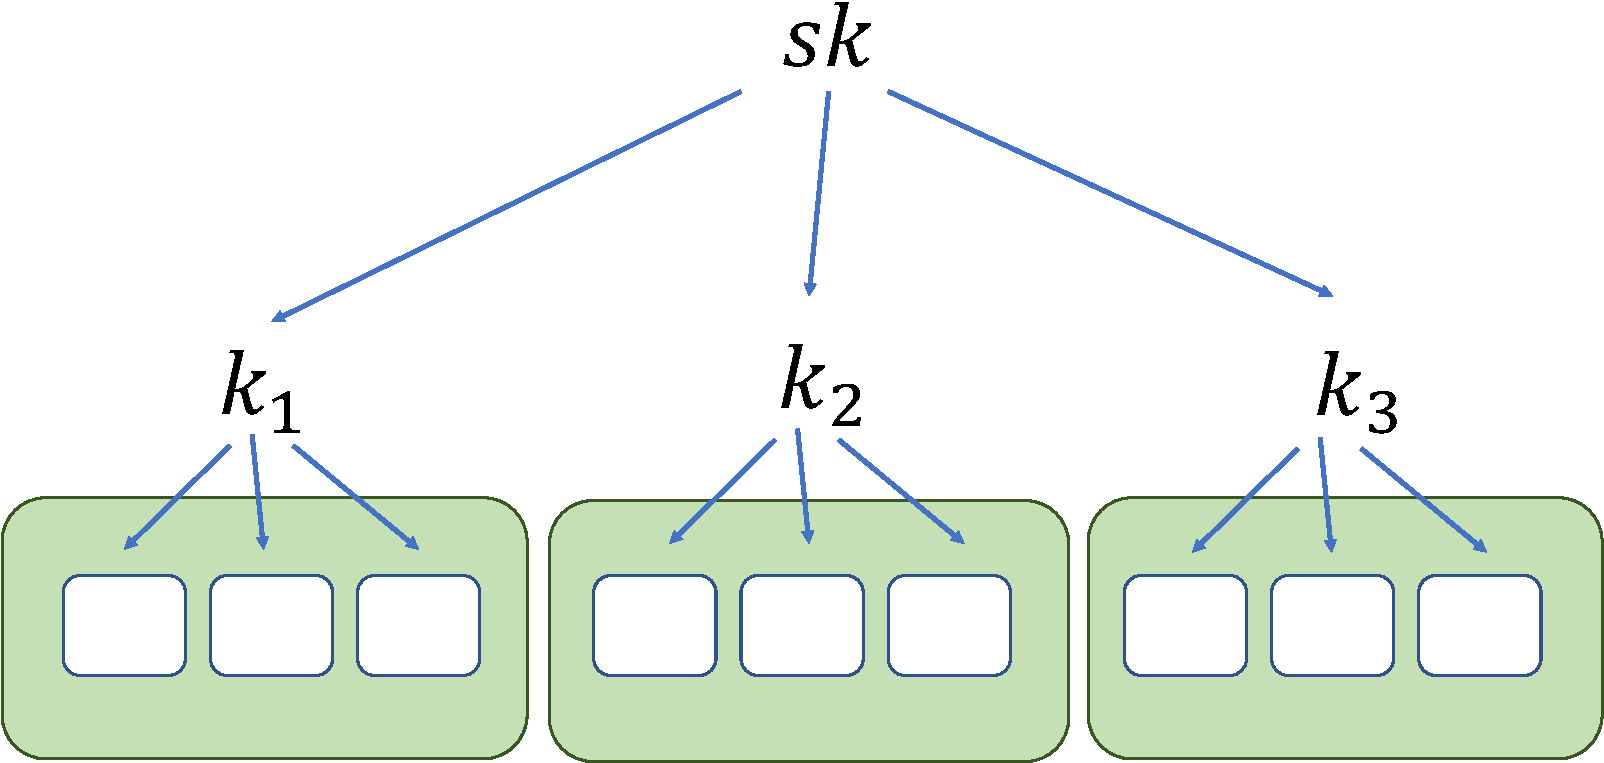
\includegraphics[width=0.6\linewidth]{figs/set-rep.pdf}
    \caption{Two-layer set representation\label{fig:set-rep}. The first layer key expands to $n^{1/4}$ sub-keys. Each sub-key controls a superblock and expands to $n^{1/4}$ offsets. Each offset in a chunk represents an index.}
\end{figure*}

%Here, $x[i:j]$ means the bit string from the $i$-th bit to the $(j-1)$-th bit of $x$'s binary representation.

Again, the high level idea behind the online query is similar: the client finds
a key $\sk$ such that $x\in \Set(\sk)$. The client wants to learn the parity of
$\Set(\sk_i)/\{x\}$. We now present in two-steps below how the two-layer set
representation helps us to reduce the online communication cost to
$\widetilde{O}_\lambda(n^{1/4})$ bits. 

\begin{itemize}
    \item \textit{Step 1: Learning the parities for all superblocks except the
    one containing $x$.}
    
    The client first expands $\sk$ to $n^{1/4}$ sub-keys,
    $k_0,\dots,k_{n^{1/4}-1}$. Now, the client replaces the $\superblock(x)$-th
    sub-key by a uniformly random sub-key $k'\getr\{0,1\}^\lambda$. This ensures
    that from the server's view, these $n^{1/4}$ sub-keys are random after the
    replacement. The client sends these $n^{1/4}$ sub-keys to the server. For
    each superblock $i$, the server will expand the $i$-th sub-key to $n^{1/4}$
    offsets and consider them as the offsets for the $n^{1/4}$ chunks in the
    superblock $i$. The server computes the parity for the $n^{1/4}$ indices
    corresponding to the offsets. Denote the parity as $\alpha_i$. The server
    returns $(\alpha_0,\dots,\alpha_{n^{1/4}-1})$ to the client. Then, except
    $\alpha_{\superblock(x)}$, all other $\alpha$ are the correct parities for
    their corresponding superblocks. The client can simply compute the xor-sum
    of those $n^{1/4}-1$ superblocks.

    \item \textit{Step 2: Learning the parity of all other indices in $x$'s
    superblock except $x$.} Now, the client expands $k_{\superblock(x)}$ to
    $n^{1/4}$ offsets, $\delta_0,\dots,\delta_{n^{1/4}-1}$. Notice that in the
    relative location of $x$'s chunk, the offset will be $x \mod \sqrt{n}$.
    Recall that the client already preprocessed polylogarithmic random
    replacement, i.e., index-value pairs in each chunk. Assume the first
    unconsumed replacement index in $x$'s chunk is $y$. The client simply
    replaces $x$'s offset to $y$'s offset and sends those $n^{1/4}$ offsets to
    the server. This ensures that from the server's view, these $n^{1/4}$
    offsets are random after the replacement. Upon receiving those offsets, the
    server does not know which superblock they correspond to. However, the
    server can just enumerate all $n^{1/4}$ possible cases: for
    $i\in\{0,\dots,n^{1/4}\}$, the server considers those $n^{1/4}$ offsets are
    the offsets of those items in the $n^{1/4}$ chunks of the $i$-th superblock,
    and computes the corresponding parity $\beta_i$. The server returns
    $(\beta_0,\dots,\beta_{n^{1/4}-1})$ to the client. The client knows that
    $\beta_{\superblock(x)}$ is the correct parity for $x$'s superblock, except
    that the index $x$ is replaced with $y$. After removing the influence of $y$
    (the client already knows $\DB[y]$), it knows the parity of those indices
    inside $x$'s superblock except $x$.

\end{itemize}

Finally, the client can learn the parity of $ \Set(\sk)/\{x\}$ by xoring the answers from step 1 and 2. Then the client can derive $\DB[x]$.
Notice that in this algorithm, the client sends $n^{1/4}$ sub-keys and $n^{1/4}$ offsets to the server, and the server returns $2n^{1/4}$ parities (bits) to the client. 
So the communication cost is $O_\lambda(n^{1/4})$.
Also, the server's computation time in both steps is simply $O_\lambda(\sqrt{n})$ without any further optimization.
We present the pseudocode for the single query algorithm in~\Cref{fig:single-query}.

\begin{figure}
    \centering
    \begin{subfigure}[b,labelformat=empty]{0.48\textwidth}
        \centering
        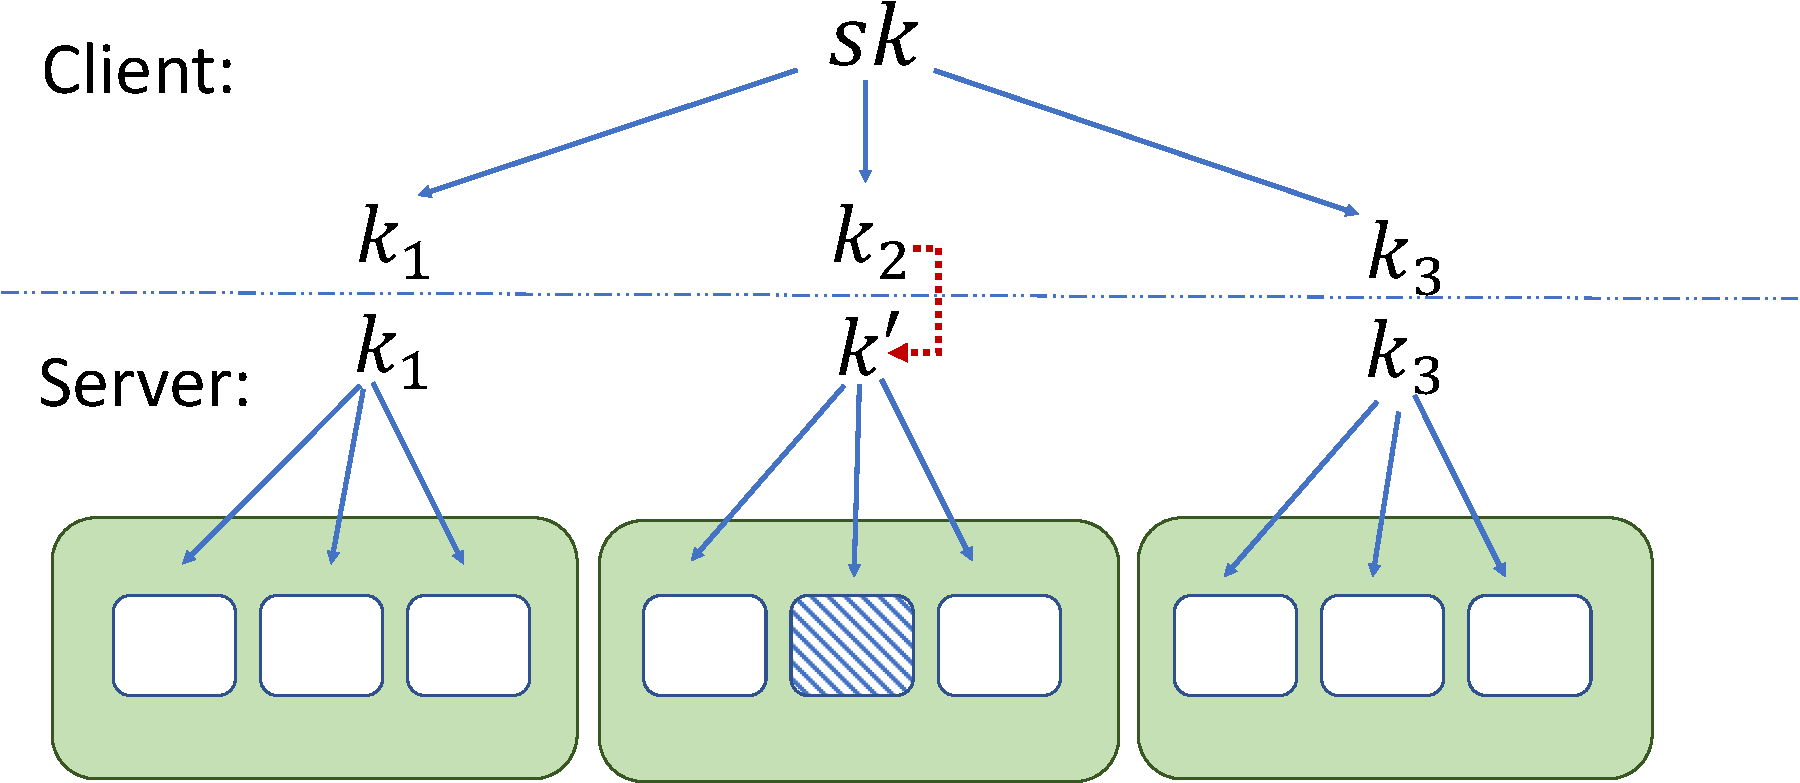
\includegraphics[width=\textwidth]{figs/step1.pdf}
        \caption*{Step 1: The client expands the main key to $n^{1/4}$ sub-keys and replaces the one that controls $x$'s superblock to a uniformly random one. The server returns $n^{1/4}$ parities for those $n^{1/4}$ superblocks.}
        % \label{fig:step1}
    \end{subfigure}
    \hfill
    \begin{subfigure}[b,labelformat=empty]{0.48\textwidth}
        \centering
        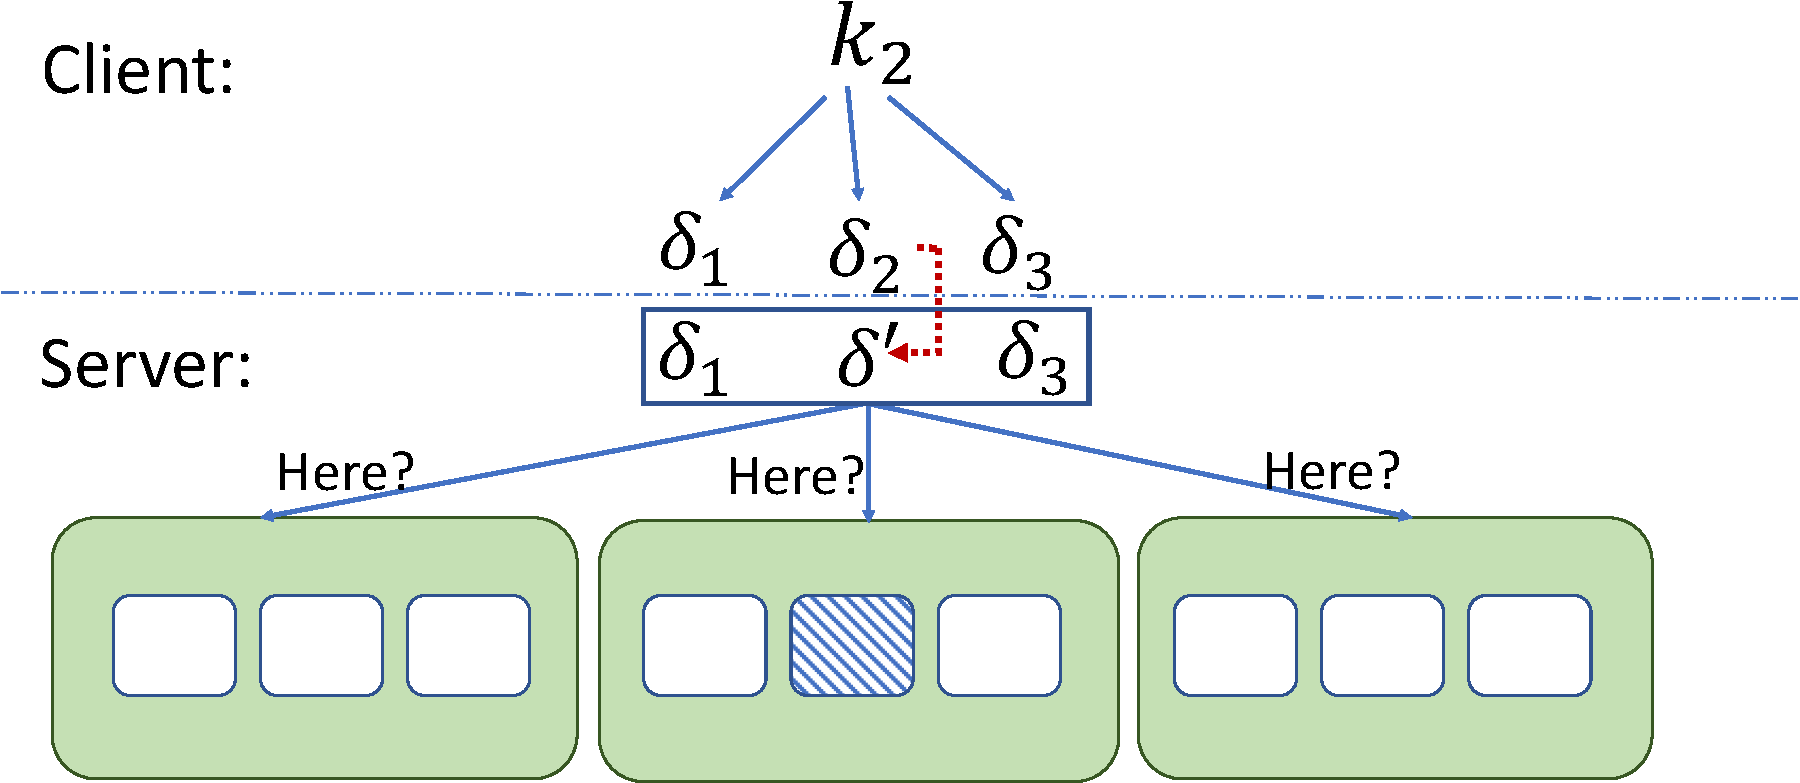
\includegraphics[width=\textwidth]{figs/step2.pdf}
        \caption*{Step 2: The client expands the sub-key to $n^{1/4}$ offsets and replaces the offset of $x$ to a random one. The server puts those offsets into every superblock. Returns $n^{1/4}$ corresponding parities. }
        % \label{fig:step2}
    \end{subfigure}
    \caption{Demonstration of the single-query algorithm assuming the query is in the middle chunk. The server does not know where the query is because the replacing operations are oblivious.}
    \label{fig:algo}
\end{figure}

%The main idea in our new construction is instead of sending over the offsets of $\sqrt{n}$ values, the client will send over $n^{1/4}$ ``sub-keys'' and $n^{1/4}$ offsets, thereby reducing the communication. The sub-keys will be $\lambda$ bits long and will correspond to a superblock. Further, a sub-key will be sufficient to compute all the offsets of a chunk in a superblock. 

%In order to read the value at index $x$, the client will compute the $n^{1/4}$ sub-keys for all the chunks, and compute all the offsets only for the chunks in same superblock as $x$ is in. The client then sends over {\bf 1)} all the sub-keys, except the one for the superblock of $x$, replacing it with a random sub-key {\bf 2)} all the offsets for the chunks in the superblock of $x$, except the offset for $\chunk(x)$, replacing it with the offset of a random element $r$ which is in $\chunk(x)$, such that $\DB[r]$ was stored during preprocessing.

%We need to specify how these sub-keys for the superblocks are computed given the $\PRF$ key. Here, we utilize the underlying structure of the $\PRF$ . We assume that the $\PRF:\bits^{\lambda}\times \bits^{\frac{\log n}{2}}\to \bits^{\frac{\log n}{2}}$ is constructed from two different $\PRF$'s $\PRF_1: \bits^{\lambda}\times \bits^{\frac{\log n}{4}}\to \bits^{\lambda},\PRF_2:\bits^{\lambda}\times \bits^{\frac{\log n}{4}}\to \bits^{\frac{\log n}{2}}$ as follows:
%\begin{align*}
%    \PRF(\sk,x)=\PRF_2(\PRF_1(\sk,x[0]),x[1])\;,
%\end{align*}
%where $x[0],x[1]$ denote the first $\frac{\log n}{4}$ and last $\frac{\log n}{4}$ bits of $x$ respectively. The GGM construction~\cite{GGM86} in particular can be viewed to be of this form.

%Given $\sk$, the sub-key for superblock $i$ is $k_i=\PRF_1(\sk,i)$ for $i\in \{0,1,\ldots,n^{1/4}-1\}$. Note that all the offsets for chunk $i$ can be computed using $k_i$. As specified above, the client sends over $n^{1/4}$ different sub-keys and $n^{1/4}$ different offsets to the server. Label the sub-keys received by the server as $k_0',k_1',\ldots,k_{n^{1/4}-1}'$ and label the offsets as $\delta_0',\delta_1',\ldots,\delta_{n^{1/4}-1}'$.

% \heading{Superblocks, sub-keys and the low bandwidth construction.} Let $x_0\in \bits^{\frac{\log n}{2}}$. Observe that, because of the property of $\PRF$, if the client provides the evaluation of $\PRF_1(\sk,x_0)$, the server can compute $\PRF(\sk,x_0\concat x_1)=\PRF_2(\PRF_1(\sk,x_0),x_1)$ for any $x_1\in \bits^{\frac{\log n}{2}}$. We use this observation to compress the online bandwidth.
% If the client wants to read the location $x$, and $\sk$ is a hint such that $x\in\Set(\sk)$, for all $y\in \{0,1,\ldots,n^{1/4}-1\}$, the client compute $\PRF_1(\sk,y)$. Let these values be $k_0,k_1,\ldots,k_{n^{1/4}-1}$ -- we refer to them as ``sub-keys''. 

% We introduce a new terminology: for every $x\in \{0,\ldots,{n}-1\}$ we say that $x$ is in the ``superblock" $j$ if $\lfloor x/n^{1/4}\rfloor = j$. Further, we say that the relative location of $\chunk(x)$ in superblock $j$ is $\chunk(x)-j\cdot n^{1/4}$. 

% We also refer to $k_j$ as the sub-key for that superblock. Let $b^*=\superblock(x)$ and $d^*$ be the relative location of $\chunk(x)$ in $\superblock(x)$, i.e. $d^*=\chunk(x)-\superblock(x)\cdot n^{1/4}$. Let $\delta_i=\PRF_2(k_{b^*},i)$ for $i\in \{0,1,\ldots,n^{1/4}-1\}$.
% Let $k'$ be a randomly sampled sub-key and let $r$ be a random value in $\{0,\ldots,n-1\}$ such that $\DB[r]$ such that $\chunk(r)=\chunk(x)$ had been read and stored by the client during the preprocessing. Let $\delta=r \text{ mod }\sqrt{n}$. The client sends over the following to the server:
% \begin{itemize}
%     \item the subkeys $k_0,\ldots,k_{n^{1/4}-1}$ \emph{except} $k_{b^*}$, replacing it with $k'$, 
%     \item the offsets $\delta_0,\ldots,\delta_{n^{1/4}-1}$ \emph{except} $\delta_{d^*}$, replacing it with $\delta'$.
% \end{itemize}

%For each $b\in \{0,\ldots,n^{1/4}-1\}$, the server computes the offsets for the $b$-th sub-key $k_b$, i.e. computes $\PRF_2(k_b',y)$ for each $y\in \{0,1,\ldots,n^{1/4}-1\}$. Assuming that this $b$-th sub-key is the sub-key for the $b$-th superblock (this assumption is correct except for the superblock $x$ is in), it computes the xor-sum of all the database entries indexed by the values in the superblock. Call this xor-sums $\alpha_b$. Next for $b\in  \{0,\ldots,n^{1/4}-1\}$, the server assumes that the offsets were of the $b$-th superblock and computes the xor-sum of the super-block accordingly (this assumption in contrast is \emph{only} correct for the superblock $x$ is in). Call the xor-sums $\beta_b$. The server sends over all the $\alpha_b$'s and $\beta_b$'s for $b\in  \{0,\ldots,n^{1/4}-1\}$ to the client.

\begin{figure}[p]
    
    \begin{minipage}{\textwidth}
        \begin{mdframed}
            \label{alg:one-query}
            \begin{center}
                {\bf Query Protocol for a Single Query $x$: $\SingleQuery(x,
                \sk, p_{\sk}, r, p_r)$.
                    %\andy{Is it not $O(\sqrt{n})$?}
                }
            \end{center}
            
            \parhead{Client's input:}
            %Suppose the client has the following inputs:
            \begin{itemize}
                \item A master PRF key $\sk$ assuming $x\in \Set(\sk)$;
                \item The parity of $\Set(\sk)$ is assumed to be $p_{\sk}$;
                \item A random index $r$ in $x$'s chunk such that the  $\DB[r]$
                is assumed to be $p_r$.
            \end{itemize}
            
            %\parhead{Suppose the client has a hint $$} When a query $x \in \{0,
            %1, \ldots, n-1\}$ arrives, \Client performs the following: 
            \begin{enumerate}[leftmargin=5mm,itemsep=1pt]
                \item 
                {\bf Step 1: (Client)}

                \begin{enumerate}[leftmargin=5mm,itemsep=1pt]
                        
                        \item Let $b^*={\sf superblock}(x)=\lfloor x/n^{3/4}
                        \rfloor, c^* = {\sf chunk}(x)=\lfloor x/n^{1/2}
                        \rfloor$. Let $d^*=\chunk(x)\mod n^{1/4}$ be the
                        relative chunk location of $x$ in the superblock. 
                        

                        \item Expand $\sk$ to $n^{1/4}$ sub-keys $k_{
                        0},\dots,k_{n^{1/4}-1}$ where $k_{b}=\PRF_1(\sk, b)$ for
                        all $b$.
                    
                        \item Expand the $b^*$-th sub-keys to $n^{1/4}$ offsets
                        $\delta_{0},\dots,\delta_{n^{1/4}-1}$ where
                        $\delta_{\ell}=\PRF_2(k_{b^*}, \ell)$.
                        
                        \item Sample a random sub-key $k'\getr\{0,1\}^\lambda$
                        and denote $\delta'=r\mod \sqrt{n}$.
                        \item Send the following tuples to the server:
                        \begin{align*}
                            (k_{0},\dots,k_{b^*-1}, k',k_{b^*+1},\dots,k_{n^{1/4}-1}) \\
                            (\delta_{0},\dots,\delta_{d^*-1},\delta' ,\delta_{d^*+1},\dots,\delta_{n^{1/4}-1})
                        \end{align*}
                    
                \end{enumerate}
                
                \newpage
                
                \item 
                {\bf Query Step 2: (Server)}
                
                Upon receving the tuples $(k'_0,\dots,k'_{n^{1/4}-1})$,
                $(\delta'_0,\dots,\delta'_{n^{1/4}-1})$: 
                \begin{enumerate}
                    \item For $b\in \{0,\dots,n^{1/4}-1\}$:
                    \begin{enumerate}
                        \item Expand $k'_b$ to $n^{1/4}$ offsets and consider
                        them being the corresponding index offsets in chunk $\{b
                        \cdot n^{1/4}, \ldots, (b + 1)\cdot n^{1/4} -1\}$.
                        Compute the xor-sum of the database values for those
                        indices as 
                        \[
                        \alpha_b=\xor_{c\in \{0,\dots,n^{1/4}-1\}} \DB[(c + bn^{1/4})\sqrt{n} + \PRF_2(k'_b, c)].
                        \]
                        \item Consider $(\delta'_0,\dots,\delta'_{j,n^{1/4}-1})$
                        as the corresponding index offsets in chunk $\{b \cdot
                        n^{1/4}, \ldots, (b + 1)\cdot n^{1/4} -1\}$. Compute the
                        xor-sum of the database values for those indices as 
                        \[
                        \beta_b=\xor_{c\in \{0,\dots,n^{1/4}-1\}} \DB[(c + bn^{1/4})\sqrt{n} + \delta_c].
                        \]
                    \end{enumerate}
                    
                    \item Return $(\alpha_0,\dots,\alpha_{n^{1/4}-1}),
                    (\beta_0,\dots,\beta_{n^{1/4}-1})$ to the client.
                \end{enumerate}
                
                
                \item 
               {\bf Step 3: (Client)}
               
               Upon receiving $(\alpha_0,\dots,\alpha_{n^{1/4}-1}),
               (\beta_0,\dots,\beta_{n^{1/4}-1})$:
                \begin{itemize}[leftmargin=5mm,itemsep=1pt]
                    \item 
                    The xor-sum of the items in $\Set(\sk)$ except those in the
                    superblock of $x$ is
                    $\alpha=\sum_{b\in\{0,\dots,n^{1/4}-1\},b\ne b^*}\alpha_b$.
                    
                    \item The xor-sum of the items in the superblock of $x$
                    except $x$ is $\beta=\beta_{b^*}\xor p_r$.
                    
                    \item Then, the value of $x$ is
                    $\DB[x]=p_\sk\xor\alpha\xor\beta$.
                \end{itemize}
            \end{enumerate}
        \end{mdframed}
    \end{minipage}
    \caption{Query Protocol for a single query that reduces communication to
    $O(n^{1/4})$. This is used as a sub-routine in the sublinear single server
    PIR scheme presented in Section~\labelcref{sec:nquarter}.}
    \label{fig:single-query}
\end{figure}



%Given all the $\alpha_b$'s the client can compute the xor sum of all the values
% indexed by $\Set(\sk)$, except for those in superblock of $x$. From the
% preprocessing the client knows the xor-sum of all the values indexed by
% $\Set(\sk)$ and thereby can compute the xor-sum of all the values indexed by
% the elements in the super-block of $x$. Further, the $\beta_b$'s along with
% the value of $\DB[r]$ for the $r$ client used specify can be used to compute
% $\DB[x]$ from the  xor-sum of all the values indexed by the elements in the
% super-block of $x$. Now, suppose $b^*=\superblock(x)$. Observe that $\alpha=
% \alpha_{b^*}\oplus \sum_{i=0}^{n^{1/4}-1}\alpha_i$ is the xor-sum of the
% database entries indexed by all the values at all the super blocks except
% super-block $b^*$. Further, $\beta=\beta_{b^*}\oplus p_r$ (where $p_r=\DB[r]$,
% the value of the database at $r$, which was stored by the client during
% preprocessing) is the xor-sum of all the entries of the database indexed by
% the values in the super-block $b^*$ except the value indexed by
% $\delta_{d^*}$. If $p_{\sk}$ was the parity of all the bits of the database
% indexed by $\sk$ (that the client stored during preprocessing), it follows
% that $\DB[x]=p_{\sk}\oplus\alpha\oplus \beta$. The client can compute this
% since it has stored $p_r,p_{\sk}$ during preprocessing and received rest of
% the values from the server.


\subsection{Supporting multiple queries in the online phase} 

Thus far, we have
given a new, low-communication protocol that handles only one query. We now want
to make $Q=\sqrt{n}/2$ queries with just one offline phase. For convenience, we
first make some assumptions about the queries without loss of generality, which
are also made in $\Piano$:
\begin{itemize}
    \item \textit{The client does not make repeated queries.} This can be ensured 
    by requiring the client to store a local cache of size $Q$ for caching the
    most recent $Q$ queries. If the client wants a repeated query, it can lookup
    in the cache and make a dummy query.
    
    \item \textit{The queries the client makes are on random indices.} This is a relatively
    strong assumption. However, we argue that it can be made without loss of
    generality and can be done by letting the client and the server agree on a
    pseudorandom permutation (PRP)~\cite{prp1,prp2} upfront and the server can
    permute the database according to the PRP. Another option is let the server
    build the database as a key-value storage and use a cuckoo hash
    table~\cite{cuckoo1,cuckoo2} directly based on a PRF to locate the queries.
    Notice that, in both implementations, the client can still make queries
    adaptively depending on the real query sequnce and the responses, which is
    sufficient for practical usage. Then, as long as the client makes the
    queries independent of the randomness of the PRP/PRF, those queries can be
    considered as uniformly random. This assumption is only needed for the
    correctness.
\end{itemize}

In order to support multiple queries, the key idea that had been used in
$\Piano$ was to ``refresh" the consumed hint by re-programming a fresh hint in a
way that does not change the distribution of the hints. Here, while our high
level goal will be the same, our strategy to do it would be significantly
different. The reason why the approach used in $\Piano$ does not translate here
is because of the following tension. Since in this new protocol we compress
bandwidth by making the client send only \emph{sub-keys} for the superblocks,
re-programming the hint while still having this compression would make
distribution of the client's future messages depend on the current query, which
violates privacy. Therefore, we seem to require newer ideas to avoid this issue.


Our main idea here is that when the client wants to read $x$, they find
\emph{all} the hints $\sk_i$ such that $x\in\Set(\sk_i)$. The client then runs
the single query protocol based on all of these hints\footnote{To ensure privacy, we
will have an probabilistic upper bound on how many queries are made. If the
client does not have that many hints, it pads some dummy queries.}. After these
hints have been consumed, the client needs to generate new hints so that the
distribution of local hints does not change. Here, for each consumed hint, the
client resamples a new key $\sk$ such that $x\in \Set(\sk)$ by rejection
sampling\footnote{The reason why the client cannot replace those hints with a
uniformly random one is that the occurrence of $x$ in the remaining tables are
less likely, and thus skewing the distribution.}. However, this could raise of
problem of ``broken hints'': the client does not know the parity for these newly
generated sets, and thus these new hints are marked as ``broken''. 

The key observation is this: as long as there is at least one non-broken hint
among the chosen hints, then the client can \emph{still} find the right
$\DB[x]$. And we will prove that except with negligible probability, at least
one of the hints for $x$ that the client chooses is not broken. Moreover, the
client only needs to consume the replacement index-value pairs for that single
query based on the one non-broken hint. For every other queries, the client does
not care about the response, so the client just replaces $x$'s offset with a
random offset. Notice that if the client shuffles the order of queries, the
query based on good hint and the queries based on the broken hints are
identically distributed from the server's view. Lastly, we argue that the client needs running time roughly $O(\sqrt{n})$ trials to rejection sample one hint in expectation. This follows since if we sample a random secret key
$\sk$, the probability that $\PRF(\sk,\chunk(x))=x-\chunk(x)\cdot \sqrt{n}$ is
$\Theta(1/\sqrt{n})$ assuming that the $\PRF$ was a random function. There are superlogarithmically many hints that need to be sampled.
This can be done in $\widetilde{O}(\sqrt{n})$ expected
time.

\begin{figure}[p]
    \begin{minipage}{\textwidth}
        \begin{mdframed}
            \label{alg:fullpolyl}
            \begin{center}
                {\bf Single-Server Scheme for $Q=\sqrt{n}/2$ Queries
                    \footnote{For clarity, we present the scheme supporting distinct and random queries. As mentioned before, these restrictions can be removed by applying PRP and local caching.}
                }
            \end{center}
            \parhead{Notation.}
            $\kappa$ denotes a {\it statistical} security parameter, $\lambda$
            denotes a computational security parameter. We use $\alpha(\kappa)$
            to denote an arbitrarily small super-constant function.

           \parhead{Offline preprocessing.} 
            \begin{itemize}[leftmargin=3mm,itemsep=1pt]
                \item 
                \Client samples $M_1=2\sqrt{n}\log \kappa \cdot \alpha(\kappa)$
                master PRF keys denoted $\psk_1, \dots, \psk_{M_1} \in \{0,
                1\}^\lambda$ for the primary table.
                %, where $M_1=\sqrt{n}\log \kappa \cdot \alpha(\kappa)$. , such
                %that $\alpha(n)=\omega(1)$. \elaine{TODO: fix params}
                Initialize the parities $p_1,\dots,p_{M_1}$ to zeros.
                
                %\elaine{TODO: notation inconsistent with earlier text}
                
                \item 
                \Client downloads the whole DB from the server in a streaming
                way: when the client has the $j$-th chunk
                $\DB[j\sqrt{n}:(j+1)\sqrt{n}]$:
                \begin{itemize}
                    \item {\it Update primary table}: for $i \in [M_1]$, let
                    $p_i \get p_i \oplus \DB[\Set(\psk_i)[j]]$.
                    \item {\it Store replacement entries}: sample and store
                    $M_2=3\log \kappa \cdot \alpha(\kappa)$ % \log \kappa\cdot
                    % \alpha(\kappa)$ 
                    tuples of the form $(r, \DB[r])$ where $r$ is a random index
                    from the $j$-th chunk.
                    %independent random indices from $[i\sqrt{n}:(i+1)\sqrt{n}]$
                    %with the associated database values.
                    \item Delete $\DB[j \sqrt{n}:(j +1)\sqrt{n}]$ from the local
                    storage.
                \end{itemize}
                
                \item At this moment, let $T := \{(\psk_i, p_i )\}_{i \in
                [M_1]}$ denote the client's {\it hint table}. Mark all the hints
                as ``good''.
            \end{itemize}
            
            
            
            
            \parhead{Online query for index $x \in \{0, 1, \ldots, n-1\}$.}
            %When a query $x \in \{0, 1, \ldots, n-1\}$ arrives, \Client
            %performs the following: 
            \begin{enumerate}[leftmargin=5mm,itemsep=1pt]
                \item 
                {\bf Query:}
                \begin{enumerate}[leftmargin=5mm,itemsep=1pt]
                    %\item Let %$i^*=\left\lfloor
                    %\frac{x}{\sqrt{n}}\right\rfloor$ be the index of $x$'s
                    %chunk.
                    \item 
                    \Client finds all the matched hints
                    $(\sk_1,p_1),\dots,(\sk_m,p_m)$ in the hint table  such that
                    $x\in \Set(\sk_j)$ for all $j\in[m]$.
                    
                    \item 
                    If there are less than $M_3=6(\ln \kappa \alpha(\kappa))^2$
                    hints, pad them with random broken hints. If there are more
                    than $M_3$ hints, sample $M_3$ hints from them. Randomly
                    shuffle the order of these hints\footnote{We add this random
                    shuffle to ensure that the order of the hints do not reveal
                    any information}.
                    %\item If there are more than $M_3$ matched hints, randomly
                    %choose $M_3$ hints among them. (see \Cref{eqn:setfromkey}
                    %for the definition of $\Set(\psk_j, x')$ where $x'$ is
                    %possibly $\bot$). 
                    
                    
                    % \item For the one of the randomly chosen good matched hint
                    % $(\sk_j, p_j)$\footnote{If there are no good matched hint,
                    % just mark the answer as 0.}:
                    % \begin{itemize}
                    %     \item \Client finds the first unconsumed replacement
                    %     entries $(r, \DB[r])$ from $x$'s chunk;
                    %     \item Execute $\SingleQuery(x, \sk_j, p_j, r, \DB[r])$
                    %     and mark the answer for the query.
                    % \end{itemize} 
                    
                    % \item Simultaneously, for other matched hints $(\sk_j,
                    % p_j)$: 
                    % \begin{itemize}
                    %     \item \Client executes $\SingleQuery(x, \sk_j, 0, r',
                    %     0)$ with a random index $r'$ from $x$'s chunk and
                    %     ignores the answer.
                    % \end{itemize}
                    \item For each hint, do the following:
            \begin{itemize}
                \item if the hint is marked good, find the first unconsumed replacement entry $(r, \DB[r])$ from $x$'s chunk;
                and execute $\SingleQuery(x, \sk_j, p_j,r,\DB[r])$ and store the answer for the query.
                \item Otherwise, execute $\SingleQuery(x, \sk_j, 0,0,r')$ with a random index $r'$ from $x$'s chunk  and ignore the answer.
            \end{itemize}
                
            \item Return the answer of any of the good hints. If none of the hints were good, just return $0$.
                    
                \end{enumerate}
                
                \item 
                {\bf Refresh:}
                \begin{itemize}
                    \item \Client replaces all the keys for the matched hints in
                    the hint table with $\sk'_1,\dots,\sk'_m$, such that for all
                    $j$, $\sk'_j$ is rejection-sampled conditioned on $x\in
                    \Set(\sk'_j)$. Also mark the parities as 0 and mark those
                    hints as ``broken''.
                \end{itemize}
                
            \end{enumerate}
        \end{mdframed}
    \end{minipage}
    \caption{Sublinear single server preprocessing PIR protocol introduced in
    Section ~\labelcref{sec:single-server}. The protocol uses $\SingleQuery$ defined
    in Fig.~\labelcref{fig:single-query} as a sub-routine.}
    \label{fig:single-server}
\end{figure}


\ignore{

To sum up the major changes in this construction compared to $\Piano$ are the
following.
\begin{itemize}
    \item Instead of sending over all the $n^{1/2}$ indices, the client sends
    $n^{1/4}$ sub-keys and $n^{1/4}$ offsets.
    %\item The preprocessing does not store backup hints for each chunk, instead
    %storing a super logarithmic number of random values $r$ and $\DB[r]$ for
    %each chunk.
    \item When querying $x$, online phase runs the protocol for single reads for
    all matched hints instead of just for the first one as in $\Piano$. At the
    end the client chooses the correct answer appropriately.
    \item When replacing a hint that was consumed for $x$, the client simply
    rejection samples a new hint, sets its parity to $0$ and marks it as broken.
\end{itemize}

}


\subsection{Putting everything together in the two-server setting}



So far we have been focused on the online phase.
We now introduce the implementation of the offline phase.

In the two-server setting, we assume there are two non-colluding servers and each one of them stores a replica of the database.
We call them the left server and the right server for convenience.

In fact, in the two-server setting, handling the offline phase is straightforwad.
After the client generates all $M_1=\widetilde{O}_\lambda(\sqrt{n})$ keys, 
the client will directly send the keys to the left server the left server expands those keys 
to sets.
Then, the left server returns the parities of those sets to the client.
Moreover, the client will sample polylogarithmic random indices in each chunk
and directly ask the left server about their values.
Then, the client only interacts with the right server during the online phase, just as the protocol we mentioned before.

We omit the pseudocode for the two-server version, which will be nearly the same as the single-server version presented later in~\Cref{fig:single-server}. 

\begin{theorem}
    Let $\lambda,\kappa\in \mathbb{N}$.
    Let $\alpha(\kappa)$ be any superconstant function. Assume $\PRF_1,\PRF_2$ is secure pseudorandom functions. Assume $n$ is bounded by $\poly(\lambda)$ and
    $\poly(\kappa)$. The two-server PIR scheme that supports $Q=\sqrt{n}/2$ queries is private, correct with probability
    $1-\negl(\lambda)-\negl(\kappa)$ where $\negl(.)$ is a negligible function. Further, it achieves the following performance
    bounds:
    
    
    \begin{itemize}
        \item $O(\lambda\sqrt{n}\log \kappa \alpha(\kappa))$ client storage and
        no additional server storage;
        \item \textbf{Offline Phase}:
        \begin{itemize}
            \item $O(\lambda n\log \kappa \alpha(\kappa))$ server time and
            $O(\lambda\sqrt{n}\log \kappa \alpha(\kappa))$ client time;
            \item \underline{$O(\lambda\sqrt{n}\log \kappa \alpha(\kappa))$
                communication}.
        \end{itemize}
        \item \textbf{Online Phase}:
        \begin{itemize}
            \item $O(\lambda\sqrt{n}\log \kappa \alpha(\kappa))$ expected client
            time and $O(\lambda\sqrt{n}(\log \kappa \alpha(\kappa))^2)$ server
            time per query; 
            \item $O(\lambda n^{1/4}(\log \kappa    \alpha(\kappa))^2)$
            communication per query.
        \end{itemize}
    \end{itemize}     
\end{theorem}

\subsection{Putting everything together in the single-server setting}

\label{sec:single-server}

In the single-server setting, we have to ensure that the preprocessing is server-oblivious to get privacy.
We can follow the same idea from $\Piano$~\cite{piano} such that the client downloads the whole database to do the preprocessing in a streaming fashion. 
    The client initializes all the hints and updates the hints along with the streaming.
    After the client completes the preprocessing, it interacts with the server during the online phase.
    To the server, the offline phase is oblivious, so this scheme is also private. 
    However, now the scheme has $O(n)$ offline communication cost, and the amortized offline communication cost per query will be $O(\sqrt{n})$, instead of $\widetilde{O}_\lambda(1)$ in the two-server setting.

We give a pseudocode description of the protocol for $Q=\sqrt{n}/2$ queries in the single-server setting in
Figures~\labelcref{fig:single-server}. 

%The corollary below follows from Theorem~\labelcref{thm:main1} and the above remarks.



\begin{theorem}
    \label{thm:main1} Let $\lambda,\kappa\in \mathbb{N}$.
    Let $\alpha(\kappa)$ be any superconstant function. Assume $\PRF_1,\PRF_2$ are secure pseudorandom functions. Assume $n$ is bounded by $\poly(\lambda)$ and
    $\poly(\kappa)$. The single-server scheme in~\Cref{fig:single-server} that supports
    $\sqrt{n}/2$ queries is private, correct with probability
    $1-\negl(\lambda)-\negl(\kappa)$ where $\negl(.)$ is a negligible function. Further, it achieves the following performance
    bounds:
    \begin{itemize}
        \item $O(\lambda\sqrt{n}\log \kappa \alpha(\kappa))$ client storage and
        no additional server storage;
        \item \textbf{Offline Phase}:
        \begin{itemize}
            \item $O(n)$ server time and $O(\lambda n\log \kappa \alpha(\kappa))$ client time
            ;
            \item \underline{$O(n)$ communication};
        \end{itemize}
        \item \textbf{Online Phase}:
        \begin{itemize}
            \item $O(\lambda\sqrt{n}\log \kappa \alpha(\kappa))$ expected client
            time and $O(\lambda\sqrt{n}(\log \kappa \alpha(\kappa))^2)$ server
            time per query; 
            \item $O(\lambda n^{1/4}(\log \kappa \alpha(\kappa))^2)$
            communication per query.
        \end{itemize}
    \end{itemize} 
\end{theorem}

\begin{proof}[Proof to~\Cref{thm:main1} and~\Cref{thm:main2}]
    
    We defer the privacy and the correctness proof to~\Cref{sec:proof}.

    The client only stores $M_1=2\sqrt{n}\log \kappa\alpha(\kappa)$
    $\lambda$-bit keys and store in total $\sqrt{n}\cdot M_2=3\sqrt{n}\log
    \kappa\alpha(\kappa)$ index-value pairs. So the storage is
    $O(\lambda\sqrt{n}\log \kappa \alpha(\kappa))$.
    
    The offline performance bounds follow straightforward by the algorithm descriptions.
    
    For the online phase, the client first enumerates all $M_1$ hints to find
    $x$, which takes $O(\lambda\sqrt{n}\log \kappa\alpha(\kappa))$ time. For all
    the $M_3=\Theta((\log \kappa \alpha(\kappa))^2)$ found hints, the
    $\SingleQuery$ algorithm takes $O(\lambda n^{1/4})$ client computation and
    $O(\lambda \sqrt{n})$ server computation, while the communication cost is $O(\lambda
    n^{1/4})$. During the refresh phase, we consider the expected computation time: each hint in the table will have $1/\sqrt{n}$ probability to be resampled and each resample takes $O(\lambda\sqrt{n})$ expected time to finish. 
    So the total expected time for the online phase is $O(\lambda\sqrt{n}\log \kappa
    \alpha(\kappa))$  per query. The online server time is
    $O(\lambda\sqrt{n}(\log \kappa \alpha(\kappa))^2)$ per query. The online
    communication per query is $O(\lambda n^{1/4}(\log \kappa
    \alpha(\kappa))^2)$.
\end{proof}



\paragraph{Supporting unbounded number of queries.}
The aforementioned scheme supports $Q=\sqrt{n}/2$ queries. 
We need a scheme that supports unbounded number of queries. 
We discuss different options below.

\begin{itemize}
    \item \textit{Repeating the $Q$-query scheme}. 
    The straightforward way is that once the client finishes a window of $Q$ queries, the client and the server(s) rerun the preprocessing phase again, using fresh randomness. 
    The drawback is that the client has to wait a long time before starting the next window.
    
    \item \textit{Pipelining the proprocessing and online phase}.
    It follows the same idea as in $\Piano$~\cite{piano}.
    The scheme first runs a preprocessing phase for the first $Q$ queries. 
    Then, during the online phase, the client interacts with the preprocessing server and gradually finishes the preprocessing for the next $Q$ queries. 
    Essentially, the client and the server can split the work (including computation and communication) of the preprocessing into $Q$ pieces.
    Whenever the client finish a query, the client and the preprocessing server will finish the next piece of work about preprocessing.
    Once the client finishes the $Q$ queries, it can immediately starts the next window of $Q$ queries because the preprocessing for the next window is done. 
    The main advantage is that the client never waits long time after the first preprocessing phase.
    The downside is: 1) in the two server setting, it requires the preprocessing server to be always online; 2) in the single-server setting, the online communication will be dominated by the preprocessing parts and become $O(\sqrt{n})$, instead of $\widetilde{O}_\lambda(n^{1/4})$.
\end{itemize} 






%Suppose the client has the master PRF key $\sk$ such that 



\subsection{Removing multiple $\SingleQuery$ executions via online resampling}

%\label{sec:optimized}


In the schemes mentioned in~\Cref{sec:main-scheme}, each online query will need
$6(\ln \kappa \alpha(\kappa))^2$ calls to the subroutine, $\SingleQuery$, and
each routine needs $O(\lambda n^{1/4})$ communication cost. In this section, we
introduce a slightly more involved scheme that requires \textbf{only one} call
to the $\SingleQuery$ subroutine per query.

\paragraph{Why previous schemes do not worry about broken hints.} First, we need
to understand why in the previous schemes like $\Piano$~\cite{piano}, the client
does not have to worry about broken hints. To ensure all hints are useful, the
client will prepare polylogarithmic backup hints for each of the $\sqrt{n}$
chunks. The backup hints for the $i$-th chunk will record the parity of the set
and also the value of the item in the $i$-th chunk. After querying for $x$, the
client will replace the consumed hint with a backup hint from $x$'s chunk and
replace that $i$-th element of the hint to the current query $x$, which
maintains the distribution of the hint table. Since the values for the original
$i$-th element and $x$ are known to the client, the correct parity for the
edited hint can be derived by the client locally and the new hint will always be
good. Then, the client only needs to find the first hint that contains $x$,
instead of finding all matched hints and making multiple queries based on those
hints, hoping that one of them will be good.~\footnote{A natural question is why
the client cannot simply pick the first good hint. Observe that it would be
equivalent to deleting a consumed hint from the table because a broken hint will
never be used again. Then, it would skew the distribution of the hint table
because the remaining hints are  less likely to contain the past queries, which
leads to privacy leakage.}

Notice that the hint replacement operation in $\Piano$ is done \textbf{lazily
and obliviously}: the client only stores the PRF key and the replacement
location, and only replaces the element when expanding the PRF key to a full set
of size $\sqrt{n}$ during the online query. The replacement operation is
oblivious to the server because the client will send all $\sqrt{n}$ indices to
the server, and swapping out one index with another one locally leaves no trace
of which index being replaced!

Unfortunately, this is not straightforward if we send the whole set to the
server and optimize the communication cost to $\widetilde{O}(n^{1/4})$.
%Remember that the client will send $n^{1/4}$ sub-keys to the server.
One way to achieve that is by ```programming'': when we promote a backup hint to
the primary hint table after a query, we somehow \textbf{program} the PRF
$\sk'$, so that the result of evaluating $\sk'$ on $x$'s chunk index is enforced
to be $x$'s offset. Also, the programmed PRF key should not leak the information
about which location has been programmed. Indeed, this is exactly the idea in
two previous single-server PIR schemes~\cite{pir-ec23,lazza-pir}, where they
utilized a heavy cryptographic construction called privately programmable
pseudorandom function (PPPRF) to achieve such programming operation. However,
this primitive is only known under strong cryptographic assumptions like LWE. 

\paragraph{Our solution: rejection sampling.} 
We observe that all we need to do is just to ``maintain'' the right distribution
of the hint table and the keys sent to the server. Then, we can rejection-sample
the PRF keys according to the right distribution and avoid the burden of doing
difficulty of doing private programming on the key level.

Maintaining the distribution for the local hint table is relatively simple. For
the local hint table, what we actually care about is the distribution of the
actual sets, regardless how we represent them. Assume that the client already
queries for $y$ and knows $\DB[y]$. Now the client consumes a hint that contains
$y$, and replaces it with a hint from those backup hints prepared for
$\chunk(y)$. Suppose the key for the backup hint is $\sk$. $\sk$ may not contain
$y$, but we can mark $y$ alongside the key, such that whenever we use the hint
later, we will manually enforce $y$ into the set.
\begin{figure}[p]
    
    \begin{minipage}{\textwidth}
        \begin{mdframed}
            \label{alg:optimized:full}
            \begin{center}
                {\bf Optimized Single-Server Scheme for $Q=\sqrt{n}/2$ Queries
                    \footnote{For clarity, we present the scheme supporting distinct and random queries.}
                }
            \end{center}
            \parhead{Notation.}
            $\kappa$ denotes a {\it statistical} security parameter, $\lambda$
            denotes a computational security parameter. We use $\alpha(\kappa)$
            to denote an arbitrarily small super-constant function.
            
            
            \parhead{Offline preprocessing.} 
            %\ \\[-6pt]
            \begin{itemize}[leftmargin=3mm,itemsep=1pt]
                \item In addition to the previous algorithm:
                \begin{itemize}
                    \item \Client samples $M_2=3\log \kappa \alpha(\kappa)$
                    backup keys $\sk_{i,1},\dots,\sk_{i,M_2}$ for chunk $i$;
                    \item For each backup hint, \Client stores $\sk_{i, j}$ and
                    the following information:
                    \begin{itemize}
                        \item The parity for the whole set: $p_{i,j}=\xor_{x\in
                        \Set(\sk_{i,j})} \DB[x]$;
                        \item The parity for those items within the superblock
                        that contains the $i$-th chunk: $b_{i,j}=\xor_{x\in
                        \Set(\sk_{i,j})} \I\left[\superblock(x) = \left\lfloor
                        \frac{i}{n^{1/4}} \right\rfloor
                        \right]\DB[x]$\footnote{$\I[A]$ is 1 when $A$ is true
                        and 0 otherwise.}
                       
                        \item The DB-value of the $i$-th item:
                        $\DB[\Set(\sk_{i,j})[i]]$. 
                    \end{itemize}
                \end{itemize}  
                
                             
                %\item At this moment, let $T := \{(\psk_i, p_i )\}_{i \in
                %[M_1]}$ denote the client's {\it hint table}. Mark all the
                %hints as ``good''.
            \end{itemize}
            
            
            
            
            \parhead{Online query for index $x \in \{0, 1, \ldots, n-1\}$.}
            %When a query $x \in \{0, 1, \ldots, n-1\}$ arrives, \Client
            %performs the following: 
            \begin{enumerate}[leftmargin=5mm,itemsep=1pt]
                \item 
                {\bf Query:}
                \begin{enumerate}[leftmargin=5mm,itemsep=1pt]
                    %\item Let %$i^*=\left\lfloor
                    %\frac{x}{\sqrt{n}}\right\rfloor$ be the index of $x$'s
                    %chunk.
                    \item 
                    \Client finds {the first} matched hint $(\sk_i, p_i)$
                    such that $x\in \Set(\sk_i)$ and the hint does not have a
                    positive constraint $y$ that $\chunk(y)=\chunk(x)$.

                        \item If there is no positive constraint on this hint:
                        execute $\SingleQuery$ as before (consuming a
                        replacement entry from $\chunk(x)$).
                        \item  If there is a positive constraint $+y$ on this
                        hint: 
                        \begin{enumerate}
                            \item If $\superblock(y)=\superblock(x)$, execute
                            $\SingleQuery$ as before, except:
                            \begin{itemize}
                                \item After expanding the sub-key to $n^{1/4}$
                                offsets, replace the $(\chunk(y) \mod
                                n^{1/4})$-th offset with $y$'s offset; 
                                \item If the return value is $v$, mark the
                                answer as $v\xor\DB[y]\xor
                                \DB[\Set(\sk_i)[\chunk(y)]]$. 
                            \end{itemize}

                           \item If $\superblock(y) \ne \superblock(x)$, execute
                           $\SingleQuery$ as before, except:
                           \begin{itemize}
                               \item After expanding $\sk_i$ to $n^{1/4}$
                               sub-keys, replace the $\superblock(y)$-th key
                               with a rejection-sampled key $k'$. The rejection
                               sampling key $k'$ should satisfy all constraints
                               related to the matched hint $(+y,
                               -z_1,\dots,-z_t)$ if $k'$ controls
                               $\superblock(y)$ (as specified in
                               Section~\labelcref{sec:optimized}).
                               
                               \item If the return value is $v$, mark the answer
                               as $v\xor\beta_{\superblock(y)}\xor b$, where
                               $\beta_{\superblock(y)}$ is the corresponding
                               parity of superblock controled by the
                               rejection-sampled sub-key and $b$ is the original
                               parity for that superblock, known by
                               preprocessing. 
                           \end{itemize}
                           
                            
                        \end{enumerate}
                                    
                \end{enumerate}
                
                \item 
                {\bf Refresh:}
                \begin{itemize}
                    \item \Client adds the constraint $-x$ for the first $i-1$
                    entries.
                    \item \Client replaces the matched hint with an unconsumed
                    hint from the $\chunk(x)$'s backup hint group. Clean all
                    other constraints and only mark $+x$ for the $i$-th entry.
                \end{itemize}
                
            \end{enumerate}
        \end{mdframed}
    \end{minipage}
    \caption{The optimized sublinear single server preprocessing PIR protocol
    introduced in Section ~\labelcref{sec:optimized}. The protocol uses
    $\SingleQuery$ defined in Fig.~\labelcref{fig:single-query} as a
    sub-routine.}
    \label{fig:optimized:single-server}
\end{figure}


The more tricky case is how we handle the keys that the client send to the
server. Suppose client is now querying for $x$, and it finds the first hint that
contains $x$. Also, it notices that the hint is marked with $y$. Recall that in
the $\SingleQuery$ algorithm the client will expand the master key into
$n^{1/4}$ keys and expand the keys corresponding to the superblock of $x$ to
$n^{1/4}$ offsets. Now there are two cases:
\begin{enumerate}
    \item \textit{$x$ and $y$ are in the same superblock.} This is a relatively
    simple case. We will always replace the sub-key corresponding to the
    superblock of $x$ (the same as $y$) with a uniformly random sub-key. Then,
    when we expand the original sub-key to $n^{1/4}$ offsets, we need to replace
    $x$'s offset with a random one, and also manually set the offset
    corresponding to $y$'s chunk to $y$'s offset, reflecting that we enforce $y$
    to be included in this hint. No rejection sampling is required in this case.
    
    For the answer, since we are just replacing the element in $y$'s chunk to
    $y$, the influence of such change should be removed. We can require the
    client to store the database value for the $i$-th element for all the backup
    hints dedicated for the $i$-th chunk. Then, if this promoted hint $\sk$ is
    used, we can correct the answer by xoring the influnce value,
    $\DB[\Set(\sk)[\chunk(y)]]\xor\DB[y]$.
    
    \item \textit{$x$ and $y$ are in the different superblocks.} This is the
    more involved case. We will again replace the sub-keys corresponding to
    $x$'s superblock with a uniformly random sub-key and replace the offsets in
    $x$'s chunk with a random one. However, we need to ensure that the key
    corresponding to $y$'s superblock will expand to the correct offset for
    $y$'s chunk, to ensure that $y$ is included. Now, we will rejection-sample a
    sub-key $k$ for $y$'s superblock, such that it expands to the correct offset
    of $y$. This is what we refer to as a \textbf{positive} constraint, and we
    write this constraint as $+y$.
    %We identify that this is \textbf{not enough} to ensure privacy.
    Additionally, to maintain the right distribution, there are also
    \textbf{negative} sampling constraints. Observe that if the $i$-th hint
    entry is the first one to contains $x$, it means that from the client's
    perspective, the first $i-1$ entries does not contain $x$. Suppose between
    the query $y$ and query $x$, there are some other queries. After making
    those queries, we also know that the current hint entry does not contain
    some queries $z_1,\dots,z_t$ in $y$'s superblock. We write down the negative
    constraints as $-z_1,\dots,-z_t$. Then, when we do the rejection sampling
    for the sub-key for $y$'s superblock, we will consider all the constraints:
    $+y, -z_1,\dots,-z_t$, until we find a sub-key $k$ that satisfies all the
    constraints. This ensures that the sub-key for $y$'s superblock has the
    right distribution.
    
    We also need to argue that the rejection-sampling is efficient. The positive
    constraint is satisfied with probability $1/\sqrt{n}$. Conditioned on the
    positive constraint being satisfied, for each negative constraint, it is
    satisfied with probability at least $1-1/\sqrt{n}$. We only aim to support
    $Q=\sqrt{n}/2$ queries within one window, so there are no more than
    $\sqrt{n}/2$ negative constraints. By union bound, satisfying all negative
    constraints happens with probability at least $1/2$. Therefore, we conclude
    that a freshly sampled sub-key satisfies all the constraints with
    probability at least $1/2\sqrt{n}$, and the expected sample time is
    $O(\sqrt{n})$. 
    
    A noticable detail is that when we draw a new fresh key,
    we first check the positive constraint. Only when the positive constraint is
    satisfied, we check the negative constraints. The positive constraint is
    satisfied with probability $1/\sqrt{n}$ but only takes $O(1)$ time to check.
    Conditioned on the positive constraint being satisfied, the negative
    constraints take $O(\sqrt{n})$ to check but are satisfied with probability
    at least $1/2$. So even including the constraint checking time, the expected
    sampling time is still $O(\sqrt{n})$.
    
    For the answer, since we are essentially replacing the original superblock
    to a rejection-sampled one. To remove the influence of this step, we can
    require the client to store the parity for the corresponding superblock
    controlling the $i$-th chunk for all the backup hints dedicated for the
    $i$-th chunk. Then, if this promoted hint $\sk$ is used, we can correct the
    answer by xor-ing the parity for the original superblock (known by preprocessing) and the parity for the
    rejection-sampled superblock (known from the online
    query).%$\DB[\Set(\sk)[\chunk(y)]]\xor\DB[y]$.    
    
\end{enumerate}


We provide the pseudocode of this construction in
Figure~\labelcref{fig:optimized:single-server}.

\begin{theorem}
    \label{thm:main2}
    Let $\alpha(\kappa)$ be any superconstant function. Assume $n$ is bounded by
    $\poly(\lambda)$ and $\poly(\kappa)$. The PIR scheme
    in~\Cref{fig:optimized:single-server} that supports $\sqrt{n}/2$ queries is
    private, correct with probability $1-\negl(\lambda)-\negl(\kappa)$ and
    achieves the following performance bounds (\underline{the optimized parts
    are underlined}):
    \begin{itemize}
        \item $O(\lambda\sqrt{n}\log \kappa \alpha(\kappa))$ client storage and
        no additional server storage;
        \item \textbf{Offline Phase}:
        \begin{itemize}
            \item $O(\lambda n\log \kappa \alpha(\kappa))$ client time and
            $O(n)$ server time;
            \item $O(n)$ communication;
        \end{itemize}
        \item \textbf{Online Phase}:
        \begin{itemize}
            \item \underline{$O(\lambda\sqrt{n})$ expected client time} and
            \underline{$O(\lambda\sqrt{n})$ server time} per query; 
            \item \underline{$O(\lambda n^{1/4})$ communication} per query.
        \end{itemize}
    \end{itemize} 
\end{theorem}

\begin{proof}
    We defer the privacy and the correctness proof to~\Cref{sec:deferred}.
    
    The additional storage for the client will be those $M_2$ backup hints per
    chunk, which results in total of $O(\lambda\sqrt{n}\log \kappa
    \alpha(\kappa))$ space. Notice that the client does not directly store the
    negative constraints, otherwise the storage will be blown up. The client can
    directly store the history of those matched hint entry index (which takes
    $O(\sqrt{n}\log n)$ space) and also the generation time label of each hint.
    Whenever the client finds the first matched hint, say entry $i$, it finds
    all the previous queries that are older than the current hint's generation
    time and whose matched hint entry indices are larger than $i$. Those history
    queries will be the negative constraints. By doing this, maintaining all the
    constraints only takes $O(\sqrt{n}\log n)$ space.
    
    %The client only stores $M_1=\sqrt{n}\log \kappa\alpha(\kappa)$
    %$\lambda$-bit keys and store in total $\sqrt{n}\cdot M_2=\sqrt{n}\log
    %\kappa\alpha(\kappa)$ index-value pairs. So the storage is
    %$O(\lambda\sqrt{n}\log \kappa \alpha(\kappa))$.
    
    The offline performance bounds are obvious by the algorithm description.
    
    For the online phase, the client first finds the first hint that contains
    $x$. Each hint contain $x$ with probability $1/\sqrt{n}$, so the expected
    time is $O(\lambda\sqrt{n})$. The $\SingleQuery$ algorithm takes $O(\lambda
    n^{1/4})$ client computation and $O(\lambda \sqrt{n})$ server computation,
    while consuming $O(\lambda n^{1/4})$ communication cost. The refresh phase
    takes only $O(1)$ time (if the client maintains the negative constraint
    using the technique mentioned above). So the online expected client time is
    $O(\lambda\sqrt{n})$ per query. The online server time is
    $O(\lambda\sqrt{n})$ per query. The online communication per query is
    $O(\lambda n^{1/4})$ per query.
\end{proof}


%\fi
% 
% \section{Correctness and Privacy Proofs}

We present the formal correctness and privacy proofs for the single-server scheme described in~\Cref{sec:main}.
We omit the proofs for the two-server scheme, which will be nearly the same as the proofs presented in this section.

\label{sec:proof}

\begin{theorem}[Privacy]
    The PIR scheme in \Cref{fig:single-server} is a secure single-server preprocessing PIR scheme assuming $\PRF$ is a secure pseudorandom function.
    \label{thm:privacy}
\end{theorem}

\begin{proof}
    We first need to prove the lemma that the \SingleQuery~algorithm is indeed private when the input $\sk$ is sampled according to the right distribution.
    
    \begin{lemma}
        \label{lem:privacy-single}
        Given any $x\in\{0,\dots,n-1\}$, let $b^*={\sf superblock}(x)=\lfloor x/n^{1/4} \rfloor, c^* = {\sf chunk}(x)=\lfloor x/n^{1/2} \rfloor$. Let $d^*=\left\lfloor\chunk(x)-\superblock(x)\cdot {n^{1/4}}\right\rfloor$ be the relative chunk location of $x$ in the superblock. 
        The following two experiments are indistinguishable:
        
        \begin{itemize}
            \item ${\sf RealSingleQuery:}$ 
            \begin{itemize}
                \item Sample a PRF key $\sk\getr\{0,1\}^\lambda$ conditioned on $x\in\Set(\sk)$;
                \item Let $k_{b^*}=\PRF_1(\sk, b^*)$.
                \item Sample a random PRF sub-key $k'\getr\{0,1\}^\lambda$;
                \item Sample a random offset $r'\getr\{0,\dots,\sqrt{n}-1\}$;
                \item The adversary receives
                \begin{align*}
                    (\PRF_1(\sk, 0),\dots,\PRF_1(\sk, b^*-1),k', \PRF_1(\sk, b^*+1),\dots,\PRF_1(\sk, n^{1/4}-1)),\\
                    (\PRF_2(k, 0),\dots,\PRF_1(k, d^*-1),r', \PRF_2(k, d^*+1),\dots,\PRF_2(k, n^{1/4}-1)).
                \end{align*}
            \end{itemize}
            
            \item ${\sf IdealSingleQuery:}$
            \begin{itemize}
                \item Independently sample $k_0,\dots,k_{n^{1/4}-1}\getr\{0,1\}^\lambda$;
                \item Independently sample $r_0,\dots,r_{n^{1/4}-1}\getr\{0,\dots,\sqrt{n}-1\}$.
                \item The adversary receives $(k_0,\dots,k_{n^{1/4}-1}),
                (r_0,\dots,r_{n^{1/4}-1})$.
            \end{itemize}
            
        \end{itemize}
        
        
    \end{lemma}
    
    \begin{proof}
        Observe that ${\sf RealSingleQuery}$ is just a re-write of the real experiment of $\SingleQuery$ that gets rid of the irrelevant parts.
        
        We can build a hybrid as the following ways: in this hybrid, instead of sampling a master key $\sk$, the experiment sample $n^{1/4}$ PRF sub-keys randomly $k_0,\dots,k_{n^{1/4}-1}$, conditioned on $\PRF_2(k_{b^*}, d^*)=\offset(x)$, i.e., it will correctly expand to the offsets containing $x$. It sends $(k_0,\dots,k_{b^*}-1,k',k_{b^*}+1,\dots,k_{n^{1/4}-1})$ as the first tuple to the adversary. Everything else is the same as ${\sf RealSingleQuery}$. Since the rejection-sampling condition is the same, due to the pseudorandomness of $\PRF_1$, this hybrid is computationally indistinguishable from ${\sf RealSingleQuery}$. 
        
        We build another hybrid such that it is the same as the first hybrid, except that it samples $r_0,\dots,r_{n^{1/4}-1}$ uniformly random conditioned on $r_{d^*}=\offset(x)$ and sends $(r_0,\dots,r_{d^*}-1,r',r_{d^*}+1,\dots,r_{n^{1/4}-1})$ to the adversary.
        Due to the pseudorandomness of  $\PRF_2$, this hybrid is computationally indistinguishable from the previous one.
        
        Now we see that the second hybrid has the same distribution as ${\sf IdealSingleQuery}$ due to the independence during the sampling procedure.
        So we prove the statement.
    \end{proof}
    
    \begin{remark}
        \label{lem:privacy-random}
        The previous lemma still holds if one just samples a uniform random PRF key $\sk$ (instead of conditioning on $x\in\Set(\sk)$).
    \end{remark}
    
    Now we are ready to prove the multi-query PIR scheme is private. We first define a hybrid ${\sf Real^*}$:
    
    
    \begin{itemize}
        \item \textit{Offline.} $\adv$ receives the streaming signal. The client samples $\sk_1,\dots,\sk_{M_1}\getr\{0,1\}^\lambda$.  
        \item \textit{Online.} For each round $t$, $\adv$ chooses a query $x_t$:
        \begin{itemize}
            \item The client finds all the matched keys $\sk_j$ in the hint table, that is, $x\in\Set(\sk_j)$. If there are less than $M_3$ of them, pad them with random keys. If there are more than $M_3$, down-sample to $M_3$ keys.

            \item For all those $M_3$ keys, first sample $r$ as a random index from $x$'s chunk. Then, the client and the server executes $\SingleQuery(x, \sk_j, 0, r, 0)$.
            
            \item For all matched keys in the hint table, replace them with a rejection-sampled random key $sk'_j$ conditioned on $x\in\Set(\sk'_j)$.
        \end{itemize}
        
    \end{itemize}
    
    Notice that this hybrid is identically distributed as the actual experiment -- we don't care about good or broken hints because we don't care about correctness here. All events related to good or broken hints is not observable by the server. We now define the ideal experiment  ${\sf Ideal}$:
    
    
    \begin{itemize}
    \item \textit{Offline.} $\adv$ receives the streaming signal. 
    \item \textit{Online.} For each round $t$, $\adv$ chooses a query $x_t$:
    \begin{itemize}
        \item The client repeats the following procedure for $M_3$ times with independent randomness:
        \begin{itemize}
                \item Independently sample $k_0,\dots,k_{n^{1/4}-1}\getr\{0,1\}^\lambda$;
                \item Independently sample $r_0,\dots,r_{n^{1/4}-1}\getr\{0,\dots,\sqrt{n}-1\}$.
                \item Send $(k_0,\dots,k_{n^{1/4}-1}),
                (r_0,\dots,r_{n^{1/4}-1})$ to the server.
        \end{itemize}
     \end{itemize}
    
    \end{itemize}    
   
    The following lemma shows that ${\sf Ideal}$ and ${\sf Real^*}$ are computationally indistinguishable.
    
    \begin{lemma}
        \label{lem:inductive-proof}
        In ${\sf Real^*}$, for each query $x_t$, even conditioned on $\adv$'s view over the first $t-1$ queries, 
        
        \begin{itemize}
            \item The messages $\adv$ receives are identically distributed to those in $\Ideal$ in this round;
            \item At the end of the $t$-th query, the client's local hint table  is identically distributed as sampling $M_1$ random PRF keys.
        \end{itemize}
    \end{lemma}
    
    \begin{proof}
        \textbf{Base Case}. At the end of the offline phase, the local hint table is indeed identically distributed as sampling $M_1$ random PRF keys.
        
        \textbf{Inductive Case}. Suppose at the end of $t-1$ round, the client's local hint table is identically distributed as sampling $M_1$ random PRF keys even conditioned on $\adv$'s view in the first $t-1$ steps.
        
        Consider the following experiment $\Expt$:
        \begin{itemize}
            \item The client first samples $m$ according to the distribution of the number of matched hints if the hint table is indeed freshly-random;
            \item The client sample $m$ PRF keys $\sk_1,\dots,\sk_m$ conditioned on $x\in \Set(\sk_j)$;
            \item If there are less than $M_3$ keys, the client pads with random keys. If there are more than $M_3$ keys, the client just down-samples to $M_3$ keys.
            \item Execute $\SingleQuery(\sk_j, 0, r, 0)$ for all $j\in[M_3]$ and independently random $r$ within $x$'s chunk;
            
            \item At the end, sample the remaining hint table as:
            \begin{itemize}
                \item sample $m$ locations $i_1,\dots,i_m$ from $[M_1]$ without replacement as the locations for the matched hints. Then sample $m$ random PRF keys $\sk_{i_1},\dots,\sk_{i_m}$ conditioned on $x\in \Set(\sk_{i_j})$ for all $j\in[m]$.
                \item For all $j\in[M_1]/\{i_1,\dots,i_m\}$, sample random PRF keys conditioned on $x\notin \Set(\sk_j)$.
            \end{itemize}
        \end{itemize}
        
        We first argue that the view of the adversary in this experiment is identically distributed to $\Real^*$ in round $t$ conditioned on the $\adv$'s view over the first $t-1$ rounds. 
        Due to the inductive hypothesis, the table at the end of $(t-1)$-st round are freshly-random conditioned on the $\adv$'s view. 
        In $\Real^*$, we can think about sampling the hint table first, and  deriving the matched number and matched locations from the table. 
        Then we replace all the matched keys with new keys subject to containing $x$.
        In $\Expt$, we just sample the matched number and the matched locations first, and then sample the matched hints and also the remaining table.
        These two processes are identically distributed.
        
         
        We then argue that $\Expt$ and $\Ideal$ are computationally indistinguishable after $t$-th round.
        Notice that all $\sk_{1},\dots,\sk_{m}$ are sampled conditioned on the correct condition $x\in\Set(\sk_j)$ for all $j$. 
        If we do padding, the padded keys are sampled freshly. If we do down-sampling, the remaining $M_3$ keys still have the same sampling condition.
        Thus, due to Lemma~\ref{lem:privacy-random} and Remark~\ref{lem:privacy-single}, all $M_3$ executions of $\SingleQuery$ are computationally indistinguishable from the messages in $\Ideal$.
        On the other hand, the remaining table are indeed identically freshly-random, because the order of sampling does not change the distribution and the messages received by the adversary are independent from the remaining table. 
        
        Therefore, we proved the lemma.
    \end{proof}
    
    Now, we see that the view of the adversary can be simulated without knowing the queries in $\Ideal$. 
    Therefore, we finish the privacy proof.
    
\end{proof}


\begin{theorem}[Correctness]
    Assume $n$ is bounded by $\poly(\lambda)$ and $\poly(\kappa)$. 
    Let $\alpha(\kappa)$ be any super-constant function, i.e., $\alpha(\kappa)=\omega(1)$. Setting $M_1 = 2\sqrt{n}\ln \kappa\alpha(\kappa)$, $M_2 = 3\ln \kappa\alpha(\kappa)$, $M_3=(M_1/\sqrt{n})\ln \kappa\alpha(\kappa)$, all the $Q= \sqrt{n}/2$ queries will be answered correctly with probability at least $1-\negl(\lambda)-\negl(\kappa)$ for some negligible function $\negl(\cdot)$.
    %With $c=\frac{\ln(\delta/2)}{\ln n}$, the correct probability will be at least $1-\delta$.
\end{theorem}
\ignore{
\begin{proof}
    The full proof is deferred to~\Cref{proof:correctness}. We provide some high-level ideas here.    
    
    There are only two types of events that causes failures: 1) the client cannot find a good hint that contains the online query index; 2) the client runs out of replacements in a chunk.
    
    The first type failure will come from two type of events: 1) there are no good hint in the hint table; 2) there are more than $M_3$ matched hints and unfortunately the client does not pick the good hint during down-sampling.
    
    Since each hint contains the querying index with probability exactly $1/\sqrt{n}$, and in addition we can argue that a matched hint is broken with probability at most $1/2$. 
    Applying union bound, we can directly bound the first type of error by $Q(1-1/2\sqrt{n})^{M_1}$. Plugging in the numbers and the probability is negligible in $\kappa$.
    
    Moreover, it is a straightforward Chernoff-bound type of argument to argue that there are no more than $M_3$ matched hints for all queries if we set $M_3=3(M_1/\sqrt{n})\ln \kappa \alpha(\kappa)$.
    
    The probability of the second type of failure can be bounded by a simple ``$Q$ balls into $\sqrt{n}$ bins'' argument with the Chernoff bound.
    
\end{proof}
}

\begin{proof}
    %(full proof)
    
    \label{proof:correctness}
    Recall that in our full scheme, the server will first sample a pseudorandom permutation~(PRP) to permute the database upfront and the client will download the key from the server. 
    Replacing the PRP with a true random permutation only affects the failure probability by a negligible amount, $\negl(\lambda)$.
    We also assume that the client does not make any duplicative queries for those $Q$ queries.
    Therefore, taking the randomness of the permutation, we can view all $Q$ queries are randomly sampled from $\{0,1,\dots,n-1\}$ without replacement.
    
    We assume the client uses a true random oracle to sample the sets, instead of a PRF. 
    Due to the pseudorandomness of the PRF, this assumption will not affect the failure probability by a negligible amount, $\negl(\lambda)$. 
    
    There are only two types of events that causes failures: 1) the client cannot find a good hint that contains the online query index; 2) the client runs out of replacements in a chunk.

    
    We analyze the second type of failure events -- it only happens when the client makes more than $M_2$ queries in one chunk. Since the client is making $\sqrt{n}\ln \kappa \alpha(\kappa)$ queries and there are $\sqrt{n}$ groups, we can use a standard balls-into-bins argument.  
    For $t\in [Q], i\in \{0,1,\dots,\sqrt{n}-1\}$, define the random variables $Y_{t,i}\in \{0,1\}$ such that $Y_{t,i}=1$ if and only if the $t$-th query locates in the $i$-th chunk.
    Denote $X_i=Y_{1,i}+\dots+Y_{t,i}$ be the number of queries located in the $i$-th chunk. 
    We know $\E[Y_{t,i}]=1/\sqrt{n}$ and $\E[X_i]=\ln \kappa \alpha(\kappa)$.
    Notice that we are taking the randomness of the permutation and the queries do not have duplication, so $Y_{1,1},\dots,Y_{Q,1}$ are negatively correlated.     
    With the Chernoff bound for negatively correlated variables, we know that 
    \begin{align*}
        & \Pr[X_1 \ge (1+2)\ln \kappa \alpha(\kappa) ] \\ 
        \le & \exp \left(\frac{-2^2}{2+2}\ln
        \kappa\alpha(\kappa)\right) = \kappa^{-\Theta(\alpha(\kappa))}.
    \end{align*}
    
    Taking the union bound over all $\sqrt{n}$ chunks, the failure probability is bounded by $\sqrt{n}\cdot \kappa^{-\Theta(\alpha(\kappa))}$, which is a negligible function of $\kappa$.% since $n=\poly(\kappa)$.
    
    The first type failure will come from two type of events: 1) there are no good hint in the hint table; 2) there are more than $M_3$ matched hints and unfortunately the client does not pick the good hint during down-sampling.
    
    We can consider we fix a sequence of query $x_1,\dots,x_m$ and consider the case for $x_m$. 
    Let's consider the initial hint table, whose generation process is independent of $x_1,\dots,x_m$ due to the assumption of random queries.
    Notice that if a hint in the initial hint table that contains $x_m$ and does not contain $x_1,\dots,x_{m-1}$, this hint will remain good until the query for $x_m$. We have that, for any hint
    \begin{displaymath}
        \Prob{\text{ the hint contains }x_m}=1/\sqrt{n}\;.
    \end{displaymath}
    % We know that each independent hint contains $x$ with probability $1/\sqrt{n}$. 
    Further, conditioned on a hint containing $x$, if $x_i$ and $x_m$ are not in the same chunk, then the hint contains $x_i$ with probability $1/\sqrt{n}$ because each chunk has its own randomness.
    Moreover, if $x_i$ and $x_m$ are in the same chunk, this hint definitely will not contain $x_i$.
    Hence, we have that 
    \begin{align*}
        &\CondProb{\text{ hint is broken}}{\text{ the hint contains }x_m}\\
        \leq& \CondProb{\exists i\in \{1,\ldots,m-1\}\text{ hint contains }x_i}{\text{ the hint contains }x_m}\\
        \leq &\Prob{\exists i\in \{1,\ldots,m-1\}\text{ hint contains }x_i }\leq (m-1)/\sqrt{n}\leq Q/\sqrt{n}\leq 1/2\;.
    \end{align*}
    The second inequality above follows because a hint cannot be broken if it did not contain any earlier $x_i$. The third inequality above follows because the events that $x_i$'s are contained in a hint are independent. 
    The last inequality follows because $Q\le \sqrt{n}/2$.
    Therefore, 
    \begin{align*}
        &\Prob{\text{ hint is good and contains }x_m}\\
        \geq &\CondProb{\text{ hint is good}}{\text{ the hint contains }x_m}\cdot \Prob{\text{ the hint contains }x_m} \geq 1/2\sqrt{n}\;.
    \end{align*}
    Then, the probability that there is no good hint for $x_m$ in the table will be
    \begin{align*}
        & \left(1-1/2\sqrt{n}\right)^{M_1}  = \left(1-1/2\sqrt{n}\right)^{2\sqrt{n}\ln \kappa\cdot \alpha(\kappa)}  \\
        \le & \left(1/e\right)^{\ln \kappa \alpha(\kappa)}  = \kappa^{-\alpha(\kappa)}.
    \end{align*}
    
    Now let us argue that for query $x_m$, the probability of more than $M_3$ hints being matched is small. 
    Due to the Lemma~\ref{lem:inductive-proof}, the local hints will be identically distributed as freshly-random and each hint will contain the query with probability $1/\sqrt{n}$. 
    Using the Chernoff bound, we have that the probability of more than more than $M_3$ hints being matched is bounded by
    \begin{align*}
     & \Pr[\#\textsf{matched hints} \ge (1+2) (M_1/\sqrt{n})\ln \kappa \alpha(\kappa) ] \\ 
     \le & \exp \left(\frac{-2^2}{2+2}\ln
     \kappa\alpha(\kappa)\right) = \kappa^{-\Theta(\alpha(\kappa))}.
    \end{align*}   
    
     With the union bound, for all $\sqrt{n}/2$ queries, the probability of any query cannot find a set is bounded by $\frac{1}{2}\sqrt{n}\cdot 
    (\kappa^{-\alpha(\kappa)} + \kappa^{-\Theta(\alpha(\kappa))})$, which is negligible in $\kappa$ since $n$ is bounded by $\poly(\kappa)$.
    
    
    Then, there is some negligible function $\negl(\cdot)$ that all the queries are answered correctly with probability at least $1-\negl(\lambda)-\negl(\kappa)$.
    %This proves the statement.
    
\end{proof}
% 
\section{Sublinear Preprocessing PIR with $\widetilde{O}(1)$ Online Communication from Stronger Assumptions}\label{sec:polylog}
Previously, we focused on designing preprocessing PIR schemes that rely only on one way functions~(OWF).
In this section, we show that the ``broken hint'' technique used in our one-server construction~\Cref{sec:one-server} can also be applied to the state-of-the-art two-server scheme, TreePIR~\cite{treepir}. This gives us a single-server 
scheme with $\widetilde{O}_\lambda(1)$ online communication cost, 
$O(\sqrt{n})$ offline communication, and 
$\widetilde{O}_\lambda(\sqrt{n})$
computation per query,  %\elaine{TODO: check the bounds, update intro}
assuming %LWE or DDH.
the existence of a classical single-server PIR scheme with polylogarithmic bandwidth.
%\elaine{TODO: double check assumption}


\ignore{
Theoretically, our scheme is not a new feasible result for nearly-optimal single-server PIR scheme based on LWE. 
    Two previous works~\cite{pir-ec23,lazza-pir} achieved the same feasible result.
    However, our construction removes the need of heavy-cryptographic constructions for the online phase, such as privately puncturable PRF or privately programmable PRF required in the two previous schemes.
    The only remaining heavy cryptographic component is the FHE evaluation for the offline phase.
    We argue that this makes a step towards more practical nearly-optimal single-server preprocessing PIR scheme. 
}

\subsection{Privately Puncturable Pseudorandom Set with List Decoding}
The elegant TreePIR 
work~\cite{treepir} constructs
a Privately Puncturable Pseudorandom Set with List Decoding (henceforth
denoted ${\sf PPPS}^-$).  
Specifically, their implied ${\sf PPPS}^-$ also emulates
the same set distribution $\mcal{D}_n$ which we inherit in our paper 
(see \Cref{sec:ppps-defn}), and it 
supports
the following operations:
\begin{itemize}[leftmargin=5mm]
\item
$\sk \leftarrow {\sf Gen}(1^\lambda, n)$:
takes in the security parameter $1^\lambda$, the size of the universe $n$,
and outputs a secret key $\sk$ representing a set.
\item 
$S \leftarrow {\sf Set}(\sk)$: takes 
in a secret key $\sk$ and outputs a set $S$ of size $\sqrt{n}$.
\item 
$\sk', i \leftarrow {\sf Puncture}(\sk, \chunkid)$:
takes in a secret key $\sk$, a chunk index $\chunkid$, and 
outputs a punctured key $\sk'$ which 
removes 
the element in the $\chunkid$-th chunk from the set,
as well as auxiliary information $i$ that indicates
which of the list decoded answers later is the correct answer.
\item 
$S_0, \ldots, S_{L-1} \leftarrow {\sf ListDecode}(\sk')$:
takes in a punctured key $\sk'$, and outputs a set of candidate
sets $S_0, \ldots, S_{L-1}$. It is guaranteed that one of them is the correctly
punctured set.
\end{itemize}

A ${\sf PPPS}^-$ scheme needs to satisfy the following properties:
\begin{enumerate}[leftmargin=5mm,itemsep=1pt]
\item 
{\bf Correctness.}
For any $\lambda, n$,  
any $\ell \in \{0, \ldots, \sqrt{n}-1\}$, 
the following must hold with probability $1$:
let 
$\sk \leftarrow {\sf Gen}(1^\lambda, n)$, 
$\sk', i \leftarrow {\sf Puncture}(\sk, \ell)$, 
$S_0, \ldots, S_{L-1} \leftarrow {\sf ListDecode}(\sk')$, 
it must be that 
$S_i$ is equal to ${\sf Set}(\sk)$ but with the $\ell$-th element removed.

\item 
{\bf Pseudorandomness.}
Defined in the same way as in \Cref{sec:ppps-defn}.
\item 
{\bf Private puncturability.}
There exists a probabilistic polynomial-time simulator ${\sf Sim}$ such that 
for any $n$
that is polynomially bounded in $\lambda$, for any $x \in \{0, \ldots, n-1\}$, 
the following two distributions are computationally indistinguishable:
\begin{itemize}
\item  ${\sf Real}$:
Sample $\sk \leftarrow {\sf Gen}(1^\lambda, n)$ subject to 
$x \in {\sf Set}(\sk)$, let $\sk', \_ \leftarrow  
{\sf Puncture}(\sk, \chunk(x))$, output $\sk'$. 
\item  ${\sf Ideal}$:
Let $\sk' \leftarrow {\sf Sim}(1^\lambda, n)$, output $\sk'$.
\end{itemize}
\end{enumerate}

TreePIR~\cite{treepir}
implies a ${\sf PPPS}^-$ scheme 
constructed from PRFs, 
satisfying not only the above properties but also the following efficiency requirements:
\begin{itemize}[leftmargin=5mm]
\item  
{\it Fast membership}: 
testing whether an element $x \in \{0, \ldots, n-1\}$ is
in the set or not takes 
$O_\lambda(1)$ time.
\item 
{\it Small punctured key}:
a punctured key has size $\widetilde{O}_\lambda(1)$.
\item 
{\it Efficient list decoding}: 
Although ${\sf ListDecode}$ outputs $\sqrt{n}$ candidate sets,
all $\sqrt{n}$ candidate sets has a succinct representation of size $O(\sqrt{n})$;
moreover, the 
${\sf ListDecode}$ algorithm runs in $O_\lambda(\sqrt{n})$ time.
% \elaine{TODO: double check if there is tilde}
\end{itemize}

\subsection{A Single-Server PIR Scheme with Polylogarithmic Online Communication}

Given a ${\sf PPPS}^-$ scheme with the aforementioned
security and efficiency requirements, we can construct a
single-server pre-processing PIR scheme as in %\elaine{refer}.
\Cref{fig:1server-polylog}.

\begin{figure}[t]
    \begin{minipage}{\textwidth}
        \begin{mdframed}
            \label{alg:full}
            \begin{center}
                {\bf Single-Server Scheme for $Q=\sqrt{n}/2$ Queries}
            \end{center}
\parhead{Notation.}
            $\kappa$ denotes a {\it statistical} security parameter, $\lambda$
            denotes a computational security parameter. We use $\alpha(\kappa)$
            to denote an arbitrarily small super-constant function.
 
            \parhead{Preprocessing.} 
           Same as in \Cref{fig:1server-new} 
but no more need for replacement entries.

            \parhead{Query for index $x \in \{0, 1, \ldots, n-1\}$.}
            %When a query $x \in \{0, 1, \ldots, n-1\}$ arrives, \Client
            %performs the following: 
%            \begin{enumerate}[leftmargin=5mm,itemsep=1pt]
%                \item 
%                {\bf Query:}
                \begin{enumerate}[leftmargin=5mm,itemsep=1pt]
\item 
%${\sf Client}$:
 For each entry $(\sk_i, p_i)$
in the client's hint table, 
if $x \in \Set(\sk_i)$ (henceforth called a matched entry),  do the following unless there are already $M_3 = 3 \log \kappa \cdot \alpha$ matched entries: 
\begin{itemize}[leftmargin=2mm]
%\item 
%For the first good (i.e., non-broken) matched entry,  
%find the first unconsumed replacement entry $(r, \DB[r])$ 
%for $\chunk(x)$. If not found, let $r$
%be a random index in $\chunk(x)$ and use
%$0$ for $\DB[r]$ when needed later.
%\item 
%Otherwise, sample a random index %$r \in \{0, \ldots, \sqrt{n}-1\}$.
%$r$ in $\chunk(x)$.
\item 
Let $\sk', i^* \leftarrow {\sf Puncture}(\sk_i, {\sf chunk}(x))$.
Send $\sk'$ to the server. 
\item 
Server calls $S_0, \ldots, S_{\sqrt{n}-1} \leftarrow {\sf ListDecode}(\sk')$,
and for each $i \in \{0, \ldots, \sqrt{n}-1\}$,
it computes $\beta_i := \oplus_{j \in S_i} \DB[j]$.
\item 
Client and server run a classical PIR scheme on the database
$(\beta_0, \ldots, \beta_{\sqrt{n}-1})$, and the client
retrieves $\beta_{i^*}$.
\item 
If the matched entry is good, client saves the answer 
$p_i \oplus \beta_{i^*}$.
\item 
Client samples a fresh 
${\sf PPPS}^-$ key $\sk_{\rm new}$ subject to $x \in \Set(\sk)$, and 
replaces the 
consumed entry $(\sk_i, p_i)$ with 
$(\sk_{\rm new}, 0)$
and mark the entry as {\it broken}.
\end{itemize}

\item 
%${\sf Client}$:
Let ${\sf cnt}$ be the number of matched entries in the previous step. 
If ${\sf cnt}<M_3$, then  
client repeats the following $M_3 - {\sf cnt}$ times:
sample a random ${\sf PPPS}^-$ key $\sk$ subject to $x \in \Set(\sk)$, 
call 
$\sk', \_ \leftarrow {\sf Puncture}(\sk, \chunk(x))$, 
%where $\delta'$ is 
%sampled randomly from $\{0, 1,\ldots, \sqrt{n}-1\}$,
and send $\sk'$ to the server. 
Invoke a classical PIR scheme with the server to retrieve
any index in $\{0, \ldots, \sqrt{n}-1\}$, and ignore the answer 
received.
\item 
Client outputs any saved answer. If no answer was saved, output $0$.
            \end{enumerate}
        \end{mdframed}
    \end{minipage}
    \caption{
Our single-server pre-processing PIR scheme
with $\widetilde{O}(1)$ online bandwidth from a classical PIR scheme.
}
    \label{fig:1server-polylog}
\end{figure}

We can prove the following theorem about this construction. 
\begin{theorem}
    Assume the existence of a classical PIR scheme with linear computation, storage and polylogarithmic communication. We can construct a PIR scheme supporting $\sqrt{n}/2$ queries that is private and achieves the following performance bounds:
    \begin{itemize}
        \item $O_\lambda(\sqrt{n}\log \kappa \alpha(\kappa))$ client storage and no additional server storage;
        \item \textbf{Pre-processing Phase}:
        \begin{itemize}
            \item $O_\lambda(n \log\kappa \cdot \alpha)$ client time and ${O}_\lambda(n\log \kappa \cdot \alpha)$ server time;
            \item $O(n)$ communication;
        \end{itemize}
        \item \textbf{Query Phase}:
        \begin{itemize}
            \item $\widetilde{O}_\lambda(\sqrt{n})$ expected client time and server time per query; 
            \item $\widetilde{O}_\lambda(1)$ communication per query.
        \end{itemize}
    \end{itemize} 
    Further, assuming that $n$ is bounded by $\poly(\lambda)$ and $\poly(\kappa)$, all the $Q= \sqrt{n}/2$ queries in the scheme in Section~\labelcref{sec:polylog} will be answered correctly with probability at least $1-\negl(\lambda)-\negl(\kappa)$ for some negligible function $\negl(\cdot)$.
\end{theorem}

\begin{proof}
    The proofs about efficiency is nearly the same as the proof of~\Cref{thm:eff1srv} -- the main differences being that the ${\sf PPPS^-}$ replaces the \ppps here and that the classical PIR scheme that is run during the query phase needs to be taken into account for the storage, computation and communication. Since the storage and computation of the classical scheme is linear, and the communication polylogarithmic, the overall complexities do not change asymptotically. Also, we note in the context of the $\sf{PPPS^-}$ scheme that the parities of the $\sqrt{n}$ sets can be computed by the server in $O(\sqrt{n})$ time as shown in~\cite{treepir}.

    The proof of correctness is the same as the analysis in~\Cref{sec:1server-correct}, 
assuming correctness of the underlying classical PIR scheme.
    The privacy proof is also nearly the same as the privacy proof in~\Cref{sec:1server-priv} 
except the following couple changes:
1) the PIR's simulator additionally calls the underlying classical PIR's simulator;
and 2) instead of calling the simulator of \ppps scheme,  
the PIR's simulator now calls the simulator of the ${\sf PPPS}^-$ scheme.
%assuming the privacy of the classical PIR scheme.
\end{proof}



\iffalse
\subsection{\LARGE OLD TEXT}

The high-level idea is as follows.
We can think about a hint-based single-server scheme consists of two core designs -- the ``frontend'' and the ``backend''.
The frontend design captures how the client makes a single query.
The backend design captures how the client maintains the local hints to extend the single-query algorithm to multiple queries.
Essentially, we are just changing the frontend in our main construction in~\Cref{sec:one-server}, which has $\widetilde{O}_\lambda(n^{1/4})$ communication and only relies on OWF, to the frontend in the TreePIR scheme, which has polylogarithmic communication cost but relies on a stronger assumption. 
Then, the resultant PIR scheme requires the cryptographic assumptions needed for TreePIR and has polylogarithmic online communication.

\paragraph{The frontend of TreePIR.}
For completeness, we briefly introduce the frontend design of TreePIR.
TreePIR has the same underlying hint distribution as our scheme, where each hint has is distributed according to $\mcal{D}_n$ (defined in Section~\labelcref{sec:ppps}) and each set contains one random index in each of those $\sqrt{n}$ chunks.
The scheme also uses PRF to compress these sets\footnote{The TreePIR scheme can be re-cast into our \ppps framework, but we state it as is here.}, where a key $\sk$ can evaluate to $\sqrt{n}$ offsets.
Again, given the query $q$, when the client finds a hint $\sk$ such that $q
\in \Set(\sk)$, the client wants to query the parity of $\Set(\sk)/\{q\}$.
TreePIR proposed a new primitive called \emph{weak privately puncturable} $\PRF$ to ``compile'' this query to a standard PIR query with a $\sqrt{n}$-size dynamically-generated database, then use a polylogarithmic communication linear computation non-preprocessing scheme like Spiral~\cite{spiral} to solve this smaller PIR problem. 
This non-preprocessing PIR scheme is not known to be implied by one way functions, and hence needs stronger assumptions like LWE or DDH.



%In the version of the $\Piano$ construction we gave in the overview in Section~\label{}, the reason bandwidth was $\Theta(\sqrt{n})$ was because the client needed to send the set of offsets of size $\sqrt{n}$ to the server, and receive the set of $\sqrt{n}$ parities $q_0,\ldots,q_{\sqrt{n}-1}$. The key idea in TreePIR was to use a \emph{weak privately puncturable} $\PRF$ that would reduce the upload cost for the client to $O(\polylog(n))$ and then reduce the problem to a $1$ out of $\sqrt{n}$ size PIR problem and

 %We refer the reader to~\cite{treepir} for details. The upload cost in $\Piano$ is high because the client needs to send over a vector of size $\sqrt{n}-1$ in the online phase. It cannot send over the compressed form of the vector i.e., the $\PRF$ key to the server because that would reveal the punctured point. TreePIR therefore uses a \emph{puncturable} $\PRF$: in particular, puncturing the $\PRF$ key at the point $i^*$ and send over the punctured key to the server. In many puncturable $\PRF$ constructions however, the punctured key reveals the punctured point, which in this case would compromise security. Constructions that avoid that often require extremely strong assumptions~\cite{}. They get around this by instead using \emph{weak privately puncturable} $\PRF$.

%A weak privately puncturable $\PRF$ additionally hides the puncture point but has relaxed correctness.
The construction of weak privately puncturable $\PRF$ relies on the GGM PRF construction~\cite{GGM86}. Recall that  GGM PRF is a tree based PRF construction that builds a $\PRF$ from a length doubling Pseudorandom Generator~(PRG) $G:\{0,1\}^\lambda\to\{0,1\}^{2\lambda}$.
We denote $G(x)[0]$ as the first $\lambda$ bits of the PRG's output and $G(x)[1]$ as the last $\lambda$ bits of the output.
For secret key $\sk$, the  evaluation of $\PRF$ on input $x\in \bits^t$ proceeds as follows: for $i=1,\ldots,t$, $y_i=G(y_{i-1})[x_{i-1}]$ where $(x_0x_1\ldots x_{t-1})$ are the bits of $x$ and $y_0=\sk$. The output of the $\PRF$ evaluation is $y_t$.
Traditionally, puncturing a point at $x$ in a GGM PRF construction can be done by computing $k_i=G(k_{i-1})[1-x_{i-1}]$ where $k_0=\sk$ and letting $(k_1,\dots,k_{t}, x)$ be the punctured key.
In other words, the punctured key contains all the siblings of the path of the leaf $x$ towards the root, and also the position of $x$. This key allows the evaluation of the $\PRF$ on all points other than $x$ because whoever receives the key can restore all the tree leaves except the leaf $x$.
However, giving out the punctured key reveals the puncture point $x$. 


In contrast, the key for a weak privately puncturable $\PRF$ only contains $(k_1,\ldots,k_t)$, i.e., the puncture point $x$ is omitted from the puncture key. This ensures the punctured location is hidden given the key. %The client sends this key for the weak privately puncturable $\PRF$  to the server.
TreePIR uses this construction as follows: if the client wants to read the location $q$, they puncture the matched hint key at $\chunk(q)$ and send the punctured key to the server.
The upload cost is only $O_\lambda(\log n)$.
The server will then enumerate all possible puncturing location at $\{0,\ldots,\sqrt{n}-1\}$.
For each possible punctured chunk $i$, the server can restore the PRF evaluations for the rest of the $\sqrt{n}-1$ chunks and compute the parity $b_i$.
An optimized algorithm is proposed in TreePIR to ensure that computing all $b_0,\dots,b_{\sqrt{n}-1}$ only takes $\widetilde{O}_\lambda(\sqrt{n})$ time (see~\cite{treepir} for more details).
The server now has a dynamically generated DB of size $\sqrt{n}$, $(b_0,\dots,b_{\sqrt{n}-1})$.
The client now needs to query the value of $b_{\chunk(q)}$ privately.
This is a standard $\sqrt{n}$-size PIR problem that does not allow preprocessing, and using a polylogarithmic-communication linear-computation non-preprocessing scheme like Spiral~\cite{spiral} is sufficient.
Notice that this is where the stronger assumptions like LWE or DDH are needed -- non-preprocessing single-server PIR scheme with polylogarithmic communication is not known to be implied by OWF.



\paragraph{The backend.} To get a PIR scheme that supports multiple queries, we deviate from TreePIR and use nearly the same backend of our main construction in~\Cref{sec:one-server}. When the client wants to read $q$, they find \emph{all} the hint keys $sk_i$ such that $q\in\Set(\sk_i)$.
The client does padding or down-sampling to ensure that there are $M_3=\Theta(\log \kappa \cdot \alpha)$ keys (where $\alpha=\alpha(\kappa)$ is a superconstant).
The client then runs the frontend of TreePIR to retrieve the answer for all those $M_3$ hints. 
It only keeps the first answer for a non-broken hint, discarding others. 
Finally, for every matched hint in the hint table, the client replaces it with a newly sampled key $\sk'$ subject to $q\in\Set(\sk')$ like in the previous construction and marks it as broken.

\paragraph{Handling the Pre-processing Phase.} We can still use the similar streaming idea used by our main scheme to build the hints. 
It takes $O(n)$ communication cost and the amortized offline communication cost for $Q=\sqrt{n}/2$ is $O(\sqrt{n})$. 
We can go one step further and use the pipelining trick mentioned earlier in~\Cref{sec:one-server}, such that when the client is making query in the query phase, it can simultaneouly do the streaming preprocessing to prepare for the next $Q$-query window. 
Specifically, after the $i$-th query, the client just downloads the two new chunks from the server and update the hints. 


We stress that this approach is \textbf{lightweight and server memoryless}.
This preprocessing algorithm does not have any heavy-cryptographic operations other than PRF evaluations, while the previous schemes~\cite{pir-ec23,lazza-pir} require the server to evaluate a quasilinear size circuit using FHE.
Moreover, the preprocessing phase in the previous schemes requires the server to have $\Omega(n)$ size space dedicated for each client, making the server storage to be $\Omega(m\cdot n)$, where $m$ is the client number. 
On the contrary, this streaming preprocessing does not require the server to store anything else other than the database itself, even with the pipelining technique.



%Or, we can use the FHE idea similar to previous single-server PIR constructions~\cite{pir-ec22,pir-ec23,lazza-pir} where the server simply simulates the client's preprocessing by FHE evaluations and only returning the necessary hints. 
%This reduces the offline communication to $\widetilde{O}_\lambda(\sqrt{n})$ and the total amortized cost is $\widetilde{O}_\lambda(1)$.
%Notice that FHE is implied by LWE.


%For the scheme in Section~\labelcref{sec:polylog}, we can prove analogous theorems for correctness and efficiency. We omit these proofs for their overwheling similarity to the proofs of corresponding theorems for the scheme in Section~\labelcref{sec:nquarter}.
\begin{theorem}
    Assume the hardness of LWE or DDH. We can construct a PIR scheme supporting $\sqrt{n}/2$ queries that is private and achieves the following performance bounds:
    \begin{itemize}
        \item $O_\lambda(\sqrt{n}\log \kappa \alpha(\kappa))$ client storage and no additional server storage;
        \item \textbf{Pre-processing Phase}:
        \begin{itemize}
            \item $\widetilde{O}_\lambda(n)$ client time and $\widetilde{O}_\lambda(n)$ server time;
            \item $O(n)$ communication;
        \end{itemize}
        \item \textbf{Query Phase}:
        \begin{itemize}
            \item $\widetilde{O}_\lambda(\sqrt{n})$ client time and server time server time per query; 
            \item $\widetilde{O}_\lambda(1)$ communication per query.
        \end{itemize}
    \end{itemize} 
    Further, assuming that $n$ is bounded by $\poly(\lambda)$ and $\poly(\kappa)$, all the $Q= \sqrt{n}/2$ queries in the scheme in Section~\labelcref{sec:polylog} will be answered correctly with probability at least $1-\negl(\lambda)-\negl(\kappa)$ for some negligible function $\negl(\cdot)$.
\end{theorem}

\begin{proof}
    The proofs about efficiency is nearly the same as the proof of~\Cref{thm:eff1srv}, and the proof of correctness is nearly the same as the analysis in~\Cref{sec:1server-correct}.
    The privacy proof is also nearly the same as the privacy proof in~\Cref{sec:1server-priv} assuming the privacy of the single query algorithm of TreePIR, which requires LWE or DDH.
\end{proof}



%\heading{Towards reducing online communication.} We start off with the following simple observation: in the original $\Piano$ construction, the client needs to download the set of parities $q_0,\ldots,q_{\sqrt{n}-1}$ but actually needs only $q_{i^*}$ to compute its answer. So, this is essentially another PIR problem where the client needs to get one value out of $\sqrt{n}$. To reduce the download bandwidth for the client, we can use another PIR scheme recursively that does not use preprocessing and has linear costs and polylogarithmic communication. This PIR needs to not use preprocessing because the database of parities is generated on the fly. Constructions for such PIR schemes exist e.g., Spiral~\cite{MW22}. While reducing download costs, the total bandwidth is effectively unchanged upto constant factors because upload cost does not go down. While we will not use this directly, this idea of reduction to a smaller PIR problem will come into play in our new construction.

%\heading{How to reduce the upload costs? Weak Privately Punctured PRF.} The upload cost is high because the client needs to send over a vector of size $\sqrt{n}-1$ in the online phase. It cannot send over the compressed form of the vector i.e., the $\PRF$ key to the server because that would reveal the punctured point. Our idea therefore is to use a \emph{puncturable} $\PRF$: in particular, puncturing the $\PRF$ key at the point $i^*$ and send over the punctured key to the server. In many puncturable $\PRF$ constructions however, the punctured key reveals the punctured point, which in this case would compromise security. Constructions that avoid that often require extremely strong assumptions~\cite{}. We get around this by instead using \emph{weak privately puncturable} $\PRF$, as was also used in~\cite{treepir}.

%A weak privately puncturable $\PRF$ additionally hides the puncture point but has relaxed correctness. The specific construction of a weak privately puncturable $\PRF$ that we use is based on the GGM construction~\cite{GGM86}. Recall that in the GGM is a tree based construction that builds a $\PRF$ from a length doubling Pseudorandom Generator~(PRG) $G$. For secret key $\sk$, the  evaluation of $\PRF$ on input $x\in \bits^t$ proceeds as follows: for $i=1,\ldots,t$, $y_i=G(y_{i-1})[x_{i-1}]$ where $(x_0x_1\ldots x_{t-1})$ are the bits of $x$ and $y_0=\sk$. The output of the $\PRF$ evaluation is $y_t$. The $\PRF$ is punctured at a point $x$ by computing $k_i=G(k_{i-1})[1-x_{i-1}]$ where $k_0=\sk$ and setting the punctured key to $k_1,\ldots,k_t,x$. This key lets the evaluation of the $\PRF$ on all points other than $x$ -- however the point $x$ is revealed. 
%In TreePIR the client sends $k_1,\ldots,k_t$ to the server, omitting $x$ from the puncture key. While this ensures that the server does not know $x$, it seems unclear whether it is even possible for the server to compute the parities $q_i$ at all. 
%The server will then for $i\in \{0,\ldots,\sqrt{n}-1\}$ assume that the puncture point was $i$ and compute the parities $q_{i}$. The client now needs the value of only one of these $q_i$'s- therefore the problem has been reduced to a $1$ out of $\sqrt{n}$ PIR problem.


%%%%%%%%%%%%%%%%%%%%%%%%%%
\ignore{

In Figure~\labelcref{alg:polylog:full} we provide the pseudocode with details for this scheme.

\begin{figure}[p]
    
\begin{minipage}{\textwidth}
        \begin{mdframed}
            \label{alg:polylog:full}
            \begin{center}
                {\bf Single-Server Scheme for $Q=\sqrt{n}/2$ Queries}
            \end{center}
            $\kappa$ denotes a {\it statistical} security parameter, $\lambda=\log n$ denotes
            a computational security parameter. We use $\alpha(\kappa)$ to denote
            an arbitrarily small super-constant function.
            
            
\parhead{Preprocessing.} 
%\ \\[-6pt]
\begin{itemize}[leftmargin=3mm,itemsep=1pt]
    \item 
    \Client samples $M_1=\sqrt{n}\log \kappa \cdot \alpha(\kappa)$ master PRF keys 
    denoted $\psk_1, \dots, \psk_{M_1} \in \{0, 1\}^\lambda$
    for the primary table.

    Initialize the parities $p_1,\dots,p_{M_1}$ to zeros.
   
    
    \item 
    \Client downloads the whole DB from the server in a streaming way: 
    when the client has the $j$-th chunk $\DB[j\sqrt{n}:(j+1)\sqrt{n}]$:
    \begin{itemize}
        \item {\it Update primary table}: for $i \in [M_1]$, let $p_i \get p_i \oplus \DB[\Set(\psk_i)[j]]$.
        \item Delete $\DB[j \sqrt{n}:(j +1)\sqrt{n}]$ from the local storage.
    \end{itemize}
    
    \item At this moment, let $T := \{(\psk_i, p_i )\}_{i \in [M_1]}$ denote 
    the client's {\it hint table}.
    Mark all the hints as ``good''.
\end{itemize}


\textbf{Query for index} $x\in \{0,\ldots,n-1\}$.
\begin{enumerate}
    \item \textbf{Query:}
        \begin{enumerate}
            \item \Client finds all the matched hints $(\sk_1,p_1),\dots,(\sk_m,p_m)$ in the hint table  such that $x\in \Set(\sk_j)$ for all $j\in[m]$.
            \item If there are less than $M_3=6(\ln \kappa \alpha(\kappa))^2$ hints, pad them with random broken hints. 
            If there are more than $M_3$ hints, sample $M_3$ hints from them. Randomly shuffle the order of these hints.

            \item For each hint, do the following:
            \begin{itemize}
                \item if the hint is marked good, find the first unconsumed replacement entry $(r, \DB[r])$ from $x$'s chunk;
                and execute $\SingleQuery(x, \sk_j, p_j,r,\DB[r])$ and store the answer for the query.
                \item Otherwise, execute $\SingleQuery(x, \sk_j, 0,0,r')$ with a random index $r'$ from $x$'s chunk  and ignore the answer.
            \end{itemize}
                
            \item Return the answer of any of the good hints. If none of the hints were good, just return $0$.
            \end{enumerate}
    \item \textbf{Refresh (Client):}
    \begin{itemize}
        \item \Client replaces all the keys for the matched hints in the hint table with $\sk'_1,\dots,\sk'_m$, such that for all $j$, $\sk'_j$ is rejection-sampled conditioned on $x\in \Set(\sk'_j)$. Also mark the parities as $0$ and mark those hints as ``broken''.
    \end{itemize}
\end{enumerate}
\end{mdframed}
\end{minipage}
\caption{The full algorithm of the PIR scheme with polylog communication.}
\label{fig:piano:online}

\end{figure}
}
\fi

%%!TEX root = pir-main-new.tex

\section{Main Constructions}
In this section, we present our main constructions. %In Section~\ref{sec:main}
We present our construction of preprocessing PIR schemes that have
sublinear online computation and communication, and follows from only one-way
functions. 
The constructions can run in both of the two-server setting and the single-server setting, with different preprocessing implementations.
%In Section~\labelcref{sec:polylog}, we present a single server
We will first introduce a simpler scheme that achieves $O(\lambda
n^{1/4}\polylog (\kappa))$ online communication cost in~\Cref{sec:two-server} and~\Cref{sec:single-server}. Then,
we will introduce an optimized, more involved scheme that achieves $O(\lambda
n^{1/4})$ online communication cost in~\Cref{sec:optimized}, removing the
$\polylog (\kappa)$ factor.

%\subsection{Sublinear Preprocessing PIR without Public Key Cryptography}
\label{sec:nquarter}
\label{sec:main}
\label{sec:main-scheme}

\subsection{Starting point: $\Piano$~\cite{piano}, a PIR scheme with $\sqrt{n}$ online communication cost} 

We start by recalling the
high level ideas involved in a the $\Piano$ construction that supports a single
query with $O(\sqrt{n})$ online communication.

Let the database be $\DB$  of size $n$, indexed by $0,\ldots,n-1$. Divide the
database into $\sqrt{n}$ chunks, where chunk $i$ contains the indices of
$\{i\sqrt{n},i\sqrt{n}+1,\dots,(i+1)\sqrt{n}-1\}$. We define
$\chunk(x)=\left\lfloor \frac{x}{\sqrt{n}}\right\rfloor$. During the
preprocessing phase, the client generates many random sets $S_1,\dots,S_{M_1}$.
Each random set will contain exactly one random index from each chunk and have
$\sqrt{n}$ indices. The client stores the parities for those sets . For example,
$p_1=\xor_{x\in S_1}\DB[x]$. Moreover, the client stores, for each chunk,
polylogarithmically many pairs of random indices and their corresponding
database values. We call these index-value pairs as replacement pairs.
For now, we just assume the client can run the preprocessing phase in a server-oblivious fashion. 
We defer the details of implementing preprocessing phase to~\Cref{sec:two-server} and~\Cref{sec:single-server}.

In order to make an online query on the index $x$, the client first finds a set
$S_i$ that $x\in S_i$. The client only needs to know the parity of $S_i/\{x\}$
because $\DB[x]=p_i \xor\left(\xor_{x'\in S_i/\{x\}}\DB[x']\right)$, and $p_i$
is known. To achieve this, the client lists out all $\sqrt{n}$ indices in $S_i$,
replaces $x$ with an unconsumed replacement index, say $y$, from the same chunk
of $x$ and sends these $\sqrt{n}$ indices to the server. The server computes the
parities of these indices and returns a bit $\beta$ to the client, which only
takes $O(\sqrt{n})$ time. Now the client knows $\beta=\left(\xor_{x'\in
S_i/\{x\}}\DB[x']\right)\xor \DB[y]$. Notice that $\DB[y]$ is known to the
client by preprocessing, so the client can compute the parity of $S_i/\{x\}$,
and therefore $\DB[x]$.

It is not difficult to prove that if the preprocessing is oblivious to the online server, the
server simply sees a random set that contains $x$ and then $x$ is replaced with
a random index within the same chunk. This set is identically distributed as a
uniformly random set. %Moreover, the during the preprocessing, the client reads
%the database in a streaming fashion, reading a chunk at a time to compute all
%the parities it needs to store. Hence, the preprocessing is indeed oblivious to
%the server. 
Therefore, the scheme is private.

To compress the local storage, the client can use a pseudorandom function
$\PRF:\{0,1\}^\lambda \times \{0,\dots,\sqrt{n}-1\} \to \{0,\dots,\sqrt{n}-1\}$
and represent a set with a $\lambda$-bit key $\sk$. Define $\Set(\sk)$ as
follows: for $j\in \{0,1,\ldots,\sqrt{n}-1\}$, the $j$-th element of
$\Set(\sk)$, denoted as $\Set(\sk)[j]=\PRF(\sk, j) + j\sqrt{n}$. In other words,
we use the PRF to expand the keys to $\sqrt{n}$ \emph{offsets} and the $j$-th
offset is the offset of the random index inside the $j$-th chunk. The client
only needs $\widetilde{O}(\sqrt{n})$ sets, so the client storage cost is
$\widetilde{O}_\lambda(\sqrt{n})$. 
%Also in the actual protocol, the client sends
%the offsets of each chunk, instead of sending over the set. 

\subsection{Reducing online communication to $\widetilde{O}_\lambda(n^{1/4})$
bits}
%Notice that $\Piano$ has to expand the set and send all $\sqrt{n}$ indices to
%the server where there are exactly one replaced index. This replacement trick
%is where the challenge of optimizing the communication : it seems like without 
Towards our goal of reducing communication, we will introduce the notion of {\bf
superblocks}. We group $n^{1/4}$ consecutive chunks into one superblock, so each
superblock contains $n^{3/4}$ indices and there are $n^{1/4}$ superblocks in
total. We define $\superblock(x)=\left\lfloor \frac{x}{n^{3/4}}\right\rfloor$.
Further, we say that the relative location of $\chunk(x)$ in superblock $j$ is
$\chunk(x)-j\cdot n^{1/4}$. 

We propose a new set representation based on a two-layer construction. At a
high-level, given a $\lambda$-bit key, we first expand that key to $n^{1/4}$
\emph{sub-keys} using one PRF. Each sub-key corresponds to one super-block. We
then use another PRF to expand each sub-key to $n^{1/4}$ offsets. The offsets
expanded by a particular sub-key are the offsets of the chunks inside its
corresponding superblock.

Formally, we assume that the $\PRF:\bits^{\lambda}\times \bits^{\frac{\log
n}{2}}\to \bits^{\frac{\log n}{2}}$ is constructed from two different $\PRF$'s
$\PRF_1: \bits^{\lambda}\times \bits^{\frac{\log n}{4}}\to
\bits^{\lambda},\PRF_2:\bits^{\lambda}\times \bits^{\frac{\log n}{4}}\to
\bits^{\frac{\log n}{2}}$ as follows:
\begin{align*}
    \PRF(\sk,x)=\PRF_2(\PRF_1(\sk,\lfloor x / n^{1/4} \rfloor ),x\bmod n^{1/4}).
\end{align*}

\begin{figure*}
    \centering
    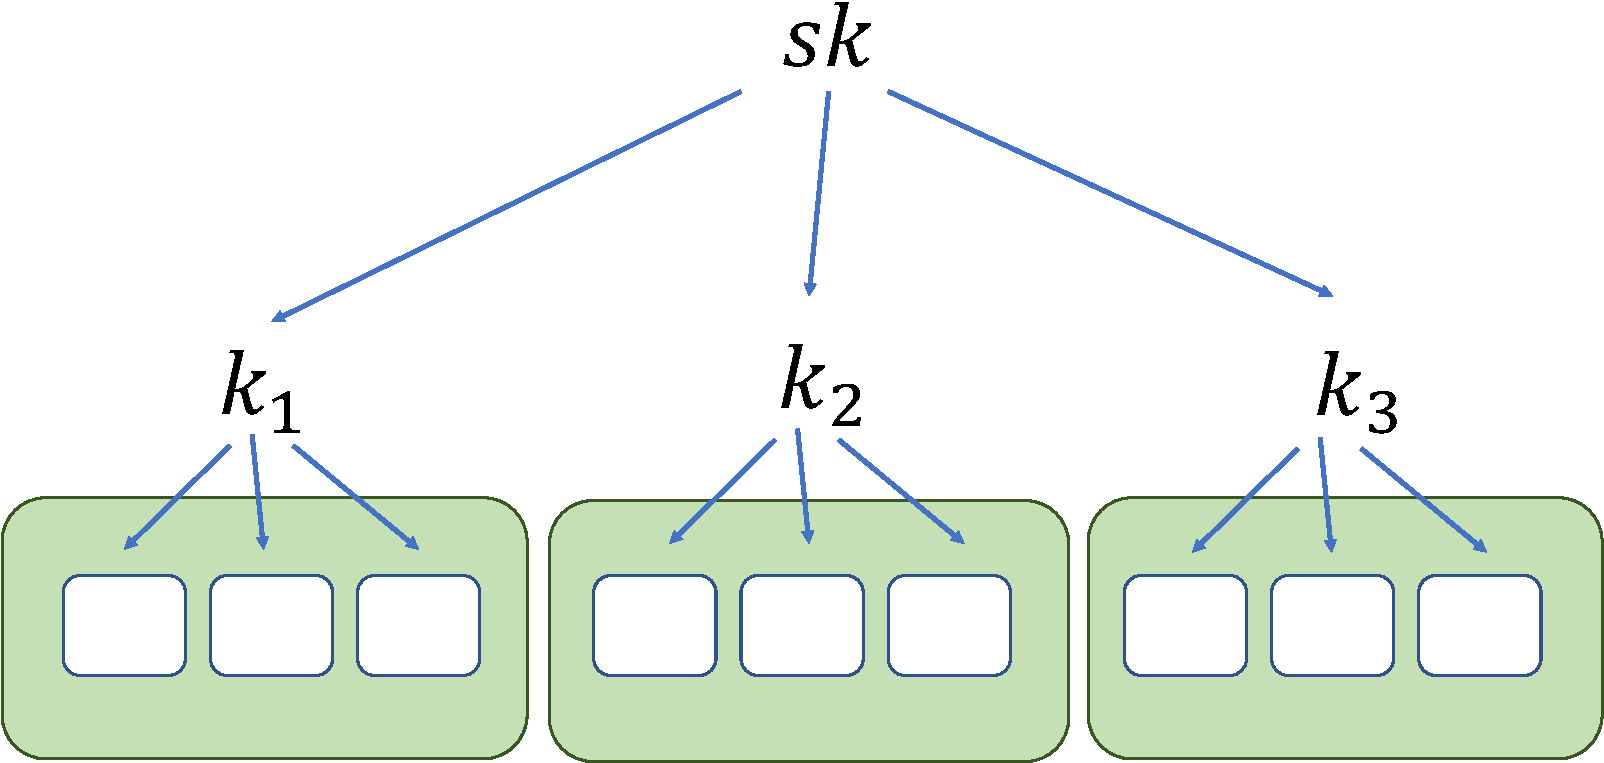
\includegraphics[width=0.6\linewidth]{figs/set-rep.pdf}
    \caption{Two-layer set representation\label{fig:set-rep}. The first layer key expands to $n^{1/4}$ sub-keys. Each sub-key controls a superblock and expands to $n^{1/4}$ offsets. Each offset in a chunk represents an index.}
\end{figure*}

%Here, $x[i:j]$ means the bit string from the $i$-th bit to the $(j-1)$-th bit of $x$'s binary representation.

Again, the high level idea behind the online query is similar: the client finds
a key $\sk$ such that $x\in \Set(\sk)$. The client wants to learn the parity of
$\Set(\sk_i)/\{x\}$. We now present in two-steps below how the two-layer set
representation helps us to reduce the online communication cost to
$\widetilde{O}_\lambda(n^{1/4})$ bits. 

\begin{itemize}
    \item \textit{Step 1: Learning the parities for all superblocks except the
    one containing $x$.}
    
    The client first expands $\sk$ to $n^{1/4}$ sub-keys,
    $k_0,\dots,k_{n^{1/4}-1}$. Now, the client replaces the $\superblock(x)$-th
    sub-key by a uniformly random sub-key $k'\getr\{0,1\}^\lambda$. This ensures
    that from the server's view, these $n^{1/4}$ sub-keys are random after the
    replacement. The client sends these $n^{1/4}$ sub-keys to the server. For
    each superblock $i$, the server will expand the $i$-th sub-key to $n^{1/4}$
    offsets and consider them as the offsets for the $n^{1/4}$ chunks in the
    superblock $i$. The server computes the parity for the $n^{1/4}$ indices
    corresponding to the offsets. Denote the parity as $\alpha_i$. The server
    returns $(\alpha_0,\dots,\alpha_{n^{1/4}-1})$ to the client. Then, except
    $\alpha_{\superblock(x)}$, all other $\alpha$ are the correct parities for
    their corresponding superblocks. The client can simply compute the xor-sum
    of those $n^{1/4}-1$ superblocks.

    \item \textit{Step 2: Learning the parity of all other indices in $x$'s
    superblock except $x$.} Now, the client expands $k_{\superblock(x)}$ to
    $n^{1/4}$ offsets, $\delta_0,\dots,\delta_{n^{1/4}-1}$. Notice that in the
    relative location of $x$'s chunk, the offset will be $x \mod \sqrt{n}$.
    Recall that the client already preprocessed polylogarithmic random
    replacement, i.e., index-value pairs in each chunk. Assume the first
    unconsumed replacement index in $x$'s chunk is $y$. The client simply
    replaces $x$'s offset to $y$'s offset and sends those $n^{1/4}$ offsets to
    the server. This ensures that from the server's view, these $n^{1/4}$
    offsets are random after the replacement. Upon receiving those offsets, the
    server does not know which superblock they correspond to. However, the
    server can just enumerate all $n^{1/4}$ possible cases: for
    $i\in\{0,\dots,n^{1/4}\}$, the server considers those $n^{1/4}$ offsets are
    the offsets of those items in the $n^{1/4}$ chunks of the $i$-th superblock,
    and computes the corresponding parity $\beta_i$. The server returns
    $(\beta_0,\dots,\beta_{n^{1/4}-1})$ to the client. The client knows that
    $\beta_{\superblock(x)}$ is the correct parity for $x$'s superblock, except
    that the index $x$ is replaced with $y$. After removing the influence of $y$
    (the client already knows $\DB[y]$), it knows the parity of those indices
    inside $x$'s superblock except $x$.

\end{itemize}

Finally, the client can learn the parity of $ \Set(\sk)/\{x\}$ by xoring the answers from step 1 and 2. Then the client can derive $\DB[x]$.
Notice that in this algorithm, the client sends $n^{1/4}$ sub-keys and $n^{1/4}$ offsets to the server, and the server returns $2n^{1/4}$ parities (bits) to the client. 
So the communication cost is $O_\lambda(n^{1/4})$.
Also, the server's computation time in both steps is simply $O_\lambda(\sqrt{n})$ without any further optimization.
We present the pseudocode for the single query algorithm in~\Cref{fig:single-query}.

\begin{figure}
    \centering
    \begin{subfigure}[b,labelformat=empty]{0.48\textwidth}
        \centering
        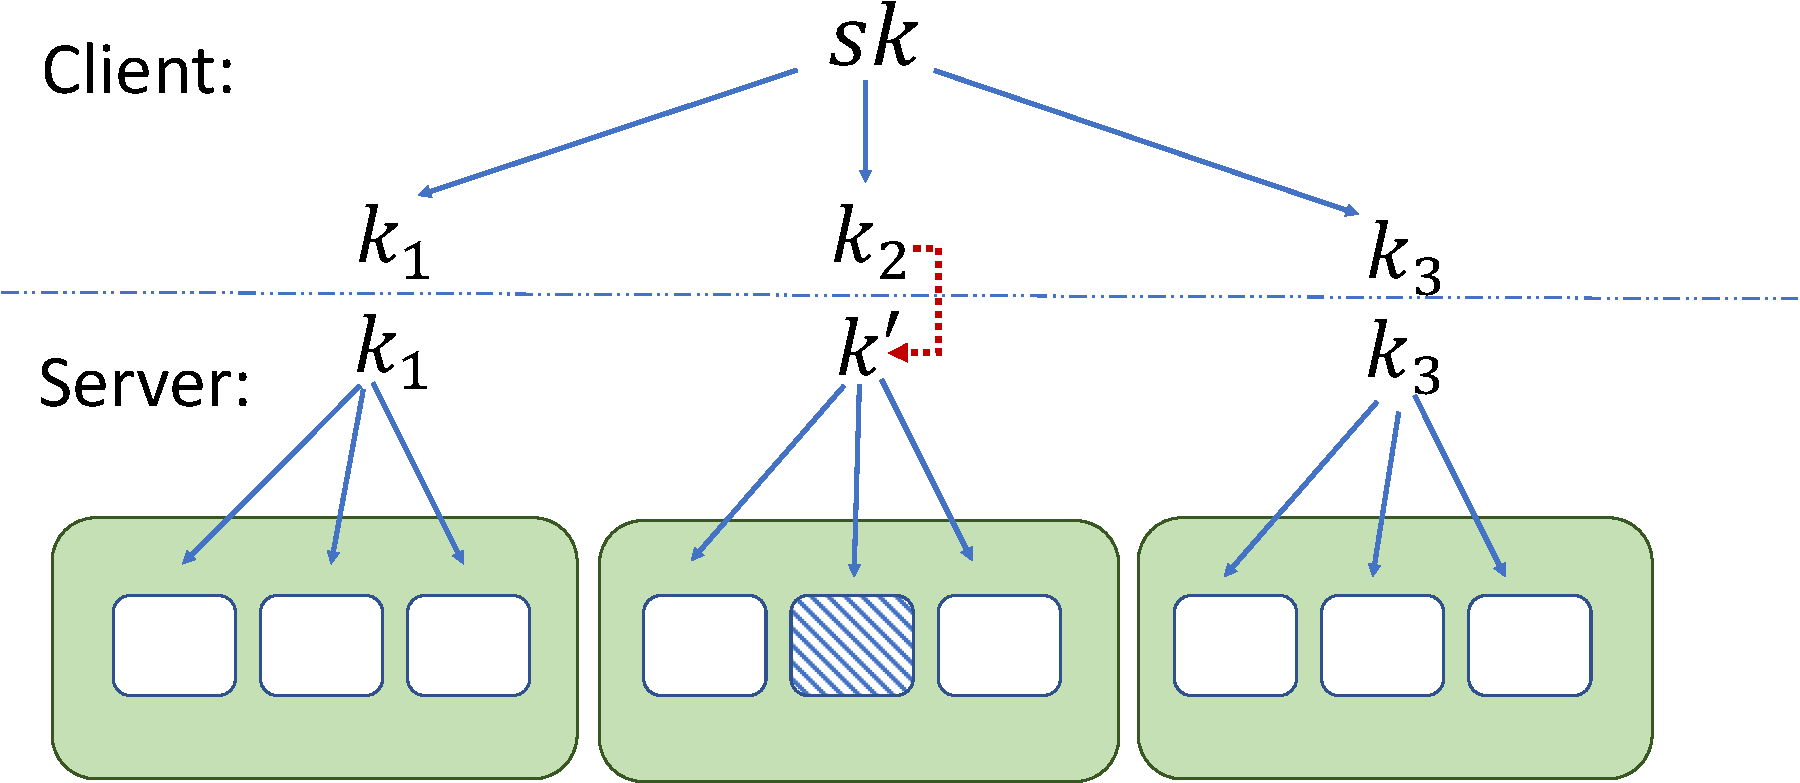
\includegraphics[width=\textwidth]{figs/step1.pdf}
        \caption*{Step 1: The client expands the main key to $n^{1/4}$ sub-keys and replaces the one that controls $x$'s superblock to a uniformly random one. The server returns $n^{1/4}$ parities for those $n^{1/4}$ superblocks.}
        % \label{fig:step1}
    \end{subfigure}
    \hfill
    \begin{subfigure}[b,labelformat=empty]{0.48\textwidth}
        \centering
        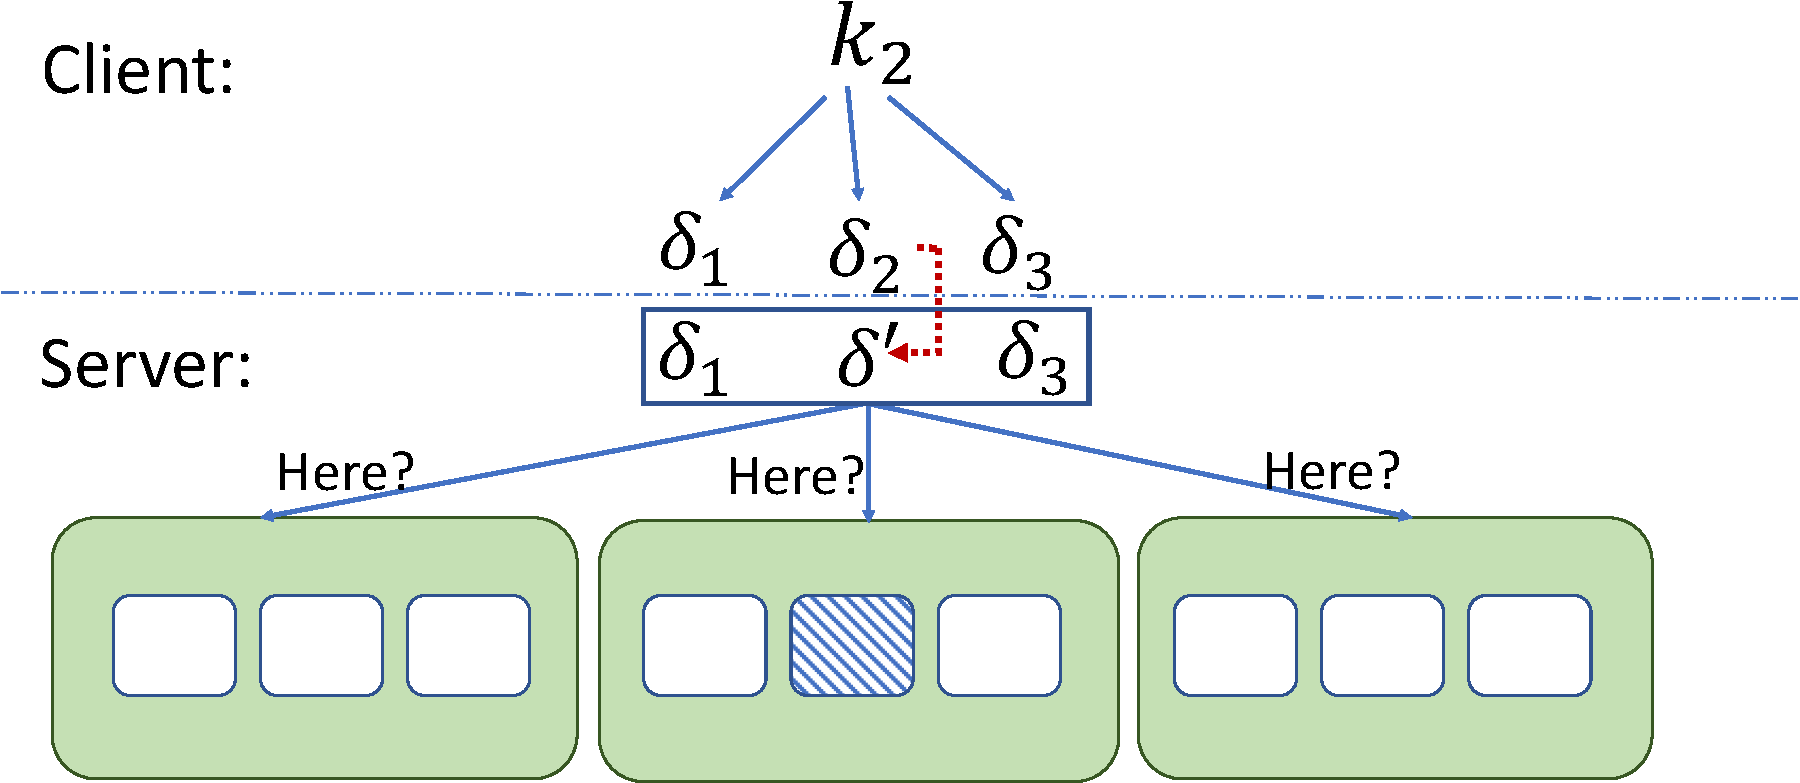
\includegraphics[width=\textwidth]{figs/step2.pdf}
        \caption*{Step 2: The client expands the sub-key to $n^{1/4}$ offsets and replaces the offset of $x$ to a random one. The server puts those offsets into every superblock. Returns $n^{1/4}$ corresponding parities. }
        % \label{fig:step2}
    \end{subfigure}
    \caption{Demonstration of the single-query algorithm assuming the query is in the middle chunk. The server does not know where the query is because the replacing operations are oblivious.}
    \label{fig:algo}
\end{figure}

%The main idea in our new construction is instead of sending over the offsets of $\sqrt{n}$ values, the client will send over $n^{1/4}$ ``sub-keys'' and $n^{1/4}$ offsets, thereby reducing the communication. The sub-keys will be $\lambda$ bits long and will correspond to a superblock. Further, a sub-key will be sufficient to compute all the offsets of a chunk in a superblock. 

%In order to read the value at index $x$, the client will compute the $n^{1/4}$ sub-keys for all the chunks, and compute all the offsets only for the chunks in same superblock as $x$ is in. The client then sends over {\bf 1)} all the sub-keys, except the one for the superblock of $x$, replacing it with a random sub-key {\bf 2)} all the offsets for the chunks in the superblock of $x$, except the offset for $\chunk(x)$, replacing it with the offset of a random element $r$ which is in $\chunk(x)$, such that $\DB[r]$ was stored during preprocessing.

%We need to specify how these sub-keys for the superblocks are computed given the $\PRF$ key. Here, we utilize the underlying structure of the $\PRF$ . We assume that the $\PRF:\bits^{\lambda}\times \bits^{\frac{\log n}{2}}\to \bits^{\frac{\log n}{2}}$ is constructed from two different $\PRF$'s $\PRF_1: \bits^{\lambda}\times \bits^{\frac{\log n}{4}}\to \bits^{\lambda},\PRF_2:\bits^{\lambda}\times \bits^{\frac{\log n}{4}}\to \bits^{\frac{\log n}{2}}$ as follows:
%\begin{align*}
%    \PRF(\sk,x)=\PRF_2(\PRF_1(\sk,x[0]),x[1])\;,
%\end{align*}
%where $x[0],x[1]$ denote the first $\frac{\log n}{4}$ and last $\frac{\log n}{4}$ bits of $x$ respectively. The GGM construction~\cite{GGM86} in particular can be viewed to be of this form.

%Given $\sk$, the sub-key for superblock $i$ is $k_i=\PRF_1(\sk,i)$ for $i\in \{0,1,\ldots,n^{1/4}-1\}$. Note that all the offsets for chunk $i$ can be computed using $k_i$. As specified above, the client sends over $n^{1/4}$ different sub-keys and $n^{1/4}$ different offsets to the server. Label the sub-keys received by the server as $k_0',k_1',\ldots,k_{n^{1/4}-1}'$ and label the offsets as $\delta_0',\delta_1',\ldots,\delta_{n^{1/4}-1}'$.

% \heading{Superblocks, sub-keys and the low bandwidth construction.} Let $x_0\in \bits^{\frac{\log n}{2}}$. Observe that, because of the property of $\PRF$, if the client provides the evaluation of $\PRF_1(\sk,x_0)$, the server can compute $\PRF(\sk,x_0\concat x_1)=\PRF_2(\PRF_1(\sk,x_0),x_1)$ for any $x_1\in \bits^{\frac{\log n}{2}}$. We use this observation to compress the online bandwidth.
% If the client wants to read the location $x$, and $\sk$ is a hint such that $x\in\Set(\sk)$, for all $y\in \{0,1,\ldots,n^{1/4}-1\}$, the client compute $\PRF_1(\sk,y)$. Let these values be $k_0,k_1,\ldots,k_{n^{1/4}-1}$ -- we refer to them as ``sub-keys''. 

% We introduce a new terminology: for every $x\in \{0,\ldots,{n}-1\}$ we say that $x$ is in the ``superblock" $j$ if $\lfloor x/n^{1/4}\rfloor = j$. Further, we say that the relative location of $\chunk(x)$ in superblock $j$ is $\chunk(x)-j\cdot n^{1/4}$. 

% We also refer to $k_j$ as the sub-key for that superblock. Let $b^*=\superblock(x)$ and $d^*$ be the relative location of $\chunk(x)$ in $\superblock(x)$, i.e. $d^*=\chunk(x)-\superblock(x)\cdot n^{1/4}$. Let $\delta_i=\PRF_2(k_{b^*},i)$ for $i\in \{0,1,\ldots,n^{1/4}-1\}$.
% Let $k'$ be a randomly sampled sub-key and let $r$ be a random value in $\{0,\ldots,n-1\}$ such that $\DB[r]$ such that $\chunk(r)=\chunk(x)$ had been read and stored by the client during the preprocessing. Let $\delta=r \text{ mod }\sqrt{n}$. The client sends over the following to the server:
% \begin{itemize}
%     \item the subkeys $k_0,\ldots,k_{n^{1/4}-1}$ \emph{except} $k_{b^*}$, replacing it with $k'$, 
%     \item the offsets $\delta_0,\ldots,\delta_{n^{1/4}-1}$ \emph{except} $\delta_{d^*}$, replacing it with $\delta'$.
% \end{itemize}

%For each $b\in \{0,\ldots,n^{1/4}-1\}$, the server computes the offsets for the $b$-th sub-key $k_b$, i.e. computes $\PRF_2(k_b',y)$ for each $y\in \{0,1,\ldots,n^{1/4}-1\}$. Assuming that this $b$-th sub-key is the sub-key for the $b$-th superblock (this assumption is correct except for the superblock $x$ is in), it computes the xor-sum of all the database entries indexed by the values in the superblock. Call this xor-sums $\alpha_b$. Next for $b\in  \{0,\ldots,n^{1/4}-1\}$, the server assumes that the offsets were of the $b$-th superblock and computes the xor-sum of the super-block accordingly (this assumption in contrast is \emph{only} correct for the superblock $x$ is in). Call the xor-sums $\beta_b$. The server sends over all the $\alpha_b$'s and $\beta_b$'s for $b\in  \{0,\ldots,n^{1/4}-1\}$ to the client.

\begin{figure}[p]
    
    \begin{minipage}{\textwidth}
        \begin{mdframed}
            \label{alg:one-query}
            \begin{center}
                {\bf Query Protocol for a Single Query $x$: $\SingleQuery(x,
                \sk, p_{\sk}, r, p_r)$.
                    %\andy{Is it not $O(\sqrt{n})$?}
                }
            \end{center}
            
            \parhead{Client's input:}
            %Suppose the client has the following inputs:
            \begin{itemize}
                \item A master PRF key $\sk$ assuming $x\in \Set(\sk)$;
                \item The parity of $\Set(\sk)$ is assumed to be $p_{\sk}$;
                \item A random index $r$ in $x$'s chunk such that the  $\DB[r]$
                is assumed to be $p_r$.
            \end{itemize}
            
            %\parhead{Suppose the client has a hint $$} When a query $x \in \{0,
            %1, \ldots, n-1\}$ arrives, \Client performs the following: 
            \begin{enumerate}[leftmargin=5mm,itemsep=1pt]
                \item 
                {\bf Step 1: (Client)}

                \begin{enumerate}[leftmargin=5mm,itemsep=1pt]
                        
                        \item Let $b^*={\sf superblock}(x)=\lfloor x/n^{3/4}
                        \rfloor, c^* = {\sf chunk}(x)=\lfloor x/n^{1/2}
                        \rfloor$. Let $d^*=\chunk(x)\mod n^{1/4}$ be the
                        relative chunk location of $x$ in the superblock. 
                        

                        \item Expand $\sk$ to $n^{1/4}$ sub-keys $k_{
                        0},\dots,k_{n^{1/4}-1}$ where $k_{b}=\PRF_1(\sk, b)$ for
                        all $b$.
                    
                        \item Expand the $b^*$-th sub-keys to $n^{1/4}$ offsets
                        $\delta_{0},\dots,\delta_{n^{1/4}-1}$ where
                        $\delta_{\ell}=\PRF_2(k_{b^*}, \ell)$.
                        
                        \item Sample a random sub-key $k'\getr\{0,1\}^\lambda$
                        and denote $\delta'=r\mod \sqrt{n}$.
                        \item Send the following tuples to the server:
                        \begin{align*}
                            (k_{0},\dots,k_{b^*-1}, k',k_{b^*+1},\dots,k_{n^{1/4}-1}) \\
                            (\delta_{0},\dots,\delta_{d^*-1},\delta' ,\delta_{d^*+1},\dots,\delta_{n^{1/4}-1})
                        \end{align*}
                    
                \end{enumerate}
                
                \newpage
                
                \item 
                {\bf Query Step 2: (Server)}
                
                Upon receving the tuples $(k'_0,\dots,k'_{n^{1/4}-1})$,
                $(\delta'_0,\dots,\delta'_{n^{1/4}-1})$: 
                \begin{enumerate}
                    \item For $b\in \{0,\dots,n^{1/4}-1\}$:
                    \begin{enumerate}
                        \item Expand $k'_b$ to $n^{1/4}$ offsets and consider
                        them being the corresponding index offsets in chunk $\{b
                        \cdot n^{1/4}, \ldots, (b + 1)\cdot n^{1/4} -1\}$.
                        Compute the xor-sum of the database values for those
                        indices as 
                        \[
                        \alpha_b=\xor_{c\in \{0,\dots,n^{1/4}-1\}} \DB[(c + bn^{1/4})\sqrt{n} + \PRF_2(k'_b, c)].
                        \]
                        \item Consider $(\delta'_0,\dots,\delta'_{j,n^{1/4}-1})$
                        as the corresponding index offsets in chunk $\{b \cdot
                        n^{1/4}, \ldots, (b + 1)\cdot n^{1/4} -1\}$. Compute the
                        xor-sum of the database values for those indices as 
                        \[
                        \beta_b=\xor_{c\in \{0,\dots,n^{1/4}-1\}} \DB[(c + bn^{1/4})\sqrt{n} + \delta_c].
                        \]
                    \end{enumerate}
                    
                    \item Return $(\alpha_0,\dots,\alpha_{n^{1/4}-1}),
                    (\beta_0,\dots,\beta_{n^{1/4}-1})$ to the client.
                \end{enumerate}
                
                
                \item 
               {\bf Step 3: (Client)}
               
               Upon receiving $(\alpha_0,\dots,\alpha_{n^{1/4}-1}),
               (\beta_0,\dots,\beta_{n^{1/4}-1})$:
                \begin{itemize}[leftmargin=5mm,itemsep=1pt]
                    \item 
                    The xor-sum of the items in $\Set(\sk)$ except those in the
                    superblock of $x$ is
                    $\alpha=\sum_{b\in\{0,\dots,n^{1/4}-1\},b\ne b^*}\alpha_b$.
                    
                    \item The xor-sum of the items in the superblock of $x$
                    except $x$ is $\beta=\beta_{b^*}\xor p_r$.
                    
                    \item Then, the value of $x$ is
                    $\DB[x]=p_\sk\xor\alpha\xor\beta$.
                \end{itemize}
            \end{enumerate}
        \end{mdframed}
    \end{minipage}
    \caption{Query Protocol for a single query that reduces communication to
    $O(n^{1/4})$. This is used as a sub-routine in the sublinear single server
    PIR scheme presented in Section~\labelcref{sec:nquarter}.}
    \label{fig:single-query}
\end{figure}



%Given all the $\alpha_b$'s the client can compute the xor sum of all the values
% indexed by $\Set(\sk)$, except for those in superblock of $x$. From the
% preprocessing the client knows the xor-sum of all the values indexed by
% $\Set(\sk)$ and thereby can compute the xor-sum of all the values indexed by
% the elements in the super-block of $x$. Further, the $\beta_b$'s along with
% the value of $\DB[r]$ for the $r$ client used specify can be used to compute
% $\DB[x]$ from the  xor-sum of all the values indexed by the elements in the
% super-block of $x$. Now, suppose $b^*=\superblock(x)$. Observe that $\alpha=
% \alpha_{b^*}\oplus \sum_{i=0}^{n^{1/4}-1}\alpha_i$ is the xor-sum of the
% database entries indexed by all the values at all the super blocks except
% super-block $b^*$. Further, $\beta=\beta_{b^*}\oplus p_r$ (where $p_r=\DB[r]$,
% the value of the database at $r$, which was stored by the client during
% preprocessing) is the xor-sum of all the entries of the database indexed by
% the values in the super-block $b^*$ except the value indexed by
% $\delta_{d^*}$. If $p_{\sk}$ was the parity of all the bits of the database
% indexed by $\sk$ (that the client stored during preprocessing), it follows
% that $\DB[x]=p_{\sk}\oplus\alpha\oplus \beta$. The client can compute this
% since it has stored $p_r,p_{\sk}$ during preprocessing and received rest of
% the values from the server.


\subsection{Supporting multiple queries in the online phase} 

Thus far, we have
given a new, low-communication protocol that handles only one query. We now want
to make $Q=\sqrt{n}/2$ queries with just one offline phase. For convenience, we
first make some assumptions about the queries without loss of generality, which
are also made in $\Piano$:
\begin{itemize}
    \item \textit{The client does not make repeated queries.} This can be ensured 
    by requiring the client to store a local cache of size $Q$ for caching the
    most recent $Q$ queries. If the client wants a repeated query, it can lookup
    in the cache and make a dummy query.
    
    \item \textit{The queries the client makes are on random indices.} This is a relatively
    strong assumption. However, we argue that it can be made without loss of
    generality and can be done by letting the client and the server agree on a
    pseudorandom permutation (PRP)~\cite{prp1,prp2} upfront and the server can
    permute the database according to the PRP. Another option is let the server
    build the database as a key-value storage and use a cuckoo hash
    table~\cite{cuckoo1,cuckoo2} directly based on a PRF to locate the queries.
    Notice that, in both implementations, the client can still make queries
    adaptively depending on the real query sequnce and the responses, which is
    sufficient for practical usage. Then, as long as the client makes the
    queries independent of the randomness of the PRP/PRF, those queries can be
    considered as uniformly random. This assumption is only needed for the
    correctness.
\end{itemize}

In order to support multiple queries, the key idea that had been used in
$\Piano$ was to ``refresh" the consumed hint by re-programming a fresh hint in a
way that does not change the distribution of the hints. Here, while our high
level goal will be the same, our strategy to do it would be significantly
different. The reason why the approach used in $\Piano$ does not translate here
is because of the following tension. Since in this new protocol we compress
bandwidth by making the client send only \emph{sub-keys} for the superblocks,
re-programming the hint while still having this compression would make
distribution of the client's future messages depend on the current query, which
violates privacy. Therefore, we seem to require newer ideas to avoid this issue.


Our main idea here is that when the client wants to read $x$, they find
\emph{all} the hints $\sk_i$ such that $x\in\Set(\sk_i)$. The client then runs
the single query protocol based on all of these hints\footnote{To ensure privacy, we
will have an probabilistic upper bound on how many queries are made. If the
client does not have that many hints, it pads some dummy queries.}. After these
hints have been consumed, the client needs to generate new hints so that the
distribution of local hints does not change. Here, for each consumed hint, the
client resamples a new key $\sk$ such that $x\in \Set(\sk)$ by rejection
sampling\footnote{The reason why the client cannot replace those hints with a
uniformly random one is that the occurrence of $x$ in the remaining tables are
less likely, and thus skewing the distribution.}. However, this could raise of
problem of ``broken hints'': the client does not know the parity for these newly
generated sets, and thus these new hints are marked as ``broken''. 

The key observation is this: as long as there is at least one non-broken hint
among the chosen hints, then the client can \emph{still} find the right
$\DB[x]$. And we will prove that except with negligible probability, at least
one of the hints for $x$ that the client chooses is not broken. Moreover, the
client only needs to consume the replacement index-value pairs for that single
query based on the one non-broken hint. For every other queries, the client does
not care about the response, so the client just replaces $x$'s offset with a
random offset. Notice that if the client shuffles the order of queries, the
query based on good hint and the queries based on the broken hints are
identically distributed from the server's view. Lastly, we argue that the client needs running time roughly $O(\sqrt{n})$ trials to rejection sample one hint in expectation. This follows since if we sample a random secret key
$\sk$, the probability that $\PRF(\sk,\chunk(x))=x-\chunk(x)\cdot \sqrt{n}$ is
$\Theta(1/\sqrt{n})$ assuming that the $\PRF$ was a random function. There are superlogarithmically many hints that need to be sampled.
This can be done in $\widetilde{O}(\sqrt{n})$ expected
time.

\begin{figure}[p]
    \begin{minipage}{\textwidth}
        \begin{mdframed}
            \label{alg:fullpolyl}
            \begin{center}
                {\bf Single-Server Scheme for $Q=\sqrt{n}/2$ Queries
                    \footnote{For clarity, we present the scheme supporting distinct and random queries. As mentioned before, these restrictions can be removed by applying PRP and local caching.}
                }
            \end{center}
            \parhead{Notation.}
            $\kappa$ denotes a {\it statistical} security parameter, $\lambda$
            denotes a computational security parameter. We use $\alpha(\kappa)$
            to denote an arbitrarily small super-constant function.

           \parhead{Offline preprocessing.} 
            \begin{itemize}[leftmargin=3mm,itemsep=1pt]
                \item 
                \Client samples $M_1=2\sqrt{n}\log \kappa \cdot \alpha(\kappa)$
                master PRF keys denoted $\psk_1, \dots, \psk_{M_1} \in \{0,
                1\}^\lambda$ for the primary table.
                %, where $M_1=\sqrt{n}\log \kappa \cdot \alpha(\kappa)$. , such
                %that $\alpha(n)=\omega(1)$. \elaine{TODO: fix params}
                Initialize the parities $p_1,\dots,p_{M_1}$ to zeros.
                
                %\elaine{TODO: notation inconsistent with earlier text}
                
                \item 
                \Client downloads the whole DB from the server in a streaming
                way: when the client has the $j$-th chunk
                $\DB[j\sqrt{n}:(j+1)\sqrt{n}]$:
                \begin{itemize}
                    \item {\it Update primary table}: for $i \in [M_1]$, let
                    $p_i \get p_i \oplus \DB[\Set(\psk_i)[j]]$.
                    \item {\it Store replacement entries}: sample and store
                    $M_2=3\log \kappa \cdot \alpha(\kappa)$ % \log \kappa\cdot
                    % \alpha(\kappa)$ 
                    tuples of the form $(r, \DB[r])$ where $r$ is a random index
                    from the $j$-th chunk.
                    %independent random indices from $[i\sqrt{n}:(i+1)\sqrt{n}]$
                    %with the associated database values.
                    \item Delete $\DB[j \sqrt{n}:(j +1)\sqrt{n}]$ from the local
                    storage.
                \end{itemize}
                
                \item At this moment, let $T := \{(\psk_i, p_i )\}_{i \in
                [M_1]}$ denote the client's {\it hint table}. Mark all the hints
                as ``good''.
            \end{itemize}
            
            
            
            
            \parhead{Online query for index $x \in \{0, 1, \ldots, n-1\}$.}
            %When a query $x \in \{0, 1, \ldots, n-1\}$ arrives, \Client
            %performs the following: 
            \begin{enumerate}[leftmargin=5mm,itemsep=1pt]
                \item 
                {\bf Query:}
                \begin{enumerate}[leftmargin=5mm,itemsep=1pt]
                    %\item Let %$i^*=\left\lfloor
                    %\frac{x}{\sqrt{n}}\right\rfloor$ be the index of $x$'s
                    %chunk.
                    \item 
                    \Client finds all the matched hints
                    $(\sk_1,p_1),\dots,(\sk_m,p_m)$ in the hint table  such that
                    $x\in \Set(\sk_j)$ for all $j\in[m]$.
                    
                    \item 
                    If there are less than $M_3=6(\ln \kappa \alpha(\kappa))^2$
                    hints, pad them with random broken hints. If there are more
                    than $M_3$ hints, sample $M_3$ hints from them. Randomly
                    shuffle the order of these hints\footnote{We add this random
                    shuffle to ensure that the order of the hints do not reveal
                    any information}.
                    %\item If there are more than $M_3$ matched hints, randomly
                    %choose $M_3$ hints among them. (see \Cref{eqn:setfromkey}
                    %for the definition of $\Set(\psk_j, x')$ where $x'$ is
                    %possibly $\bot$). 
                    
                    
                    % \item For the one of the randomly chosen good matched hint
                    % $(\sk_j, p_j)$\footnote{If there are no good matched hint,
                    % just mark the answer as 0.}:
                    % \begin{itemize}
                    %     \item \Client finds the first unconsumed replacement
                    %     entries $(r, \DB[r])$ from $x$'s chunk;
                    %     \item Execute $\SingleQuery(x, \sk_j, p_j, r, \DB[r])$
                    %     and mark the answer for the query.
                    % \end{itemize} 
                    
                    % \item Simultaneously, for other matched hints $(\sk_j,
                    % p_j)$: 
                    % \begin{itemize}
                    %     \item \Client executes $\SingleQuery(x, \sk_j, 0, r',
                    %     0)$ with a random index $r'$ from $x$'s chunk and
                    %     ignores the answer.
                    % \end{itemize}
                    \item For each hint, do the following:
            \begin{itemize}
                \item if the hint is marked good, find the first unconsumed replacement entry $(r, \DB[r])$ from $x$'s chunk;
                and execute $\SingleQuery(x, \sk_j, p_j,r,\DB[r])$ and store the answer for the query.
                \item Otherwise, execute $\SingleQuery(x, \sk_j, 0,0,r')$ with a random index $r'$ from $x$'s chunk  and ignore the answer.
            \end{itemize}
                
            \item Return the answer of any of the good hints. If none of the hints were good, just return $0$.
                    
                \end{enumerate}
                
                \item 
                {\bf Refresh:}
                \begin{itemize}
                    \item \Client replaces all the keys for the matched hints in
                    the hint table with $\sk'_1,\dots,\sk'_m$, such that for all
                    $j$, $\sk'_j$ is rejection-sampled conditioned on $x\in
                    \Set(\sk'_j)$. Also mark the parities as 0 and mark those
                    hints as ``broken''.
                \end{itemize}
                
            \end{enumerate}
        \end{mdframed}
    \end{minipage}
    \caption{Sublinear single server preprocessing PIR protocol introduced in
    Section ~\labelcref{sec:single-server}. The protocol uses $\SingleQuery$ defined
    in Fig.~\labelcref{fig:single-query} as a sub-routine.}
    \label{fig:single-server}
\end{figure}


\ignore{

To sum up the major changes in this construction compared to $\Piano$ are the
following.
\begin{itemize}
    \item Instead of sending over all the $n^{1/2}$ indices, the client sends
    $n^{1/4}$ sub-keys and $n^{1/4}$ offsets.
    %\item The preprocessing does not store backup hints for each chunk, instead
    %storing a super logarithmic number of random values $r$ and $\DB[r]$ for
    %each chunk.
    \item When querying $x$, online phase runs the protocol for single reads for
    all matched hints instead of just for the first one as in $\Piano$. At the
    end the client chooses the correct answer appropriately.
    \item When replacing a hint that was consumed for $x$, the client simply
    rejection samples a new hint, sets its parity to $0$ and marks it as broken.
\end{itemize}

}


\subsection{Putting everything together in the two-server setting}



So far we have been focused on the online phase.
We now introduce the implementation of the offline phase.

In the two-server setting, we assume there are two non-colluding servers and each one of them stores a replica of the database.
We call them the left server and the right server for convenience.

In fact, in the two-server setting, handling the offline phase is straightforwad.
After the client generates all $M_1=\widetilde{O}_\lambda(\sqrt{n})$ keys, 
the client will directly send the keys to the left server the left server expands those keys 
to sets.
Then, the left server returns the parities of those sets to the client.
Moreover, the client will sample polylogarithmic random indices in each chunk
and directly ask the left server about their values.
Then, the client only interacts with the right server during the online phase, just as the protocol we mentioned before.

We omit the pseudocode for the two-server version, which will be nearly the same as the single-server version presented later in~\Cref{fig:single-server}. 

\begin{theorem}
    Let $\lambda,\kappa\in \mathbb{N}$.
    Let $\alpha(\kappa)$ be any superconstant function. Assume $\PRF_1,\PRF_2$ is secure pseudorandom functions. Assume $n$ is bounded by $\poly(\lambda)$ and
    $\poly(\kappa)$. The two-server PIR scheme that supports $Q=\sqrt{n}/2$ queries is private, correct with probability
    $1-\negl(\lambda)-\negl(\kappa)$ where $\negl(.)$ is a negligible function. Further, it achieves the following performance
    bounds:
    
    
    \begin{itemize}
        \item $O(\lambda\sqrt{n}\log \kappa \alpha(\kappa))$ client storage and
        no additional server storage;
        \item \textbf{Offline Phase}:
        \begin{itemize}
            \item $O(\lambda n\log \kappa \alpha(\kappa))$ server time and
            $O(\lambda\sqrt{n}\log \kappa \alpha(\kappa))$ client time;
            \item \underline{$O(\lambda\sqrt{n}\log \kappa \alpha(\kappa))$
                communication}.
        \end{itemize}
        \item \textbf{Online Phase}:
        \begin{itemize}
            \item $O(\lambda\sqrt{n}\log \kappa \alpha(\kappa))$ expected client
            time and $O(\lambda\sqrt{n}(\log \kappa \alpha(\kappa))^2)$ server
            time per query; 
            \item $O(\lambda n^{1/4}(\log \kappa    \alpha(\kappa))^2)$
            communication per query.
        \end{itemize}
    \end{itemize}     
\end{theorem}

\subsection{Putting everything together in the single-server setting}

\label{sec:single-server}

In the single-server setting, we have to ensure that the preprocessing is server-oblivious to get privacy.
We can follow the same idea from $\Piano$~\cite{piano} such that the client downloads the whole database to do the preprocessing in a streaming fashion. 
    The client initializes all the hints and updates the hints along with the streaming.
    After the client completes the preprocessing, it interacts with the server during the online phase.
    To the server, the offline phase is oblivious, so this scheme is also private. 
    However, now the scheme has $O(n)$ offline communication cost, and the amortized offline communication cost per query will be $O(\sqrt{n})$, instead of $\widetilde{O}_\lambda(1)$ in the two-server setting.

We give a pseudocode description of the protocol for $Q=\sqrt{n}/2$ queries in the single-server setting in
Figures~\labelcref{fig:single-server}. 

%The corollary below follows from Theorem~\labelcref{thm:main1} and the above remarks.



\begin{theorem}
    \label{thm:main1} Let $\lambda,\kappa\in \mathbb{N}$.
    Let $\alpha(\kappa)$ be any superconstant function. Assume $\PRF_1,\PRF_2$ are secure pseudorandom functions. Assume $n$ is bounded by $\poly(\lambda)$ and
    $\poly(\kappa)$. The single-server scheme in~\Cref{fig:single-server} that supports
    $\sqrt{n}/2$ queries is private, correct with probability
    $1-\negl(\lambda)-\negl(\kappa)$ where $\negl(.)$ is a negligible function. Further, it achieves the following performance
    bounds:
    \begin{itemize}
        \item $O(\lambda\sqrt{n}\log \kappa \alpha(\kappa))$ client storage and
        no additional server storage;
        \item \textbf{Offline Phase}:
        \begin{itemize}
            \item $O(n)$ server time and $O(\lambda n\log \kappa \alpha(\kappa))$ client time
            ;
            \item \underline{$O(n)$ communication};
        \end{itemize}
        \item \textbf{Online Phase}:
        \begin{itemize}
            \item $O(\lambda\sqrt{n}\log \kappa \alpha(\kappa))$ expected client
            time and $O(\lambda\sqrt{n}(\log \kappa \alpha(\kappa))^2)$ server
            time per query; 
            \item $O(\lambda n^{1/4}(\log \kappa \alpha(\kappa))^2)$
            communication per query.
        \end{itemize}
    \end{itemize} 
\end{theorem}

\begin{proof}[Proof to~\Cref{thm:main1} and~\Cref{thm:main2}]
    
    We defer the privacy and the correctness proof to~\Cref{sec:proof}.

    The client only stores $M_1=2\sqrt{n}\log \kappa\alpha(\kappa)$
    $\lambda$-bit keys and store in total $\sqrt{n}\cdot M_2=3\sqrt{n}\log
    \kappa\alpha(\kappa)$ index-value pairs. So the storage is
    $O(\lambda\sqrt{n}\log \kappa \alpha(\kappa))$.
    
    The offline performance bounds follow straightforward by the algorithm descriptions.
    
    For the online phase, the client first enumerates all $M_1$ hints to find
    $x$, which takes $O(\lambda\sqrt{n}\log \kappa\alpha(\kappa))$ time. For all
    the $M_3=\Theta((\log \kappa \alpha(\kappa))^2)$ found hints, the
    $\SingleQuery$ algorithm takes $O(\lambda n^{1/4})$ client computation and
    $O(\lambda \sqrt{n})$ server computation, while the communication cost is $O(\lambda
    n^{1/4})$. During the refresh phase, we consider the expected computation time: each hint in the table will have $1/\sqrt{n}$ probability to be resampled and each resample takes $O(\lambda\sqrt{n})$ expected time to finish. 
    So the total expected time for the online phase is $O(\lambda\sqrt{n}\log \kappa
    \alpha(\kappa))$  per query. The online server time is
    $O(\lambda\sqrt{n}(\log \kappa \alpha(\kappa))^2)$ per query. The online
    communication per query is $O(\lambda n^{1/4}(\log \kappa
    \alpha(\kappa))^2)$.
\end{proof}



\paragraph{Supporting unbounded number of queries.}
The aforementioned scheme supports $Q=\sqrt{n}/2$ queries. 
We need a scheme that supports unbounded number of queries. 
We discuss different options below.

\begin{itemize}
    \item \textit{Repeating the $Q$-query scheme}. 
    The straightforward way is that once the client finishes a window of $Q$ queries, the client and the server(s) rerun the preprocessing phase again, using fresh randomness. 
    The drawback is that the client has to wait a long time before starting the next window.
    
    \item \textit{Pipelining the proprocessing and online phase}.
    It follows the same idea as in $\Piano$~\cite{piano}.
    The scheme first runs a preprocessing phase for the first $Q$ queries. 
    Then, during the online phase, the client interacts with the preprocessing server and gradually finishes the preprocessing for the next $Q$ queries. 
    Essentially, the client and the server can split the work (including computation and communication) of the preprocessing into $Q$ pieces.
    Whenever the client finish a query, the client and the preprocessing server will finish the next piece of work about preprocessing.
    Once the client finishes the $Q$ queries, it can immediately starts the next window of $Q$ queries because the preprocessing for the next window is done. 
    The main advantage is that the client never waits long time after the first preprocessing phase.
    The downside is: 1) in the two server setting, it requires the preprocessing server to be always online; 2) in the single-server setting, the online communication will be dominated by the preprocessing parts and become $O(\sqrt{n})$, instead of $\widetilde{O}_\lambda(n^{1/4})$.
\end{itemize} 






%Suppose the client has the master PRF key $\sk$ such that 



\subsection{Removing multiple $\SingleQuery$ executions via online resampling}

%\label{sec:optimized}


In the schemes mentioned in~\Cref{sec:main-scheme}, each online query will need
$6(\ln \kappa \alpha(\kappa))^2$ calls to the subroutine, $\SingleQuery$, and
each routine needs $O(\lambda n^{1/4})$ communication cost. In this section, we
introduce a slightly more involved scheme that requires \textbf{only one} call
to the $\SingleQuery$ subroutine per query.

\paragraph{Why previous schemes do not worry about broken hints.} First, we need
to understand why in the previous schemes like $\Piano$~\cite{piano}, the client
does not have to worry about broken hints. To ensure all hints are useful, the
client will prepare polylogarithmic backup hints for each of the $\sqrt{n}$
chunks. The backup hints for the $i$-th chunk will record the parity of the set
and also the value of the item in the $i$-th chunk. After querying for $x$, the
client will replace the consumed hint with a backup hint from $x$'s chunk and
replace that $i$-th element of the hint to the current query $x$, which
maintains the distribution of the hint table. Since the values for the original
$i$-th element and $x$ are known to the client, the correct parity for the
edited hint can be derived by the client locally and the new hint will always be
good. Then, the client only needs to find the first hint that contains $x$,
instead of finding all matched hints and making multiple queries based on those
hints, hoping that one of them will be good.~\footnote{A natural question is why
the client cannot simply pick the first good hint. Observe that it would be
equivalent to deleting a consumed hint from the table because a broken hint will
never be used again. Then, it would skew the distribution of the hint table
because the remaining hints are  less likely to contain the past queries, which
leads to privacy leakage.}

Notice that the hint replacement operation in $\Piano$ is done \textbf{lazily
and obliviously}: the client only stores the PRF key and the replacement
location, and only replaces the element when expanding the PRF key to a full set
of size $\sqrt{n}$ during the online query. The replacement operation is
oblivious to the server because the client will send all $\sqrt{n}$ indices to
the server, and swapping out one index with another one locally leaves no trace
of which index being replaced!

Unfortunately, this is not straightforward if we send the whole set to the
server and optimize the communication cost to $\widetilde{O}(n^{1/4})$.
%Remember that the client will send $n^{1/4}$ sub-keys to the server.
One way to achieve that is by ```programming'': when we promote a backup hint to
the primary hint table after a query, we somehow \textbf{program} the PRF
$\sk'$, so that the result of evaluating $\sk'$ on $x$'s chunk index is enforced
to be $x$'s offset. Also, the programmed PRF key should not leak the information
about which location has been programmed. Indeed, this is exactly the idea in
two previous single-server PIR schemes~\cite{pir-ec23,lazza-pir}, where they
utilized a heavy cryptographic construction called privately programmable
pseudorandom function (PPPRF) to achieve such programming operation. However,
this primitive is only known under strong cryptographic assumptions like LWE. 

\paragraph{Our solution: rejection sampling.} 
We observe that all we need to do is just to ``maintain'' the right distribution
of the hint table and the keys sent to the server. Then, we can rejection-sample
the PRF keys according to the right distribution and avoid the burden of doing
difficulty of doing private programming on the key level.

Maintaining the distribution for the local hint table is relatively simple. For
the local hint table, what we actually care about is the distribution of the
actual sets, regardless how we represent them. Assume that the client already
queries for $y$ and knows $\DB[y]$. Now the client consumes a hint that contains
$y$, and replaces it with a hint from those backup hints prepared for
$\chunk(y)$. Suppose the key for the backup hint is $\sk$. $\sk$ may not contain
$y$, but we can mark $y$ alongside the key, such that whenever we use the hint
later, we will manually enforce $y$ into the set.
\begin{figure}[p]
    
    \begin{minipage}{\textwidth}
        \begin{mdframed}
            \label{alg:optimized:full}
            \begin{center}
                {\bf Optimized Single-Server Scheme for $Q=\sqrt{n}/2$ Queries
                    \footnote{For clarity, we present the scheme supporting distinct and random queries.}
                }
            \end{center}
            \parhead{Notation.}
            $\kappa$ denotes a {\it statistical} security parameter, $\lambda$
            denotes a computational security parameter. We use $\alpha(\kappa)$
            to denote an arbitrarily small super-constant function.
            
            
            \parhead{Offline preprocessing.} 
            %\ \\[-6pt]
            \begin{itemize}[leftmargin=3mm,itemsep=1pt]
                \item In addition to the previous algorithm:
                \begin{itemize}
                    \item \Client samples $M_2=3\log \kappa \alpha(\kappa)$
                    backup keys $\sk_{i,1},\dots,\sk_{i,M_2}$ for chunk $i$;
                    \item For each backup hint, \Client stores $\sk_{i, j}$ and
                    the following information:
                    \begin{itemize}
                        \item The parity for the whole set: $p_{i,j}=\xor_{x\in
                        \Set(\sk_{i,j})} \DB[x]$;
                        \item The parity for those items within the superblock
                        that contains the $i$-th chunk: $b_{i,j}=\xor_{x\in
                        \Set(\sk_{i,j})} \I\left[\superblock(x) = \left\lfloor
                        \frac{i}{n^{1/4}} \right\rfloor
                        \right]\DB[x]$\footnote{$\I[A]$ is 1 when $A$ is true
                        and 0 otherwise.}
                       
                        \item The DB-value of the $i$-th item:
                        $\DB[\Set(\sk_{i,j})[i]]$. 
                    \end{itemize}
                \end{itemize}  
                
                             
                %\item At this moment, let $T := \{(\psk_i, p_i )\}_{i \in
                %[M_1]}$ denote the client's {\it hint table}. Mark all the
                %hints as ``good''.
            \end{itemize}
            
            
            
            
            \parhead{Online query for index $x \in \{0, 1, \ldots, n-1\}$.}
            %When a query $x \in \{0, 1, \ldots, n-1\}$ arrives, \Client
            %performs the following: 
            \begin{enumerate}[leftmargin=5mm,itemsep=1pt]
                \item 
                {\bf Query:}
                \begin{enumerate}[leftmargin=5mm,itemsep=1pt]
                    %\item Let %$i^*=\left\lfloor
                    %\frac{x}{\sqrt{n}}\right\rfloor$ be the index of $x$'s
                    %chunk.
                    \item 
                    \Client finds {the first} matched hint $(\sk_i, p_i)$
                    such that $x\in \Set(\sk_i)$ and the hint does not have a
                    positive constraint $y$ that $\chunk(y)=\chunk(x)$.

                        \item If there is no positive constraint on this hint:
                        execute $\SingleQuery$ as before (consuming a
                        replacement entry from $\chunk(x)$).
                        \item  If there is a positive constraint $+y$ on this
                        hint: 
                        \begin{enumerate}
                            \item If $\superblock(y)=\superblock(x)$, execute
                            $\SingleQuery$ as before, except:
                            \begin{itemize}
                                \item After expanding the sub-key to $n^{1/4}$
                                offsets, replace the $(\chunk(y) \mod
                                n^{1/4})$-th offset with $y$'s offset; 
                                \item If the return value is $v$, mark the
                                answer as $v\xor\DB[y]\xor
                                \DB[\Set(\sk_i)[\chunk(y)]]$. 
                            \end{itemize}

                           \item If $\superblock(y) \ne \superblock(x)$, execute
                           $\SingleQuery$ as before, except:
                           \begin{itemize}
                               \item After expanding $\sk_i$ to $n^{1/4}$
                               sub-keys, replace the $\superblock(y)$-th key
                               with a rejection-sampled key $k'$. The rejection
                               sampling key $k'$ should satisfy all constraints
                               related to the matched hint $(+y,
                               -z_1,\dots,-z_t)$ if $k'$ controls
                               $\superblock(y)$ (as specified in
                               Section~\labelcref{sec:optimized}).
                               
                               \item If the return value is $v$, mark the answer
                               as $v\xor\beta_{\superblock(y)}\xor b$, where
                               $\beta_{\superblock(y)}$ is the corresponding
                               parity of superblock controled by the
                               rejection-sampled sub-key and $b$ is the original
                               parity for that superblock, known by
                               preprocessing. 
                           \end{itemize}
                           
                            
                        \end{enumerate}
                                    
                \end{enumerate}
                
                \item 
                {\bf Refresh:}
                \begin{itemize}
                    \item \Client adds the constraint $-x$ for the first $i-1$
                    entries.
                    \item \Client replaces the matched hint with an unconsumed
                    hint from the $\chunk(x)$'s backup hint group. Clean all
                    other constraints and only mark $+x$ for the $i$-th entry.
                \end{itemize}
                
            \end{enumerate}
        \end{mdframed}
    \end{minipage}
    \caption{The optimized sublinear single server preprocessing PIR protocol
    introduced in Section ~\labelcref{sec:optimized}. The protocol uses
    $\SingleQuery$ defined in Fig.~\labelcref{fig:single-query} as a
    sub-routine.}
    \label{fig:optimized:single-server}
\end{figure}


The more tricky case is how we handle the keys that the client send to the
server. Suppose client is now querying for $x$, and it finds the first hint that
contains $x$. Also, it notices that the hint is marked with $y$. Recall that in
the $\SingleQuery$ algorithm the client will expand the master key into
$n^{1/4}$ keys and expand the keys corresponding to the superblock of $x$ to
$n^{1/4}$ offsets. Now there are two cases:
\begin{enumerate}
    \item \textit{$x$ and $y$ are in the same superblock.} This is a relatively
    simple case. We will always replace the sub-key corresponding to the
    superblock of $x$ (the same as $y$) with a uniformly random sub-key. Then,
    when we expand the original sub-key to $n^{1/4}$ offsets, we need to replace
    $x$'s offset with a random one, and also manually set the offset
    corresponding to $y$'s chunk to $y$'s offset, reflecting that we enforce $y$
    to be included in this hint. No rejection sampling is required in this case.
    
    For the answer, since we are just replacing the element in $y$'s chunk to
    $y$, the influence of such change should be removed. We can require the
    client to store the database value for the $i$-th element for all the backup
    hints dedicated for the $i$-th chunk. Then, if this promoted hint $\sk$ is
    used, we can correct the answer by xoring the influnce value,
    $\DB[\Set(\sk)[\chunk(y)]]\xor\DB[y]$.
    
    \item \textit{$x$ and $y$ are in the different superblocks.} This is the
    more involved case. We will again replace the sub-keys corresponding to
    $x$'s superblock with a uniformly random sub-key and replace the offsets in
    $x$'s chunk with a random one. However, we need to ensure that the key
    corresponding to $y$'s superblock will expand to the correct offset for
    $y$'s chunk, to ensure that $y$ is included. Now, we will rejection-sample a
    sub-key $k$ for $y$'s superblock, such that it expands to the correct offset
    of $y$. This is what we refer to as a \textbf{positive} constraint, and we
    write this constraint as $+y$.
    %We identify that this is \textbf{not enough} to ensure privacy.
    Additionally, to maintain the right distribution, there are also
    \textbf{negative} sampling constraints. Observe that if the $i$-th hint
    entry is the first one to contains $x$, it means that from the client's
    perspective, the first $i-1$ entries does not contain $x$. Suppose between
    the query $y$ and query $x$, there are some other queries. After making
    those queries, we also know that the current hint entry does not contain
    some queries $z_1,\dots,z_t$ in $y$'s superblock. We write down the negative
    constraints as $-z_1,\dots,-z_t$. Then, when we do the rejection sampling
    for the sub-key for $y$'s superblock, we will consider all the constraints:
    $+y, -z_1,\dots,-z_t$, until we find a sub-key $k$ that satisfies all the
    constraints. This ensures that the sub-key for $y$'s superblock has the
    right distribution.
    
    We also need to argue that the rejection-sampling is efficient. The positive
    constraint is satisfied with probability $1/\sqrt{n}$. Conditioned on the
    positive constraint being satisfied, for each negative constraint, it is
    satisfied with probability at least $1-1/\sqrt{n}$. We only aim to support
    $Q=\sqrt{n}/2$ queries within one window, so there are no more than
    $\sqrt{n}/2$ negative constraints. By union bound, satisfying all negative
    constraints happens with probability at least $1/2$. Therefore, we conclude
    that a freshly sampled sub-key satisfies all the constraints with
    probability at least $1/2\sqrt{n}$, and the expected sample time is
    $O(\sqrt{n})$. 
    
    A noticable detail is that when we draw a new fresh key,
    we first check the positive constraint. Only when the positive constraint is
    satisfied, we check the negative constraints. The positive constraint is
    satisfied with probability $1/\sqrt{n}$ but only takes $O(1)$ time to check.
    Conditioned on the positive constraint being satisfied, the negative
    constraints take $O(\sqrt{n})$ to check but are satisfied with probability
    at least $1/2$. So even including the constraint checking time, the expected
    sampling time is still $O(\sqrt{n})$.
    
    For the answer, since we are essentially replacing the original superblock
    to a rejection-sampled one. To remove the influence of this step, we can
    require the client to store the parity for the corresponding superblock
    controlling the $i$-th chunk for all the backup hints dedicated for the
    $i$-th chunk. Then, if this promoted hint $\sk$ is used, we can correct the
    answer by xor-ing the parity for the original superblock (known by preprocessing) and the parity for the
    rejection-sampled superblock (known from the online
    query).%$\DB[\Set(\sk)[\chunk(y)]]\xor\DB[y]$.    
    
\end{enumerate}


We provide the pseudocode of this construction in
Figure~\labelcref{fig:optimized:single-server}.

\begin{theorem}
    \label{thm:main2}
    Let $\alpha(\kappa)$ be any superconstant function. Assume $n$ is bounded by
    $\poly(\lambda)$ and $\poly(\kappa)$. The PIR scheme
    in~\Cref{fig:optimized:single-server} that supports $\sqrt{n}/2$ queries is
    private, correct with probability $1-\negl(\lambda)-\negl(\kappa)$ and
    achieves the following performance bounds (\underline{the optimized parts
    are underlined}):
    \begin{itemize}
        \item $O(\lambda\sqrt{n}\log \kappa \alpha(\kappa))$ client storage and
        no additional server storage;
        \item \textbf{Offline Phase}:
        \begin{itemize}
            \item $O(\lambda n\log \kappa \alpha(\kappa))$ client time and
            $O(n)$ server time;
            \item $O(n)$ communication;
        \end{itemize}
        \item \textbf{Online Phase}:
        \begin{itemize}
            \item \underline{$O(\lambda\sqrt{n})$ expected client time} and
            \underline{$O(\lambda\sqrt{n})$ server time} per query; 
            \item \underline{$O(\lambda n^{1/4})$ communication} per query.
        \end{itemize}
    \end{itemize} 
\end{theorem}

\begin{proof}
    We defer the privacy and the correctness proof to~\Cref{sec:deferred}.
    
    The additional storage for the client will be those $M_2$ backup hints per
    chunk, which results in total of $O(\lambda\sqrt{n}\log \kappa
    \alpha(\kappa))$ space. Notice that the client does not directly store the
    negative constraints, otherwise the storage will be blown up. The client can
    directly store the history of those matched hint entry index (which takes
    $O(\sqrt{n}\log n)$ space) and also the generation time label of each hint.
    Whenever the client finds the first matched hint, say entry $i$, it finds
    all the previous queries that are older than the current hint's generation
    time and whose matched hint entry indices are larger than $i$. Those history
    queries will be the negative constraints. By doing this, maintaining all the
    constraints only takes $O(\sqrt{n}\log n)$ space.
    
    %The client only stores $M_1=\sqrt{n}\log \kappa\alpha(\kappa)$
    %$\lambda$-bit keys and store in total $\sqrt{n}\cdot M_2=\sqrt{n}\log
    %\kappa\alpha(\kappa)$ index-value pairs. So the storage is
    %$O(\lambda\sqrt{n}\log \kappa \alpha(\kappa))$.
    
    The offline performance bounds are obvious by the algorithm description.
    
    For the online phase, the client first finds the first hint that contains
    $x$. Each hint contain $x$ with probability $1/\sqrt{n}$, so the expected
    time is $O(\lambda\sqrt{n})$. The $\SingleQuery$ algorithm takes $O(\lambda
    n^{1/4})$ client computation and $O(\lambda \sqrt{n})$ server computation,
    while consuming $O(\lambda n^{1/4})$ communication cost. The refresh phase
    takes only $O(1)$ time (if the client maintains the negative constraint
    using the technique mentioned above). So the online expected client time is
    $O(\lambda\sqrt{n})$ per query. The online server time is
    $O(\lambda\sqrt{n})$ per query. The online communication per query is
    $O(\lambda n^{1/4})$ per query.
\end{proof}









%\section{Deferred Proofs}


\label{sec:deferred}



\begin{theorem}[Privacy]
    The PIR scheme in~\Cref{fig:optimized:single-server} statisfies privacy assuming $\PRF$ is a secure pseudorandom function.
\end{theorem}

\begin{proof}
    \mingxun{TODO: going over}

    \ashrujit{some notes about this proof:
    \begin{itemize}
        \item the paragraph beginning ``In $\Hyb_1$, we can equivalently ...'' is unclear -- specifically what the $Q$ hints are (are they among the $M_1$ primary ones)?
        \item The following paragraph: if the primary hints are defined and $x_1,\ldots,x_Q$ are defined how can $I$ be sapled again, is it not fixed? This needs rephrasing
        \item Definition of $\Hyb_4$- specify what ``processing steps'' are
        \item Are hints/entries used interchangably? Better to stick to one
        \item round has not been defined -- better to specify it means on a particular query
    \end{itemize}
    }
    We will prove this theorem via a sequence of hybrids. The first hybrid in the sequence will capture the real experiment in the privacy definition of single server PIR, and the last hybrid will capture the ideal experiment.
    We first define the hybrid ${\sf Real^*}$:

    \begin{itemize}
        \item \textit{Pre-processing phase.} $\adv$ receives the streaming signal. The client samples $\sk_1,\dots,\sk_{M_1}\getr\{0,1\}^\lambda$. % and backups $\sk_{}$
        \item \textit{Query phase.} For each round $t$, $\adv$ chooses a query $x_t$:
        \begin{itemize}
            \item The client finds the first matched key $\sk_i$ in the hint table, that is, $x\in\Set(\sk_i)$ and if there's a positive constraint $+y$ on this entry, $x$ is not in the same chunk as $y$ . 
            
            \item If the entry $i$ has no positive constraint: execute $\SingleQuery$.
            
            \item If the entry $i$ has a positive constraint $+y$:
            \begin{itemize}
                \item If $y$ and $x$ are in the same superblock: execute $\SingleQuery$, with the difference that when expanding the sub-key corresponding to the superblock of $x$ to $n^{1/4}$ offsets, replace the offset of $y$'s location to $y$'s offset.
                
                \item If $y$ and $x$ are not in the same superblock: execute $\SingleQuery$, with the difference that when expanding the master key to $n^{1/4}$ sub-keys, replace the sub-key corresponding to $y$'s superblock to a rejection sampled key $k'$, such that when $k'$ is considered as the key for that superblock, the expanded set should satisfy all constraints related to entry $i$;
            \end{itemize}
            
            \item Then, the client replaces the entry $\sk_i$ with a freshly-sampled key $\sk'$, but deletes other constraints and marks constraint $+x$ for entry $i$;
            
            \item The client also marks constraints $-x$ for entry $1$ to entry $i-1$.
            
        \end{itemize}
        
    \end{itemize}
    
    This hybrid is identically distributed as the actual experiment that we just remove all parts unrelated to the privacy proof.
    
    
    We define $\Hyb_1$ by removing $\PRF_1$ from $\Real^*$: for each sampled master key $\sk$, the client will directly sample $n^{1/4}$ random sub-keys and store them in the local storage. 
    When the client executes $\SingleQuery$, it no longer has to expand the master key to $n^{1/4}$ sub-keys. 
    
    $\Hyb_1$ is computationally indistinguishable from $\Real^*$ due to a straightforward reduction to the pseudorandomness of $\PRF_1$.
    
    Since we already replaces all master keys with $n^{1/4}$ sub-keys, the later hybrids no longer need to expand a master key to $n^{1/4}$ sub-keys in $\SingleQuery$. We abuse the notation of $\SingleQuery$ such that the client just ignores the original expansion step in $\SingleQuery$ in the following hybrids. %such that in the following hybrids, the $\SingleQuery$  
    
    We define $\Hyb_2$ as following: $\Hyb_2$ is the same as $\Hyb_1$, except that whenever the client finds the matched hint for query $x$, it will resample all those $n^{1/4}$ sub-keys \textbf{according to all the marked negative constraints and also the new constraint $+x$.} Notice that the history-dependent positive constriaint (usually written as $+y$) is not considered in this new resample step and only enforced just before the client sending messages to the server. 
    
    Now we argue that $\Hyb_2$ is identically distributed as $\Hyb_1$. 
    
    \begin{myclaim}
        The view of the adversary in $\Hyb_2$ is identically distributed as in $\Hyb_1$. 
        \label{clm:resamp-const}
    \end{myclaim}
    
    \begin{proof}
        For all $Q$ queries, lets consider the matched hint index vector ${\bf I}=(i_1,\dots,
        i_Q)$ where $i_t$ denotes the client finds $i_t$ as the matched hint in the $t$-th round. Notice that the recorded constraints at $t$-th round are completely determined by $i_1,\dots,i_{t-1}$.
        
        Now we add the matched index vector to the view of the adversarys, and we will argue that even with the augmented view, the view of the adversary are still identically distributed in the two experiments.
        
        First, observe that the two experiments have exactly the same way to generate the matched index vector.
        We only need to argue that, the selected entry in each round has the same distribution in both experiments, and then the messages observed by the adversary should have the same distribution.
        
        We claim that conditioned on the same $i_1,\dots,i_{t-1}$, the selected entry in round $t$ have the same distributions in the two experiments.
        
        In $\Hyb_1$, we can equivalently consider the client first uniformly sample the $M_1$ primary hints and extra $t-1$ replaced hints.
        Then, given the queries $x_1,\dots,x_{t-1}$, the client finds the matched hint and hence derives $i_1,\dots,i_{t-1}$ and those selected entry.
        
        In $\Hyb_2$, we can equivalently consider the client first observes the queries $x_1,\dots,x_{t-1}$ and samples $i_1,\dots,i_{t-1}$ from the marginal distribution (conditioned on $x_1,\dots,x_{t-1}$ and all the initial $M_1$ hints and the $t-1$ replacement hints are random).
        Then, the client samples the selected entry for each round by deriving the constraints from $i_1,\dots,i_{t-1}$ and does rejection sampling.
        
        A key observation is that in $\Hyb_1$, the adversary cannot observe what the  hint table is before round $t$. 
        Then, from the adversary's perspective, the selected entry's distribution is the \textit{posterior} distribution of them after observing $i_1,\dots,i_{t-1}$. 
        Moreover, that \textit{posterior} distribution is exactly the same as the distribution the client uses to generate the selected entry (and even the whole table) in round $t$ (i.e., containing the query $x_t$ and some negative constraints $-z_1,-z_2,\dots$) in $\Hyb_2$.
        Therefore, from the adversary's perspective, the selected hints in the two experiment share the same distribution, and thus the views are identically distributed.
        
       
    \end{proof}
    
    
    We define $\Hyb_3$ as following: $\Hyb_3$ is the same as $\Hyb_2$, except that whenever the client finds the matched hint for query $x$, it will resample that entry also considering the history-dependent positive constraint. $\Hyb_2$ does not consider the history-dependent positive constraint because the history-dependent constraint is only marked locally and is only enforced before sending the message. That is, it will include the positive constraints of including the current query $x$ and a history query $y$ (if necessary) and all other negative constraints.
    We will prove that $\Hyb_3$ is computationally indistinguishable from $\Hyb_2$. 
    
    \begin{myclaim}
        $\Hyb_3$ is computationally indistinguishable from $\Hyb_2$.
    \end{myclaim}
    
    \begin{proof}
    
    For each query $x_t$, there are three cases for the selected hint entry: 1) it does not have a history-dependent positive constraint; 2) it has a history-dependent positive constraint $+y$, but $y$ and $x$ are not in the same superblock; 
    3) it has a history-dependent positive constraint $+y$ such that $y$ and $x$ are in the same superblock.
    
    The first case is trivially identical in the two experiments. 
    For the second case, since the client will always resample the sub-key for $y$'s superblock before sending messages to the server, it does not matter whether the original hint contains $y$ or not (which only affect the sub-key for $y$'s superblock).
    The final case is that the current query $x$ and the positive constraint $y$ are in the same superblock.
    We can view $\Hyb_2$ and $\Hyb_3$ be the case where we sample the sub-key in that particular superblock according to the same constraints, except that $\Hyb_3$ will have one additional constraint that the offset in $y$'s chunk should be $y$'s offset.
    Then the client will expand the sampled sub-key to $n^{1/4}$ offsets and change the offset in $y$'s chunk to $y$'s offset.
    Due to the pseudorandomness of $\PRF_2$, the two distributions are computationally indistinguishable.
    
    \end{proof}
    
    Now, define $\Hyb_4$ the same as $\Hyb_3$, except that in the query phase, after the client resample the selected hint entry, the client will not do the processing steps related to the history-dependent positive constraint.
    
    For clarity, we write the full definition of $\Hyb_4$:
    
    \begin{itemize}
        \item \textit{Pre-processing phase.} $\adv$ receives the streaming signal. The client samples $\sk_1,\dots,\sk_{M_1}\getr\{0,1\}^\lambda$. % and backups $\sk_{}$
        \item \textit{Query phase.} For each round $t$, $\adv$ chooses a query $x_t$:
        \begin{itemize}
            \item The client finds the first matched keys $\sk_i$ in the hint table, that is, $x\in\Set(\sk_i)$ and if there's a positive constraint $+y$ on this entry, $x$ are not in the same chunk as $y$.
            
            \item Resample a key $\sk$ subject to all the constraints recorded for this entry (e.g. including the current query $x$ and the history query $y$, while satisfying some negative constraints $-z_1,\dots$). 
            
            \item Execute $\SingleQuery$ based on this resampled key. 
            
            \item Then, the client replaces the entry $\sk_i$ with a freshly-sampled key $\sk'$, but deletes other constraints and marks constraint $+x$ for entry $i$;
            
            \item The client also marks constraints $-x$ for entry $1$ to entry $i-1$.
            
        \end{itemize}
        
    \end{itemize}
    
    
    $\Hyb_4$ is identically distributed as $\Hyb_3$. There are only two different cases in $\Hyb_4$ and $\Hyb_3$:
    
    \begin{itemize}
        
        \item The history-dependent positive constraint $y$ is in the same superblock as the current query $x$. 
        Notice that the client already resamples the sub-key subject to $y$ is included, so the offset in $\chunk(y)$ is already $y$'s offset;
        
        \item The history-dependent positive constraint $y$ are not in the same superblock as the current query $x$. In $\Hyb_3$, we already have another step to resample the sub-key correponding to $y$'s superblock. However, notice that the two resampling steps are independent and subject to exactly the same constraints, so removing the latter one preserves the distribution.
        
    \end{itemize}
    
    
    Now we define $\Hyb_5$ as following:
    
    \begin{itemize}
        \item \textit{Pre-processing phase.} $\adv$ receives the streaming signal. The client samples $\sk_1,\dots,\sk_{M_1}\getr\{0,1\}^\lambda$. % and backups $\sk_{}$
        \item \textit{Query phase.} For each round $t$, $\adv$ chooses a query $x_t$:
        \begin{itemize}
            \item The client finds the first matched keys $\sk_i$ in the hint table, that is, $x\in\Set(\sk_i)$.
            
            \item Execute $\SingleQuery$ with this matched key.
            
            \item Then, the client replaces the entry $\sk_i$ with a freshly-sampled key $\sk'$ subject to $x\in\Set(\sk')$.
            
        \end{itemize}
        
    \end{itemize}
    
    Notice that in $\Hyb_5$, the client does not record any constraint and does not resample the matched hint.
    
    \begin{myclaim}
        The adversary's views in $\Hyb_4$ and $\Hyb_5$ is computatonally indistinguishable.
    \end{myclaim}
    
    \begin{proof}
        This argument is similar to the argument for Claim~\ref{clm:resamp-const}. 
        We can still consider adding the matched index vector ${\bf I}$ to the adversary's views and prove the augmented views are indistinguishable.
        
        We first argue that the distributions of ${\bf I}$ are computationally indistinguishable in the two experiments.
        Observe that given any time, if we expand all the local hints to sets, the distributions of those sets are computationally indistinguishable. 
        The only difference between the two experiments is that in $\Hyb_4$, the client replaces the matched hint with a uniformly random new hint and lazily marks the current query $x$ to the entry in $\Hyb_4$, while in $\Hyb_5$, the client directly does rejection-sampling to sample a new hint containing $x$. 
        These two sets are computationally indistinguishable due to the pseudorandomness of the $\PRF_2$.
        
        Conditioned on the same matched indices $i_1,\dots,i_t$, we only need to argue the selected entry in round $t$ has the same distribution in both experiments, and then the messages observed by the adversary should have the same distribution.
        
        In $\Hyb_4$, we can equivalently consider the client first observes the queries $x_1,\dots,x_{t-1}$ and sample $i_1,\dots,i_t$ from the marginal distribution (conditioned on $x_1,\dots,x_t$, those initial $M_1$ hints are uniformly random, and the extra $t-1$ replacement hints are sampled conditioned on containing the corresponding queries).
        Then, the client samples the selected entry for this round by deriving the constraints from $i_1,\dots,i_t$ and does rejection sampling.
        
        In $\Hyb_5$, we can equivalently consider the client first generates $M_1$ primary hints and also the $t-1$ replacement hints given the queries $x_1,\dots,x_{t-1}$. 
        Then, the client finds the matched hint in each round and hence derives $i_1,\dots,i_t$ and chooses those selected entries.
        
        Again, the key observation is that in $\Hyb_5$, the adversary cannot observe what the hint table is before round $t$. 
        Then, from the adversary's perspective, the whole table's distribution is the \textit{posterior} distribution after observing $i_1,\dots,i_{t}$. 
        Moreover, that \textit{posterior} distribution is exactly the same as the distribution the client recorded as the form of constraints.
        
        Therefore, from the adversary's perspective, the selected entries in the two experiment share the same distribution conditioned on the same matched indice $i_1,\dots,i_t$.
        So we can conclude that the adversary's view in the two experiments are computationally indistinguishable. 
    \end{proof}
    
    
    Finally, we define the hybrid $\Ideal$:
    
        \begin{itemize}
        \item \textit{Pre-processing phase.} $\adv$ receives the streaming signal. 
        \item \textit{Query phase.} For each round $t$, $\adv$ chooses a query $x_t$:
        \begin{itemize}
            \item The client will
            \begin{itemize}
                \item Independently sample $k_0,\dots,k_{n^{1/4}-1}\getr\{0,1\}^\lambda$;
                \item Independently sample $r_0,\dots,r_{n^{1/4}-1}\getr\{0,\dots,\sqrt{n}-1\}$.
                \item Send $(k_0,\dots,k_{n^{1/4}-1}),
                (r_0,\dots,r_{n^{1/4}-1})$ to the server.
            \end{itemize}
        \end{itemize}
    \end{itemize}
        
    The argument that $\Ideal$ and $\Hyb_5$ are computationally indistinguishable is nearly the same as the proof for~\Cref{thm:privacy}.
\end{proof}


\begin{theorem}[Correctness]
    Assume $n$ is bounded by $\poly(\lambda)$ and $\poly(\kappa)$. 
    Let $\alpha(\kappa)$ be any super-constant function, i.e., $\alpha(\kappa)=\omega(1)$. Setting $M_1 = 2\sqrt{n}\ln \kappa\alpha(\kappa)$, $M_2 = 3\ln \kappa\alpha(\kappa)$, $M_3=(M_1/\sqrt{n})\ln \kappa\alpha(\kappa)$, all the $Q= \sqrt{n}/2$ queries will be answered correctly with probability at least $1-\negl(\lambda)-\negl(\kappa)$ for some negligible function $\negl(\cdot)$.
    %With $c=\frac{\ln(\delta/2)}{\ln n}$, the correct probability will be at least $1-\delta$.
\end{theorem}

\begin{proof}
    The proof is nearly the same as the proof in~\Cref{proof:correctness}.
\end{proof}

% 

% \begin{figure}[p]
    
%     \begin{minipage}{\textwidth}
%         \begin{mdframed}
%             \label{alg:one-query-ppwps}
%             \begin{center}
%                 {\bf Query Protocol for a Single Query $x$: $\SingleQuery(x,
%                 \sk, p_{\sk}, r, p_r)$.
%                     %\andy{Is it not $O(\sqrt{n})$?}
%                 }
%             \end{center}
            
%             \parhead{Client's input:}
%             %Suppose the client has the following inputs:
%             \begin{itemize}
%                 \item A secret key $\sk$ of a $\PPWPS$ assuming $x\in \Set(\sk)$
%                 \item The parity of $\Set(\sk)$ is assumed to be $p_{\sk}$;
%                 \item A random index $r$ in $x$'s chunk such that the  $\DB[r]$
%                 is assumed to be $p_r$.
%             \end{itemize}
            
%             %\parhead{Suppose the client has a hint $$} When a query $x \in \{0,
%             %1, \ldots, n-1\}$ arrives, \Client performs the following: 
%             \begin{enumerate}[leftmargin=5mm,itemsep=1pt]
%                 \item 
%                 {\bf Step 1: (Client)}

%                 \begin{enumerate}[leftmargin=5mm,itemsep=1pt]

%                         \item Run $(\sk',j)\gets\Program(\sk,\chunk(x),r\text{ mod } \sqrt{n})$
%                         \item Send $\sk'$ to server
                    
%                 \end{enumerate}
                
%                 \newpage
                
%                 \item 
%                 {\bf Step 2: (Server)}
                
%                 Upon receiving $\sk'$, compute $(S_1,S_2,\ldots,S_L)\gets \ListDecode(\sk')$. For each $b\in [L]$, compute the parity of the elements of $\DB$ indexed by $S_b$, i.e., $\beta_b=\oplus_{i\in S_b}\DB[i]$. Send $(\beta_1,\ldots,\beta_L)$ to client.

%                 % \begin{enumerate}
%                 %     \item For $b\in \{0,\dots,n^{1/4}-1\}$:
%                 %     \begin{enumerate}
%                 %         \item Expand $k'_b$ to $n^{1/4}$ offsets and consider
%                 %         them being the corresponding index offsets in chunk $\{b
%                 %         \cdot n^{1/4}, \ldots, (b + 1)\cdot n^{1/4} -1\}$.
%                 %         Compute the xor-sum of the database values for those
%                 %         indices as 
%                 %         \[
%                 %         \alpha_b=\xor_{c\in \{0,\dots,n^{1/4}-1\}} \DB[(c + bn^{1/4})\sqrt{n} + \PRF_2(k'_b, c)].
%                 %         \]
%                 %         \item Consider $(\delta'_0,\dots,\delta'_{j,n^{1/4}-1})$
%                 %         as the corresponding index offsets in chunk $\{b \cdot
%                 %         n^{1/4}, \ldots, (b + 1)\cdot n^{1/4} -1\}$. Compute the
%                 %         xor-sum of the database values for those indices as 
%                 %         \[
%                 %         \beta_b=\xor_{c\in \{0,\dots,n^{1/4}-1\}} \DB[(c + bn^{1/4})\sqrt{n} + \delta_c].
%                 %         \]
%                 %     \end{enumerate}
                    
%                 %     \item Return $(\alpha_0,\dots,\alpha_{n^{1/4}-1}),
%                 %     (\beta_0,\dots,\beta_{n^{1/4}-1})$ to the client.
%                 % \end{enumerate}
                
                
%                 \item 
%                {\bf Step 3: (Client)}

%                Upon receiving $(\beta_1,\ldots,\beta_L)$, output $p_\sk\xor  p_r\xor\beta_{j}$.
%             \end{enumerate}
%         \end{mdframed}
%     \end{minipage}
%     \caption{Query Protocol for a single query that reduces communication to
%     $O(n^{1/4})$. This is used as a sub-routine in the sublinear single server
%     PIR scheme presented in Section~\labelcref{sec:nquarter}.}
%     \label{fig:single-query-ppwps}
% \end{figure}

% \begin{figure}[p]
%     \begin{minipage}{\textwidth}
%         \begin{mdframed}
%             \label{alg:one-query-ppwps-two}
%             \begin{center}
%                 {\bf Two-Server Scheme}
%             \end{center}

%             \parhead{Offline preprocessing.} 
%             %\ \\[-6pt]
%             \begin{itemize}[leftmargin=3mm,itemsep=1pt]
%                 \item 
%                 \Client samples $M_1=2\sqrt{n}\log \kappa \cdot \alpha(\kappa)$
%                 $\PPWPS$ keys denoted $\psk_1, \dots, \psk_{M_1} \in \{0,
%                 1\}^\lambda$ for the hint table.
%                 %, where $M_1=\sqrt{n}\log \kappa \cdot \alpha(\kappa)$. , such
%                 %that $\alpha(n)=\omega(1)$. \elaine{TODO: fix params}
%                 % Initialize the parities $p_1,\dots,p_{M_1}$ to zeros.
                
%                 %\elaine{TODO: notation inconsistent with earlier text}
                
%                 \item For each $i\in [M_1]$, send $\Set(\sk_i)$ to the right server and receive their parities $p_1,\ldots,p_{M_1}$. Let $T := \{(\psk_i, p_i )\}_{i \in
%                 [M_1]}$ denote the client's {\it hint table}.
%                 \item For each chunk $j\in \{0,\ldots,\sqrt{n}-1\}$, sample 
%                 $M_2=3\log \kappa \cdot \alpha(\kappa)$ different $r_1$'s in each chunk, and query them to the left server. Store the tuples $(r_1,\DB[r_1])$. Similarly, sample 
%                 $M_2=3\log \kappa \cdot \alpha(\kappa)$ different $r_2$'s in each chunk, and query them to the right server. Store the tuples $(r_2,\DB[r_2])$.
%                 These are the replacement entries.
%             \end{itemize}
            
%             \parhead{Online query for index $x \in \{0, 1, \ldots, n-1\}$.}
            
%             \begin{enumerate}[leftmargin=5mm,itemsep=1pt]
%                 \item 
%                 {\bf Step 1: (Client)}

%                 \begin{enumerate}[leftmargin=5mm,itemsep=1pt]
%                         \item Find a hint $(\sk,p)$ in the hint table such that $x\in \Set(\sk)$. Find $r_1$ among the replacement entries stored from the left server and $r_2$ among replacement entries stored by the right server such that $r_1,r_2$ are in the chunk of $x$.
%                         \item Run $(\sk_1',j_1)\gets\Program(\sk,\chunk(x),r_2\text{ mod } \sqrt{n})$
%                         \item Sample $\sk_2$ such that $x\in\Set(\sk_2)$.
%                         \item Run $(\sk_2',j_2)\gets\Program(\sk_2,\chunk(x),r_1\text{ mod } \sqrt{n})$
%                         \item Send $\sk_1'$ to left server, $\sk_2'$ to right server
                    
%                 \end{enumerate}
                
%                 \newpage
                
%                 \item 
%                 {\bf Step 2: (Left and Right Server)}
                
%                 Upon receiving $\sk'$, compute $(S_1,S_2,\ldots,S_L)\gets \ListDecode(\sk')$. For each $b\in [L]$, compute the parity of the elements of $\DB$ indexed by $S_b$, i.e., $\beta_b=\oplus_{i\in S_b}\DB[i]$. Send $(\beta_1,\ldots,\beta_L)$ to client.

%                 \item
%                {\bf Step 3: (Client)}

%                Upon receiving $(\beta_{1,1},\ldots,\beta_{L,1})$ from left server and $(\beta_{1,2},\ldots,\beta_{L,2})$ from right server, compute $y=p_\sk\xor  \DB[r_2]\xor\beta_{j_1,1}$ and compute $p_2=\DB[r_1]\xor \beta_{j_2,2}\xor y$. Return $y$, replace $(\sk,p)$ with $(\sk_2,p_2)$ in the hint table.
%             \end{enumerate}
%         \end{mdframed}
%     \end{minipage}
%     \caption{Two-server preprocessing PIR with $\widetilde{O}_\lambda(n^{1/4})$ online communication, $\widetilde{O}_\lambda(n^{1/2})$ online server computation without public-key cryptography}
%     \label{fig:two-server-ppwps}
% \end{figure}
\section{Alternate overview?}

\subsection{Starting point: $\Piano$~\cite{piano}} 
We start by recalling the
high level ideas involved in a the $\Piano$ construction that supports a single
query with $O(\sqrt{n})$ online communication.

Let the database be $\DB$  of size $n$, indexed by $0,\ldots,n-1$. Divide the
database into $\sqrt{n}$ chunks, where chunk $i$ contains the indices of
$\{i\sqrt{n},i\sqrt{n}+1,\dots,(i+1)\sqrt{n}-1\}$. We define
$\chunk(x)=\left\lfloor \frac{x}{\sqrt{n}}\right\rfloor$. During the
preprocessing phase, the client generates many random sets $S_1,\dots,S_{M_1}$.
Each random set will contain exactly one random index from each chunk and have
$\sqrt{n}$ indices. The client stores the parities for those sets. For example,
$p_1=\xor_{x\in S_1}\DB[x]$. Moreover, the client stores, for each chunk,
polylogarithmically many pairs of random indices and their corresponding
database values. These index-value pairs are called replacement pairs.
% For now, we just assume the client can run the preprocessing phase in a server-oblivious fashion. 

In order to make an online query on the index $x$, the client first finds a set
$S$ that $x\in S$. The client only needs to know the parity of $S/\{x\}$
because $\DB[x]=p \xor\left(\xor_{x'\in S/\{x\}}\DB[x']\right)$, and $p$
is known. To achieve this, the client lists out all $\sqrt{n}$ indices in $S$,
replaces $x$ with an unconsumed replacement index, say $y$, from the same chunk
of $x$ and sends these $\sqrt{n}$ indices to the server. The server computes the
parities of these indices and returns a bit $\beta$ to the client, which only
takes $O(\sqrt{n})$ time. Now the client knows $\beta=\left(\xor_{x'\in
S/\{x\}}\DB[x']\right)\xor \DB[y]$. Notice that $\DB[y]$ is known to the
client by preprocessing, so the client can compute the parity of $S/\{x\}$,
and therefore $\DB[x]$.

It is not difficult to prove that if the preprocessing is oblivious to the online server, the
server simply sees a random set that contains $x$ and then $x$ is replaced with
a random index within the same chunk. This set is identically distributed as a
uniformly random set. %Moreover, the during the preprocessing, the client reads
%the database in a streaming fashion, reading a chunk at a time to compute all
%the parities it needs to store. Hence, the preprocessing is indeed oblivious to
%the server. 
Therefore, the scheme is private.

To compress the local storage, the client can use a pseudorandom function
$\PRF:\{0,1\}^\lambda \times \{0,\dots,\sqrt{n}-1\} \to \{0,\dots,\sqrt{n}-1\}$
and represent a set with a $\lambda$-bit key $\sk$. Define $\Set(\sk)$ as
follows: for $j\in \{0,1,\ldots,\sqrt{n}-1\}$, the $j$-th element of
$\Set(\sk)$, denoted as $\Set(\sk)[j]=\PRF(\sk, j) + j\sqrt{n}$. In other words,
we use the PRF to expand the keys to $\sqrt{n}$ \emph{offsets} and the $j$-th
offset is the offset of the random index inside the $j$-th chunk. The client
only needs $\widetilde{O}(\sqrt{n})$ sets, so the client storage cost is
$\widetilde{O}_\lambda(\sqrt{n})$. 



\heading{Privately Programmable Pseudorandom Set with List Decoding.} In this work, we will present a new abstraction of the aforementioned $\Piano$ protocol. To this end, we define a new primitive called \emph{privately programmable pseudorandom set with list decoding}~($\PPWPS$). Our starting point is the notion of pseudorandom sets which provide an algorithm to generate a pseudorandom subset that $S \subset \{0, 1, \ldots, n-1\}$ of size $\sqrt{n}$ 
sampled from the following distribution
$\mcal{D}_n$: the $i$-th element in each set is an uniformly random element in $\{i\cdot \sqrt{n},i\cdot \sqrt{n}+1,\ldots,(i+1)\cdot \sqrt{n}-1\}$.
A privately programmable pseudorandom set with list decoding is a pseudorandom sets with the following additional property:
the set must be \emph{privately programmable and list decodable}, meaning there exist a pair of algorithms $\Program,\ListDecode$ such that 
\begin{itemize}
    \item Given $\sk,\ell,y$, $\Program$ returns a secret key $\sk'$ and an index $j\in \{1,\ldots,L\}$
    \item Given $\sk'$ output by $\Program$, $\ListDecode$ returns a list of $L$ sets such that the $j$-th element in the list of sets is the set $\Set(\sk)$, except with the $\ell$-th element replaced with $y$.
\end{itemize}

\heading{An alternative view of $\Piano$.} 
We present an alternative view of the aforementioned $\Piano$~\cite{piano} protocol through the lens of $\PPWPS$.
The basis of the view is that $S_1,\ldots,S_{M_1}$ generated by the client can be viewed as $\PPWPS$s -- the $\PRF$ keys are the keys for $\PPWPS$. When the client wants to make an online query on index $x$, the client essentially finds a secret key $\sk$ such that $x\in \Set(\sk)$. It programs the secret key $\sk$ at $\chunk(x)$, with a random value $y$ that is in the chunk of $x$, such that it has stored $\DB[y]$ during preprocessing. The result of this programming consists of {\bf 1)} the secret key $\sk'$ which is the set $S'$ 
with $x$ replaced by $y$ {\bf 2)} the index $j$ which equals $\superblock(x)$.  The client sends $\sk'$ to the server, who runs list decoding on this key to obtain the $L=n^{1/2}$ different sets, and sends over their corresponding xor-sums. The client computes the correct answer by xor-ing the $j$-th entry of the list with the parity corresponding to $\sk$ and $\DB[y]$, both of which are known from preprocessing.

Security follows from the pseudorandomness and privacy of programming of the $\PPWPS$. Privacy ensures that the server's view is indistinguishable from a random element sampled from $\mcal{D}_n$ and privacy of programming ensures that the server learns nothing about the location of $x$.

\subsection{Reducing online communication to $\widetilde{O}_\lambda(n^{1/4})$
bits}
 We re-cast the single query scheme for $\Piano$ into this new abstraction of $\PPWPS$ is because it clearly suggests a pathway towards reducing online communication -- construct a $\PPWPS$ scheme where the $\Program$ function generates secret keys that are smaller than $O(n^{1/2})$ bits. Our first main contribution in this work is construction of a $\PPWPS$ scheme where the output the programmed secret key is $O(n^{1/4})$ bits long. That already reduced the communication to $O(n^{1/4})$.

\heading{$\PPWPS$ construction with succinct programmed keys.} In the $\PPWPS$ used in $\Piano$, the programmed key is simply the set representation of the programmed set. For the same pseudorandom set as in $\Piano$, we give a new definition of the $\Program$ procedure that produces more succinct programmed keys. Towards this, we will introduce the notion of {\bf
superblocks}. We group $n^{1/4}$ consecutive chunks into one superblock, so each
superblock contains $n^{3/4}$ indices and there are $n^{1/4}$ superblocks in
total. We define $\superblock(x)=\left\lfloor \frac{x}{n^{3/4}}\right\rfloor$.
Further, we say that the relative location of $\chunk(x)$ in superblock $j$ is
$\chunk(x)-j\cdot n^{1/4}$. 

Our new representation of keys for the $\PPWPS$ will be based on a two-layer construction. At a
high-level, given a key $\sk$, we will first expand that key to $n^{1/4}$
\emph{sub-keys} using one PRF. Each sub-key corresponds to one super-block. It
then uses another PRF to expand each sub-key to $n^{1/4}$ offsets. The offsets
expanded by a particular sub-key are the offsets of the chunks inside its
corresponding superblock. 

Formally, we assume that the $\PRF:\bits^{\lambda}\times \bits^{\frac{\log
n}{2}}\to \bits^{\frac{\log n}{2}}$ is constructed from two different $\PRF$'s
$\PRF_1: \bits^{\lambda}\times \bits^{\frac{\log n}{4}}\to
\bits^{\lambda},\PRF_2:\bits^{\lambda}\times \bits^{\frac{\log n}{4}}\to
\bits^{\frac{\log n}{2}}$ as follows:
\begin{align*}
    \PRF(\sk,x)=\PRF_2(\PRF_1(\sk,\lfloor x / n^{1/4} \rfloor ),x\bmod n^{1/4}).
\end{align*}

% \begin{figure*}
%     \centering
%     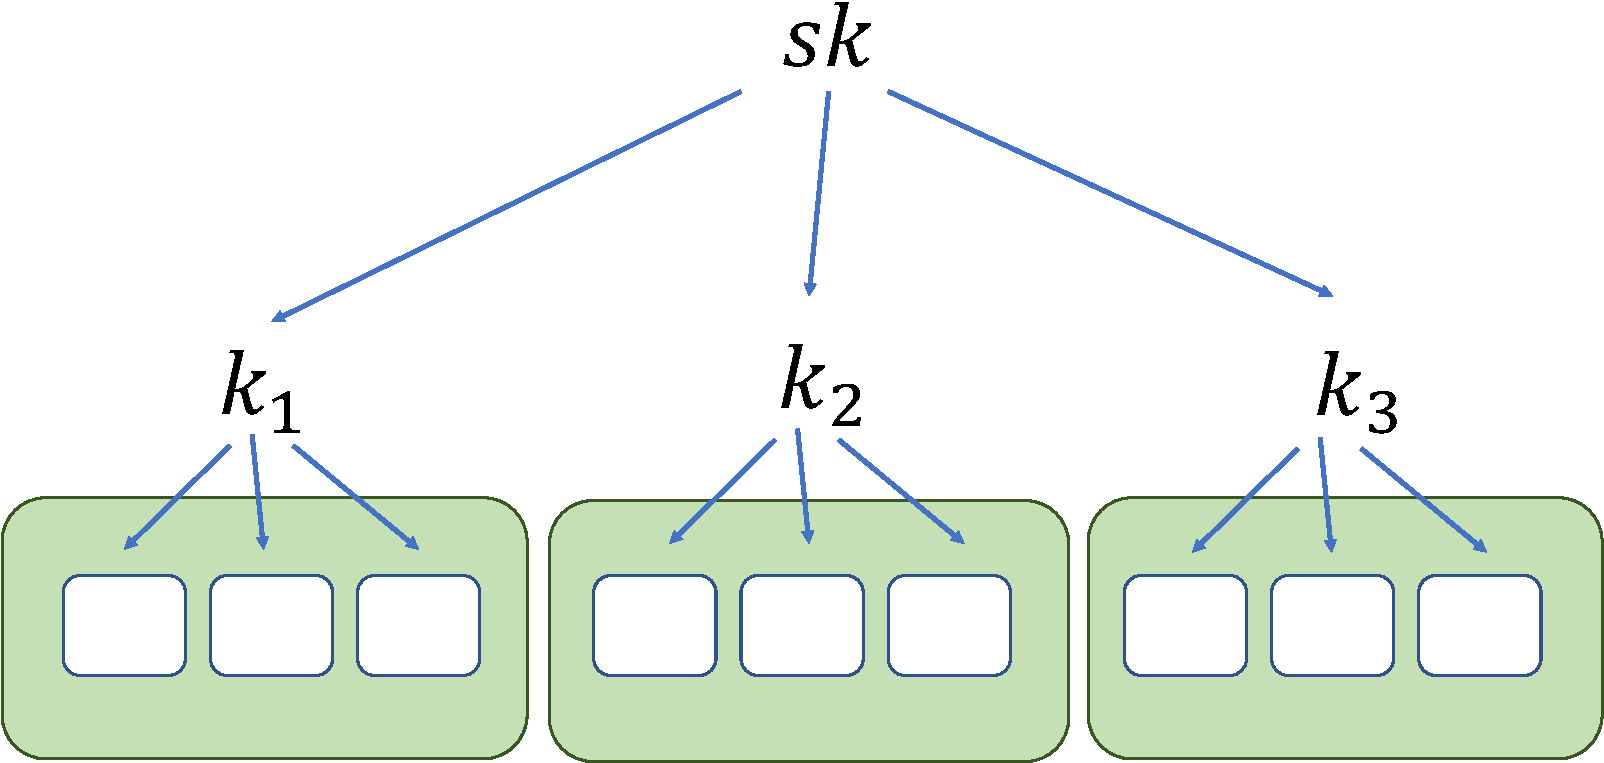
\includegraphics[width=0.6\linewidth]{figs/set-rep.pdf}
%     \caption{Two-layer set representation\label{fig:set-rep}. The first layer key expands to $n^{1/4}$ sub-keys. Each sub-key controls a superblock and expands to $n^{1/4}$ offsets. Each offset in a chunk represents an index.}
% \end{figure*}

%Here, $x[i:j]$ means the bit string from the $i$-th bit to the $(j-1)$-th bit of $x$'s binary representation.

Now, the new $\Program$ procedure will work as follows: it will expand the key $\sk$ into its $n^{1/4}$ sub-keys $k_0,\dots,k_{n^{1/4}-1}$. It will expand the $\superblock(x)$-th
sub-key into $n^{1/4}$ offsets $\delta_0,\dots,\delta_{n^{1/4}-1}$. Let $y$ be a random element in $x$'s chunk and $k'$ be a uniformly random sub-key $k'\getr\{0,1\}^\lambda$. $\Program$ outputs the programmed key to be all the sub-keys $k_0,\dots,k_{n^{1/4}-1}$, except replacing $\superblock(x)$-th key with $k'$ and all the offsets 
replaces $x$'s offset to $y$'s offset and sends those $n^{1/4}$ offsets $\delta_0,\dots,\delta_{n^{1/4}-1}$, except replacing the offset corresponding to $x$ with $y$'s offset. Additionally, $\Program$ returns $\superblock(x)$ as the index $j$.

With this new definition of $\Program$, we also need to modify the definition of $\ListDecode$. On input the sub-keys $k_0',k_1',\ldots,k_{n^{1/4}-1}'$, and offsets $\delta_0',\delta_1',\ldots,\delta_{n^{1/4}-1}'$, 
$\ListDecode$ expands all the sub-keys to get $n^{1/4}$ offsets for each of them. For $i\in \{0,1,\ldots,n^{1/4}-1\}$, the server computes $S_i$ by considering the offsets for all superblocks other than the $i$-th superblock to be the offsets for their corresponding sub-keys and the offsets $\delta_0',\delta_1',\ldots,\delta_{n^{1/4}-1}'$ as the offsets of the $i$-th superblock.


We can now simply plug this new $\PPWPS$ construction into the existing structure of the single query protocol of $\Piano$ and get a protocol with $O(n^{1/4})$ online communication. In Section~\labelcref{sec:ppps} we formally define $\PPPS$ and describe and prove the security of our construction. 

\subsection{Supporting multiple queries in the online phase} 

Thus far, we have
given a new, low-communication protocol that handles only one query. We now want
to make $Q=\sqrt{n}/2$ queries with just one offline phase. For convenience, we
first make some assumptions about the queries without loss of generality, which
are also made in $\Piano$:
\begin{itemize}
    \item \textit{The client does not make repeated queries.} This can be ensured 
    by requiring the client to store a local cache of size $Q$ for caching the
    most recent $Q$ queries. If the client wants a repeated query, it can lookup
    in the cache and make a dummy query.
    
    \item \textit{The queries the client makes are on random indices.} This is a relatively
    strong assumption. However, we argue that it can be made without loss of
    generality and can be done by letting the client and the server agree on a
    pseudorandom permutation (PRP)~\cite{prp1,prp2} upfront and the server can
    permute the database according to the PRP. Another option is let the server
    build the database as a key-value storage and use a cuckoo hash
    table~\cite{cuckoo1,cuckoo2} directly based on a PRF to locate the queries.
    Notice that, in both implementations, the client can still make queries
    adaptively depending on the real query sequnce and the responses, which is
    sufficient for practical usage. Then, as long as the client makes the
    queries independent of the randomness of the PRP/PRF, those queries can be
    considered as uniformly random. This assumption is only needed for the
    correctness.
\end{itemize}

% What was d

% In order to support multiple queries, the key idea that had been used in
% $\Piano$ was to ``refresh" the consumed hint by re-programming a fresh hint in a
% way that does not change the distribution of the hints. Here, while our high
% level goal will be the same, our strategy to do it would be significantly
% different. The reason why the approach used in $\Piano$ does not translate here
% is because of the following tension. Since in this new protocol we compress
% bandwidth by making the client send only \emph{sub-keys} for the superblocks,
% re-programming the hint while still having this compression would make
% distribution of the client's future messages depend on the current query, which
% violates privacy. Therefore, we seem to require newer ideas to avoid this issue.

We will first show how to handle multiple queries when we have two-servers. We will use the additional server \emph{only} for ``refreshing'' the $\PPWPS$ after they have been consumed during an online query. The key idea is suppose $x$ was the queried index and the query returned answer $p_x$, we will sample a new secret $\PPWPS$ key $\sk'$ subject to $x\in\Set(\sk')$. We will program this key using $\Program$ at $\chunk(x)$.



\end{document}

